\documentclass[letterpaper,12pt,oneside,final]{book}
%\documentclass[letterpaper,12pt,oneside,draft]{book}
%%
%%  Gabarit de mémoire de maîtrise ou thèse de doctorat.
%%  Template for dissertations and theses @ Polytechnique Montreal.

%%  Normalement, il n'est pas nécessaire de modifier ce document
%%  sauf pour établir le langage (français ou anglais) et pour changer les noms des 
%%  fichiers à inclure.
%%  Usually, this document needs to be modified only to set up the language (French or English) 
%%  and to change the names of the files to include.
%%
%%  Version: 2018-07-31
%%
%%  Accepte les caractères accentués dans le document (UTF-8).


\makeatletter
\def\bstctlcite{\@ifnextchar[{\@bstctlcite}{\@bstctlcite[@auxout]}}
\def\@bstctlcite[#1]#2{\@bsphack
 \@for\@citeb:=#2\do{%
   \edef\@citeb{\expandafter\@firstofone\@citeb}%
   \if@filesw\immediate\write\csname #1\endcsname{\string\citation{\@citeb}}\fi}%
 \@esphack}
\makeatother

% LA COMMANDE SUIVANTE ÉTABLIT LE LANGAGE DE LA THÈSE : ÉCRIRE french POUR UNE THÈSE EN FRANÇAIS
% THE NEXT COMMAND DETERMINES THE LANGUAGE OF THE THESIS: WRITE english FOR A THESIS IN ENGLISH
\newcommand\Langue{french}            

\usepackage{ifthen}
\usepackage[utf8]{inputenc}
%%
%% Support pour l'anglais et le français (français par défaut).
%\usepackage[cyr]{aeguill}
\usepackage{lmodern}      % Police de caractères plus complète et généralement indistinguable visuellement de la police standard de LaTeX (Computer Modern).
\usepackage[T1]{fontenc}  % Bon encodage des caractères pour qu'Acrobat Reader reconnaisse les accents et les ligatures telles que ffi.

% le langage par défaut est le dernier de la liste, c'est-à-dire français
\ifthenelse{\equal{\Langue}{english}}{
	\usepackage[french,english]{babel}
}{
	\usepackage[english,french]{babel} 
}

%%
%% Charge le module d'affichage graphique.
\usepackage{graphicx}

\usepackage{epstopdf}  % Permet d'utiliser des .eps avec pdfLaTeX.
%%
%% Recherche des images dans les répertoires.
\graphicspath{{./images/}{./images_article1/}{./images_article2/}{./images_theme3/}}
%%
%% Un float peut apparaître seulement après sa définition, jamais avant.
\usepackage{flafter,placeins}
%%
%% Utilisation de natbib pour les citations et la bibliographie.
%\usepackage{natbib}
\usepackage[numbers,sort&compress]{natbib} % Permet de comprimer les citations lorsqu'elle sont séquentielles 
\usepackage{notoccite}
%%
%% Autres packages.
\usepackage{amsmath,color,soulutf8,longtable,colortbl,setspace,xspace,url,pdflscape}
%\usepackage{cite}
\usepackage[list-units = single, range-units = single]{siunitx}
\sisetup{separate-uncertainty}
\addto\extrasfrench{\sisetup{locale = FR}} % Change le séparateur de décimale pour une virgule dans les sectione en français de la thèse et laisse un point dans les sections anglaises


\usepackage{placeins} % For /Floatbarrier
\usepackage{array,booktabs}
\usepackage{float}
\usepackage{upgreek}
\usepackage{chemformula}
\usepackage{gensymb} % Pour \ohm
\usepackage{amssymb}

\usepackage{chemfig}

\usepackage{subfigure}

\usepackage{paralist}

\usepackage{tikz}
\usetikzlibrary{arrows,arrows.meta,shapes,positioning,shadows,trees}
\usetikzlibrary{decorations.pathmorphing}

%%
%% Support des acronymes.
\usepackage[nolist]{acronym}
\onehalfspacing                % Interligne 1.5.
%%
%% Définition d'un style de page avec seulement le numéro de page à
%% droite. On s'assure aussi que le style de page par défaut soit
%% d'afficher le numéro de page en haut à droite.
\usepackage{fancyhdr}
\fancypagestyle{pagenumber}{\fancyhf{}\fancyhead[R]{\thepage}}
\renewcommand\headrulewidth{0pt}
\makeatletter
\let\ps@plain=\ps@pagenumber
\makeatother
%%
%% Module qui permet la création des bookmarks dans un fichier PDF.
%\usepackage[dvipdfm]{hyperref}
\usepackage{hyperref}
\usepackage{caption}  % Hyperlien vers la figure plutôt que son titre.
\makeatletter
\providecommand*{\toclevel@compteur}{0}
\makeatother
%%
%% Définitions spécifiques au format de rédaction de Poly.
%% Here we define the Poly formatting.
\RequirePackage[\Langue]{MemoireThese}
%%
%% Définitions spécifiques à l'étudiant.
%% -----------------------------------
%% ---> À MODIFIER PAR L'ETUDIANT / TO BE MODIFIED BY THE STUDENT <---
%% -----------------------------------
%%
%% Commandes qui affichent le titre du document, le nom de l'auteur, etc.
\newcommand\monTitre{Développement d'un nanocomposite conducteur pour le soudage par résistance des composites thermoplastiques}
\newcommand\monPrenom{David}
\newcommand\monNom{Brassard}
\newcommand\monDepartement{génie chimique}  % Department
\newcommand\maDiscipline{Génie chimique}
\newcommand\monDiplome{D}        % (M)aîtrise ou (D)octorat / (M)aster or Ph(D)
\newcommand\anneeDepot{2020}    % Year
\newcommand\moisDepot{Février}       % Month
\newcommand\monSexe{M}           % "M" ou "F" = Gender
\newcommand\PageGarde{N}         % "O" ou "N" = Yes or No
\newcommand\AnnexesPresentes{O}  % "O" ou "N". Indique si le document comprend des annexes. / If the thesis includes annexes = O or N = No.
\newcommand\mesMotsClef{Composites thermoplastiques, Soudage, Soudage par Résistance, Nanocomposite}
%%  DEFINITION DU / OF JURY
%%
%%  Pour la définition du jury, les macros suivantes sont definies:
%%  \PresidentJury, \DirecteurRecherche, \CoDirecteurRecherche, \MembreJury, \MembreExterneJury
%%
%%  Toutes les macros prennent 3 paramètres: Sexe (M/F), Nom, Prénom
%%  All the macros have 3 parameters: Sex (M/F), Last name, First name
\newcommand\monJury{\PresidentJury{F}{Heuzey}{Marie-Claude}\\
\DirecteurRecherche{M}{R. Tavares}{Jason}\\
\CoDirecteurRecherche{F}{Dubé}{Martine}\\
\MembreJury{M}{Favis}{Basil}\\
\MembreExterneJury{M}{Rodrigue}{Denis}}


\ifthenelse{\equal{\monDiplome}{M}}{
\newcommand\monSujet{Mémoire de maîtrise}
\newcommand\monDipl{Maîtrise ès sciences appliquées}
}{
\newcommand\monSujet{Thèse de doctorat}
\newcommand\monDipl{Philosophi\ae{} Doctor}
}
%%
%% Informations qui sont stockées dans un fichier PDF.
\hypersetup{
  pdftitle={\monTitre},
  pdfsubject={\monSujet},
  pdfauthor={\monPrenom{} \monNom},
  pdfkeywords={\mesMotsClef},
  bookmarksnumbered,
  pdfstartview={FitV},
  hidelinks,
  linktoc=all
}
%%
%% Il y a un document par chapitre du mémoire.
%%

\newcolumntype{L}[1]{>{\raggedright\let\newline\\\arraybackslash\hspace{0pt}}m{#1}}
\newcolumntype{C}[1]{>{\centering\let\newline\\\arraybackslash\hspace{0pt}}m{#1}}

\begin{document}
%\bstctlcite{IEEEexample:BSTcontrol}

%%
%% Page de titre du mémoire.
\frontmatter
% Compte optionellement la page de garde dans la pagination.
\ifthenelse{\equal{\PageGarde}{O}}{\addtocounter{page}{1}}{}
\thispagestyle{empty}%
\begin{center}%
\vspace*{\stretch{0.1}}
\textbf{POLYTECHNIQUE MONTRÉAL}\\
affiliée à l'Université de Montréal\\
\vspace*{\stretch{1}}
\textbf{\monTitre}\\
\vspace*{\stretch{1}}
\textbf{\MakeUppercase{\monPrenom~\monNom}}\\
Département de~{\monDepartement}\\
\vspace*{\stretch{1}}
\ifthenelse{\equal{\monDiplome}{M}}{Mémoire présenté}{Thèse présentée} en vue de l'obtention du diplôme de~\emph{\monDipl}\\
\maDiscipline\\
\vskip 0.4in
\moisDepot~\anneeDepot
\end{center}%
\vspace*{\stretch{1}}
\copyright~\monPrenom~\monNom, \anneeDepot.
%%
%% Identification des membres du jury.
%%
\newpage\thispagestyle{empty}%
\begin{center}%

\vspace*{\stretch{0.1}}
\textbf{POLYTECHNIQUE MONTRÉAL}\\
affiliée à l'Université de Montréal\\
\vspace*{\stretch{2}}
Ce\ifthenelse{\equal{\monDiplome}{M}}{~mémoire intitulé}{tte thèse intitulée} :\\
\vspace*{\stretch{1}}
\textbf{\monTitre}\\
\vspace*{\stretch{1}}
présenté\ifthenelse{\equal{\monDiplome}{M}}{}{e}
par~\textbf{\mbox{\monPrenom~\MakeUppercase{\monNom}}}\\
en vue de l'obtention du diplôme de~\emph{\mbox{\monDipl}}\\
a été dûment accepté\ifthenelse{\equal{\monDiplome}{M}}{}{e} par le jury d'examen constitué de :\end{center}
\vspace*{\stretch{2}}
\monJury
%%
\pagestyle{pagenumber}%
%% Dédicace
%%
%% La dédicace est un hommage que l'auteur souhaite
%% rendre à une ou plusieurs personnes de son choix.
%%
\ifthenelse{\equal{\Langue}{english}}{
	\chapter*{DEDICATION}\thispagestyle{headings}
	\addcontentsline{toc}{compteur}{DEDICATION}
}{
	\chapter*{DÉDICACE}\thispagestyle{headings}
	\addcontentsline{toc}{compteur}{DÉDICACE}
}

\begin{flushright}
  \itshape
  Pour toutes ces questions \\
  en quête de réponses
\end{flushright}
          % Dédicace du document.
\selectlanguage{french}
% Remerciements / Acknowledgements
%
%  Grâce aux remerciements, l'auteur attire l'attention du lecteur
% sur l'aide que certaines personnes lui ont apportée, sur leurs
% conseils ou sur toute autre forme de contribution lors de la
% réalisation de son mémoire. Le cas échéant, c'est dans cette section
% que le candidat doit témoigner sa reconnaissance à son directeur de
% recherche, aux organismes dispensateurs de subventions ou aux
% entreprises qui lui ont accordé des bourses ou des fonds de
% recherche.
\ifthenelse{\equal{\Langue}{english}}{
	\chapter*{ACKNOWLEDGEMENTS}\thispagestyle{headings}
	\addcontentsline{toc}{compteur}{ACKNOWLEDGEMENTS}
}{
	\chapter*{REMERCIEMENTS}\thispagestyle{headings}
	\addcontentsline{toc}{compteur}{REMERCIEMENTS}
}
%
Je tiens tout d'abord à remercier spécialement ma femme Marie-Pier pour son support, sa compréhension et son amour sans faille. 
Je veux aussi remercier Edmond et Simone de s'être occupés de me changer les idées lorsque j'étais en dehors de l'école et pour leur compréhension quand leur papa devait vraiment travailler. 

Pour avoir cru en moi et pour m'avoir offert tous les conseils et le support qu'ils pouvaient m'offrir, je voudrais remercier Jason R. Tavares et Martine Dubé. 
Pour ses conseils quand est venu le temps de parler de mélanges de polymères et de diffusion, merci à Nick Virgilio. 
Merci à Marie-Claude Heuzey pour notre collaboration pour le cours Matériaux polymères. 
Merci à Bruno Blais et à David Vidal pour les discussions du midi et pour leurs réponses à mes questions de modélisation. 

Merci à tous mes collègues de laboratoire à Polytechnique: Wendell pour son éternelle bonne humeur, Hamed pour les parties d'échecs, Faezeh qui sait voir le meilleur côté des gens, Simon pour avoir amené plus de Linux au bureau, Alessio pour sa curiosité, Charles et Mélanie pour les compétitions de pâtisseries, Martin, Christina, Sergio, Alice, Somayeh, Ulrich.

Merci aussi à mes collègues hors Polytechnique: Vincent Rohart, Laurent Cormier, Louis-Charles Forcier, Nicolas Côté, Corentin Bobet, Félix Lessard, Adrien Métafiot. 

Merci à tous le personnel de support du département de génie chimique: Daniel et Matthieu pour leurs innombrables services, Martine et Gino pour leur bonne humeur contagieuse, Claire, Richard, Sébastien, Anic, Robert, Alexandre, Carmen, Brigitte. 

Merci aussi à Serge Plamondon et Nabil Mazeghrane de l'ÉTS. 

Je veux remercier Brigitte Defoort, Guy Larnac et Philippe Briant d'ArianeGroup pour avoir cru en ce projet ainsi que pour le temps et le financement qu'ils y ont consacrés. 

Je tiens finalement à remercier Mme Danièle Dumais et la Fondation Polytechnique pour la bourse Neil R. Mitchell \& Danièle Dumais. 
     % Remerciements.
\selectlanguage{french}
% Résumé du mémoire.
%
\chapter*{RÉSUMÉ}\thispagestyle{headings}
\addcontentsline{toc}{compteur}{RÉSUMÉ}

Le soudage par résistance est une méthode rapide et efficace pour joindre des pièces en composites thermoplastiques. 
En collaboration avec le partenaire industriel, ArianeGroup, ce projet a pour but de développer un élément chauffant nanocomposite pouvant servir à produire une jonction flexible en soudant des pièces de composite thermoplastique et d'élastomère thermoplastique.
Le développement de ce joint flexible soudé a pour but de remplacer une jonction par adhésifs entre les réservoirs et les jupettes sur un lanceur de satellite. 
Le développement de ce joint a été réalisé en 4 étapes. 
Tout d'abord, il a été nécessaire de concevoir un nanocomposite conducteur aux propriétés adaptées pour servir d'élément chauffant durant le soudage par résistance. 
Par la suite, cet élément chauffant a été utilisé pour développer un procédé de soudage entre des adhérents en composite thermoplastique. 
Ensuite, une fenêtre d'opération a été établie afin d'améliorer notre contrôle du procédé ainsi que les performances des joints obtenus. 
Finalement, l'élément chauffant nanocomposite a été employé afin de développer un procédé de soudage avec un élastomère thermoplastique afin de former une jonction flexible. 

Afin d'obtenir les propriétés électriques requises pour le soudage et après avoir évalué plusieurs compositions, un nanocomposite composé d'une matrice de polyétherimide (PEI) et d'une fraction massique de 10\% de nanotubes de carbone a été sélectionné. 
En raison d'un manque de reproductibilité dans les résultats lorsque le contrôle du procédé était effectué en employant un voltage constant, un mode de contrôle à puissance constante a été développé et appliqué avec succès pour produire des jonctions soudées avec l'élément chauffant nanocomposite.  

En utilisant les données recueillies durant les essais de soudage, un modèle par éléments finis a été développé afin de prévoir la distribution de température dans le joint et d'établir la fenêtre d'opération. 
Avec celle-ci, des essais complémentaires de soudage ont été réalisés et une résistance maximale de \SI[locale=FR]{24.9}{\mega\pascal} a été atteinte lors d'essais en simple cisaillement, soit une amélioration de 28\% par rapport aux résultats précédents. 
Les températures atteintes dans le joint lors des essais de soudage sont cependant plus élevées que les températures traditionnellement nécessaires avec un élément chauffant en acier inoxydable et entrainent de la dégradation thermique dans le joint. 
Il est postulé que la forte fraction de nanotubes de carbone limite la mobilité des chaines de polymère et retarde ainsi le soudage. 
De plus, la forte proportion de nanotubes réduit grandement la ductilité ainsi que la résistance du nanocomposite. 

Les derniers travaux présentés se sont ensuite concentrés sur le développement d'un procédé de soudage pour produire une jonction flexible avec un élastomère thermoplastique. 
Après des essais infructueux avec des élastomères SIS et SEBS, des résultats encourageants ont été obtenus lors d'essais de soudage isotherme avec l'élastomère PEI-siloxane dans une étuve sous vide et avec une presse chauffante. 
Malgré sa bonne stabilité thermique à température élevée, cet élastomère n'a pas réussi à produire une soudure rencontrant les cibles de performance d'ArianeGroup. 
Encore une fois, la température élevée du procédé et le manque de mobilité des chaines pourraient être les causes de ces résultats négatifs. 

Finalement, en se basant sur les résultats obtenus, des pistes de recherche sont proposées afin d'améliorer le procédé de soudage par résistance avec un élément chauffant nanocomposite. 





%Le résumé est un bref exposé du sujet traité, des objectifs visés,
%des hypothèses émises, des méthodes expérimentales utilisées et de
%l'analyse des résultats obtenus. On y présente également les
%principales conclusions de la recherche ainsi que ses applications
%éventuelles. En général, un résumé ne dépasse pas quatre pages.
%
%Le résumé doit donner une idée exacte du contenu du mémoire ou de la thèse. Ce ne
%peut pas être une simple énumération des parties du document, car il
%doit faire ressortir l'originalité de la recherche, son aspect
%créatif et sa contribution au développement de la technologie ou à
%l'avancement des connaissances en génie et en sciences appliquées.
%Un résumé ne doit jamais comporter de références ou de figures.
      % Résumé du sujet en français.
% Abstract
%
% Résumé de la recherche écrit en anglais sans être
% une traduction mot à mot du résumé écrit en français.

\chapter*{ABSTRACT}\thispagestyle{headings}
\addcontentsline{toc}{compteur}{ABSTRACT}
%
\begin{otherlanguage}{english}
	
	Resistance welding is a quick and efficient way to join thermoplastic composite parts. 
	In collaboration with the industrial partner, ArianeGroup, this project develops a nanocomposite heating element to produce a flexible junction by welding thermoplastic composite parts to a thermoplastic elastomer. 
	This welded flexible joint will replace an adhesive bonded junction between the tanks and skirts of a satellite launcher. 
	Development of this joint was done in 4 stages. 
	First, it was necessary to develop a conductive nanocomposite with appropriate properties to serve as a heating element during resistance welding. 
	This heating element then served to develop a resistance welding process between thermoplastic composite adherents. 
	Following that, a process window was established to improve our control over the process and the performance of the joints. 
	Finally, the nanocomposite heating element served to develop a resistance welding process with a thermoplastic elastomer to form a flexible joint. 
	
	To obtain the electrical properties required to serve as a heating element and after having evaluated many compositions, a nanocomposite composed of PEI and 10\% weight fraction of MWCNT was selected. 
	Due to the variability in the results obtained under constant voltage operation of the power source, a constant power control mode was developed and successfully applied to produce welded joints with the nanocomposite heating element. 
	
	By using the data acquired during welding experiments, a finite element model was developed to predict the temperature profile in the weld and to establish a window of operation. 
	With this widow of operation, supplementary welding tests were performed and a lap shear strength of \SI{24.9}{\mega\pascal} was reached, an improvement of 28\% over our previous results. 
	The temperatures reached within the joint during welding experiments are, however, higher than temperatures traditionally necessary to obtain a weld with a stainless steel heating element, leading to thermal degradation. 
	It is assumed that the high mass fraction of MWCNT limits the polymer chain's mobility and delays their diffusion. 
	Furthermore, the high mass fraction of MWCNT reduces the ductility and strength of the nanocomposite. 
	
	The last portion of this work focusses on the development of a resistance welding process to produce flexible joints with a thermoplastic elastomer. 
	After unsuccessful attempts with SIS and SEBS elastomers, encouraging results were obtained during isothermal welding tests in a vacuum oven and a hot press with a PEI-siloxane elastomer. 
	Despite its good thermal stability at high temperature, welding tests with this elastomer did not produce joints meeting the performance targets of ArianeGroup. 
	Once again, the elevated temperature during the process combined with the reduced mobility of the polymer chains could be the causes of these negative results. 
	
	Finally, based on the results obtained, research topics to improve the resistance welding process with a nanocomposite heating element are proposed. 
	
\end{otherlanguage}
          % Résumé du sujet en anglais.

{\setlength{\parskip}{0pt}
%%
%% Table des matières.
\ifthenelse{\equal{\Langue}{english}}{
	\renewcommand\contentsname{TABLE OF CONTENTS}
}{
	\renewcommand\contentsname{TABLE DES MATIÈRES}
}
\tableofcontents
%%
%% Liste des tableaux.
\ifthenelse{\equal{\Langue}{english}}{
	\renewcommand\listtablename{LIST OF TABLES}
}{
	\renewcommand\listtablename{LISTE DES TABLEAUX}
}\listoftables
%%
%% Table des figures.
\ifthenelse{\equal{\Langue}{english}}{
	\renewcommand\listfigurename{LIST OF FIGURES}
}{
	\renewcommand\listfigurename{LISTE DES FIGURES}
}\listoffigures
%%
%% Liste des annexes au besoin.
}

\chapter*{LISTE DES ABRÉVIATIONS}
\addcontentsline{toc}{compteur}{LISTE DES ABRÉVIATIONS}
\pagestyle{pagenumber}
%
\begin{acronym}
	\acro{AFP}{Automated fibre placement}
	\acro{CF}{Fibres de carbone}
	\acro{FEM}{Modèle par éléments finis}
	\acro{FTIR}{Spectroscopie infrarouge à transformée de Fourier}
	\acro{HE}{Élément chauffant}
	\acro{LSS}{Résistance en cisaillement}
	\acro{MWCNT}{Nanotubes de carbone multiparois}
	\acro{PEEK}{Polyétheréthercétone}
	\acro{PEI}{Polyétherimide}
	\acro{REV}{Volume élémentaire représentatif}français
	\acro{TPC}{Composite à matrice thermoplastique}
	\acro{SLS}{Simple cisaillement}
	\acro{SS}{Acier inoxydable}
	\acro{UD}{Unidirectionnel}
\end{acronym}
%
\begin{longtable}{p{0.75in}>{\raggedright\arraybackslash}p{2.5in} p{2.5in}}
	      & \textbf{Français}                                              & \textbf{Anglais}                                                \\
	AFP   & Déposition automatisée de fibres                               & Automated fibre placement                                       \\
	CF    & Fibres de carbone                                              & Carbon Fibre                                                    \\
	FEM   & Modèle par éléments finis                                      & Finite element model                                            \\
	FTIR  & Spectroscopie infrarouge à transformée de Fourier              & Fourier-transform infrared spectroscopy                         \\
	HE    & Élément chauffant                                              & Heating element                                                 \\
	LSS   & Résistance en cisaillement                                     & Lap shear strength                                              \\
	MWCNT & Nanotubes de carbone multiparois                               & Multi-Walled Carbon Nanotubes                                   \\
	PEEK  & Polyétheréthercétone                                           & poly(ether ether ketone)                                        \\
	PEI   & Polyétherimides                                                & Polyetherimide                                                  \\
	TPC   & Composite à matrice thermoplastique                            & Thermoplastic composite                                         \\
	REV   & Volume élémentaire représentatif                               & Representative elementary volumes                               \\
	SEBS  & Copolymère polystyrène-b-poly(éthylène-butylène)-b-polystyrène & Polystyrene-block-polyisoprene-block-polystyrene                \\
	SIS   & Copolymère polystyrène-b-polyisoprène-b-polystyrène            & Polystyrene-block-poly(ethylene-ran-butylene)-block-polystyrene \\
	SLS   & Simple cisaillement                                            & Single lap shear                                                \\
	SS    & Acier inoxydable                                               & Stainless steel                                                 \\
	TGA   & Analyse thermogravimétrique                                    & Thermogravimetric analysis                                      \\
	UD    & Unidirectionnel                                                & Unidirectional
\end{longtable}
       % Liste des sigles et abréviations.
\chapter*{LISTE DES SYMBOLES}
\addcontentsline{toc}{compteur}{LISTE DES SYMBOLES}
\pagestyle{pagenumber}
%

%
\begin{longtable}{l p{2.5cm} p{4in}}
	\textbf{Symboles} & \textbf{Unité}                                      & \textbf{Définition}                                                                   \\
	\endhead
	$A_s$             & [\si{\square\metre}]                                & Aire de la section du conducteur                                                      \\
	$a^*$             & [ \ ]                                               & Paramètre géométrique                                                                 \\
	$E$               & [\si{\joule}]                                       & Énergie                                                                               \\
	$\mathbf{E}$      & [\si{\volt\per\metre}]                              & Densité du champ électrique                                                           \\
	$\mathbf{J_e}$    & [\si{\ampere\per\square\metre}]                     & Densité du courant d'électrons                                                        \\
	$\mathbf{J}$      & [\si{\ampere\per\square\metre}]                     & Densité de courant                                                                    \\
	$\mathbf{n_1}$    & [ \ ]                                               & Vecteur normal pointant vers l'extérieur du matériau 1                                \\
	$\mathbf{n_2}$    & [ \ ]                                               & Vecteur normal pointant vers l'extérieur du matériau 2                                \\
	$\mathbf{n}$      & [ \ ]                                               & Vecteur normal                                                                        \\
	$\mathbf{q}$      & [\si{\watt\per\square\metre}]                       & Flux de chaleur                                                                       \\
	$\nabla T$        & [\si{\kelvin\per\metre}]                            & Gradient de température                                                               \\
	$\nabla T_1$      & [\si{\kelvin\per\metre}]                            & Gradient de température dans le matériau 1                                            \\
	$\nabla T_2$      & [\si{\kelvin\per\metre}]                            & Gradient de température dans le matériau 2                                            \\
	$C_p$             & [\si{\joule\per\kilogram\per\kelvin}]               & Chaleur massique à pression constante                                                 \\
	$D_{ic}$          & [ \ ]                                               & Degré de contact intime                                                               \\
	$d$               & [\si{\metre}]                                       & Diamètre                                                                              \\
	$g$               & [\si{\metre\per\square\second}]                     & Accélération due à la gravité terrestre                                               \\
	$\Delta G_m$      & [\si{\joule}]                                       & Énergie libre de Gibbs                                                                \\
	$Gr_L$            & [ \ ]                                               & Nombre de Grashof pour une plaque verticale                                           \\
	$h_{conv}$        & [\si{\watt\per\square\metre\per\kelvin}]            & Coefficient de convection                                                             \\
	$h$               & [\si{\watt\per\square\metre\per\kelvin}]            & Conductance de contact thermique totale                                               \\
	$H_c$             & [\si{\pascal}]                                      & Microdureté                                                                           \\
	$h_c$             & [\si{\watt\per\square\metre\per\kelvin}]            & Conductance de contact                                                                \\
	$h_g$             & [\si{\watt\per\square\metre\per\kelvin}]            & Conductance du gaz interstitiel                                                       \\
	$I$               & [\si{\ampere}]                                      & Intensité du courant                                                                  \\
	$k$               & [\si{\watt\per\metre\per\kelvin}]                   & Conductivité thermique                                                                \\
	$k_1$             & [\si{\watt\per\metre\per\kelvin}]                   & Conductivité thermique du matériau 1                                                  \\
	$k_2$             & [\si{\watt\per\metre\per\kelvin}]                   & Conductivité thermique du matériau 2                                                  \\
	$k_{contact}$     & [\si{\watt\per\metre\per\kelvin}]                   & Moyenne harmonique des conductivités des surfaces en contact                          \\
	$L$               & [\si{\metre}]                                       & Hauteur                                                                               \\
	$L$               & [\si{\metre}]                                       & Moitié de la distance moyenne entre les particules                                    \\
	$L_c$             & [\si{\metre}]                                       & Longueur caractéristique                                                              \\
	$l$               & [\si{\metre}]                                       & Longueur du conducteur                                                                \\
	$l(t)$            & [\si{\metre}]                                       & Longueur moyenne des chaînes mineures ayant traversé l'interface en fonction du temps \\
	$M$               & [\si{\kilogram\per\mole}]                           & Masse moléculaire                                                                     \\
	$m_{asp,1}$       & [ \ ]                                               & Pente moyenne des aspérités (rugosité) du matériau 1                                  \\
	$m_{asp,2}$       & [ \ ]                                               & Pente moyenne des aspérités (rugosité) du matériau 2                                  \\
	$m_{asp}$         & [ \ ]                                               & Pente moyenne des aspérités (rugosité) du matériau                                    \\
	$Nu$              & [ \ ]                                               & Nombre de Nusselt                                                                     \\
	$n_1$             & [ \ ]                                               & Nombre de moles du composant 1                                                        \\
	$n_2$             & [ \ ]                                               & Nombre de moles du composant 2                                                        \\
	$P$               & [\si{\watt}]                                        & Puissance                                                                             \\
	$P_{app}$         & [\si{\pascal}]                                      & Pression appliquée                                                                    \\
	$Pr$              & [ \ ]                                               & Nombre de Prandtl                                                                     \\
	$p$               & [\si{\mega\pascal}]                                 & Pression de contact                                                                   \\
	$Q_e$             & [W\,m$^{-3}$]                                       & Source de chaleur électromagnétique                                                   \\
	$Q_j$             & [\si{\ampere\per\square\metre}]                     & Source de courant                                                                     \\
	$R_m$             & [\si{\joule\per\mole\per\kelvin}]                   & Constante universelle des gaz parfaits                                                \\
	$R_e$             & [\si{\ohm}]                                         & Résistance                                                                            \\
	$T$               & [\si{\kelvin} ]                                     & Température                                                                           \\
	$T_s$             & [\si{\kelvin} ]                                     & Température de surface                                                                \\
	$T_{\infty}$      & [\si{\kelvin} ]                                     & Température ambiante                                                                  \\
	$t$               & [\si{\second} ]                                     & Temps                                                                                 \\
	$t_c$             & [\si{\second} ]                                     & Temps de contact                                                                      \\
	$t_D$             & [\si{\second}]                                      & Constante de temps pour la diffusion thermique                                        \\
	$t_r$             & [\si{\second}]                                      & Temps de reptation                                                                    \\
	$V$               & [\si{\volt} ]                                       & Potentiel électrique                                                                  \\
	$v_f$             & [ \ ]                                               & Fraction volumique de fibres                                                          \\
	$w^*$             & [ \ ]                                               & Paramètre géométrique                                                                 \\
	$\alpha$          & [\si{\square\metre\per\second}]                     & Diffusivité thermique                                                                 \\
	$\beta$           & [\si{\per\celsius}]                                 & Coefficient d'expansion thermique de l'air                                            \\
	$\varepsilon$     & [ \ ]                                               & Émissivité de surface                                                                 \\
	$\varepsilon_0$   & [\si{\farad\per\metre}]                             & Permittivité du vide                                                                  \\
	$\varepsilon_r$   & [ \ ]                                               & Permittivité relative                                                                 \\
	$\lambda_{air}$   & [\si{\watt\per\square\metre\per\kelvin}]            & Conductivité thermique de l'air                                                       \\
	$\mu$             & [\si{\pascal\second}]                               & Viscosité dynamique                                                                   \\
	$\mu_{mf}$        & [\si{\pascal\second}]                               & Vicosité                                                                              \\
	$\nu$             & [\si{\square\metre\per\second}]                     & Viscosité cinématique                                                                 \\
	$\rho$            & [\si{\kilogram\per\cubic\metre}]                    & Densité                                                                               \\
	$\rho_{ele}$      & [\si{\ohm\metre}]                                   & Résistivité                                                                           \\
	$\sigma$          & [\si{\siemens\per\metre}]                           & Conductivité électrique                                                               \\
	$\sigma_{asp,1}$  & [\si{\metre}]                                       & Hauteur moyenne des aspérités (rugosité) du matériau 1                                \\
	$\sigma_{asp,2}$  & [\si{\metre}]                                       & Hauteur moyenne des aspérités (rugosité) du matériau 2                                \\
	$\sigma_{asp}$    & [\si{\metre}]                                       & Hauteur moyenne des aspérités (rugosité)                                              \\
	$\sigma_{SB}$     & [\si{\watt\per\square\metre\per\raiseto{4}\kelvin}] & Constante de Stefan–Boltzmann                                                         \\
	$\phi_1$          & [ \ ]                                               & Fraction volumique du composant 1                                                     \\
	$\phi_2$          & [ \ ]                                               & Fraction volumique du composant 2                                                     \\
	$\chi_{12}$       & [ \ ]                                               & Paramètre $\chi$ entre les composants 1 et 2                                          \\
	$\chi(t)$         & [\si{\metre}]                                       & Distance moyenne d'interpénétration des monomères en fonction du temps
\end{longtable}
       % Liste des sigles et abréviations.
\ifthenelse{\equal{\AnnexesPresentes}{O}}{\listofappendices}{}
\mainmatter
% Dans l'introduction, on présente le problème étudié et les buts
% poursuivis. L'introduction permet de faire connaître le cadre de la
% recherche et d'en préciser le domaine d'application. Elle fournit
% les précisions nécessaires en ce qui concerne le contexte de
% réalisation de la recherche, l'approche envisagée, l'évolution de
% la réalisation. En fait, l'introduction présente au lecteur ce
% qu'il doit savoir pour comprendre la recherche et en connaître la
% portée.
\selectlanguage{french}
\Chapter{INTRODUCTION}\label{sec:Introduction}  % 10-12 lignes pour introduire le sujet.

Même si on ne les voit pas, les satellites artificiels sont essentiels à la société moderne. 
Ils permettent d'acquérir des données scientifiques importantes dans des domaines tels que l'astronomie \cite{Freedman2001}, l'étude des plaques tectoniques et des volcans \cite{Christodoulidis1985}, la climatologie \cite{Hollmann2013}, le suivi de l'état des glaciers \cite{Goldstein1993} ou l'analyse de l'état de l'atmosphère \cite{Laube2014}. 
Également, ils ont de nombreuses applications civiles telles que les prévisions météorologiques \cite{Bauer2015}, la navigation \cite{Getting1993}, les télécommunications \cite{Evans2005}, l'agriculture \cite{Lobell2002} ou la mesure de l'étendue des désastres majeurs \cite{Tralli2005}.  
Qu'ils soient opérés par des entités gouvernementales ou privées, tous les satellites doivent être positionnés en orbite à l'aide de lanceurs de satellites. 
Ces derniers doivent garantir des niveaux de fiabilité très élevés et livrer avec une très grande précision les satellites sur les trajectoires convenues tout en minimisant les couts. 

Le potentiel commercial d'un lanceur de satellite est fortement lié au ratio entre la masse utile qu'il peut élever en orbite et sa masse. 
Afin d'optimiser ce ratio, il est nécessaire de sélectionner des matériaux offrant de bonnes propriétés mécaniques ainsi qu'un poids minimal. 
Les matériaux composites permettent d'atteindre ces deux buts en permettant de créer des pièces aux propriétés optimisées en fonction de l'application, et ce, tout en minimisant leur masse. 
Le développement d'une nouvelle génération de lanceurs en matériaux composites est justifié par des impératifs techniques ainsi qu'économiques. 
Cependant, la transition vers les matériaux composites pose de nombreux défis. 

Dans la conception des lanceurs modernes, les réservoirs de carburant et de comburant agissent comme composants structurels et supportent le poids du lanceur et de la charge utile. 
Dans le cas \mbox{d'Ariane 6}, ces réservoirs ainsi que de nombreux composants en matériaux composites seront produits par déposition automatisée de fibres (AFP) ou par enroulement filamentaire avec une consolidation \textit{in situ} au laser \cite{Krzeminski2014}. 
Les jupettes quant à elles agissent comme éléments de transition entre les sections et les étages du lanceur. 
Ainsi, le joint structurel entre une jupette et un réservoir (Fig.~\ref{fig:schema_jonction}) doit supporter les forces rencontrées durant le décollage et est nécessaire au maintien de l'intégrité du lanceur. 
De plus, cette jonction doit être flexible, car, pendant le décollage, le diamètre des réservoirs change en fonction de leur pression interne résiduelle. 
Ces déformations doivent alors être absorbées par les joints avec les jupettes. 
L'emploi de jonctions flexibles permet également d'absorber une partie des vibrations causées lors du décollage et ainsi de minimiser les charges que doit supporter le chargement. 
Dans le cas d'assemblages de pièces en composite, une grande attention doit être portée aux jonctions entre les composants. 
Ces dernières sont généralement des points critiques pour la conception des structures. 
Dans ce cas particulier, la jonction entre la jupette et le réservoir présente des conditions d'opération particulièrement difficiles. 

\begin{figure}[h!]
	\centering
	\subfigure[]
	{\label{fig:schema_jonction_a} 								
		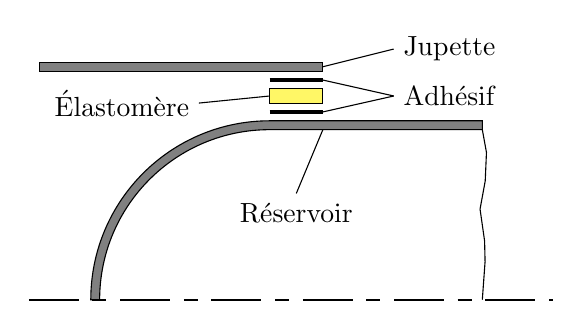
\begin{tikzpicture}[scale=0.9]

%Couleurs
\def \colelastomere{yellow!60}
\def \colreservoir{black!50}

%Dimentions du réservoir et de la jupette
\def \epaisseurreservoir{.125}
\def \ldroit{3}
\def \laxe{1.}
\def \tjupette{0.125}
\def \ljupette{4}
\def \rayonint{0.6*\ljupette}

%Définition de l'espace entre les éléments de la soudure
\def \espace{0.125}
\def \lsoudure{0.75}
\def \telastomere{0.2}

\tikzstyle{loosely dashed}=      [dash pattern=on 18pt off 5pt on 5pt off 5 pt]

%paroi du réservoir
\draw[black,fill=\colreservoir] (0,\rayonint) arc (90:180:\rayonint) -- ++ (- \epaisseurreservoir,0) arc (180:90:\rayonint+\epaisseurreservoir) -- ++ (\ldroit,0) -- ++ (0,-\epaisseurreservoir) -- cycle; 
\draw[black,decorate,decoration=random steps] (\ldroit,\rayonint) -- ++ (0,-\rayonint);

%Axe
\draw[black,thick,loosely dashed] (-\rayonint-\laxe,0) -- ++ (\rayonint+\ldroit+2*\laxe,0);

%Éléments chauffants
\draw[black,very thick] (0,\rayonint+\epaisseurreservoir+\espace) -- ++(\lsoudure,0);
\draw[black,very thick] (0,\rayonint+\epaisseurreservoir+3*\espace+\telastomere) -- ++(\lsoudure,0);

%Élastomère
\draw[black,fill=\colelastomere] (0,\rayonint+\epaisseurreservoir+2*\espace) -- ++(\lsoudure,0) -- ++(0,\telastomere) -- ++ (-\lsoudure,0) -- cycle;

%Jupette
\draw[black,fill=\colreservoir] (\lsoudure,\epaisseurreservoir+4*\espace+\telastomere+\rayonint)  -- ++ (-\ljupette,0) -- ++ (0,\tjupette) -- ++(+\ljupette,0)  -- cycle; 

%Identification
\draw[black,thin] (\lsoudure,\epaisseurreservoir+4*\espace+\telastomere+\rayonint+0.5*\tjupette) -- ++ (1,2*\espace) node[right] {Jupette};

\draw[black,thin] (\lsoudure,\epaisseurreservoir+3*\espace+\telastomere+\rayonint) -- ++ (1,-\espace-0.5*\telastomere) ;

\draw[black,thin] (0,\epaisseurreservoir+2*\espace+0.5*\telastomere+\rayonint) -- ++ (-1,-0.5*\telastomere) node[left] {Élastomère};

\draw[black,thin] (\lsoudure,\epaisseurreservoir+\espace+\rayonint) -- ++ (1,\espace+0.5*\telastomere) node[right] {Adhésif};

\draw[black,thin] (0.25*\ldroit,\rayonint) -- ++ (-0.5*\lsoudure,-0.375*\rayonint) node[below] {Réservoir};

%\node[inner sep=0pt] (SaturnV) at (9,2)
%{\includegraphics[width=.5\textwidth]{SaturnV_stage2.pdf}};
%
%\node (a) at (1,-3) {a)};
%\node (b) at (9,-3) {b)};
%
%\draw[red,very thick] (6.6,1) ellipse [x radius=1.5,y radius=0.4];
%\draw[red,very thick] (6.6,3.9) ellipse [x radius=1.5,y radius=0.4];

\end{tikzpicture}
	} \qquad
	\subfigure[]
	{\label{fig:schema_jonction_b}
		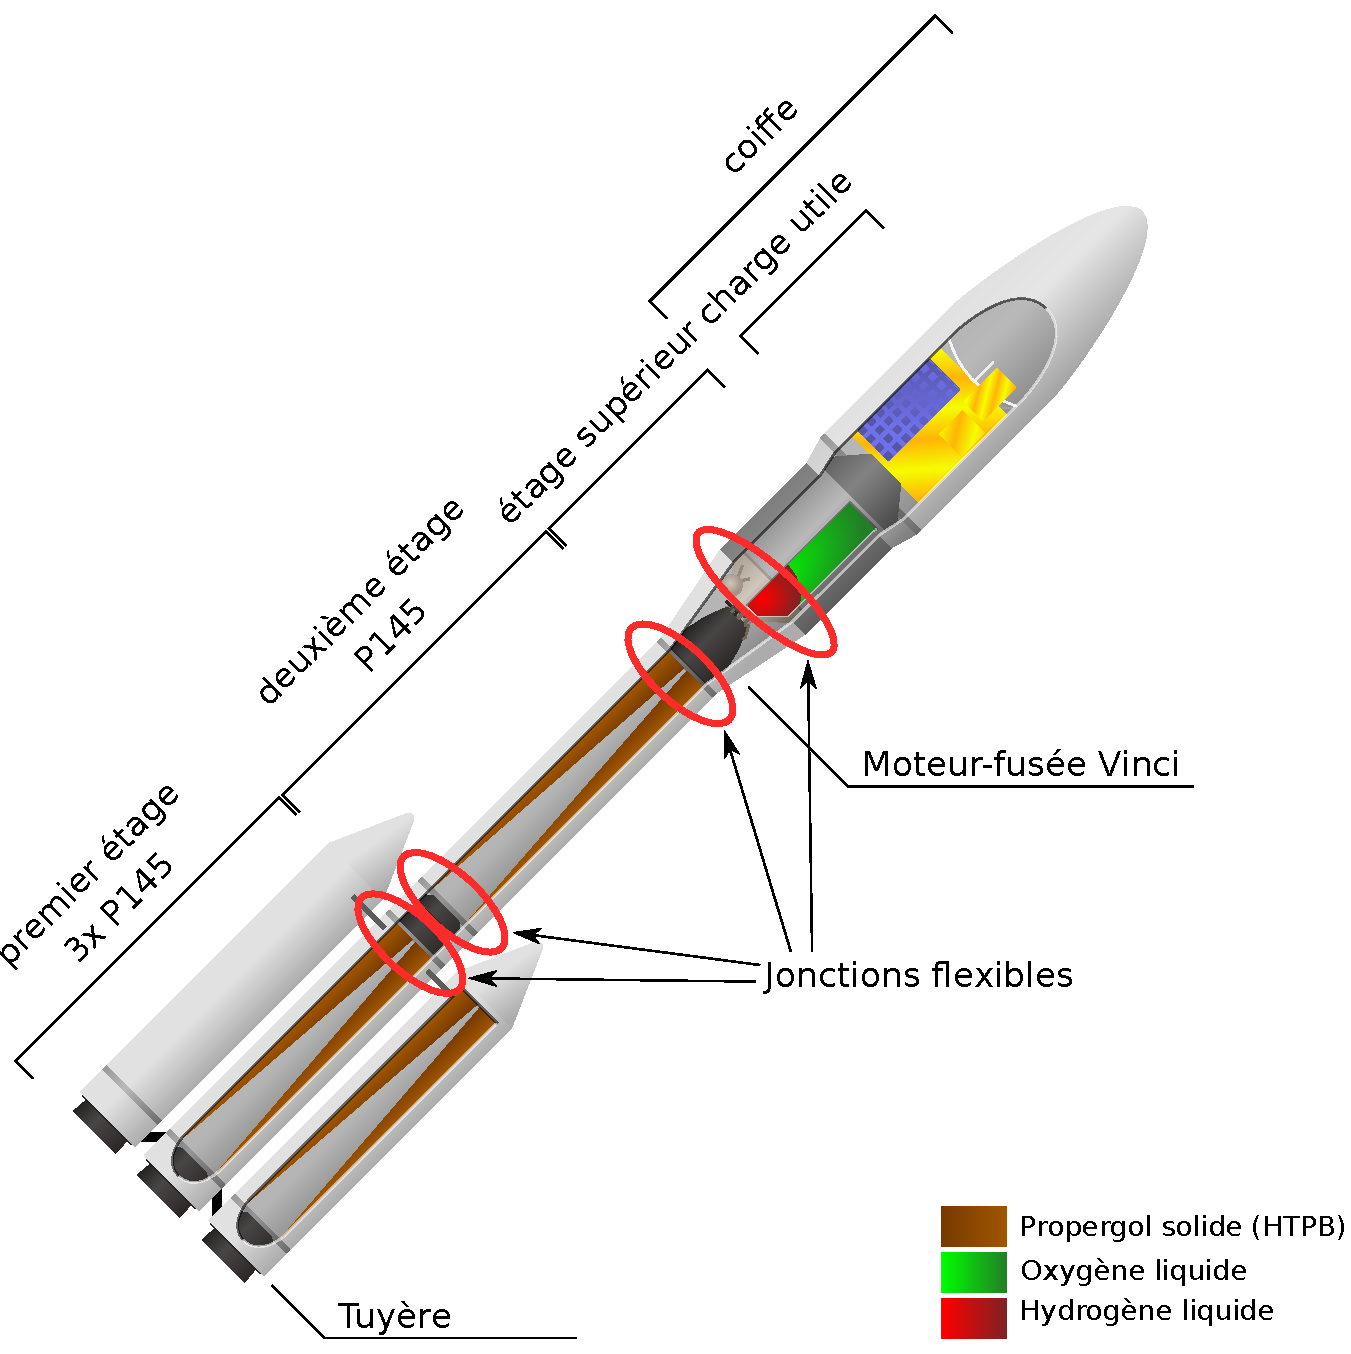
\includegraphics[width=0.45\textwidth]{Ariane_6_PPH_cutaway.pdf}
	}
	\caption{a) Schéma de la jonction flexible entre le réservoir et la jupette, b) emplacement des jonctions sur la fusée Ariane 6 (adaptée de \cite{Wikipedia:Ariane6}, sous licence Creative Commons)}
	\label{fig:schema_jonction}
\end{figure}

Une solution initiale employant des colles structurelles et un élastomère réticulé permettait d'atteindre les requis de performance pour les lanceurs fabriqués en composites thermodurcissables. 
En raison de problèmes de sensibilité environnementale lors de la préparation des joints et de longs temps de mise en œuvre, ArianeGroup a décidé d'explorer la possibilité de passer aux composites à matrice thermoplastique. 
Tout d'abord, cette transition leur permettra d'accélérer les cadences de production et de tirer profit des propriétés des composites à matrice thermoplastique telles que leur plus grande résistance aux impacts et, dans certains cas, aux solvants. 
Ensuite, cette conversion leur permettra d'augmenter la robustesse du joint et d'éviter des problèmes liés au collage tels que de longs temps de réticulation et une grande sensibilité à la préparation des surfaces et aux contaminants. 
Afin de compléter cette transition vers des structures en composites à matrices thermoplastiques, il est nécessaire de développer une nouvelle solution. 

L'objectif général des travaux présentés dans le cadre de cette thèse est de développer un procédé de soudage par résistance utilisant un nanocomposite conducteur comme élément chauffant pour joindre un adhérent en composite thermoplastique et un élastomère thermoplastique. 

%%
%%  CONCEPTS DE BASE / BASIC CONCEPTS
%%
%\section{Concepts de base}


\section{Éléments de la problématique}

La production d'une jonction flexible entre des adhérents en composite thermoplastique nécessite l'obtention de soudures multiples avec des matériaux aux propriétés très différentes. 
Sur le plan des concepts, le processus de soudage s'apparente aux processus de formation des lignes de soudures lors de la fabrication par injection de pièces en polymère ou lors de l'injection subséquente d'un autre polymère pour produire un surmoulage. 

Dans un premier temps, il sera nécessaire d'explorer les concepts associés au soudage tels que l'autohésion et la diffusion des chaines de polymères. 
Une recension des écrits concernant le soudage des composites thermoplastiques permettra de bien cibler les paramètres clés à optimiser et d'établir des comparatifs avec les résultats qui sont obtenus. 

En second lieu, pour la jonction avec l'élastomère, peu de réponses existent déjà dans la littérature scientifique.
Il est donc nécessaire de développer une approche expérimentale progressive et méthodique pour résoudre cette portion du problème. 

%%
%% PLAN DU MEMOIRE / THESIS OUTLINE
%%
\section{Plan de la thèse}  % 0.5 page

À la suite de cette introduction, le chapitre \ref{sec:RevLitt} présentera l'ensemble des connaissances contenues dans les travaux publiés ayant rapport à la production de jonctions flexibles par soudage résistif. 
Cette section discutera tout d'abord des matériaux composites, des techniques de mise en forme ainsi que des paramètres propres au soudage. S'ensuivra une section à propos des nanocomposites conducteurs d'électricité. Le chapitre se terminera avec une courte discussion sur les élastomères thermoplastiques.

Par la suite, au chapitre \ref{sec:Objectifs}, une analyse objective des écrits publiés permettra de cerner les limites de la connaissance actuelle et de définir plus particulièrement les objectifs de recherche. 

Les chapitres \ref{sec:Theme1} à \ref{sec:Theme3} quant à eux présenteront les principaux travaux réalisés dans le cadre de cette thèse. 
Les sujets de ces chapitres seront directement en lien avec les objectifs précédemment présentés. 

Le chapitre \ref{sec:Discussion} traitera de travaux ayant été réalisés dans le cadre de cette thèse, mais ne figurant pas dans les thématiques abordées dans le cadre des travaux principaux présentés aux chapitres \ref{sec:Theme1} à \ref{sec:Theme3}.  

Le chapitre \ref{sec:Contributions} mettra en valeur les contributions originales de ces recherches. 
Ce chapitre présentera une synthèse des principaux résultats positifs et négatifs. 
Il démontrera comment les travaux réalisés durant cette thèse ont permis d'avancer le niveau de connaissance par rapport au soudage par résistance et à la production de jonction flexible. 
Ce chapitre portera également un regard critique sur les résultats obtenus en recherchant les limites d'applicabilité des nouvelles connaissances et se conclura par la suggestion de pistes pour de nouveaux projets de recherche. 
       % Introduction au sujet de recherche.
\selectlanguage{french}
\Chapter{REVUE DE LA LITTÉRATURE}\label{sec:RevLitt}

\section{Matériaux composites}

Les matériaux structurels peuvent être divisés en 4 grandes classes: les métaux, les polymères, les céramiques et les verres, et les composites \cite{ashby2018materials}. 
Un matériau composite est un assemblage solide d'au moins deux phases hétérogènes aux propriétés différentes dans le but d'obtenir un matériau aux propriétés différentes des phases isolées. 
Les phases restent distinctes et séparées dans le matériau final \cite{Wikipedia_mat_comp}. 
Ces mélanges permettent d'obtenir des matériaux sur mesure avec des propriétés ajustées selon le besoin de l'application. 
Il est ainsi possible de produire des matériaux plus légers, plus résistants aux sollicitations mécaniques, plus conducteurs, plus rigides, avec une meilleure tenue en température ou toute autre propriété visée. 

Les matériaux composites modernes sont composés d'une matrice polymérique, métallique ou céramique, et d'un renfort sous forme de particules ou de fibres. 
Les matériaux composites sont divisés en catégories selon la nature des phases en présence. 
Si on exclut le béton, les composites à matrice polymérique représentent la majorité des composites produits industriellement. 
Comme matériaux de renforts utilisés, on retrouve une majorité de composites de fibres inorganiques telles que les fibres de verre ou les fibres de carbone et, dans une plus faible proportion, de composites à base de fibres polymériques telles que l'aramide (ex. : Kevlar, Nomex, etc.) ou le polyéthylène à très grande masse moléculaire (ex. : Dyneema, Spectra, etc. ). 
Ces fibres sont sélectionnées pour leur très grande résistance spécifique et leur module de Young élevé. 
Les composites modernes utilisent une grande variété de fibres aux propriétés variées (Fig.~\ref{gibson2}). 
Les fibres sont disponibles commercialement sous la forme de fibres courtes, de rouleaux de fibres unidirectionnelles ou de toiles tissées. 

\begin{figure}
	\centering
	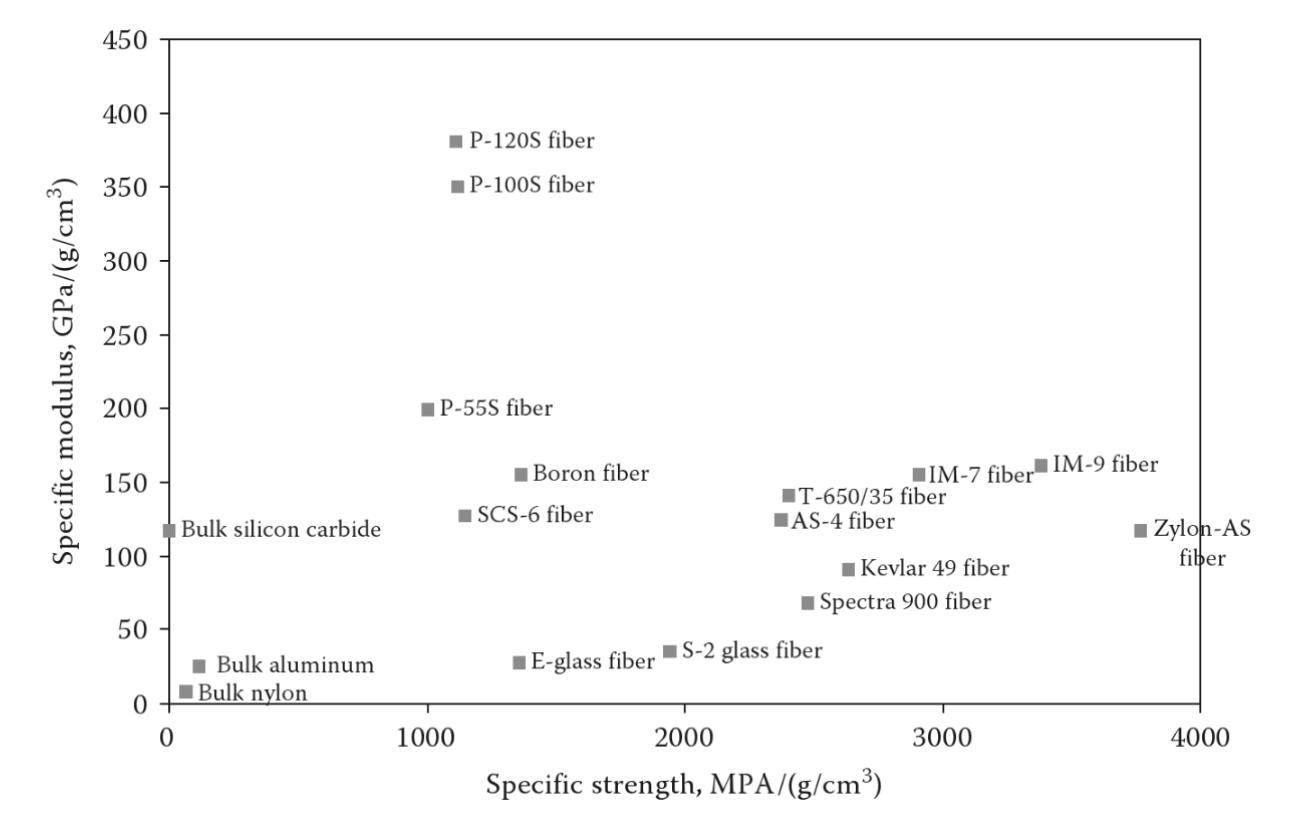
\includegraphics[width=0.9\textwidth]{gibson2}
	\caption{Comparaison des fibres utilisées pour les composites modernes (tirée de \cite{Gibson2011}, reproduction avec autorisation)}
	\label{gibson2}
\end{figure}

En ce qui concerne la matrice, les développements initiaux des composites à matrice polymérique ont été réalisés avec des polymères thermodurcissables. 
Ces derniers ont été favorisés au départ en raison de la possibilité de les employer à l'état liquide à pression ambiante, avant la polymérisation, pour imprégner les fibres \cite{Chatain2015}. 
C'est pour cette raison qu'encore aujourd'hui les composites à matrice thermodurcissable occupent la majorité du marché des composites à matrice polymérique. 

\FloatBarrier
\subsection{Performances}

Les performances mécaniques des composites proviennent de la combinaison des fibres et de la matrice qui les supportent. 
Malgré leur très faible densité, les fibres possèdent des modules d'élasticité et des résistances à la traction très élevés en comparaison avec les propriétés des matériaux traditionnels tels que les aciers alliés ou l'aluminium \cite{Hull2001}.
Cependant, les fibres offrent très peu de résistance à la compression dans leur axe en raison de leur géométrie et sont incapables de redistribuer la charge entre elles sans l'aide d'un support. 
En combinant les fibres rigides à une matrice leur offrant un support et permettant de transférer les charges, on obtient un matériau aux propriétés fortement dépendantes de l'orientation. 
Les matériaux composites à fibres continues sont très résistants face aux sollicitations orientées selon le sens des fibres, mais ils sont très sensibles aux sollicitations en dehors de cet axe. 
Une déviation de plus de 5° dans l'orientation de la force produit une forte dégradation des performances \cite{Hull2001}. 
Il est donc important lors de la fabrication de conserver l'orientation des fibres afin d'obtenir des propriétés mécaniques optimales. 
De plus, même si chaque pli de composite est sensible aux sollicitations en dehors de son axe principal, il est possible de superposer une série de plis avec différentes orientations afin que le laminé composé possède de meilleures propriétés selon certains axes définis. 

En ce sens, le développement de pièces en composite doit prendre en compte la nature directionnelle des propriétés des composites, puisqu'un impact sur les résultats sera observable lors de l'évaluation de la résistance aux chargements mécaniques. 
Néanmoins, la faible densité des matériaux composites permet de réduire le poids global des structures en maintenant les niveaux de performances. 

Un autre avantage de la nature hétérogène des composites réside dans leur résistance à la propagation des fissures. 
Contrairement aux métaux qui n'offrent pas de frontières à la propagation des fissures, la présence de fibres au travers des fissures permet de maintenir une intégrité mécanique des pièces. 
Tandis que la matrice polymérique peut fissurer et se déformer pour absorber une partie de l'énergie de déformation, les fibres résistent encore un moment en ralentissant la vitesse de propagation des fissures \cite{Hull2001}. 

\subsection{Composites à matrice thermoplastique}

Les composites à matrice thermoplastique ont commencé à être considérés sérieusement durant les années 1980 pour améliorer la durabilité et la résilience aux impacts à basse vitesse des composites \cite{asmhandbook21}. 
Même si le marché continue d'utiliser en grande quantité les matrices thermodurcissables, les compagnies aéronautiques telles qu'ArianeGroup convertissent de plus en plus leurs procédés de fabrication pour utiliser les composites thermoplastiques. 
Du côté de l'automobile également, afin de rencontrer les cibles de consommation de carburant américaines et européennes, les manufacturiers intègrent un volume croissant de composites à leurs produits afin d'en réduire la masse. 
Les composites à matrice thermoplastique occupent un rôle central dans cette transition \cite{CompositesWorld2019_market2020}. 

En plus de leur plus grande résilience, les composites à matrice thermoplastique sont moins sensibles aux contaminants et à leur environnement que les composites à matrice thermodurcissable, et ce, autant durant leur service ainsi que lors de leur mise en forme. 
Puisque les composites à matrice thermoplastique sont déjà totalement polymérisés, la présence de solvants ou de graisse n'affecte pas le processus de polymérisation \cite{cogswell1992}. 
Les composites thermoplastiques ont également une plus faible sensibilité à l'humidité.  
La polymérisation complète des matrices thermodurcissables nécessite des durées de plusieurs heures suivies de traitements de cuisson, souvent à l'autoclave, pour terminer la réaction. 
La mise en forme à l'autoclave des composites à matrice thermodurcissable, pour le domaine de l'aéronautique, nécessite une grande quantité d'énergie et d'espace. 
Les dimensions des autoclaves doivent être suffisantes pour contenir par exemple des pièces du fuselage ou encore des segments d'ailes. 
Même si la puissance requise pour chauffer une pièce en composites à matrice thermoplastique est plus élevée lors de sa mise en forme, la courte durée de cette opération réduit grandement les besoins en énergie comparativement à celle nécessaire à la cuisson des composites thermodurcissables sur une longue durée. 
L'élimination du temps nécessaire à la polymérisation et à la cuisson permet de raccourcir grandement les temps de production et ainsi de multiplier la cadence de production. 
Finalement, puisque les thermoplastiques peuvent être refondus, il est possible de réparer les composants à la suite de fissures n'ayant pas cassé les fibres ou encore de les recycler en fin de vie utile. 

\subsection{Mise en forme}

Contrairement aux composites à matrice thermodurcissable qui doivent être moulés directement à leur forme finale, les composites à matrice thermoplastique ont la possibilité d'être fondus à plusieurs reprises. 
Les différentes méthodes de mise en forme des composites à matrice thermoplastique sont principalement des variations quant aux méthodes de chauffe et de mise en place des matériaux. 

Les principales méthodes de fabrication sont l'enroulement filamentaire, la déposition de ruban, le moulage par compression dans un moule rigide ou flexible, la mise en forme par diaphragme dans une presse ou en autoclave, l'emboutissage, le laminage, l'extrusion par tirage et le transfert de résine \cite{asmhandbook21, campbell2003}.  

La sélection d'une méthode de mise en forme repose sur le type de géométrie à réaliser, le type de fibre qui doit être utilisé et la nature du polymère. 
Par exemple, les procédés d'enroulement filamentaire ou encore de mise en forme par déposition de ruban ne permettent pas de fabriquer des composites avec des toiles tissées. 
Ces procédés ont la particularité d'employer des rubans de fibres unidirectionnelles déposés de façon linéaire. 
Il est cependant possible de changer la direction de déposition lors des passages subséquents pour obtenir un composite avec des couches orientées différemment. 
Dans le même ordre d'idées, le procédé de transfert de résine ne peut être appliqué qu'aux thermoplastiques pouvant être injectés sous forme de monomères qui polymériseront ensuite dans la pièce tels que le polyamide-6 anionique (APA-6) \cite{Rijswijk2006} ou certaines résines acryliques récemment développées \cite{Penumadu2019,Murray2019}. 

Notre partenaire industriel a développé un procédé d'enroulement filamentaire avec un chauffage par laser pour la fabrication des réservoirs \cite{Krzeminski2014}. 
Le procédé développé pour joindre les plaques de composites à l'élastomère devra donc être compatible avec ce type de pièces. 

\subsection{Jonction des pièces en composite}

En raison de la nature directionnelle des propriétés des matériaux composites, la jonction effectuant le transfert de charge entre les composants mécaniques ne peut être conçue comme pour les matériaux isotropes. 
Les jonctions entre pièces de composites présentent des discontinuités dans la structure même du matériau. 
De façon plus prononcée que pour les pièces réalisées à l'aide de matériaux isotropes, les jonctions représentent des zones critiques lors de la conception de structures en composite. 
En raison de la flexibilité des processus de mise en forme, il est possible de réduire le nombre de jonctions en produisant des composants aux géométries plus complexes. 
Parfois, une seule pièce en composite peut remplacer tout un assemblage de pièces et ainsi sauver des couts \cite{KarenMas_CW2004}. 

Les méthodes employées pour réaliser des jonctions entre les pièces en composite peuvent être classifiées en deux grandes catégories. 
\begin{enumerate}
	\item Les jonctions ponctuelles qui causent un transfert de charge qui peut être localisé en un point. 
	Cette catégorie englobe les liaisons avec des rivets et le soudage point à point. 
	\item Les méthodes permettant plutôt un transfert de charge sur une surface. 
	Cette seconde catégorie englobe des procédés tels que le collage ou le soudage. 
\end{enumerate}
Afin de favoriser un bon transfert des charges mécaniques, pour les applications structurelles où les pièces ne peuvent pas être combinées afin d'éliminer les jonctions, les joints de la seconde catégorie sont fortement conseillés \cite{campbell2003}. 

Les composites thermodurcissables sont limités dans les options d'assemblage. 
Il est possible de les assembler par co-consolidation, collage ou assemblage mécanique à l'aide de boulons ou de rivets.
Dans le cas des composites à matrice thermoplastique, un plus large éventail de méthodes de soudage s'ajoute aux méthodes déjà disponibles pour les composites thermodurcissables \cite{campbell2003}. 
Puisque le collage de composites à matrice thermoplastique produit des joints moins résistants que pour les composites à matrice thermodurcissable --- en raison de la nature des polymères \cite{campbell2003} --- et que les procédés de soudage sont moins sensibles aux contaminants, ces derniers sont préférés pour l'assemblage des composants. 

\section{Compatibilité des mélanges de polymères}

Il est possible de valider la compatibilité des composants d'un mélange de polymères avec la théorie de Flory-Huggins, développée par Flory \cite{Flory1941} et Huggins \cite{Huggins1941}. 
Ce modèle basé sur le comportement thermodynamique des solutions polymères prend en compte l'effet de la longueur des chaines de polymères dans le calcul de l'entropie de mélange et du changement de l'énergie libre de Gibbs ($\Delta G_m$). 
À partir de la constante universelle des gaz parfaits ($R_m$), de la température ($T$), des nombres de moles ($n_1$ et $n_2$) et des fractions volumiques ($\phi_1$ et $\phi_2$) des composants, on peut évaluer la relation entre la variation de l'énergie libre de Gibbs et le paramètre de Flory ($\chi_{12}$), définissant l'affinité entre les composants, à l'aide de l'équation suivante.

\begin{equation}
\Delta G_m = R_m T \left[ n_1 \ln \phi_1 + n_2 \ln \phi_2 + n_1 \phi_2 \chi_{12} \right]
\end{equation}

La théorie de Flory-Huggins a initialement été développée pour les solutions de polymères dans un solvant, mais a été étendue à des mélanges binaires de polymères et d'autres combinaisons pouvant inclure des solvants \cite{Huggins1942a,Scott1949,Fredrickson1994c}. 
On peut également utiliser le paramètre de Flory pour étudier la compatibilité et le comportement des copolymères \cite{Scott1952c}. 
Des facteurs de corrections entropiques prenant en compte l'architecture des polymères (structure linéaire, à branches ou en étoile) et leur degré de conformation ont également été développés pour améliorer le modèle \cite{Fredrickson1994c}. 
Plus récemment, certains auteurs ont contesté la validité de ce paramètre pour proposer un nouveau critère ($g$) indépendant de la concentration et de la température \cite{Tambasco2006c,Higgins2010c,White2012c}. 

\section{Reptation des polymères thermoplastiques}

La reptation des chaines est un phénomène clé pour la compréhension de l'évolution du comportement mécanique des jonctions soudées. 
Pendant le procédé de soudage, lors de la mise en contact des faces à joindre, les chaines de polymères mobiles diffusent entre les pièces et on observe progressivement une homogénéisation de la soudure et la disparition de la frontière entre les pièces (Fig.~\ref{fig:polymer_diffusion}). 
Cette diffusion des chaines se produit principalement en deux étapes. 
\begin{enumerate}
	\item Développement du contact intime entre les adhérents.
	\item Interdiffusion des chaines au travers de l'interface.
\end{enumerate}

\begin{figure}[h]
	\centering
	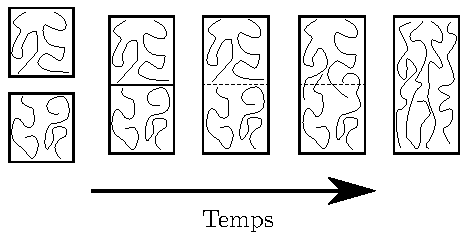
\includegraphics[scale=1.1]{welding_chain_diffusion.pdf}
	\caption{Diffusion des chaines de polymères durant le soudage : a) état initial, b) mise en contact des faces, c) formation du contact intime entre les faces, d) diffusion des chaines de polymères au travers de l'interface et e) disparition de l'interface. }
	\label{fig:polymer_diffusion}
\end{figure}

\FloatBarrier
Avant même que la diffusion des chaines ne puisse prendre place, les faces en contact doivent atteindre un état de contact intime. 
Durant cette étape, les surfaces se conforment les unes aux autres, mais la diffusion des chaines de polymères n'a pas encore débuté. 
La question de contact intime a été abordée très tôt dans le développement des composites à matrice thermoplastique en raison de la nécessité de consolider les couches lors de la fabrication des pièces. 
Les équations développées pour l'atteinte de cet état prennent en compte la rugosité de la surface à l'aide de paramètres géométriques ($a^*$ et $w^*$), la pression de contact ($P_{app}$) et la viscosité de la matrice polymérique ($\mu _{mf}$). 
Les premiers modèles simplifiaient la surface en une série de rectangles idéalisés d'aire constante, mais dont la hauteur et la largeur varient en fonction du temps \cite{Lee1987}. 
En intégrant la variation de la pression et de la viscosité sur le temps depuis la mise en contact ($t_c$), on arrive à l'équation suivante décrivant le degré de contact intime ($D_{ic}$) \cite{Mantell1992a} : 

\begin{equation}
D_{ic} \approx \frac{1}{w^*} \left[ a^* \int_{0}^{t_c} \frac{P_{app}}{\mu _{mf}} \, dt \right]^{\frac{1}{5}}
\label{eq:contact_intime}
\end{equation}

Les modèles basés sur des rectangles idéalisés sont incapables de prédire le comportement depuis des mesures directes de la rugosité des interfaces et nécessitent des paramètres d'ajustement obtenus à la suite d'essais en laboratoire \cite{Yang2001}. 
Une autre génération de modèles tente plutôt de représenter la surface comme une série de rectangles de tailles diverses parfois semblables à une fractale dont les propriétés peuvent être reliées à des mesures de rugosité des surfaces \cite{Yang2001,Yang2002}. 
Dans ces modèles, le polymère est écrasé jusqu'à ce que tous les rectangles d'aire constante forment une frontière unique. 
À partir de données de rugosité, Yang et Pitchumani ont pu établir un modèle montrant une évolution rapide du critère de contact intime suivi d'un ralentissement à l'approche du plein contact \cite{Yang2001}. 
Dans des conditions isothermes à \SI[locale=FR]{350}{\celsius} avec des pressions de 0,67 et \SI[locale=FR]{1,63}{\mega\pascal}, le contact intime est totalement atteint avec des temps respectivement de \SI[locale=FR]{100}{\second} et de \SI[locale=FR]{40}{\second} pour des laminés en Polyétheréthercétone (PEEK). 
Une hausse de la température ou de la pression diminue très rapidement le temps nécessaire pour atteindre la condition de contact intime \cite{Yang2002}. 

La seconde étape du développement de la jonction entre les pièces est l'interdiffusion des chaines au travers de l'interface. 
Ce phénomène se produit par un mouvement des chaines de polymères au travers de l'interface entre un même polymère ou des polymères compatibles \cite{Jud1981b}. 
La reconfiguration des chaines dans le polymère se produit par un phénomène de reptation et de mouvement brownien qui a été conceptualisé, pour les polymères fondus, assez tôt \cite{DeGennes1971,Edwards1978b,Klein1978,Daoud1979}. 
L'interdiffusion par transfert des chaines de polymères au travers de l'interface peut se produire lorsque des polymères amorphes compatibles sont chauffés au-dessus de leur température de transition vitreuse et qu'ils sont en contact \cite{Jud1981a,Prager1981a}. 
L'interdiffusion se produit par le mouvement stochastique de l'extrémité des chaines entre deux pièces en contact et entraine une reconfiguration des chaines. 
Cette dernière entraine également la formation d'enchevêtrements de chaines au travers de l'interface \cite{Wool1983}. 
La diffusion des chaines entraine la disparition progressive de la démarcation entre les pièces en contact. 
Le temps requis pour éliminer une fissure a été défini comme étant le temps nécessaire pour que les molécules adjacentes à la fissure diffusent à mi-chemin \cite{Prager1981a}.
Selon la nature du polymère, son poids moléculaire, la température et la pression, le processus d'interdiffusion peut se produire en quelques minutes ou peut nécessiter plusieurs heures voire même des jours \cite{Prager1981a}. 
On nomme le temps de reptation ($t_r$) le temps que prend une chaine de polymère pour quitter totalement sa configuration d'origine et atteindre une nouvelle configuration géométrique. 
Dans le cas d'une soudure où l'ensemble de la surface n'est pas à une température constante, l'interdiffusion commence à se produire progressivement dans les sections ayant déjà atteint le contact intime. 

Le temps de reptation est un paramètre clé pour évaluer la vitesse du phénomène de diffusion des chaines de polymères. 
Pour les polymères amorphes, on peut citer les travaux de Wool \cite{Wool1983,Wool1989}. 
Ces derniers traitent de l'évolution des propriétés mécaniques durant la phase de transition vers la diffusion complète des chaines de polymères en condition isotherme. 
Il dénote entre autres que la quantité d'énergie nécessaire pour séparer des interfaces dépend de quatre paramètres : \begin{inparaenum}[(1)]
	\item le temps ($t$), 
	\item la température ($T$), 
	\item la pression ($P_{app}$) et
	\item la masse moléculaire ($M$). 
\end{inparaenum}
Ce dernier paramètre est directement lié au temps de reptation tel que \cite{DeGennes1971}: 

\begin{equation}
t_r \approx M^3
\end{equation}

Wool introduit également plusieurs relations dynamiques décrivant le déplacement des chaines de polymères en fonction du temps \cite{Wool1983,Wool1989}. 
Une première relation introduite est la longueur moyenne des chaines mineures ayant traversé l'interface en fonction du temps ($l(t)$). 
Les chaines mineures sont définies comme étant la section des chaines ayant quitté le tube initial dans lequel la chaine complète était initialement contenue. 
Les chaines mineures débutent depuis l'extrémité des chaines et croissent progressivement tout au long de la chaine jusqu'à se rejoindre au milieu. 
On peut conceptualiser le mouvement des chaines mineures comme étant un mouvement de marche aléatoire. 
À partir de la longueur moyenne des chaines mineures, la distance moyenne d'interpénétration des monomères en fonction du temps ($\chi(t)$) peut être évaluée. 
Ces deux paramètres évoluent selon deux échelles de temps distinctes. 

\begin{equation}
l(t) \propto t^{1/2} M^{-1/2}
\end{equation}

\begin{equation}
\chi(t) \propto t^{1/4} M^{-1/4}
\end{equation}

L'impact de la température sur le temps de reptation peut être évalué à l'aide d'une équation d'Arrhenius où les paramètres $A_r$ et $B_r$  doivent être évalués expérimentalement \cite{Bastien1991,Ageorges1998}. 

\begin{equation}
t_r = B_r \, exp \left( \frac{A_r}{T} \right)
\end{equation}

En condition isotherme et pour un temps de reptation donné, la résistance de la soudure ($\sigma$) évolue, en fonction du temps ($t$), de façon non linéaire où le degré d'interdiffusion ($D_{h}$) est estimé tel que \cite{F.Yang2002} : 

\begin{equation}
D_h \left( t \right) = \frac{\sigma}{\sigma_{\infty}} \propto \left( \frac{t}{t_r} \right)^{1/4}
\end{equation}

Autrement, en définissant la résistance de la soudure à un temps infini ($\sigma_{\infty}$) telles que \cite{Wool1983} :

\begin{equation}
\sigma_{\infty} \propto M^{1/2}
\end{equation}

et en observant que la résistance de la soudure évolue, pour des temps inférieurs au temps de reptation, telle que \cite{Wool1983} :

\begin{equation}
\sigma \propto \left( \frac{t}{M} \right) ^{1/4}
\end{equation}

on obtient, pour la période où le temps ($t$) est inférieur au temps de reptation ($t_r$), une estimation de l'évolution de la résistance de la soudure \cite{Wool1983} : 

\begin{equation}
\frac{\sigma}{\sigma_{\infty}} \propto t^{1/4} M^{-3/4}
\end{equation}

D'autres chercheurs (tels que Bastien, Yang et Ageorges) ont développé des équations décrivant l'évolution d'une soudure pour tenir compte de conditions non isothermes en discrétisant les phénomènes de contact intime et d'interdiffusion en fonction du temps  \cite{Bastien1991,F.Yang2002,Ageorges1998}. 

En se basant sur des données expérimentales provenant d'essais en condition isotherme réalisés dans le but d'estimer les temps de reptation en fonction de la température, Bastien a pu prévoir la résistance obtenue après un soudage en condition non isotherme, pour des jonctions entre des adhérents en polyétherimide (PEI) \cite{Bastien1991}. 
Les modèles développés par Bastien utilisent des critères développés par Wool, soit la longueur moyenne des chaines mineures ayant traversé l'interface en fonction du temps ($l(t)$) et la distance moyenne d'interpénétration des monomères en fonction du temps ($\chi(t)$) \cite{Wool1983}. 
Le modèle de Bastien basé sur la distance moyenne d'interpénétration obtient des temps de reptation du même ordre de grandeur que les temps de reptation évalués expérimentalement (Tab. \ref{tab:temps_de_reptation_Bastien}). 
Le modèle basé sur la longueur des chaines mineures ayant traversé l'interface donne des temps de reptation qui divergent des mesures expérimentales. 
Les résultats obtenus avec le paramètre d'interpénétration ont des marges d'erreur d'environ 20\%, mais confirment la possibilité d'obtenir des soudages de qualité avec des temps de mise en forme courts.

\begin{table}[h]
	\centering
	\caption{Évaluation expérimentale des temps de reptation et comparaison avec les résultats des modèles (traduit de \cite{Bastien1991})}
	\label{tab:temps_de_reptation_Bastien}
	\begin{tabular}{@{}lcccc@{}}
		\toprule
		& \multicolumn{1}{l}{} &          \multicolumn{3}{c}{Temps de reptation}          \\
		Type d'essai         &          Température &      Résultats &          Critère &  Critère \\
		&                      &   expérimentaux & $\chi(t)$ & $l(t)$ \\
		&      [\si{\celsius}] & [\si{\second}] &   [\si{\second}] &       [\si{\second}] \\ \midrule
		Moulage à la presse  &                  230 &        300 880 &          510 000 &            5 400 000 \\
		Essais de fluage     &                  250 &           4 800 &             5 446 &               99 131 \\
		Mesures en rhéologie &                  270 &          1 - 8 &               81 &                 2 437 \\ \bottomrule
	\end{tabular}%
\end{table}

Un modèle subséquent est parvenu à améliorer les prédictions de temps d'interdiffusion pour les conditions de variations rapides de température et permet d'évaluer avec plus de précision l'état d'une interface soudée \cite{F.Yang2002}. 
Les équations de développement du contact intime et du phénomène d'interdiffusion ont été mises en application avec des résultats probants pour élaborer une fenêtre d'opération pour le soudage de composites à matrice thermoplastique~\cite{Ageorges1998}. 

La littérature n'est pas aussi développée en ce qui concerne les thermoplastiques semi-cristallins. 
Cependant, certains travaux ont permis de démontrer l'importance de la co-cristallinité et de la température sur la possibilité d'obtenir un soudage entre thermoplastiques semi-cristallins  \cite{Xue1998,Smith2001}. 
Le taux de cristallinité a également un grand impact sur la possibilité de souder des pièces. 
Les cristaux présents dans les adhérents semi-cristallins affectent la facilité avec laquelle les chaines de polymères peuvent migrer à l'interface \cite{Jarrousse2004}. 
Un taux de cristallinité élevé crée des entraves au déplacement des chaines en dessous de la température de fusion tandis qu'un échantillon faiblement cristallin possède des zones amorphes qui peuvent migrer et interdiffuser sous la température de fusion. 
Lors de la fusion des cristaux, la possibilité de former des cristaux en co-cristallinité qui unissent les deux phases est un facteur important à considérer \cite{Smith2001,Zanetto2001}. 
Plus la température est élevée, plus la soudure pourra se développer jusqu'à atteindre la résistance normale du polymère. 

\section{Soudage des composites à matrice thermoplastique}

Les composites à matrice thermoplastique, contrairement aux composites à matrice thermodurcissable, ont la possibilité d'être fondus pour modifier leur forme. 
Cette particularité leur permet également d'être pliés ou emboutis pour former des géométries plus complexes à partir de plaques planes ou encore de les assembler par soudage. 
Lors du soudage, les pièces à joindre sont fondues ou chauffées à l'interface, pressées ensemble et finalement consolidées pour obtenir une seule pièce continue. 
L'absence de transition dans le matériau a ouvert la porte à la certification des pièces obtenues pour le domaine de l'aviation \cite{Gardiner2018}. 

\begin{figure}[h]
	\centering
	\resizebox{0.75\textwidth}{!}{
		\tikzset{
	basic/.style  = {draw, text width=6cm, drop shadow, rectangle},
	root/.style   = {basic, rounded corners=2pt, thin, align=center,
                   fill=gray!30},
	level 2/.style = {basic, rounded corners=5.5pt, thin,align=center, fill=gray!10,
                   text width=8em},
	level 3/.style = {basic, thin, align=left, fill=white, text width=6.em}
}


\begin{tikzpicture}[
	level 1/.style={sibling distance=45mm},
	edge from parent/.style={->,draw},
	>=latex,
	scale=0.9,
	level distance=1.8cm]

% root of the the initial tree, level 1
\node[root] {Procédés de soudage}
% The first level, as children of the initial tree
	child {node[level 2] (c1) {Chauffage en volume}}
	child {node[level 2] (c2) {Chauffage par friction}}
	child {node[level 2] (c3) {Chauffage électromagnétique}}
	child {node[level 2] (c4) {Soudage en deux étapes}};

% The second level, relatively positioned nodes
\begin{scope}[every node/.style={level 3}]
\node [below of = c1, xshift=5pt, yshift=-11pt] (c11) {Co-consolidation};
\node [below of = c11, yshift=-6pt] (c12) {Adhésifs à chaud};
\node [below of = c12, yshift=-13pt] (c13) {Assemblage avec film \mbox{amorphe}};

\node [below of = c2, xshift=5pt, yshift=-11pt] (c21) {Soudage par friction};
\node [below of = c21, yshift=-6pt] (c22) {Soudage par vibration};
\node [below of = c22, yshift=-6pt] (c23) {Soudage par ultrasons};

\node [below of = c3, xshift=5pt, yshift=-11pt] (c31) {Soudage par induction};
\node [below of = c31, yshift=-6pt] (c32) {Soudage par micro-onde};
\node [below of = c32, yshift=-6pt] (c33) {Soudage \mbox{diélectrique}};
\node [below of = c33, yshift=-6pt] (c34) {Soudage \mbox{par résistance}};

\node [below of = c4, xshift=5pt, yshift=-17pt] (c41) {Soudage par plaque \mbox{chauffante}};
\node [below of = c41, yshift=-14pt] (c42) {Soudage au gaz chaud};
\node [below of = c42, yshift=-6pt] (c43) {Soudage \mbox{infrarouge}};
\node [below of = c43, yshift=-6pt] (c44) {Soudage au laser};
\end{scope}

% lines from each level 1 node to every one of its "children"
\foreach \value in {1,2,3}
	\draw[->] (c1.195) |- (c1\value.west);

\foreach \value in {1,...,3}
	\draw[->] (c2.195) |- (c2\value.west);

\foreach \value in {1,...,4}
	\draw[->] (c3.195) |- (c3\value.west);

\foreach \value in {1,...,4}
	\draw[->] (c4.195) |- (c4\value.west);
\end{tikzpicture}
}
	\caption{Procédés de soudage (adaptée de \cite{Ageorges2001a}, reproduction avec autorisation)}
	\label{fig:arbre_procédé_soudage}
\end{figure}

\FloatBarrier
De nombreux procédés existent pour souder des polymères. 
La source de chaleur employée est généralement l'élément différenciateur entre les procédés (Fig.~\ref{fig:arbre_procédé_soudage}). 
Il existe les procédés de chauffe en volume où les composants de l'assemblage sont chauffés en totalité. 
Ces procédés peuvent être réalisés entre autres dans un autoclave ou une presse chauffante. 
Un exemple de méthode de soudage dans cette catégorie est le procédé Thermabond qui utilise des films de polymères amorphes comoulés à la surface des adhérents en polymère semi-cristallin \cite{Smiley1991a}. 
L'assemblage est chauffé dans une plage de température permettant la soudure du polymère amorphe, mais évitant la fonte du polymère semi-cristallin (Fig.~\ref{fig:thermabond_process}). 
En raison de leur grande demande énergétique, les procédés de chauffe en volume sont généralement considérés comme étant peu efficaces. 

\begin{figure}[h]
	\centering
	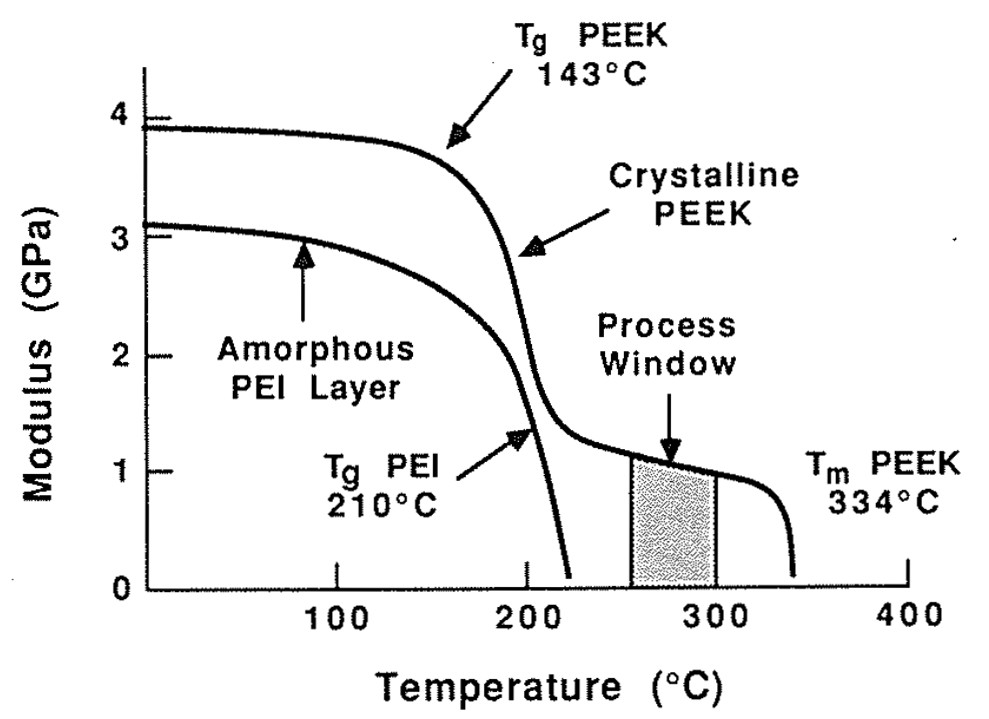
\includegraphics[width=0.55\textwidth]{Thermabond_Bastien1991.jpg}
	\caption{Modules du PEEK et du PEI illustrant la plage de température du procédé de soudage avec un film amorphe (tiré de \cite{Bastien1991}, reproduction avec autorisation)}
	\label{fig:thermabond_process}
\end{figure}

\FloatBarrier
Une seconde famille regroupe les procédés produisant un chauffage par friction, vibration ou ultrasons \cite{Bates2007d,Levy2014}. 
À l'aide d'un mouvement alternatif rapide, la friction entre les composants produit un échauffement local. 
Ce même effet peut également être obtenu à l'aide d'ultrasons en raison de l'hystérésis thermomécanique des matériaux. 
Ces méthodes pour joindre des composants sont rapides, mais peuvent induire un déplacement des fibres. 
Également, malgré ses très bonnes performances mécaniques \cite{Villegas2016}, l'application du soudage par ultrasons peut être complexe pour les jonctions sur de longues distances lorsqu'une approche point par point est utilisée en raison de l'interaction entre les soudures successives \cite{Zhao2018}. 
Cependant, en modifiant l'outillage et en le déplaçant progressivement le long de la soudure, il est possible de produire des joints continus \cite{Engelschall2019}.
Une autre famille de procédés regroupe les méthodes où le processus de soudage se produit en deux étapes distinctes. 
Dans un premier temps, les faces à joindre sont chauffées à l'aide de plaques chauffantes, de laser, d'infrarouges ou encore de gaz chaud \cite{Yousefpour2004a,Johnson1989}. 
En second lieu, les faces sont mises en contact pour obtenir la jonction. 
On peut également regrouper en une catégorie les procédés utilisant une source de chaleur électromagnétique. 
Dans cette famille, on retrouve le soudage par induction \cite{Rudolf2000a,Ahmed2006a,Farahani2018}, le soudage  par pertes diélectriques et par micro-ondes \cite{Wu2012,Bowler2006a,Menendez2010d}, et le soudage par résistance \cite{houghton1984bonding,Eveno1988,Taylor1991,McKnight1997}. 
Les procédés de chauffe par induction, pertes diélectriques ou micro-ondes sont basés sur l'utilisation d'un champ électromagnétique alternatif. 
La différence entre ces procédés réside dans la fréquence du champ employé, allant des centaines de \si{\kilo\hertz} en induction jusqu'au \si{\giga\hertz} pour le chauffage par micro-ondes. 
Finalement, le soudage par résistance utilise les pertes par résistance dans un conducteur électrique pour obtenir un chauffage local à l'aide de l'effet de Joule. 
Il s'agit d'une méthode rapide, répétable et pouvant être aisément mise à l'échelle pour produire de plus grandes soudures. 
Le reste des travaux présentés dans cette thèse porteront sur le soudage par résistance. 

\begin{figure}[h]
	\centering
	\usetikzlibrary{arrows,shapes,positioning,shadows,trees}
\usetikzlibrary{decorations.pathmorphing} % Pour obtenir des lignes de coupes aléatoires
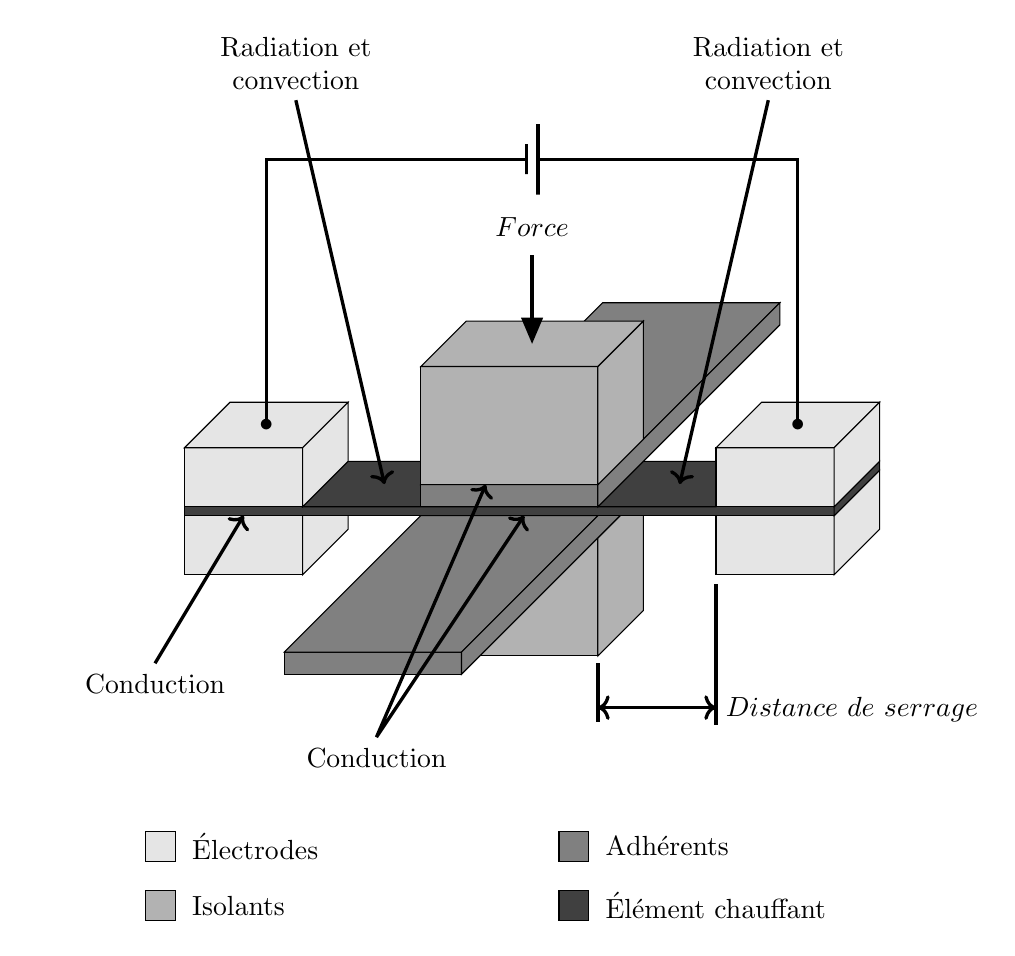
\begin{tikzpicture}[scale=0.75]


%Dimentions du bloc de connection
\def \largconnection{2}
\def \profconnection{2}
\def \hconnection{1.}

%Distance entre les deux blocs
\def \distance_connection{9}

%Épaisseur de l'élément résistif
\def \tele{0.15}

%Distance entre les blocs de connection et l'isolant
\def \gap{2}

%Dimensions des adhérent
\def \lcomp{6}
\def \tcomp{0.375}

%Épaisseur de l'isolant
\def \tbloc{2}

%Position et taille des annotations
\def \hsource{1.25*\profconnection}
\def \hpression{0.75*\profconnection}
\def \legende{0.5}
\def \distcotation{0.125}

%Couleurs
\def \colinsulator{blue!50}
\def \coladherend{green!50}
\def \colconnector{orange!60}
\def \colresistive{gray!50}

\def \colinsulator{black!30}
\def \coladherend{black!50}
\def \colconnector{black!10}
\def \colresistive{black!75}

%Bloc de pression inferieur
\draw[black,fill=\colinsulator] (\largconnection+\gap,-\tcomp-\tele-\tbloc,0) -- ++(0,\tbloc,0) -- ++(\distance_connection-\gap-\gap-\largconnection,0,0) -- ++(0,-\tbloc,0) -- cycle; %Face du devant
\draw[black,fill=\colinsulator] (\distance_connection-\gap,-\tcomp-\tele-\tbloc,0) -- ++(0,\tbloc,0) -- ++(0,0,-\profconnection) -- ++(0,-\tbloc,0) -- cycle; %Face de droite

%Adherant inferieur
\draw[black,fill=\coladherend] (\largconnection+\gap,-\tele-\tcomp,\lcomp) -- ++(0,\tcomp,0) -- ++(\distance_connection-\gap-\gap-\largconnection,0,0) -- ++(0,-\tcomp,0) -- cycle; %Face du devant
\draw[black,fill=\coladherend] (\largconnection+\gap,-\tele,\lcomp) -- ++(0,0,-\lcomp) -- ++(\distance_connection-\gap-\gap-\largconnection,0,0) -- ++(0,0,\lcomp) -- cycle; %Face du dessus
\draw[black,fill=\coladherend] (\distance_connection-\gap,-\tele,\lcomp) -- ++(0,-\tcomp,0) -- ++(0,0,-\lcomp-\profconnection) -- ++(0,\tcomp,0) -- cycle; %Face de droite

%Connection gauche inferieur
\draw[black, fill=\colconnector] (0,-\tele-\hconnection,0)--++(\largconnection,0,0)--++(0,\hconnection,0)--++(-\largconnection,0,0)--cycle; %Face du devant
\draw[black, fill=\colconnector] (\largconnection,-\tele-\hconnection,0)--++(0,\hconnection,0)-- ++(0,0,-\profconnection)--++(0,-\hconnection,0)--cycle; %Face de droite

%Connection droite inferieur
\draw[black, fill=\colconnector] (\distance_connection,-\tele-\hconnection,0)--++(\largconnection,0,0)--++(0,\hconnection,0)--++(-\largconnection,0,0)--cycle; %Face du devant
\draw[black, fill=\colconnector] (\largconnection+\distance_connection,-\tele-\hconnection,0)--++(0,\hconnection,0)--++(0,0,-\profconnection)--++(0,-\hconnection,0)--cycle; %Face de droite

%Element chauffant
\draw[black,fill=\colresistive] (0,0,0) -- (\largconnection+\distance_connection,0,0) -- ++(0,-\tele,0) -- (0,-\tele,0) -- cycle; %Face du devant
\draw[black,fill=\colresistive] (\largconnection,0,0) -- ++(0,0,-\profconnection) -- (\distance_connection,0,-\profconnection) -- (\distance_connection,0,0) -- cycle; %Face du dessus
\draw[black,fill=\colresistive] (\distance_connection+\largconnection,0,0) -- ++(0,0,-\profconnection) -- ++(0,-\tele,0) -- ++(0,0,\profconnection) -- cycle; %Face de droite

%Adherant superieur
\draw[black,fill=\coladherend] (\largconnection+\gap,0,0) -- ++(0,\tcomp,0) -- ++(\distance_connection-\gap-\gap-\largconnection,0,0) -- ++(0,-\tcomp,0) -- cycle; %Face du devant
\draw[black,fill=\coladherend] (\largconnection+\gap,\tcomp,0) -- ++(0,0,-\lcomp-\profconnection) -- ++(\distance_connection-\gap-\gap-\largconnection,0,0) -- ++(0,0,\lcomp+\profconnection) -- cycle; %Face du dessus
\draw[black,fill=\coladherend] (\distance_connection-\gap,\tcomp,0) -- ++(0,-\tcomp,0) -- ++(0,0,-\lcomp-\profconnection) -- ++(0,\tcomp,0) -- cycle; %Face de droite

%Connection gauche superieure
\draw[black, fill=\colconnector] (0,0,0)--(\largconnection,0,0)--++(0,\hconnection,0)--(0,\hconnection,0)--cycle; %Face du devant
\draw[black, fill=\colconnector] (0,\hconnection,0)--++(\largconnection,0,0)--++(0,0,-\profconnection)--++(-\largconnection,0,0)--cycle; %Face du dessus
\draw[black, fill=\colconnector] (\largconnection,0,0)--++(0,\hconnection,0)-- ++(0,0,-\profconnection)--++(0,-\hconnection,0)--cycle; %Face de droite

%Connection droite superieure
\draw[black, fill=\colconnector] (\distance_connection,0,0)--++(\largconnection,0,0)--++(0,\hconnection,0)--++(-\largconnection,0,0)--cycle; %Face du devant
\draw[black, fill=\colconnector] (\distance_connection,\hconnection,0)--++(\largconnection,0,0)--++(0,0,-\profconnection)--++(-\largconnection,0,-0)--cycle; %Face du dessus
\draw[black, fill=\colconnector] (\largconnection+\distance_connection,0,0)--++(0,\hconnection,0)--++(0,0,-\profconnection)--++(0,-\hconnection,0)--cycle; %Face de droite

%Bloc de pression superieur
\draw[black,fill=\colinsulator] (\largconnection+\gap,\tcomp,0) -- ++(0,\tbloc,0) -- ++(\distance_connection-\gap-\gap-\largconnection,0,0) -- ++(0,-\tbloc,0) -- cycle; %Face du devant
\draw[black,fill=\colinsulator] (\largconnection+\gap,\tcomp+\tbloc,0) -- ++(0,0,-\profconnection) -- ++(\distance_connection-\gap-\gap-\largconnection,0,0) -- ++(0,0,\profconnection) -- cycle; %Face du dessus
\draw[black,fill=\colinsulator] (\distance_connection-\gap,\tcomp,0) -- ++(0,\tbloc,0) -- ++(0,0,-\profconnection) -- ++(0,-\tbloc,0) -- cycle; %Face de droite

%Connection de la source de puissance
\draw [very thick] (0.5*\largconnection,\hconnection,-0.5*\profconnection) -- ++(0,\hsource+\tbloc,0) -- ++(0.5*\distance_connection-0.1,0,0) -- ++(0,-0.25,0) -- ++(0,0.5,0);
\draw [very thick] (0.5*\largconnection+\distance_connection,\hconnection,-0.5*\profconnection) -- ++(0,\hsource+\tbloc,0) -- ++ (-0.5*\distance_connection+0.1,0,0) -- ++(0,-0.6,0) -- ++ (0,1.2,0);
\draw (0.5*\largconnection,\hconnection,-0.5*\profconnection) node {$\bullet$} ;
\draw (0.5*\largconnection+\distance_connection,\hconnection,-0.5*\profconnection) node {$\bullet$} ;

%Pression
\draw [very thick, -triangle 45] (0.5*\largconnection+0.5*\distance_connection,\tbloc+\tcomp+\hpression,-0.5*\profconnection) -> ++(0,-\hpression,0);
\draw (0.5*\largconnection+0.5*\distance_connection,\tbloc+\tcomp+\hpression+0.15,-0.5*\profconnection) node[above] {$Force$};

%Clamping distance
\draw [very thick, black] (\distance_connection-\gap,-\tcomp-\tele-\tbloc-\distcotation,0) -- ++(0,-1,0);
\draw [very thick, black] (\distance_connection,-0.5*\tcomp-\hconnection-\distcotation,0) -- ++(0,-1-\tbloc+\hconnection-\tcomp,0);
\draw [very thick, black, <->] ((\distance_connection-\gap,-\tcomp-\tele-\tbloc-\distcotation-0.75,0) -- ++ (\gap,0,0);
\draw (\distance_connection,-0.5*\tcomp-\tcomp-\distcotation-\tbloc-.75,0) node[right] {$Distance \ de \ serrage$};

%Identification des modes de refroidissement
\draw [very thick,<-] (\largconnection+0.5*\gap,0,-0.5*\profconnection) -- ++(-1.5,6.5,0) node[above, text width=3cm, align=center] {{Radiation et \\ convection}};
\draw [very thick,<-]  (\distance_connection-0.5*\gap,0,-0.5*\profconnection) -- ++(1.5,6.5,0) node[above, text width=3cm, align=center] {{Radiation et \\ convection}};
\draw [very thick,<-]  (0.5*\largconnection,-\tele,0) -- ++(-1.5,-2.5,0) node[below, text width=3cm, align=center] {{Conduction}};
\draw [very thick,<->]  (0.5*\distance_connection+0.625*\gap,-\tele,0) -- ++(-2.5,-3.75,0) node[below, text width=3cm, align=center] {{Conduction}} --(0.5*\distance_connection+0.3*\gap,\tcomp,0) ;


%Legende
\begin{scope}[yshift=-11.cm, xshift=-5.5cm]

	\begin{scope}[xshift=-7cm]
		\draw [black, fill=\colconnector] (\distance_connection+1.42*\profconnection,2.5*\tbloc) rectangle ++(\legende,\legende);
		\draw (\distance_connection+1.42*\profconnection+1.25*\legende,2.5*\tbloc+0.5*\legende) node[right]{Électrodes} ;

		\draw [black, fill=\colinsulator] (\distance_connection+1.42*\profconnection,2.5*\tbloc-2*\legende) rectangle ++(\legende,\legende);
		\draw (\distance_connection+1.42*\profconnection+1.25*\legende,2.5*\tbloc-1.5*\legende) node[right]{Isolants} ;
	\end{scope}

	\draw [black, fill=\coladherend] (\distance_connection+1.42*\profconnection,2.5*\tbloc) rectangle ++(\legende,\legende);
	\draw (\distance_connection+1.42*\profconnection+1.25*\legende,2.5*\tbloc+0.5*\legende) node[right]{Adhérents} ;

	\draw [black, fill=\colresistive] (\distance_connection+1.42*\profconnection,2.5*\tbloc-2*\legende) rectangle ++(\legende,\legende);
	\draw (\distance_connection+1.42*\profconnection+1.25*\legende,2.5*\tbloc-1.5*\legende) node[right]{Élément chauffant} ;
\end{scope}
\end{tikzpicture}

	\caption{Schéma du procédé de soudage par résistance avec identification des modes de conduction de chaleur}
	\label{fig:schema_soudage_resistance}
\end{figure}

Lors du soudage par résistance, un élément chauffant poreux est positionné entre les adhérents (Fig.~\ref{fig:schema_soudage_resistance}). 
Généralement, des blocs isolants sont positionnés autour de la soudure pour réduire les pertes thermiques. 
Des électrodes sont fixées aux deux extrémités de l'élément chauffant à une distance variable du bord des adhérents, nommée «distance de serrage». 
Avant d'appliquer un courant dans le système et tout au long du procédé de soudage, une force est appliquée sur la zone à souder. 
Après un temps prédéterminé, la source électrique est arrêtée tout en maintenant la pression sur la soudure pendant le refroidissement. 
Une fois la soudure refroidie en dessous de la température de transition vitreuse des polymères, il est possible de retirer du montage l'assemblage obtenu. 
Il est à noter que l'élément chauffant reste captif de la soudure à la fin du procédé. 
La possibilité de produire des soudures continues en soudage par résistance a également été démontrée en laboratoire \cite{Shi2015a}. 
Les équations de contact intime et d'interdiffusion en situation de soudage non isotherme ont été appliquées par Ageorges \cite{Ageorges1998} et Colak \cite{Colak2002} afin d'approximer théoriquement des fenêtres d'opération. 

Si on fixe la géométrie du montage de soudage et le choix des matériaux, les principaux paramètres ayant une influence sur la qualité du joint sont 
\begin{inparaenum}[(1)]
	\item la puissance électrique, 
	\item le temps de soudage, 
	\item les effets de bords et les modes de conduction de chaleur, et
	\item la pression appliquée sur la soudure. 
\end{inparaenum}
Globalement, il faut également tenir compte des propriétés des matériaux employés ainsi que de la géométrie des composants du montage. 

\begin{figure}[h]
	\centering
	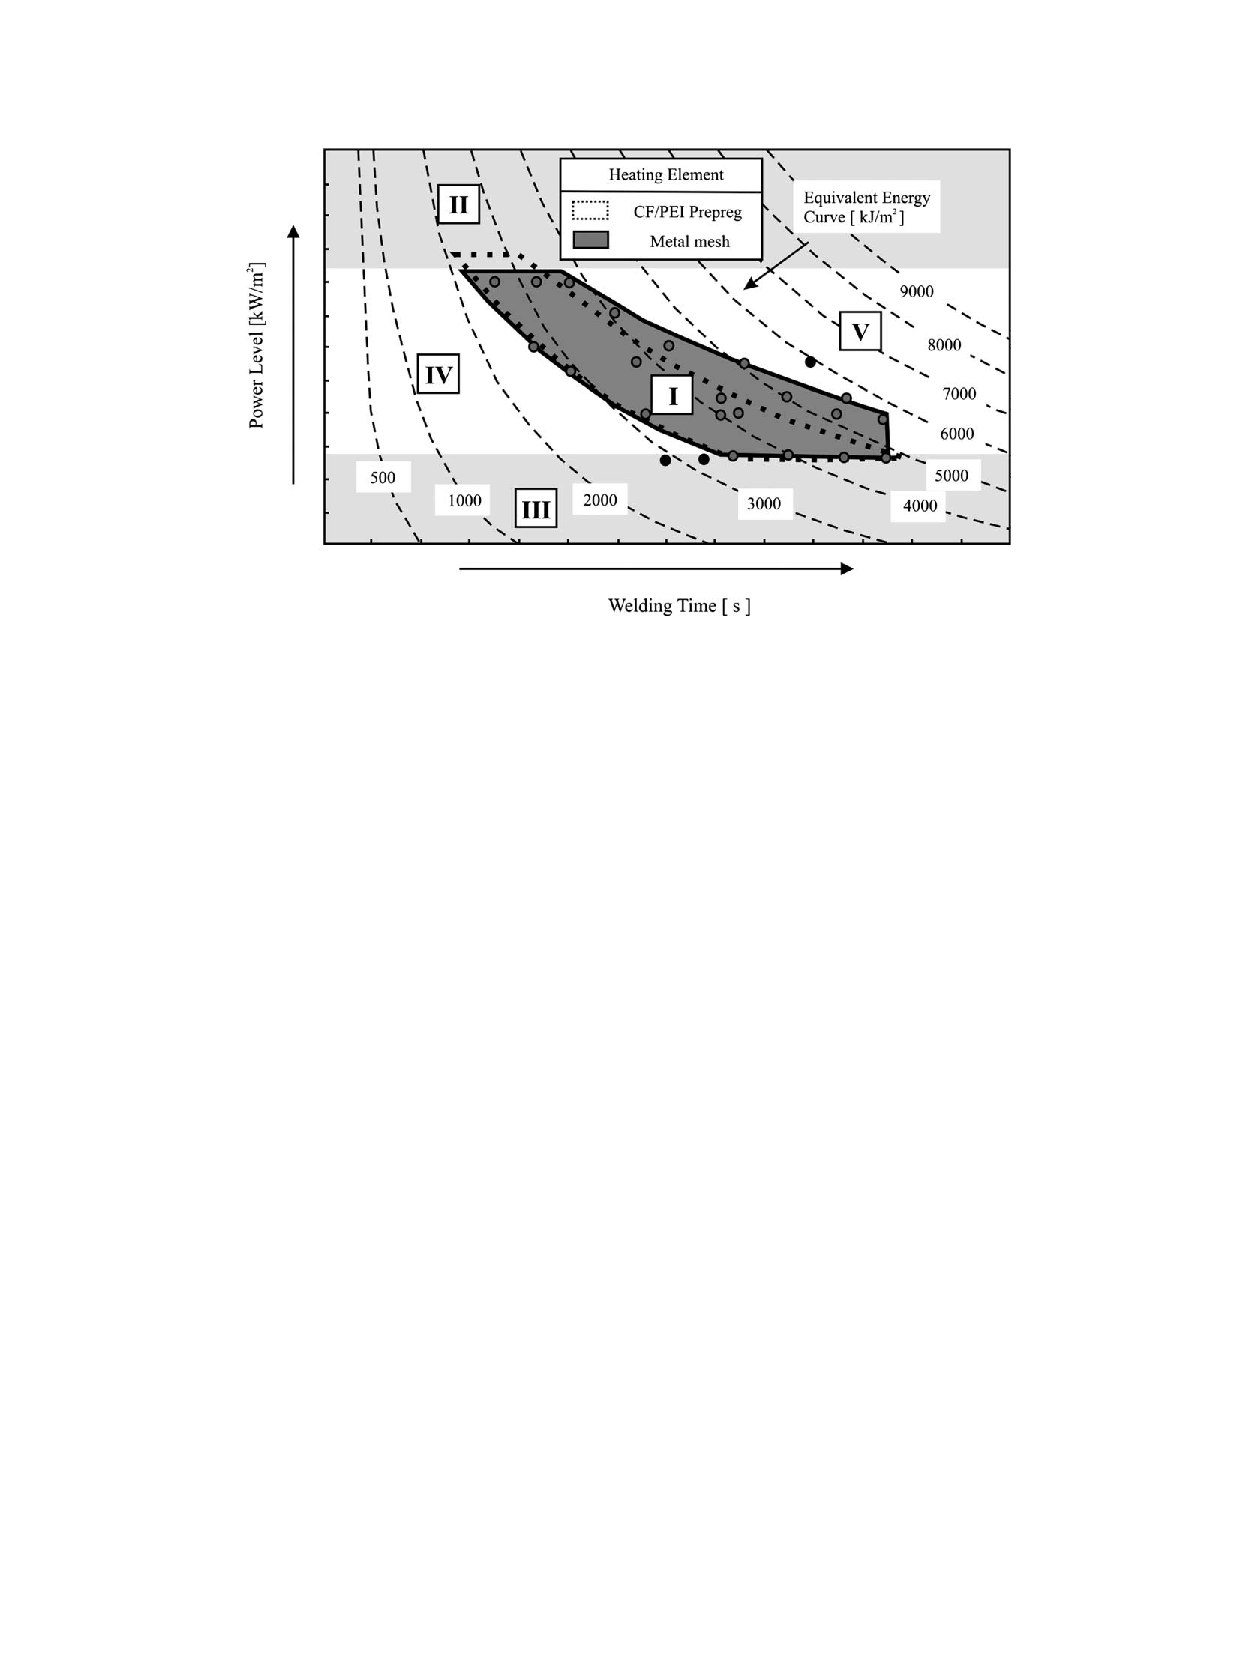
\includegraphics[scale=0.85]{process_window}
	\caption{Fenêtre de puissance pour le procédé de soudage (tirée de \cite{Stavrov2005a}, reproduction avec autorisation)}
	\label{fig:process_window}
\end{figure}

\FloatBarrier
Afin d'optimiser la qualité de la soudure, la puissance électrique et le temps de soudage peuvent facilement être modifiés. 
La plage de puissance ainsi que l'énergie nécessaire (produit de la puissance et du temps) à la production d'une soudure satisfaisante sont documentées dans la littérature \cite{Hou1999a}. 
Lors de l'utilisation de grillages en acier inoxydable comme éléments chauffants, des puissances surfaciques allant de 80 à \SI[locale=FR]{150}{\kilo\watt\per\square\metre} permettent typiquement de produire des soudures satisfaisantes. 
D'autres auteurs (tels que Dubé) ont également utilisé des puissances allant jusqu'à \SI[locale=FR]{282}{\kilo\watt\per\square\metre} avec des temps plus courts \cite{Dube2007}. 
Certains auteurs (tels que Arias) utilisent également de très fortes puissances pulsées de l'ordre de \SI[locale=FR]{600}{\kilo\watt\per\square\metre} avec un temps de repos de quelques secondes entre chaque pulsation afin d'obtenir une température plus uniforme dans la zone soudée et de réduire la quantité d'énergie requise  \cite{Arias1996}. 
Dans presque tous ces cas, les auteurs ont appliqué le courant en maintenant une tension constante ou en produisant une rampe de voltage. 
La résistance des éléments chauffants en acier inoxydable augmente lors de la chauffe entrainant une réduction de la puissance dissipée dans le joint à plus haute température. 
La figure \ref{fig:process_window} présente une fenêtre de puissance de soudage en fonction du temps afin d'obtenir un soudage entre des pièces en composites avec un élément chauffant en acier inoxydable ou en composite de fibre de carbone avec une matrice en PEI. 
Ce graphique présente également des courbes d'énergie équivalente. 
On peut obtenir l'énergie produite en multipliant la puissance au temps d'application selon l'équation : 

\begin{equation}
E = P \times t
\end{equation}

où $E$ est la quantité d'énergie en Joules, $P$ est la puissance en Watts et $t$ est le temps en secondes. 
On peut obtenir la puissance d'un élément chauffant de section constante, en fonction de ses propriétés électriques et de ses dimensions, à l'aide des équations suivantes. Dans ces équations, $V$ est la tension en volts, $I$ est l'intensité du courant en ampères, $R_e$ est la résistance en $\ohm$, $L$ est la longueur en mètres du conducteur, $A_s$ est l'aire de la section du conducteur en mètres carrés et $\rho_{ele}$ est la résistivité en $\ohm \cdot$mètres. 

\begin{equation}
P = V \times I
\end{equation}

\begin{equation}
P = R_e \times I^2
\end{equation}

\begin{equation}
P = \frac{\rho_{ele} \times L}{A_s} \ I^2
\end{equation}

\begin{equation}
P = \frac{V^2}{\rho_{ele}} \ \frac{A_s}{L}
\end{equation}

Il est possible de lier la résistivité ($\rho_{ele}$) d'un matériau à sa conductivité ($\sigma$) en Siemens par mètre à l'aide de l'équation suivante :

\begin{equation}
\sigma = \frac{1}{\rho_{ele}}
\end{equation}

Dans le cas des éléments pour le soudage résistif, ces équations sont simplifiées sous la forme suivante où $l$ est la largeur en mètre du grillage et $\gamma$ est la résistivité spécifique en $\ohm$ :

\begin{equation}
R = \gamma \ \frac{L}{l}
\label{EQ:resistance_element_chauffant}
\end{equation}

Pour utiliser l'équation \ref{EQ:resistance_element_chauffant}, il est nécessaire de caractériser au préalable l'élément chauffant afin de connaitre sa résistance spécifique. 
Cette dernière équation pose également l'hypothèse d'un élément de composition relativement homogène. 
Les effets des dimensions des mailles ainsi que le diamètre des fils ont été étudiés dans la littérature.
Il a été trouvé que le ratio entre le ratio d'aire ouverte et le diamètre du fil est un critère important pour le soudage avec un grillage métallique \cite{Dube2012a}. 

Les effets de bords et les modes de conduction de chaleur dépendent principalement de la géométrie du montage et de la nature des matériaux. 
Cependant, pour un montage de soudage donné, un contrôle limité de ces paramètres est parfois possible en modifiant la distance de serrage des électrodes. 
Comme indiqué à la figure \ref{fig:schema_soudage_resistance}, les pertes thermiques de l'élément chauffant changent de mode de transfert en fonction de leur position dans la soudure. 
Dans les zones où l'élément chauffant est positionné entre les adhérents composites ou lorsqu'il est en contact avec les électrodes, le transfert thermique se produit principalement par conduction. 
Dans les zones où l'élément chauffant est exposé (entre les bords des adhérents et les électrodes), les pertes thermiques se produisent plutôt par radiation et convection naturelle. 
Puisque ces derniers modes de transfert de chaleur sont moins efficaces, un certain contrôle de la température au bord du laminé est possible en ajustant la distance de serrage \cite{Talbot2013}. 
Il est impossible d'éliminer totalement ces effets de bord, mais il est possible de viser des paramètres de soudage qui en réduisent l'impact. 

En ce qui concerne la pression appliquée sur la soudure, plusieurs chercheurs ont présenté l'effet de la pression sur la qualité des soudures obtenues. 
Pour les soudures de laminés avec une matrice en PEI, Ageorges a observé des signes de déconsolidation des laminés lorsqu'une faible pression, de l'ordre de \SI[locale=FR]{0.1}{\mega\pascal}, est employée \cite{Ageorges2000a}.
Il a aussi noté le déplacement des fibres et un trop grand écoulement causé par la compression du laminé lorsqu'une pression supérieure à \SI[locale=FR]{1.6}{\mega\pascal} est employée. 
Il définit une plage de pression entre 0,2 et \SI[locale=FR]{1.6}{\mega\pascal} comme cible. 
Shi a observé quant à lui l'effet de la pression sur la formation de porosités et sur la déconsolidation pour des laminés de fibres de verre et PEI \cite{Shi2017}. 
Les résultats ont démontré qu'une pression d'au moins \SI[locale=FR]{0.8}{\mega\pascal} est nécessaire pour éliminer les porosités à l'interface causées par l'humidité et la déconsolidation du laminé. 

Un phénomène à surveiller lors du soudage résistif est la fuite de courant dans le corps des laminés de fibres de carbone. 
Ce phénomène peut se produire lorsque les bords de l'élément chauffant entrent en contact électrique avec les fibres de carbone du laminé et forment un circuit électrique parallèle à l'élément résistif \cite{Hou1999a,Ageorges2000}. 
Ce nouveau circuit réduit le chauffage de la zone soudée, peut empêcher la soudure au centre du joint et peut dégrader le polymère aux bords \cite{Dube2008}. 
On observe alors des zones chaudes aux bords des laminés et une zone froide au centre (Fig.~\ref{fig:schema_fuite_de_courant}). 
Plusieurs approches existent pour éliminer ce problème. 
Il est possible d'ajouter une couche de fibre de verre isolante entre l'élément chauffant et le laminé \cite{Hou1999a}. 
Cette solution a le désavantage d'ajouter un élément étranger dans la zone soudée et d'augmenter l'épaisseur des joints. 
Il est également possible d'isoler le grillage métallique à l'aide d'un revêtement isolant \cite{Dube2008,Dube2009a}. 
Ce revêtement empêche tout contact électrique entre les fibres et l'élément chauffant. 
Finalement, il est possible d'employer une couche d'un polymère possédant une température de mise en forme inférieure à la température de fonte du polymère de base \cite{Stavrov2005a}. 

\begin{figure}[h]
	\centering
	\usetikzlibrary{arrows,shapes,positioning,shadows,trees,arrows.meta}
\usetikzlibrary{decorations.pathmorphing} % Pour obtenir des lignes de coupes aléatoires
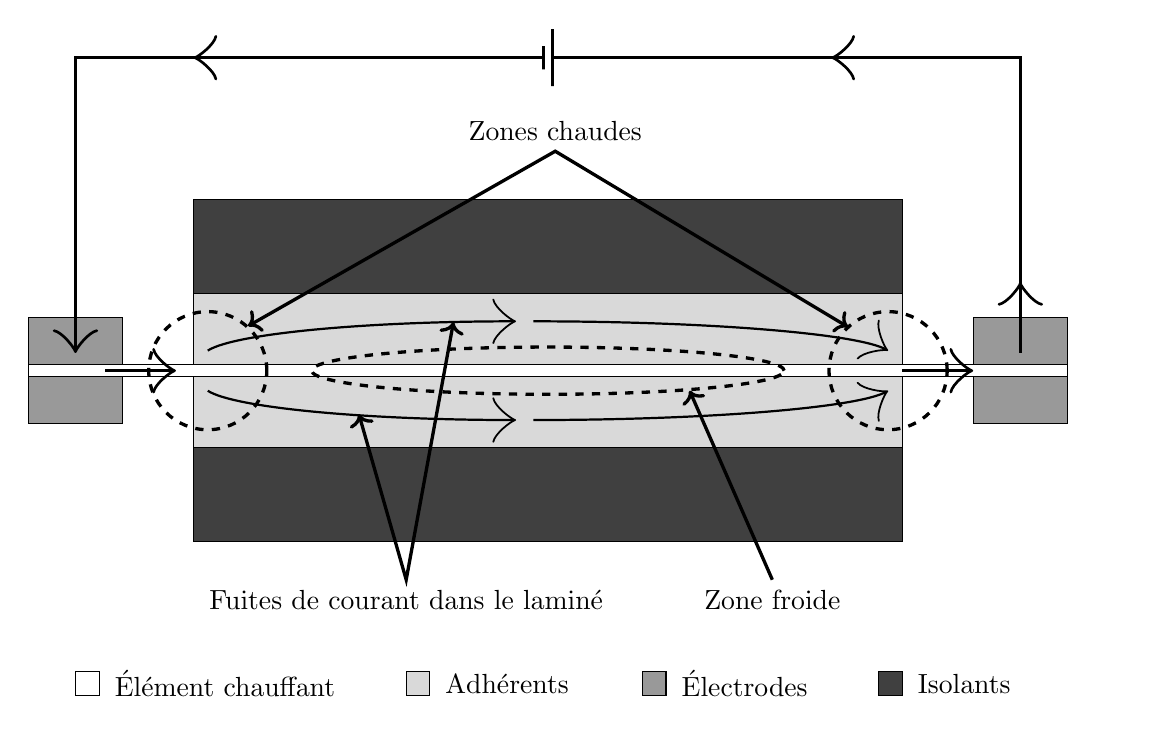
\begin{tikzpicture}[scale=0.6]


%Dimentions du bloc de connection
\def \largconnection{2}
\def \hconnection{1.}

%Distance entre les deux blocs
\def \distance_connection{20}

%Épaisseur de l'élément résistif
\def \tele{0.25}

%Distance entre les blocs de connection et l'isolant
\def \gap{1.5}

%Dimensions des adhérent
\def \tcomp{1.5}

%Épaisseur de l'isolant
\def \tbloc{2}

%Position et taille des annotations
\def \hsource{3.5}
\def \legende{0.5}
\def \distcotation{0.125}

%Couleurs
\def \colinsulator{blue!50}
\def \coladherend{green!50}
\def \colconnector{orange!60}
\def \colresistive{gray!50}

\def \colinsulator{black!75}
\def \coladherend{black!15}
\def \colconnector{black!40}
\def \colresistive{black!0}

%Bloc de pression inferieur
\draw[black,fill=\colinsulator] (\largconnection+\gap,-\tcomp-\tele-\tbloc) -- ++(0,\tbloc) -- ++(\distance_connection-\gap-\gap-\largconnection,0) -- ++(0,-\tbloc) -- cycle; %Face du devant

%Adherant inferieur
\draw[black,fill=\coladherend] (\largconnection+\gap,-\tele-\tcomp) -- ++(0,\tcomp) -- ++(\distance_connection-\gap-\gap-\largconnection,0) -- ++(0,-\tcomp) -- cycle; %Face du devant

%Connection gauche inferieur
\draw[black, fill=\colconnector] (0,-\tele-\hconnection)--++(\largconnection,0)--++(0,\hconnection)--++(-\largconnection,0)--cycle; %Face du devant


%Connection droite inferieur
\draw[black, fill=\colconnector] (\distance_connection,-\tele-\hconnection,0)--++(\largconnection,0,0)--++(0,\hconnection,0)--++(-\largconnection,0,0)--cycle; %Face du devant


%Element chauffant
\draw[black,fill=\colresistive] (0,0,0) -- (\largconnection+\distance_connection,0,0) -- ++(0,-\tele,0) -- (0,-\tele,0) -- cycle; %Face du devant


%Adherant superieur
\draw[black,fill=\coladherend] (\largconnection+\gap,0,0) -- ++(0,\tcomp,0) -- ++(\distance_connection-\gap-\gap-\largconnection,0,0) -- ++(0,-\tcomp,0) -- cycle; %Face du devant


%Connection gauche superieure
\draw[black, fill=\colconnector] (0,0,0)--(\largconnection,0,0)--++(0,\hconnection,0)--(0,\hconnection,0)--cycle; %Face du devant

%Connection droite superieure
\draw[black, fill=\colconnector] (\distance_connection,0,0)--++(\largconnection,0,0)--++(0,\hconnection,0)--++(-\largconnection,0,0)--cycle; %Face du devant

%Bloc de pression superieur
\draw[black,fill=\colinsulator] (\largconnection+\gap,\tcomp,0) -- ++(0,\tbloc,0) -- ++(\distance_connection-\gap-\gap-\largconnection,0,0) -- ++(0,-\tbloc,0) -- cycle; %Face du devant


%Connection de la source de puissance
\draw [very thick] (0.5*\largconnection,\hconnection) -- ++(0,\hsource+\tbloc) -- ++(0.5*\distance_connection-0.1,0) -- ++(0,-0.25) -- ++(0,0.5);
\draw [very thick] (0.5*\largconnection+\distance_connection,\hconnection) -- ++(0,\hsource+\tbloc) -- ++ (-0.5*\distance_connection+0.1,0) -- ++(0,-0.6) -- ++ (0,1.2);


%Courant dans le laminé
\draw[thick, -{Classical TikZ Rightarrow[length=3mm]} ] (\largconnection+1.2*\gap,0.2*\tcomp) arc (170 : 90 : {0.5*\distance_connection-2.25*\gap} and 0.75);
\draw[thick, -{Classical TikZ Rightarrow[length=3mm]} ] (\largconnection+1.2*\gap,-0.2*\tcomp-\tele) arc (-10 : -90 : -{0.5*\distance_connection+2.25*\gap} and 0.75);
\draw [thick, {Classical TikZ Rightarrow[length=3mm]}- ] (\distance_connection-1.2*\gap,0.2*\tcomp) arc (10 : 90 : {0.25*\distance_connection+1.75*\gap} and 0.75);
\draw [thick, {Classical TikZ Rightarrow[length=3mm]}- ] (\distance_connection-1.2*\gap,-0.2*\tcomp-\tele) arc (-10 : -90 : {0.25*\distance_connection+1.75*\gap} and 0.75);
\draw [very thick, {Classical TikZ Rightarrow[length=3mm]}- ] (0.5*\largconnection,0.25*\hconnection) -- ++(0,1.5);
\draw [very thick, -{Classical TikZ Rightarrow[length=3mm]}] (0.5*\largconnection+\distance_connection,0.25*\hconnection) -- ++(0,1.5);
\draw [very thick, -{Classical TikZ Rightarrow[length=3mm]}] (\largconnection-0.25*\gap,-0.5*\tele) -- ++(1*\gap,0);
\draw [very thick, -{Classical TikZ Rightarrow[length=3mm]}] (\distance_connection-1*\gap,-0.5*\tele) -- ++(1.*\gap,0);
\draw [very thick, -{Classical TikZ Rightarrow[length=3mm]}] (\distance_connection-1*\gap,\hconnection+\hsource+\tbloc) -- ++(-\gap,0);
\draw [very thick, -{Classical TikZ Rightarrow[length=3mm]}] (\largconnection+2*\gap,\hconnection+\hsource+\tbloc) -- ++(-1.*\gap,0);

%Identification des fuites de courant
\draw [very thick,<->]  (0.35*\distance_connection,-\tele-0.8) -- ++(1,-3.5) node[below, text width=9cm, align=center] {{Fuites de courant dans le laminé}} --(0.45*\distance_connection,\tcomp-0.6) ;

% zones chaudes
\begin{scope}[radius=1.25, very thick, dashed]
\draw (\largconnection+\gap+0.3,-0.5*\tele) circle ;
\draw (-\gap+\distance_connection-0.3,-0.5*\tele) circle ;
\end{scope}
\draw [very thick,<->]  (\largconnection+\gap+1.155,0.82) -- ++(6.5,3.7) node[above, text width=9cm, align=center] {{Zones chaudes}} --(-\gap+\distance_connection-1.15,\tcomp-0.7) ;

% zone froide
\draw [very thick, dashed] (0.5*\distance_connection+0.5*\largconnection,-0.5*\tele) ellipse [x radius=5,y radius=0.5] ;
\draw [very thick,<-]  (0.7*\distance_connection,-\tele-0.3) -- ++(1.75,-4) node[below, text width=9cm, align=center] {{Zone froide}} ;

%Legende
\begin{scope}[yshift=-12.cm, xshift=1cm]

\begin{scope}[xshift=12cm]
\draw [black, fill=\colconnector] (0,2.5*\tbloc) rectangle ++(\legende,\legende);
\draw (1.25*\legende,2.5*\tbloc+0.5*\legende) node[right]{Électrodes} ;
\end{scope}

\begin{scope}[xshift=7cm]
\draw [black, fill=\coladherend] (0,2.5*\tbloc) rectangle ++(\legende,\legende);
\draw (1.25*\legende,2.5*\tbloc+0.5*\legende) node[right]{Adhérents} ;
\end{scope}

\begin{scope}[xshift=0cm]
\draw [black, fill=\colresistive] (0,2.5*\tbloc) rectangle ++(\legende,\legende);
\draw (1.25*\legende,2.5*\tbloc+0.5*\legende) node[right]{Élément chauffant} ;
\end{scope}

\begin{scope}[xshift=17cm]
\draw [black, fill=\colinsulator] (0,2.5*\tbloc) rectangle ++(\legende,\legende);
\draw (1.25*\legende,2.5*\tbloc+0.5*\legende) node[right]{Isolants} ;
\end{scope}

\end{scope}
\end{tikzpicture}

	\caption{Schéma du phénomène de fuite de courant}
	\label{fig:schema_fuite_de_courant}
\end{figure}

\FloatBarrier
Le soudage par résistance des composites thermoplastiques est généralement réalisé avec un élément chauffant en acier inoxydable ou encore en fibre de carbone. 
Initialement, il était naturel pour les chercheurs d'utiliser un élément chauffant en composite à fibres de carbone \cite{Ageorges2000a,houghton1984bonding,Eveno1988}. 
Cependant, des problèmes persistants étaient causés par la connexion électrique avec les fibres ainsi que par le manque de répétabilité dans les résultats obtenus et la mise à l'échelle \cite{McKnight1997}. 
Le passage à des éléments chauffants en acier inoxydable a permis d'améliorer grandement la répétabilité du procédé ainsi que sa capacité à être mis à l'échelle \cite{Hou1999a}.  
Par contre, dans certaines circonstances, le manque d'adhésion entre les éléments chauffants en acier inoxydable et la matrice peut être le point faible d'une soudure par résistance \cite{Dube2007,Dube2012a,Dube2009a,Shi2014,Shi2015a}. 
Également, les éléments chauffants métalliques pourraient causer une augmentation de l'écho radar \cite{Ageorges2001a}. 

\FloatBarrier
\subsection{Soudage avec matériaux mixtes}

Les composites à matrice thermoplastique peuvent également être joints à d'autres matériaux. 
Plusieurs chercheurs ont développé des méthodes de soudage entre des adhérents thermoplastiques et métalliques. 
Les méthodes employées varient du soudage au point par friction \cite{Goushegir2016}, au soudage par ultrasons \cite{Balle2009,Kruger2004} jusqu'à des combinaisons de soudage par laser avec un chauffage par induction \cite{Weidmann2018}. 
Ce dernier exemple se démarque par une approche où l'adhérent métallique est texturé à l'aide d'un laser. 
Lors du soudage subséquent, le polymère vient remplir les porosités créées en surface pour obtenir un blocage mécanique entre les matériaux. 
Ce procédé a d'ailleurs fait l'objet d'une démonstration technologique visant à présenter une cellule de production automatisée pour des pièces du domaine de l'automobile \cite{Gardiner2019a}. 

En plus des métaux, il est possible dans certains cas de souder des adhérents en composites à matrice thermodurcissable. 
En employant une couche de polymère thermoplastique moulée avec le thermodurcissable lors de sa fabrication, Lionetto \cite{Lionetto2018a} et Fernandez Villegas \cite{FernandezVillegas2015} ont pu souder des composites thermoplastiques avec des pièces en époxy.

\section{Nanocomposites conducteurs}

Les nanocomposites sont définis par l'Office québécois de la langue française depuis 2005 comme : 

\begin{quote}
	\textit{Matériau[x] qui comporte[nt] deux ou plusieurs phases distinctes dont une au moins intègre des éléments qui possèdent une dimension pouvant varier entre 1 et 100 nanomètres.}
\end{quote}

Les nanocomposites sont constitués, au minimum, d'une matrice, souvent polymérique, et de particules de taille nanométrique. 
L'ajout de nanoparticules aux polymères permet entre autres de modifier leurs propriétés mécaniques \cite{Thostenson2002a}, électriques \cite{Zheng2003a}, optiques \cite{Hu2014} et thermiques \cite{Diez-Pascual2009, Al-Saleh2009c}. 
Les nanocomposites se retrouvent notamment dans des applications comme la protection contre la foudre et les interférences électromagnétiques, le dégivrage des surfaces, les capteurs et la cryptographie \cite{Andrews2001, Thostenson2001c, Mittal2014h, Gaztelumendi2017, Chu2014, Hu2016, Al-Saleh2009, Chopra2003}. 

Les modifications des propriétés conférées par les nanoparticules sont dépendantes de leurs propriétés propres ainsi que de leur géométrie. 
Les propriétés exceptionnelles des nanoparticules proviennent en partie du ratio entre leur surface et leur volume. 
Elles exposent des surfaces spécifiques beaucoup plus importantes que tout autre matériau macroscopique. 

En raison de leur excellente conductivité électrique, les nanoparticules à base de carbone sont utilisées dans ce projet. 
Les nanoparticules métalliques telles que les nanofibres d'argent ou de cuivre n'ont pas été retenues au début du projet en raison de leur cout plus élevé et des faibles volumes disponibles commercialement. 
Pour cette raison, les prochaines sections de la revue de l'état des connaissances se concentrent sur les nanoparticules à base de carbone ainsi que sur leurs nanocomposites associés. 

\subsection{Nanotubes de carbone}

Découverts accidentellement en 1991 \cite{iijima1991}, les nanotubes de carbone se retrouvent maintenant dans presque tous les domaines de la science des matériaux et de nouvelles applications leur sont trouvées régulièrement. 
Les nanotubes de carbone sont composés d'une structure régulière de feuilles graphitiques de carbone enroulées et jointes pour former un ou des tubes concentriques qui peuvent être refermés aux extrémités par des structures sphériques (Fig.~\ref{structure_nanotube}). 
Généralement, leur diamètre varie entre 2 et \SI{80}{\nano\metre} en fonction du nombre de couches et ils peuvent présenter des rapports de forme supérieurs à 1000. 

\begin{figure}[htb]
	\centering
	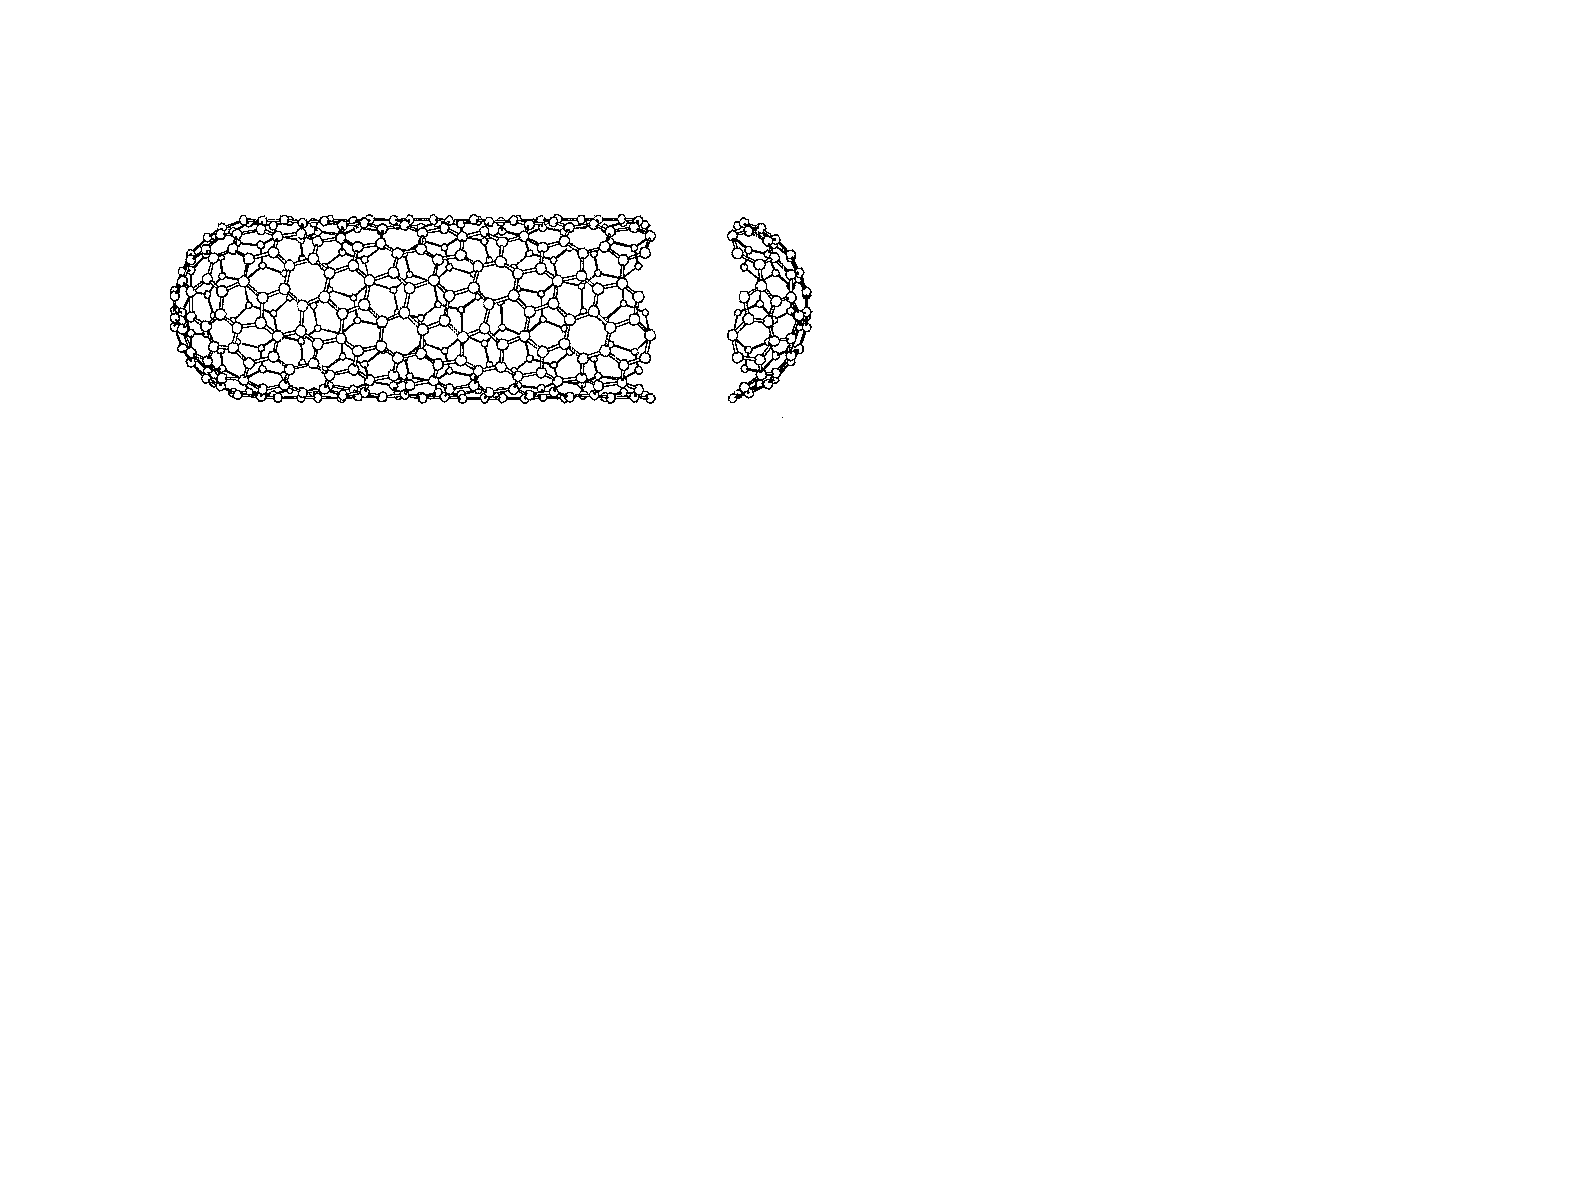
\includegraphics[width=0.5\textwidth]{Saito1992.pdf}
	\caption{Structure d'un nanotube de carbone (adaptée de \cite{Saito1992}, reproduction avec autorisation)}
	\label{structure_nanotube}
\end{figure}

On différencie les nanotubes à simple paroi des nanotubes à parois multiples où plusieurs tubes se forment de façon concentrique. 
Le comportement des nanotubes est fonction de l'angle d'hélice de la structure. 
Pour les nanotubes à simple paroi, on peut obtenir des nanotubes aux propriétés métalliques jusqu'à semi-conductrices avec des variations de cet angle~\cite{Saito1992}. 
Des traitements permettent de purifier les nanotubes et surtout de les séparer selon leur comportement \cite{Makama2013}. 
Généralement, pour les nanotubes multiparois, l'angle d'hélice est moins bien contrôlé et varie d'une couche à l'autre.
On obtient ainsi des nanotubes aux propriétés intermédiaires. 

Les nanotubes de carbone ont des conductivités électriques allant jusqu'à \SI[locale=FR]{10e6}{\siemens\per\centi\metre}  \cite{Sathyanarayana2013} et thermiques de l'ordre de \SI[locale=FR]{6600}{\watt\per\metre\per\kelvin} \cite{Berber2000}. 
Ces propriétés sont fortement dépendantes de l'orientation et de la présence de défauts dans la structure cristalline des nanotubes. 
Les modules de Young rapportés pour les nanotubes de carbone multiparois sont aux alentours de \SI{2}{\tera\pascal} avec des résistances à la traction entre 11 et \SI[locale=FR]{63}{\giga\pascal} \cite{Mittal2014h}. 
Les propriétés des nanotubes de carbone en font d'excellents candidats pour la fabrication de nanocomposites. 

\begin{figure}[htb]
	\centering
	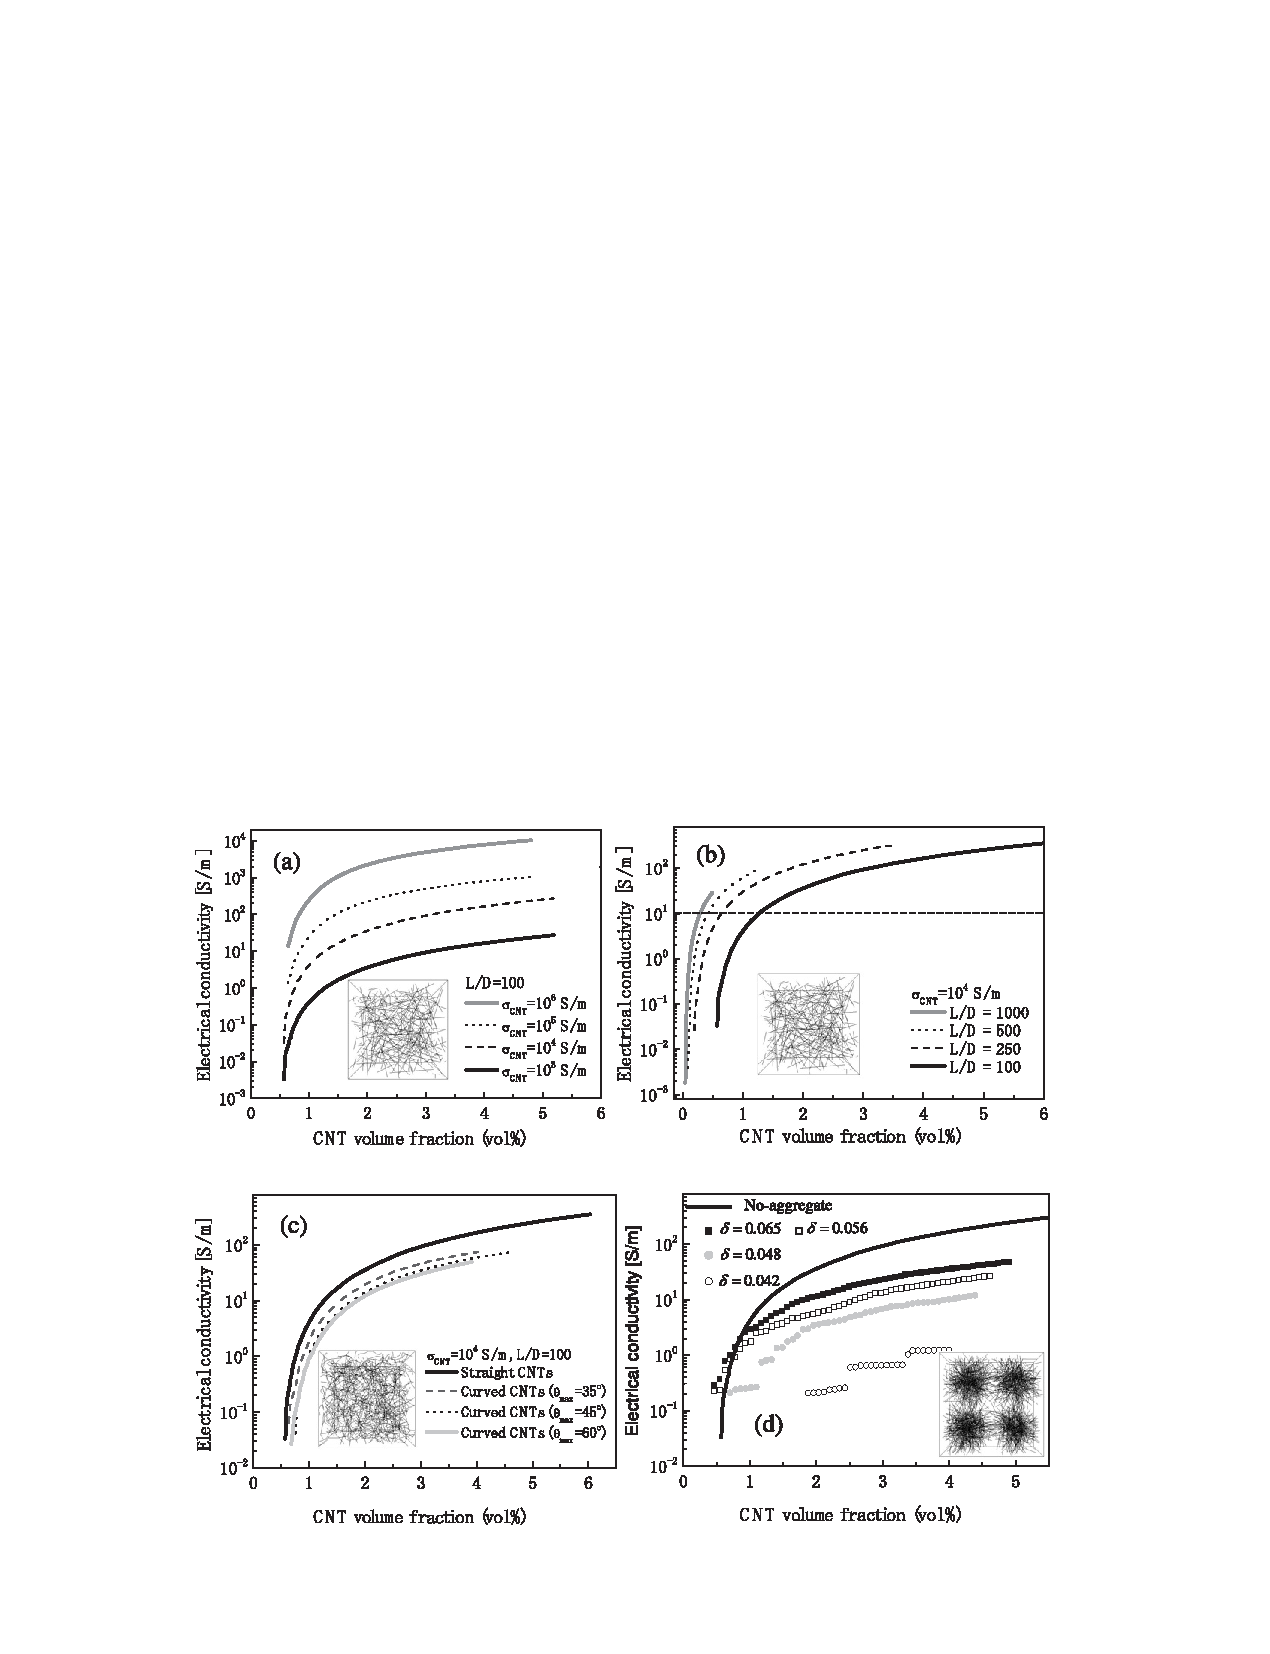
\includegraphics[width=0.8\textwidth]{Hu2008_Fig9.pdf}
	\caption{Effets simulés a) de la conductivité électrique intrinsèque des nanotubes, b) du facteur de forme des nanotubes, c) du niveau de courbure des nanotubes et d) du niveau d'agglomération sur la conductivité électrique des nanocomposites (tirée de \cite{Hu2008}, reproduction avec autorisation)}
	\label{fig:facteurs_geometriques_CNT}
\end{figure}

\FloatBarrier
Les nanotubes de carbone sont principalement produits par décharge d'arc, par ablation laser, par déposition chimique en phase vapeur \cite{Sathyanarayana2013} ou à l'aide de torches au plasma \cite{Kim2009e}. 
Les nanotubes produits peuvent présenter des défauts de cristallinité tels que la présence de pentagones et d'heptagones ou encore des absences dans la structure régulière d'hexagones. 
Ces défauts affectent les propriétés, mais peuvent également être utilisés pour introduire des fonctionnalisations de surface. 

Il est également nécessaire d'ajouter que la conductivité électrique intrinsèque des nanotubes, leur facteur de forme, leur courbure et leur niveau d'agglomération ont tous un impact sur la conductivité électrique des nanocomposites produits (Fig.~\ref{fig:facteurs_geometriques_CNT}). 
Un facteur de forme plus élevé permet d'obtenir une conductivité électrique plus élevée et un seuil de percolation plus bas en raison de la résistance électrique de contact non négligeable entre les nanotubes \cite{Hu2008}. 

\subsection{Nanofibres de carbone}

Les nanofibres de carbone partagent un bon nombre de similarités avec les nanotubes de carbone, mais à un cout beaucoup plus faible. 
Elles sont produites par déposition chimique en phase vapeur tout comme les nanotubes de carbone. 
Elles peuvent ensuite être graphitisées pour améliorer leur pureté et augmenter leur conductivité électrique \cite{Al-Saleh2009c}. 
La principale différence entre les nanotubes et les nanofibres se situe sur le plan de leur morphologie et de leur taille. 
Au lieu d'une structure tubulaire, les nanofibres ont généralement une structure semblable à des bols empilés pour former une série de couches. 
Ces couches superposées peuvent être distinctes ou liées ensemble en spirale \cite{Al-Saleh2009c}. 
Cette structure est différente des tubes circulaires qui composent les nanotubes. 
Également les diamètres des nanofibres sont légèrement plus grands que pour les nanotubes et se trouvent entre 70 et \SI{200}{\nano\metre}. 
Les propriétés des nanofibres sont similaires à celles des nanotubes de carbone, mais avec un niveau de conductivité électrique réduit. 

\subsection{Graphène}

Les nanoparticules de graphène possèdent la même structure hexagonale d'atomes de carbone que les parois des nanotubes de carbone. 
Cependant, au lieu de former un tube, les atomes forment des couches planes de l'épaisseur d'un seul atome de carbone. 
Ces plans atomiques se superposent pour former des plaquettes pouvant ensuite être séparées par exfoliation. 
Le graphène peut également être intégré à un polymère pour en augmenter la conductivité électrique \cite{Jin2013,Wu2012a,Dweiri2015}. 

\subsection{Combinaison de charges}

Certains auteurs ont tenté de démontrer la présence d'une synergie lorsque des charges de différents facteurs de forme ou de différentes tailles sont employées \cite{Kumar2010,Huang2012a,Dweiri2015,Wei2010,Safdari2012}.
Selon les travaux de Kumar, avec une proportion constante de 0,5\% de charges conductrices, la combinaison de nanoplaquettes de graphène et de nanotubes de carbone a obtenu une conductivité électrique supérieure à un nanocomposite composé uniquement de nanoplaquettes de graphène et légèrement supérieure à un nanocomposite avec uniquement des nanotubes de carbone \cite{Kumar2010}. 
Kumar attribue ces résultats au fait que les nanoplaquettes de graphène agiraient comme une protection des nanotubes durant la mise en forme par ultrasonification en leur permettant de conserver leur facteur de forme et ainsi leur contribution à l'augmentation de la conductivité du nanocomposite. 
Dans ses travaux sur des nanocomposites à matrice d'époxy avec de grandes concentrations de charges, Huang dénote quant à lui l'absence de synergie lorsque le taux de renfort est supérieur à 30\% \cite{Huang2012a}. 
Cependant, d'autres chercheurs présentent des résultats beaucoup plus mitigés \cite{Dweiri2015,Wei2010}. 
Ces derniers dénotent une augmentation de la conductivité lorsqu'une partie des charges de graphène ou de noir de carbone sont remplacées par des nanotubes de carbone. 
Cet effet peut être expliqué simplement par le facteur de forme des nanotubes de carbone qui est beaucoup plus avantageux pour obtenir un réseau percolé \cite{Safdari2012}. 
Ainsi, la combinaison de charges conductrices peut parfois être bénéfique, mais il n'existe pas de consensus scientifique quant à la méthode pour généraliser ces résultats. 

\subsection{Méthodes de production des nanocomposites}

Pour tirer profit à l'échelle macroscopique des propriétés des nanomatériaux, il est nécessaire de les mélanger dans une matrice. 
Plusieurs méthodes permettent d'obtenir des mélanges avec les polymères thermoplastiques (Tab. \ref{tab:methodes_de_melange}). 

Une première méthode est la dispersion des nanotubes dans un solvant \cite{Mohammad2006}.
Lors de cette procédure, les nanotubes sont mis en suspension métastable dans un solvant. 
Par la suite, des surfactants sont souvent utilisés pour stabiliser les dispersions de nanoparticules \cite{Huang2012}. 
Cette méthode est appropriée pour les polymères solubles, les polymères à très faible viscosité et pour les monomères \cite{Ma2010}. 
Pour obtenir une distribution homogène, il est nécessaire d'employer un générateur d'ultrasons afin de séparer les agglomérats de nanoparticules. 
On peut évaluer la contrainte en cisaillement ($\sigma_s$) à laquelle sont soumis les agglomérats à l'aide de l'équation suivante tenant compte de la viscosité ($\eta$) et de la vitesse de déformation ($\dot{\gamma}$) : 

\begin{equation}
\sigma_s = \eta \dot{\gamma}
\end{equation}

Le brassage dans un bassin à ultrasons ou à l'aide d'une sonde à ultrasons est une des seules méthodes procurant les contraintes nécessaires pour réduire les agglomérats de nanotubes à simple paroi dans des solvants à faible viscosité (contrainte de \SI[locale=FR]{100}{\mega\pascal}), mais elle peut également induire des dommages et raccourcir les tubes \cite{Huang2012}. 
Cette méthode ne doit donc pas être employée sans considération des propriétés nécessaires pour l'application finale, puisque la réduction de la longueur des tubes et les traitements de surface peuvent affecter les propriétés finales \cite{Grossiord2008a, Diez-Pascual2010, Ma2008}.  
Il est à noter que les contraintes nécessaires pour séparer des nanotubes multiparois sont beaucoup plus faibles et que d'autres méthodes peuvent les séparer sans induire autant de dommage à leur structure \cite{Huang2012, Ma2010}. 
Un nanotube simple paroi nécessite une contrainte approximative de \SI[locale=FR]{100}{\mega\pascal} tandis qu'un nanotube multiparois requiert approximativement \SI[locale=FR]{16}{\kilo\pascal} \cite{Huang2012}. 
Le mélange produit par la mise en suspension peut être employé directement si le solvant est par exemple le monomère d'un polymère thermodurcissable ou, si le solvant utilisé peut dissoudre le polymère désiré, il est possible d'obtenir un composite homogène en évaporant le solvant pour conserver les nanoparticules ainsi que le polymère. 

Une seconde méthode de production est le mélange à l'état fondu \cite{Ma2010}. 
Cette méthode est particulièrement applicable aux polymères thermoplastiques.
La viscosité résiduelle du polymère induit des efforts de cisaillement avec des contraintes suffisantes pour réduire les agglomérats de nanotubes multiparois (contraintes en cisaillement de \SI[locale=FR]{20}{\kilo\pascal}) \cite{Huang2012}. 
Ce brassage peut s'effectuer avec un mélangeur mécanique ou à l'aide d'une d'extrudeuse. 
Ces deux dernières techniques de brassage ont l'avantage de ne pas causer de dommages aux nanotubes \cite{Ma2010}. 
De plus, la production de nanocomposites par extrusion offre l'avantage de pouvoir atteindre des taux de renfort très élevés \cite{Ma2010}. 

Une autre technique pouvant s'appliquer aux polymères thermoplastiques est le broyage par boulets. 
Ce processus utilise les chocs et le brassage des billes métalliques dans un contenant fermé en rotation, et ce, dans le but de réduire en poudre les polymères ainsi que les agglomérats de nanotubes.
Cette technique endommage les nanotubes, mais il est possible d'y introduire des composés chimiques pour fonctionnaliser les nanotubes afin de modifier leurs propriétés: par exemple, l'ajout de bicarbonate d'ammonium permet l'obtention de groupes fonctionnels amides et amines améliorant la conductivité électrique des nanotubes \cite{Ma2010, Ma2008a}. 

Les solutions mentionnées précédemment visent à produire des nanocomposites à dispersion homogène dans l'ensemble de la structure. 
Il est également possible de produire des nanocomposites nanostructurés avec une ségrégation des nanocharges qui permet la création d'un réseau continu à une plus petite quantité de nanoparticules \cite{Al-Saleh2011, Li2015a, Deng2014a, Du2011a, Pang2014c, Jia2015}. 
Cette technique permet d'offrir des composites avec une conductivité électrique beaucoup plus élevée. 
Lors de la fusion de ces polymères, il est cependant possible qu'une diffusion des nanocharges se produise et affecte drastiquement les propriétés électriques après le changement dans la nanostructure \cite{Wu2012}. 
Ce comportement pourrait d'ailleurs être utilisé comme méthode pour contrôler la puissance dégagée lors du soudage. 

Un des défis lors de la production des nanocomposites est de stabiliser la séparation des nanoparticules qui ont tendance à s’agglomérer.
Cette stabilité peut être atteinte en augmentant l'affinité des nanoparticules avec la matrice d'accueil ou par répulsion entre elles. 
Ces effets peuvent être obtenus par une fonctionnalisation de la surface des nanotubes \cite{Xie2005}. 
La fonctionnalisation peut affecter les propriétés macroscopiques des nanocomposites \cite{Ma2008}. 

\begin{table}[h]
	\centering
	\caption{Résumé des méthodes de mélange (adapté de \cite{Ma2010})}
	\resizebox{\textwidth}{!}{%
		\begin{tabular}{@{}l p{1.2in} p{2.5in} p{2.75in} @{}}
			\toprule
			Techniques            & Facteurs                    &                                                                                        &                                                                                                     \\
			\cmidrule(l){2-4}     & Endommagement des nanotubes & Types de matrice compatibles                                                           & Principaux paramètres                                                                               \\ \midrule
			Ultrasonification     & Oui                         & Polymère soluble, polymère ou oligomère à faible viscosité, monomère                   & Puissance et mode d'ultrasonification, durée                                                        \\
			Broyage par boulets   & Oui                         & Granules et poudre (polymère ou monomère)                                              & Durée du broyage, vitesse de rotation, taille des boulets, ratio entre les boulets et les nanotubes \\
			Extrusion             & Non                         & Thermoplastiques                                                                       & Température, géométrie et vitesse de rotation de la vis                                             \\
			Mélange par agitation & Non                         & Thermoplastiques, polymère soluble, polymère ou oligomère à faible viscosité, monomère & Taille et géométrie de l'agitateur, vitesse de rotation, temps de mélange                           \\ \bottomrule
		\end{tabular}
	}
	\label{tab:methodes_de_melange}
\end{table}

\FloatBarrier

\subsection{Conductivité électrique des nanocomposites}

L'ajout de nanoparticules conductrices permet de transformer des polymères non conducteurs en nanocomposites conduisant l'électricité. 
Les principaux paramètres qui affectent la conductivité électrique des nanocomposites sont: la quantité de nanoparticules dispersées, leur nature, la qualité de la dispersion, la nature du polymère et les modifications de surface apportées aux nanoparticules. 

Les variations de la conductivité électrique observées ne peuvent pas être expliquées par la simple loi des mélanges. 
À partir d'une certaine concentration, les nanotubes de carbone forment un réseau continu dans la matrice. 
Cette concentration est nommée seuil de percolation.
En dessous du seuil de percolation, la conductivité du nanocomposite reste à peu près stable et ce dernier demeure isolant \cite{Bangarusampath2009}. 
Lorsque le réseau est initialement formé, la conductivité électrique du nanocomposite change totalement et une augmentation très rapide de la conductivité électrique, de l'ordre de plusieurs décades, peut être observée. 
Par la suite, la conductivité du nanocomposite continue d'augmenter avec l'ajout de nanoparticules, mais avec une pente beaucoup plus faible. 
L'évolution de la conductivité électrique d'un nanocomposite suit trois régimes distincts qui sont fonction de la concentration en nanocharges conductrices. 
La figure \ref{fig:percolation_electrique} présente une courbe de conductivité électrique en fonction de la concentration en nanotubes de carbone multiparois dans une matrice de PEEK. 
Le facteur de forme \cite{Hu2008}, le niveau de dispersion, l'orientation des particules dans la matrice \cite{Xie2011c} et les traitements de surface sont des facteurs qui ont un impact direct sur le seuil de percolation. 

\begin{figure}[h]
	\centering
	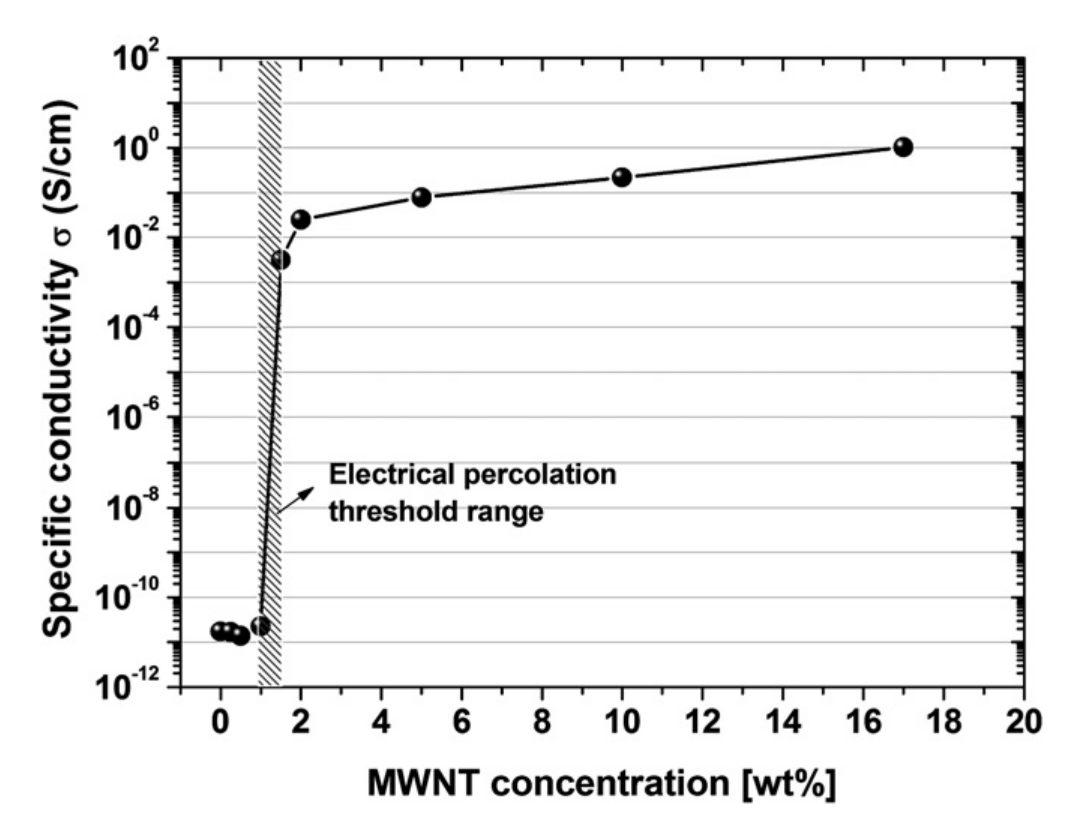
\includegraphics[width=0.7\textwidth]{percolation_electrique.png}
	\caption{Conductivité électrique d'un nanocomposite de PEEK et de nanotubes de carbone (tirée de \cite{Bangarusampath2009}, reproduction avec autorisation)}
	\label{fig:percolation_electrique}
\end{figure}

\FloatBarrier
La plupart des auteurs se concentrent sur la caractérisation du seuil de percolation.
Peu de mesures de conductivité sont donc disponibles pour des concentrations élevées de nanotubes. 
Les plus grands gains en conductivité électrique peuvent être observés à des concentrations s'approchant du seuil de percolation.
La réduction de la concentration en nanotubes permet d'ailleurs de réduire les couts du matériau. 
Les auteurs rapportent des seuils de percolation variant entre 0,0021\% à 15\% \cite{Bauhofer2009}. 
Une portion des résultats publiés sont résumés à la figure \ref{fig:percolation_articles}. 

\begin{figure}[h]
	\centering
	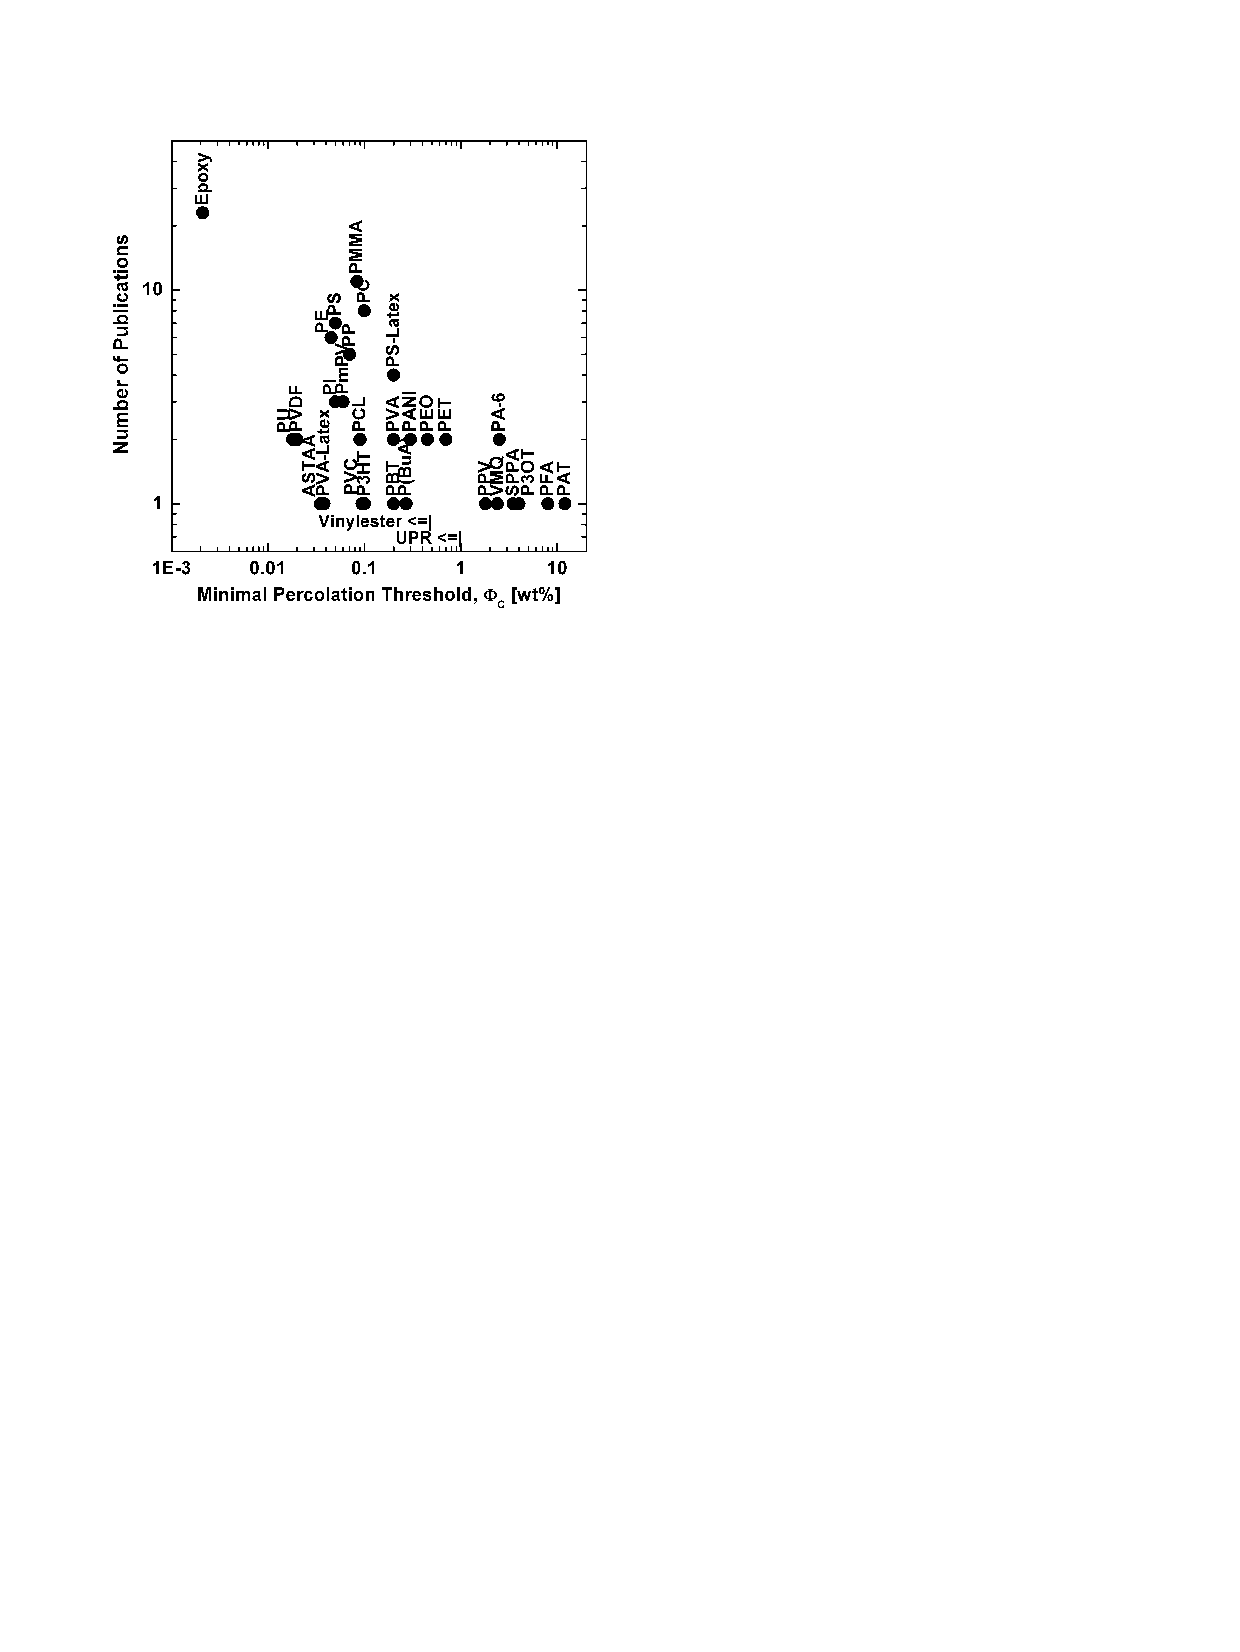
\includegraphics[scale=0.8]{percolation_litterature.pdf}
	\caption{Seuil de percolation minimal reporté et nombre d'articles publiés pour certains systèmes nanocomposites (tirée de \cite{Bauhofer2009}, reproduction avec autorisation)}
	\label{fig:percolation_articles}
\end{figure}

\FloatBarrier
Quant à l'exploration des concentrations plus élevées de nanoparticules conductrices, quelques recherches peuvent être soulignées. 
Par exemple, une conductivité de \SI[locale=FR]{10e4}{\siemens\per\metre} a été atteinte avec une matrice de polyméthacrylate de méthyle (PMMA) et une concentration de 10\% de nanotubes à simple paroi \cite{Bauhofer2009}. 
Pour fins de comparaison, la conductivité électrique de l'acier inoxydable est de \SI[locale=FR]{14.5e5}{\siemens\per\metre}, soit une valeur 15 fois plus élevée. 
Malgré quelques rares résultats exceptionnels, l'ensemble des données publiées présente une très grande variabilité, car un grand nombre de facteurs varient entre chaque étude.
Il n'existe aucune courbe maitresse permettant de généraliser tous ces résultats. 
Le consensus est qu'une bonne dispersion favorise la conductivité électrique \cite{Bauhofer2009} et que les principaux paramètres gouvernant la conductivité sont: le facteur de forme des nanotubes, une bonne dispersion des agglomérats de nanotubes à l'échelle nanométrique et une distribution uniforme des nanotubes ou des agglomérats à l'échelle microscopique \cite{Li2007a}.
Une autre approche pour atteindre le seuil de percolation avec un minimum de charges réside dans la méthode employée pour établir le réseau percolé. 
Celui-ci peut s'obtenir de plusieurs façons. 
Il est possible de disperser les nanotubes de façon à obtenir une mauvaise distribution pour maintenir des contacts entre les agrégats \cite{Al-Saleh2009c,Deng2014a}. 
Cette technique vise à produire une structure similaire à ce qui est présenté à la figure \ref{fig:dispersion_distribution}. 
Autrement, on peut obtenir un réseau percolé aux frontières à l'aide de granules recouvertes de particules conductrices afin d'obtenir une structure ségrégée \cite{Al-Saleh2011,Pang2014c}. 
Finalement, il est possible d'employer l'affinité des nanoparticules afin de les disperser préférentiellement dans une seule phase ou à l'interface d'un mélange binaire de polymères \cite{Pang2014c,Deng2014a}. 

\begin{figure}[h]
	\centering
	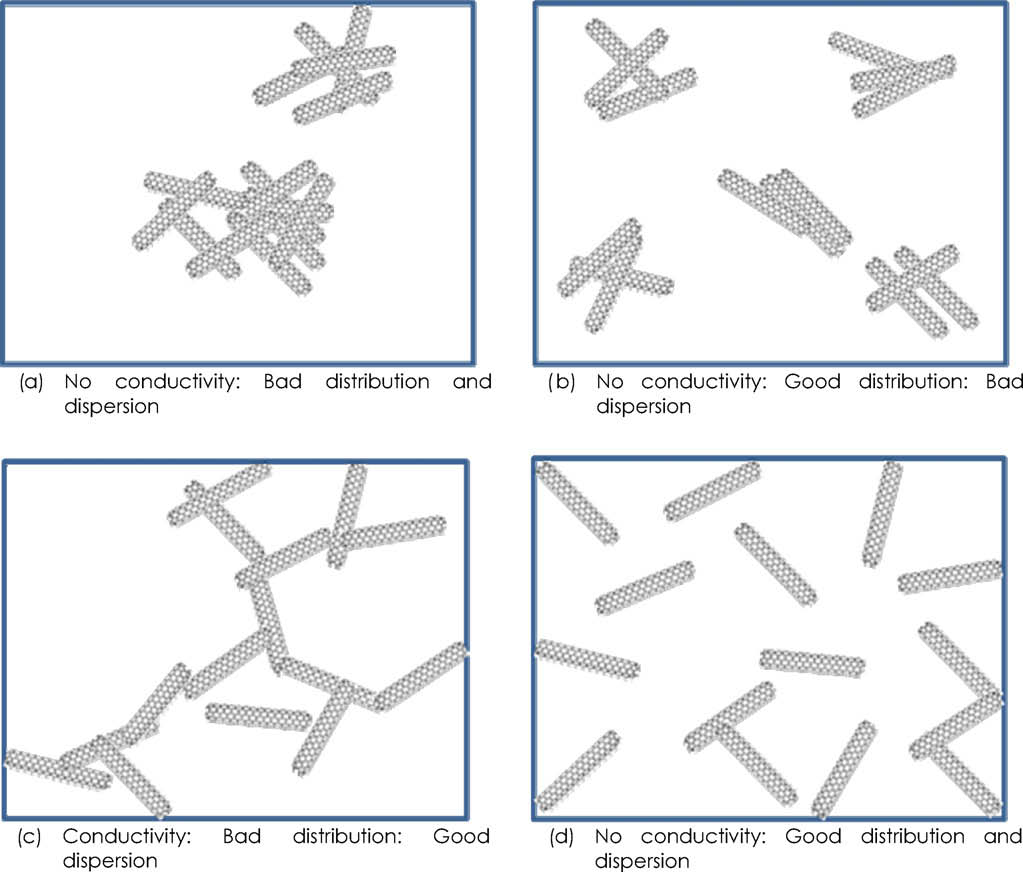
\includegraphics[width=0.6\textwidth]{dispersion_distribution-Al-Saleh2009c.png}
	\caption{Comparaison entre les effets de la distribution et de la dispersion (tirée de \cite{Al-Saleh2009c}, reproduction avec autorisation)}
	\label{fig:dispersion_distribution}
\end{figure}

Également, une fois le seuil de percolation franchi, les conductivités obtenues augmentent moins rapidement que pourrait le suggérer la loi des mélanges. 
Certains travaux \cite{Untereker2009,Cauchy2018} en sont venus à la conclusion que la conductivité électrique obtenue lors du mélange d'une matrice chargée en micro ou nanomatériaux est limitée par la résistance de contact élevée entre les particules. 
La dépendance envers la résistance de contact a également été rapportée par Li \cite{Li2007a}. 

La fonctionnalisation des nanotubes est généralement employée pour faciliter leur dispersion, mais elle peut également affecter les propriétés électriques du nanocomposite. 
Certaines modifications vont entrainer une chute de la conductivité électrique tandis que d'autres vont permettre de réduire la résistance de contact. 

\FloatBarrier
Cette variation des effets selon les divers types de fonctionnalisation par rapport à la conductivité électrique est documentée dans la littérature scientifique. 
Par exemple, il a été démontré que la fonctionnalisation avec des groupes carboxyliques (COOH) produit une réduction très importante de la conductivité \cite{Guadagno2011}. 
Dans cette dernière étude, même en quadruplant la quantité de nanotubes de carbone, les nanotubes fonctionnalisés présentaient une conductivité électrique encore inférieure aux nanotubes non traités. 
La fonctionnalisation avec des groupements amines (NH$_2$) produit également une réduction de la conductivité électrique \cite{Ma2008}.
Il est postulé que cette réduction est en partie due à la dégradation de la structure des nanotubes nécessaire au dépôt des groupes fonctionnels, dégradation qui réduit la conductivité des nanotubes sans réduire la résistance de contact \cite{Pandey2012a}. 
Même dans le cas de particules métalliques, l'ajout d'une fonctionnalisation à base du composé organique 
1-octanethiol cause une baisse de la conductivité électrique \cite{Gelves2008a}. 
Au contraire, le dépôt de particules d'argent a pour effet de permettre une réduction de la résistance de contact et ainsi d'augmenter la conductivité électrique \cite{Ma2010,Cauchy2017}. 

Les méthodes de fonctionnalisation par enroulement de polymères produisent généralement une réduction de la conductivité électrique \cite{Diez-Pascual2010, Huang2012}. 
Vankayala a cependant obtenu une hausse de la conductivité en utilisant du polyaniline (PANI), un polymère conducteur, comme agent de revêtement des nanotubes \cite{Vankayala2011}. 
En utilisant un polymère conducteur compatible avec les nanotubes de carbone et avec une matrice de polycaprolactame, l'auteur a pu réduire la résistance de contact tout en améliorant la dispersion des charges. 

Les considérations quant à l'emploi d'un nanocomposite dans le cadre d'un procédé entrainant la fonte de la matrice polymère ne sont pas explorées dans la littérature. 
L'évolution et le maintien de la conductivité lors de la fonte sont des éléments encore inconnus. 
Dans le cas d'un réseau percolé par ségrégation de phases, la diffusion des particules conductrices lors de la fusion pourrait modifier grandement la conductivité électrique du nanocomposite. 

\subsection{Élément chauffant en assemblage de nanoparticules}

Une autre façon d'employer les nanoparticules conductrices pour obtenir un élément chauffant est l'emploi d'un \textit{buckypaper} ou d'un film de nanotubes alignés. 

Le \textit{buckypaper} peut être composé de plusieurs sortes de nanoparticules dont, entre autres, des nanotubes de carbone ou des nanofibres d'argent. 
Tout comme pour les nanocomposites, un \textit{buckypaper} peut agir comme élément chauffant. 
D'ailleurs, plusieurs chercheurs ont déjà utilisé ce type de solution pour produire des éléments chauffants pouvant servir à dégivrer des surfaces \cite{Pyo2016,Chu2014,Zhang2013}.
Ces chercheurs ont utilisé autant des \textit{buckypaper} de nanotubes de carbone que des feuilles de nanofibres d'argent combinées à un polymère conducteur. 

Pour les films de nanotubes alignés, un film peut être obtenu en enroulant des nanotubes sur un mandrin ou un cadre depuis un substrat sur lequel une forêt de nanotubes a été produite par déposition chimique en phase vapeur. 
Yao a démontré la possibilité d'utiliser un tel film comme système de dégivrage léger pouvant être intégré dans une aile d'avion \cite{Yao2018}.
L'équipe de Russello vient quant à elle de publier un article dans lequel un film de nanotubes alignés est utilisé pour souder par résistance des échantillons de PEEK \cite{Russello2019}. 
Dans ces travaux, un film de nanotubes positionné entre deux films de PEEK était placé entre les deux extrémités de barreaux de PEEK. 
Une résistance en traction égale à 96\% de celle d'un barreau sans soudure a été obtenue. 

\FloatBarrier
\section{Élastomères thermoplastiques}  

% Définition d'une fonction pour dessiner des structures de polymères
\newcommand\setpolymerdelim[2]{\def\delimleft{#1}\def\delimright{#2}}
\def\makebraces[#1,#2]#3#4#5{%
	\edef\delimhalfdim{\the\dimexpr(#1+#2)/2}%
	\edef\delimvshift{\the\dimexpr(#1-#2)/2}%
	\chemmove{%
		\node[at=(#4),yshift=(\delimvshift)]
		{$\left\delimleft\vrule height\delimhalfdim depth\delimhalfdim
			width0pt\right.$};%
		\node[at=(#5),yshift=(\delimvshift)]
		{$\left.\vrule height\delimhalfdim depth\delimhalfdim
			width0pt\right\delimright_{\rlap{$\scriptstyle#3$}}$};}}
\setpolymerdelim()

Un second concept clé pour la réalisation d'une jonction flexible est en lien avec la nature des élastomères thermoplastiques. 
Les élastomères en général sont une famille de polymères dont la plage de température d'utilisation se situe au-dessus de la température de transition vitreuse. 
Au-delà de celle-ci, les polymères entrent en phase caoutchoutique et les chaines peuvent commencer à se déplacer et à glisser les unes par rapport aux autres. 

\begin{figure}[h]
	\centering
	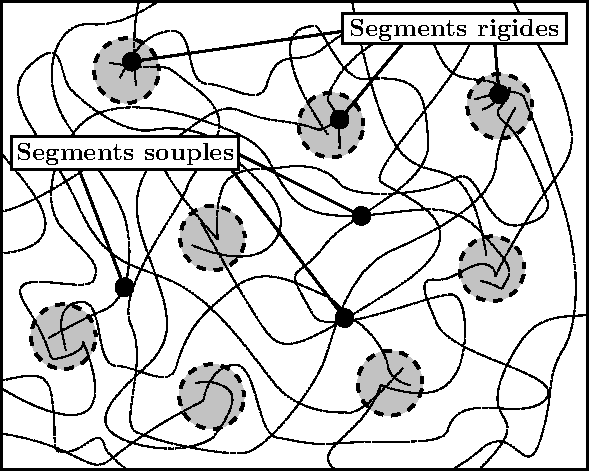
\includegraphics[scale=1]{structure_tribloc.pdf}
	\caption{Exemple de structure pour un élastomère thermoplastique triblocs}
	\label{fig:structure_tribloc}
\end{figure}

Les élastomères commerciaux sont souvent obtenus par une réticulation partielle entre les chaines de polymères, appelée vulcanisation dans le cas de la transformation du  caoutchouc naturel, ayant pour but de bloquer une partie de la mobilité des chaines sans pour autant leur retirer leur flexibilité. 
Les élastomères thermoplastiques obtiennent quant à eux ce comportement à l'aide de leur structure et de leur composition. 
Par l'emploi de segments de natures différentes, on obtient dans les élastomères thermoplastiques triblocs une structure où les terminaisons composées de segments rigides viennent se lier pour former des blocs à l'intérieur de la structure du matériau \cite{Holden1969}. 
En raison de la faible miscibilité entre les deux polymères causée par une incompatibilité thermodynamique, on observe une ségrégation entre les différentes phases (Fig.~\ref{fig:structure_tribloc}) \cite{Scott1952c}. 
Les blocs rigides, composés de polymères qui sont utilisés sous leur température de transition vitreuse, procurent le même effet que la réticulation entre les chaines composées, dans leur portion centrale, d'un second polymère utilisé au-dessus de sa température de transition vitreuse \cite{Holden2002}. 
Les blocs rigides sont également capables de fondre une fois chauffés.
On peut ainsi remettre en forme l'élastomère. 

Les élastomères thermoplastiques ont généralement des structures copolymères en triblocs (Fig \ref{fig:polymere_tri_bloc}) ou multiblocs (Fig.~\ref{fig:polymere_multi_bloc}). 
Les élastomères copolymères triblocs ont des segments rigides aux deux extrémités. 
Ces dernières sont connectées au travers d'un réseau biphasique dans la structure de l'élastomère (Fig.~\ref{fig:structure_tribloc}). 
Contrairement aux élastomères triblocs, figés aux deux extrémités, les élastomères multiblocs utilisent l'enchevêtrement et l'interaction entre les chaines souples et rigides pour maintenir leur intégrité. 
La présence de segments de polymères semi-cristallins au travers d'une chaine amorphe permet aux segments cristallins de se lier pour bloquer l'écoulement de la structure (Fig.~\ref{fig:structure_TPECryst}). 
Alternativement, dans certains cas, les segments cristallins peuvent également être des segments de polymères amorphes \cite{Holden2002}. 

\vspace{6pt}
\begin{figure}[h]
	\subfigcapskip=6pt
	\centering
	\subfigure[][]
	{\label{fig:polymere_alternee} 								
		\chemfig{\vphantom{B}-[@{op,.75}]A-B-[@{cl,0.25}]}
		\makebraces[5pt,5pt]{\!\!n}{op}{cl}
		\bigskip
	} \quad
	\subfigure[]
	{\label{fig:polymere_tri_bloc} 					
		\chemfig{
			-[@{opa,.75},,,,opacity=0]A-[@{cla,0.25}]
			-[@{opb,.75}]B-[@{clb,0.25}]
			-[@{opc,.75}]A-[@{clc,0.25},,,,opacity=0]
		}
		\makebraces[5pt,5pt]{\!\!n_{1}}{opa}{cla}
		\makebraces[5pt,5pt]{\!\!n_{2}}{opb}{clb}
		\makebraces[5pt,5pt]{\!\!n_{3}}{opc}{clc}
	} \\ \vspace{6pt}
	\subfigure[]
	{\label{fig:polymere_multi_bloc}
		\chemfig{\vphantom{B}
			-[@{op1,.75}]A-[@{cl1,0.25}]
			-[@{op2,.75}]B-[@{cl2,0.25}]
			-[@{op3,.75}]A-[@{cl3,0.25}]
			-[@{op4,.75}]B-[@{cl4,0.25}]
			-[@{op5,.75}]A-[@{cl5,0.25}]
		}
		\makebraces[5pt,5pt]{\!\!n_{i}}{op1}{cl1}
		\makebraces[5pt,5pt]{\!\!n_{i+1}}{op2}{cl2}
		\makebraces[5pt,5pt]{\!\!n_{i+2}}{op3}{cl3}
		\makebraces[5pt,5pt]{\!\!n_{i+3}}{op4}{cl4}
		\makebraces[5pt,5pt]{\!\!n_{i+4}}{op5}{cl5}
		\bigskip
	} 
	\caption{Structures moléculaires de polymères : a) structure alternée, b) structure triblocs et c) Structure multiblocs}
	\label{fig:polymere_structure}
\end{figure}

\begin{figure}[h]
	\centering
	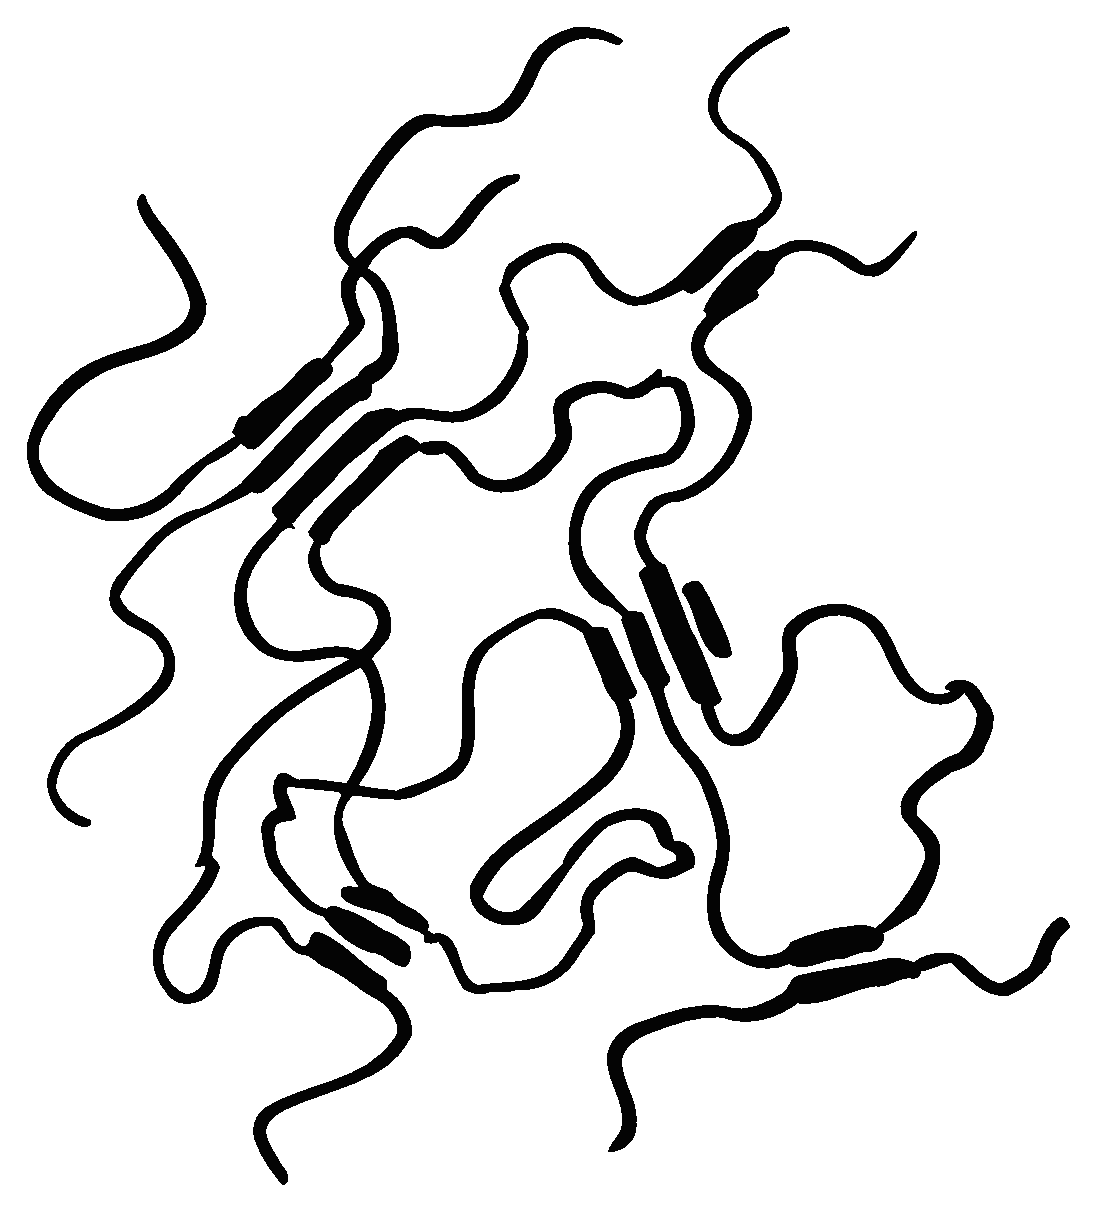
\includegraphics[scale=0.27]{CrystTPE_CC0.pdf}
	\caption{Exemple de structure pour un élastomère thermoplastique avec segments cristallins (image libre de droits)}
	\label{fig:structure_TPECryst}
\end{figure}

\FloatBarrier
En ce qui concerne la soudure des élastomères, très peu de références existent, encore moins en ce qui concerne le soudage entre des matériaux mixtes. 
Un article de Hollande documente le soudage par ultrasons de tissus imprégnés de polyuréthane thermoplastique, où les soudures présentent les fibres et l'élastomère comme étant deux phases distinctes l'une de l'autre sans diffusion entre celles-ci \cite{Hollande1998}. 
À ce jour, aucun article ne traite du soudage où se produit une diffusion de chaines d'élastomère thermoplastique dans un autre polymère thermoplastique. 

La solution actuellement employée par ArianeGroup pour les composites à matrice thermodurcissable ne requiert pas l'emploi d'un élastomère thermoplastique. 
Dans ce cas, puisqu'il n'est pas nécessaire de les souder ou de les fondre de nouveau, un élastomère conventionnel avec des chaines réticulées peut rencontrer les requis techniques. 
Ainsi, un copolymère butadiène-acrylonitrile est présentement collé avec des colles époxydes. 
Les requis techniques du projet sont calqués sur les performances mécaniques de cette solution. 
Cependant, cette méthode présente plusieurs faiblesses. 
Tout d'abord, elle impose un temps de fabrication très long en raison du temps de réticulation de l'époxy. 
Ensuite, elle est très sensible à la présence de contaminants et nécessite une préparation de surface méticuleuse. 
Finalement, la solution employée n'est pas robuste, puisqu'elle ne produit pas des résultats totalement répétables en raison de sa sensibilité aux contaminants. 

\section{Enjeux scientifiques}

La revue de la littérature a permis d'identifier une série d'enjeux scientifiques directement liés à cette thèse. 
Tout d'abord, en considérant le contexte du projet qui vise la réalisation d'une jonction entre un composite thermoplastique et un élastomère, il sera nécessaire de considérer la problématique de la compatibilité des polymères et de la diffusion des chaines entre plusieurs matériaux dissimilaires. 

Également, en considérant le nanocomposite qui sera employé pour le procédé de soudage par résistance, on peut cerner deux enjeux. 
En premier lieu, il y a une grande incertitude quant au comportement électrique d'un nanocomposite conducteur caractérisé à l'état solide une fois rendu à l'état fondu. 
On peut se questionner à savoir si les contacts entre les nanotubes seront maintenus durant la fonte ou si ces liaisons seront affectées et que la conductivité électrique sera perdue. 
En second lieu, lors de l'élaboration d'un nanocomposite conducteur, il peut devenir important de bien contrôler les processus de distribution et de dispersion des charges conductrices dans la matrice polymérique. 
  % Revue de littérature.
\selectlanguage{french}
\Chapter{OBJECTIFS DE LA RECHERCHE}\label{sec:Objectifs}

\section{Analyse des lacunes dans les connaissances actuelles}

Le procédé de soudure par résistance des composites thermoplastiques avec un élément chauffant en acier inoxydable est un procédé simple qui offre de bonnes propriétés mécaniques et qui peut facilement être mis à l'échelle. 
Sa faiblesse réside dans le manque d'interaction entre le polymère et l'élément chauffant. 
Celle-ci peut être contournée de deux façons \begin{inparaenum}[a)]
	\item en effectuant des traitements de surface permettant d'augmenter l'adhésion entre la matrice et l'acier inoxydable ou 
	\item en changeant la nature de l'élément chauffant. 
\end{inparaenum}
En ce qui concerne la première solution, des travaux de recherche sont en cours à l'École de technologie supérieure afin d'explorer cette option. 
Pour la seconde solution, un élément chauffant constitué d'un nanocomposite conducteur pourrait être employé. 
Le polymère de la matrice de ce nanocomposite devra pouvoir diffuser au travers du polymère des adhérents et l'ajout de particules conductrices le rendra conducteur. 
Ainsi, le nanocomposite développé servirait à la fois d'élément chauffant et offrira une zone riche en polymère pour produire une soudure. 
Bien entendu, la conductivité électrique du nanocomposite ne pourra certainement pas atteindre celle de l'élément chauffant en acier inoxydable. 
Sa plus faible conductivité fera en sorte que le nanocomposite aura une résistance électrique beaucoup plus élevée. 
Il sera alors possible de tirer parti de cette résistance pour utiliser le nanocomposite comme élément chauffant. 
Cette solution est inexplorée dans les articles précédemment publiés. 

Un autre trou existe dans les écrits recensés en rapport à la possibilité de souder un élastomère thermoplastique avec un autre polymère rigide. 
Dans le meilleur des cas, un mélange biphasique avec un élastomère et un autre polymère est utilisé dans une jonction, mais sans obtenir de diffusion entre les phases \cite{Hollande1998}. 
Aucun cas documenté de soudage mixte entre un élastomère et un autre polymère n'a été trouvé. 

Ainsi, nous pouvons détecter deux besoins de recherche. 
Tout d'abord en ce qui concerne la production d'un élément chauffant nanocomposite permettant la soudure par résistance de composites thermoplastiques. 
En second lieu, par l'obtention d'une soudure mixte avec un élastomère. 

\section{Objectifs}

En considérant l'ensemble des connaissances publiées et des besoins du partenaire industriel, voici la liste des objectifs sur lesquels se concentreront ces travaux. 

\begin{enumerate}
	\item Concevoir un élément chauffant nanocomposite conducteur en tenant compte des propriétés électriques et thermiques nécessaires au procédé de soudage par résistance. 
	\item Développer un procédé de soudage par résistance avec un élément chauffant nanocomposite entre deux adhérents en composite à matrice thermoplastique. 
	\item Établir une fenêtre d'opération pour le soudage par résistance avec un élément chauffant nanocomposite entre deux adhérents en composite à matrice thermoplastique. 
	\item Développer un procédé de soudage par résistance avec un élément chauffant nanocomposite entre un adhérent en composite à matrice thermoplastique et un adhérent en élastomère thermoplastique. 
\end{enumerate}

\section{Cibles de performance}

Afin d'évaluer l'atteinte des objectifs et pour aides dans la sélection des matériaux, ArianeGroup a fourni des cibles de performance calquées sur les caractéristiques de la solution actuelle pour les composites à matrice thermodurcissable. 
Voici deux des principaux requis techniques concernant la jonction soudée. 

\begin{enumerate}
	\item Résistance en cisaillement supérieure à \SI{14}{\mega\pascal}. 
	\item Rupture cohésive de l'élastomère. 
\end{enumerate}

\section{Contenu des chapitres \ref{sec:Theme1} à \ref{sec:Theme3}}

Le contenu des prochains chapitres est une application directe des objectifs qui viennent d'être établis. 
En tout premier lieu, le chapitre \ref{sec:Theme1} présentera un article traitant du développement du nanocomposite ainsi que la preuve de concept nécessaire pour démontrer la possibilité de l'utiliser comme élément chauffant lors d'un soudage par résistance. 
En second lieu, le chapitre \ref{sec:Theme2} présente un article traitant de l'amélioration des performances du procédé par l'emploi d'un modèle numérique par éléments finis afin de cibler une fenêtre d'opération plus précise et augmenter la résistance mécanique des joints soudés. 
En dernier lieu, le chapitre \ref{sec:Theme3} présente les travaux ayant été menés afin de développer une jonction flexible intégrant un élastomère thermoplastique.   % Description des objectifs généraux et spécifiques ainsi qu'une brève description des thèmes qui suivent
\Chapter{ARTICLE 1 : RESISTANCE WELDING OF THERMOPLASTIC COMPOSITES WITH A NANOCOMPOSITE HEATING ELEMENT}\label{sec:Theme1}

\hyphenation{COMSOL na-no-com-po-si-te na-no-com-po-si-tes}

\selectlanguage{french}
\section{Introduction}

Cet article présente les travaux ayant mené au développement d'un élément chauffant nanocomposite pour le soudage résistif de composites thermoplastiques. La planification des travaux, la réalisation des expériences, l'analyse des résultats et la rédaction de cet article ont été réalisés par David Brassard. Martine Dubé et Jason R. Tavares ont supervisé l'ensemble des travaux et ont contribué à la révision de l'article. 

\textbf{Auteurs} : David Brassard, Martine Dubé et Jason R. Tavares

\textbf{Article publié dans la revue} : \textit{Composites Part B: Engineering}, Volume 165, 15 May 2019, pages 779-784

\textbf{URL} : \url{https://doi.org/10.1016/j.compositesb.2019.02.038}

\textbf{Mots-clés} : Resistance welding; Polymer–matrix composites (PMCs); Thermoplastic resin; Joints/joining

\selectlanguage{english}

\section{Abstract}

In this study, we propose a new heating element (HE) for the resistance welding of thermoplastic composites. 
This HE is made of polyetherimide (PEI), rendered electrically conductive by the addition of 10\% wt. multi-wall carbon nanotubes (MWCNT) (conductivity of \SI{0.79}{\siemens\per\cm}).
The new HE were successfully used to weld carbon fibre/poly(ether ether ketone) (CF/PEEK) laminates in a single lap shear configuration, leading to a lap shear strength of up to \SI{19.6}{\mega\pascal}.
Observations of the fracture surfaces revealed a cohesive failure mode within the nanocomposite HE and non-uniform heating over the weld area. 
It is believed that PEI/MWCNT HE present an interesting alternative to current HE, although more work is needed to improve the temperature homogeneity over the weld area.
	
%%%%%%%%%%%%%%%%%%%%%%%%%%%%%%%%%%%%%%%%%%%%%%%%%%%%%%%%%%%%%%%%%
\section{Introduction}
%%%%%%%%%%%%%%%%%%%%%%%%%%%%%%%%%%%%%%%%%%%%%%%%%%%%%%%%%%%%%%%%%

The current fierce competition in the space industry is putting a strong downward pressure on the launch cost of satellites. 
New processes and materials are needed to reduce launchers' weight and cost. 
Fibre reinforced polymers are commonly used to achieve weight reduction. 
Currently, thermoset polymers dominate the market for composite matrices but thermoplastic composites (TPC) are attracting the attention of the industry \cite{CompositeWorldSloan2018} because of their higher impact resistance, increased production rates, superior recyclability and higher environmental resistance \cite{cogswell1992}. 
Moreover, a distinct advantage of thermoplastics over thermosets is their ability to be joined by welding instead of adhesive bonding or mechanical fastening. 

Different welding processes have been developed for various applications and joint geometry. 
Resistance welding, induction welding and ultrasonic welding are a few of the processes used for joining TPC. 
To weld the adherents (i.e. the parts to be joined) through traditional resistance welding (Fig. \ref{fig:welding_jig}a), heat is generated by a porous and electrically conductive heating element located at the weld interface and connected to a power source. 
An electrical current is applied to the heating element to generate heat. 
The connection between the power supply and the heating element is generally established by copper connectors that are clamped at a predetermined distance from the edges of the adherents (the so-called “clamping distance”). 
During the welding process, pressure is applied to the weld stack to achieve intimate contact and to promote autohesion during the melting and consolidation phases. 

\begin{figure}[h]
	\centering
	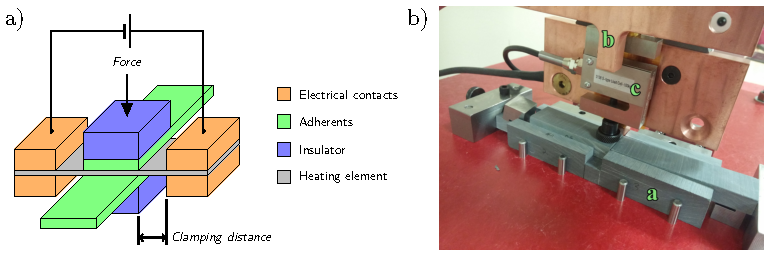
\includegraphics[width=130mm]{Fig1.pdf}
	\caption{Resistance welding jig a) Resistance welding main components, b) Ceramic insulators [a], copper electrodes [b] and load cell [c] \cite{Brassard2018_figshare_article1}}
	\label{fig:welding_jig}
\end{figure}

\FloatBarrier
The first heating elements that were used for the resistance welding process were made of carbon fibre  \cite{Ageorges2000a,houghton1984bonding,Eveno1988}.
Poor weld reproducibility and problematic electrical connections between the electrodes and the carbon fibres caused scaling issues \cite{McKnight1997}. 
These shortcomings led to the use of stainless steel (SS) mesh heating elements that improved the consistency of the process \cite{Hou1999a}.

The lap shear strength (LSS) obtained from single lap shear (SLS) specimens and failure modes are commonly reported to evaluate the performance of welded joints. 
For samples welded with SS heating elements under suboptimal conditions, adhesive failure (ADH) between the mesh and the polymer or between the polymer and the adherents is obtained. 
These failure modes can be accompanied by tearing of the mesh. 
Under good welding conditions, light-fiber-tear failure (LFT), often accompanied by mesh tearing, is observed \cite{Shi2014}. 
Failure modes and LSS are dependent on the fibre nature and orientation within the adherents \cite{Shi2013a}. 
For materials with lower performances, such as glass fibre and polyetherimide (GF/PEI), failure occurs in the adherents, but for high performance and stiffer materials, such as unidirectional carbon fibre and poly(ether ether ketone) (CF/PEEK) laminates, damage occurs in the heating element with little to no damage to the adherents \cite{Dube2015}. 
The variations in the failure modes indicate that poor adhesive bonding between the polymer and the SS mesh can be a limiting factor under certain circumstances \cite{Dube2007,Dube2012a,Dube2009a,Shi2014,Shi2015a}. 
An increase in the fraction of open area of the SS mesh, to a certain extent, improves LSS. 
Concurrently, some concerns were expressed regarding the weight penalty of SS meshes \cite{Stavrov2005a}. 

Players from the space industry are looking at alternative heating elements.  
Their target is a low-density material that is not affected by corrosion. 
A conductive polymer-based nanocomposite heating element, compatible with the adherents, could serve as that alternative and provide good interfacial bonding. 
Such nanocomposites are formed by dispersing conductive nanoparticles (typically metal or carbon) into a polymer matrix. 
The electrical properties of nanocomposites depend, among other things, on the intrinsic properties of the nanoparticles, their mass fraction, surface modifications, and the mixing method employed. 
This was illustrated by Bauhofer et al., who showed that the same kinds of particles can produce nanocomposites with widely different properties \cite{Bauhofer2009}. 
For applications such as resistance welding, we seek a conductivity sufficiently low to generate heat through the Joule effect but high enough to prevent current leakage through the adherents. 

For traditional resistance welding of high performance TPC parts made of CF/PEEK, PEI is sometimes used to provide a resin-rich region at the weld interface. 
The miscibility of PEI in PEEK \cite{Crevecoeur1991} also improves the bonding between the adherents to attain good mechanical performances. 
By using PEI for the matrix of the nanocomposite, we hypothesize that we could take advantage of that miscibility and obtain a nanocomposite heating element suitable for resistance welding of CF/PEEK laminates while welding at temperatures lower than the melting temperature of PEEK (in a similar way to the Thermabond process \cite{Smiley1991a}). 
This novel heating element would be almost entirely miscible within the matrix of the composite and does not leave metallic elements within the weld. 
Furthermore, the MWCNT/PEI coefficient of thermal expansion is better matched with that of CF/PEEK composites than pure PEI with a metallic insert. 
Therefore, it is believed that thermal residual stress can be reduced by the use of this nanocomposite HE. 

This article presents the development of this new heating element for resistance welding of TPC with a PEI-based conductive nanocomposite. 
Joule heating of the nanocomposite is validated with a sample heating element. 
This new heating element is then used to join CF/PEEK adherents and their mechanical performance is evaluated by single lap shear tests. 

%%%%%%%%%%%%%%%%%%%%%%%%%%%%%%%%%%%%%%%%%%%%%%%%%%%%%%%%%%%%%%%%%
\section{Methodology}
%%%%%%%%%%%%%%%%%%%%%%%%%%%%%%%%%%%%%%%%%%%%%%%%%%%%%%%%%%%%%%%%%

%%%%%%%%%%%%%%%%%%%%%%%%%%%%%%%%%%%%%%%%%%%%%%%%%%%%%%%%%%%%%%
\subsection{Materials}
%%%%%%%%%%%%%%%%%%%%%%%%%%%%%%%%%%%%%%%%%%%%%%%%%%%%%%%%%%%%%%

\subsubsection{Polymer and Nanocomposite}

The polymer used for the heating element development was PEI (CAS 61128-46-9) pellets ordered from Sigma Aldrich. 
PEI pellets had a melt index of \SI{18}{\gram} per \SI{10}{\minute} at \SI{337}{\celsius} with a mass of \SI{6.6}{\kilogram}. 
GPC/SEC measurements of the molecular weight for this PEI gave a $M_n$ of \SI{15.0}{\kg\per\mol} and a $M_w$ of \SI{21.6}{\kg\per\mol}. 

The conductive nanoparticles consisted of dry powdered MWCNTs, produced by combustion chemical vapour deposition (CCVD), purchased from Raymor Industries. 
They had outer diameters in the range of \SIrange{10}{20}{\nano\metre}, lengths from \SIrange{1}{12}{\micro\metre} and purity of at least 99\%.

Initial batches of nanocomposites with 5\%, 10\% and 15\% wt. of MWCNTs were produced with a DSM Xplore 5~cc twin-screw micro-compounder. 
Polymer pellets were introduced along with the MWCNTs and internally mixed by the recirculation circuit.
The resulting extruded wire was cut into pellets that were mixed and fed a second time to produce a uniform mix for each batch. 
The pellets were hot-pressed to produce \SI{1.6}{\mm} thick flat samples to measure their electrical conductivity.  

The electrical conductivity of the PEI nanocomposites, at 5\%, 10\% and 15\% wt. of MWCNTs, was measured with the four-point probe technique. 
A probe manufactured by Jandel engineering was mounted on a resistivity test rig from A\&M Fell Ltd. and connected to an acquisition system composed of a Keithley 220 programmable current source and a Hewlett Packard 34401A multimeter. 
The tungsten carbide probes had a diameter of \SI{0.4}{\mm}, a radius of \SI{100}{\um} and a spacing of \SI{1}{\mm}. 

The final batch of nanocomposite with 10\% wt. of MWCNTs, for the manufacturing of the heating elements, was produced in a twin-screw extruder and processed at \SI{340}{\celsius}. 
Polymer pellets were introduced along with the MWCNTs. 
The extruded wire was cut into small pellets, mixed thoroughly and fed back into the extruder two other times to obtain a uniform composition. 
The final wire was cut into pellets prior to further processing. 
Flat PEI nanocomposite heating elements, with a 10\% mass fraction of MWCNTs, were produced by hot pressing pellets into \SI{0.5}{\milli\metre} thick films and cutting them into rectangles of \SI{12.7 x 55}{\milli\metre}. 

\subsubsection{Composite}

The TPC adherents were produced by compression moulding CF/PEEK pre-impregnated plies to form unidirectional (UD) composite laminates and cutting them to dimensions (\SI{25.4 x 101.6}{\milli\metre} ), with an abrasive saw, according to ASTM D5868 - 01(2014). 
In agreement with the supplier’s recommendations, the stacks of plies were heated to \SI{390}{\celsius} under a pressure of \SI{0.25}{\MPa}. 
The pressure was then increased to \SI{1}{\MPa} for \SI{30}{\minute} to consolidate the laminate before cooling it back to room temperature in about \SI{60}{\minute}. 
The pressure was maintained during the cooling phase. 

%%%%%%%%%%%%%%%%%%%%%%%%%%%%%%%%%%%%%%%%%%%%%%%%%%%%%%%%%%%%%%
\subsection{Joule Heating of a Nanocomposite Heating Element}
%%%%%%%%%%%%%%%%%%%%%%%%%%%%%%%%%%%%%%%%%%%%%%%%%%%%%%%%%%%%%%

Prior to the welding tests, a simple validation of the heating elements was devised. 
A \SI{0.5}{\milli\metre} thick PEI heating element was installed in the welding setup and connected to electrodes \SI{25}{\mm} spaced apart. 
A constant DC voltage was then applied for \SI{45}{\s}. 
A FLIR T420 infrared camera was used to record the surface temperature distribution once an electrical current was applied. 

%%%%%%%%%%%%%%%%%%%%%%%%%%%%%%%%%%%%%%%%%%%%%%%%%%%%%%%%%%%%%%
\subsection{Welding Experiments}
%%%%%%%%%%%%%%%%%%%%%%%%%%%%%%%%%%%%%%%%%%%%%%%%%%%%%%%%%%%%%%

A computer-controlled resistance welding jig was built to weld single lap shear specimens with an overlap of \SI{12.7}{\milli\metre} and a width of \SI{25.4}{\milli\metre} (Fig. \ref{fig:welding_jig}). 
Two copper electrodes were used to connect the power source to the nanocomposite heating element. 
Three pneumatic actuators applied constant pressure over the two electrodes and the welding zone, while the nanocomposite was kept between two composite adherents. 
The electrodes where connected to the heating element, on each side of the laminate (Fig. \ref{fig:welding_jig}a) with the proper clamping distance for each test. 
Electrical power was supplied by a \SI{10}{\kW} programmable DC power source series XR from Magna-Power capable of providing up to \SI{160}{\volt} and \SI{60}{\ampere}. 
The power source can be driven as a constant voltage source, constant current source or with custom power profiles. 
A modulation scheme was configured to allow the source to operate with a constant power output. 
In this mode of operation, the source adjusts its output current based on the voltage applied and keeps a constant power output, disregarding variations in the resistance of the heating element. 

For the welding experiments, electrical parameters were set so as to closely mimic conditions that are observed during traditional resistance welding of TPC. 
The initial voltage setting for constant voltage operation was calculated based on a specific power of \SI{350}{\kW\per\square\metre} and the electrical resistance of the heating element. 

Prior to welding, the surfaces of the adherents and the nanocomposite were cleaned with acetone. 
Once the heating element and adherents were installed in the welding jig, a contact pressure of 2.4 MPa was applied by the electrodes on the heating element, to minimize contact resistance. 
Over the weld area, a third actuator applied a constant pressure of \SI{1}{\MPa} during the whole welding process. 
It was previously demonstrated, for traditional resistance welding, that pressures close to \SI{1}{\MPa} are able to produce welds with good mechanical properties by promoting intimate contact, necessary for polymer chain diffusion at the interfaces, while preventing void formation due to excessive polymer flow out of the weld \cite{Ageorges2000a, Dube2007, Shi2014}. 
Type K thermocouples, located on the ceramic above the welded zone, monitored the temperature during the welding process (Fig. \ref{fig:thermocouple}a). 
The thermocouples could not be installed directly on the nanocomposite heating element, as their presence altered the heat transfer mechanisms within the weld and Kapton\textregistered \ tape was not sufficient prevent electrical interference. 
The first thermocouple was located slightly off centre at \SI{14}{\milli\metre} from the edge of the adherent at the centreline of the overlap. 
The second thermocouple was also located on the centreline, but \SI{2.5}{\milli\metre} away from the edge of the adherent. 
These two locations served as proxy to approximate the temperature within the weld. 
Closer to the heating element, a higher temperature is expected. 
Aside from the operating mode for the power source, the clamping distance and the duration of the welding process were the main factors taken into account during the welding tests. 

\begin{figure}[b!]
	\centering
	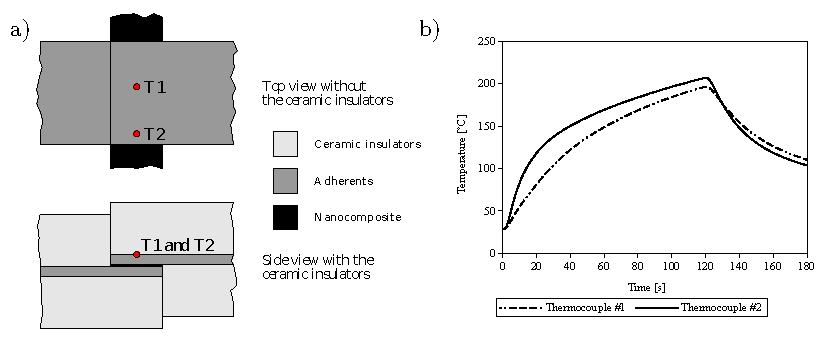
\includegraphics[width=140mm]{Fig2.pdf}
	\caption{Thermocouples locations and measurements a) Location of the thermocouples during the welding process, b) Evolution of the temperature during the welding process at \SI{350}{\kilo\watt\per\square\metre} for \SI{120}{\second} \cite{Brassard2018_figshare_article1}}
	\label{fig:thermocouple}
\end{figure}

\FloatBarrier
%%%%%%%%%%%%%%%%%%%%%%%%%%%%%%%%%%%%%%%%%%%%%%%%%%%%%%%%%%%%%%
\subsection{Characterization of welded joints}
%%%%%%%%%%%%%%%%%%%%%%%%%%%%%%%%%%%%%%%%%%%%%%%%%%%%%%%%%%%%%%

The LSS of each weld was evaluated with a SLS test as per ASTM D5868 – 01(2014) with an MTS Alliance RF/200 testing machine. 
Subsequently, fractography analysis was carried out with ImageJ. 
In this analysis, dividing the area of the welded zone by the total area gave the percentage of welded area. 
Both faces of the fractured specimens were evaluated to get an average measure for each sample. 
The failure modes obtained were classified and reported as per ASTM D5573 – 99(2012). 

%%%%%%%%%%%%%%%%%%%%%%%%%%%%%%%%%%%%%%%%%%%%%%%%%%%%%%%%%%%%%%
\subsection{FTIR Analysis}
%%%%%%%%%%%%%%%%%%%%%%%%%%%%%%%%%%%%%%%%%%%%%%%%%%%%%%%%%%%%%%

FTIR spectra were collected to validate the absence of thermal degradation due to the welding process. 
A Nicolet iS5 FTIR Spectrometer equipped with an iD5 attenuated total reflectance (ATR) module was used to collect spectra from the virgin PEI pellets and PEI nanocomposite films before welding, and PEI nanocomposite on the fracture surfaces after SLS tests. 
Spectra for CF/PEEK adherents were also collected to serve as reference.  

%%%%%%%%%%%%%%%%%%%%%%%%%%%%%%%%%%%%%%%%%%%%%%%%%%%%%%%%%%%%%%%%%
\section{Results and Discussion}
%%%%%%%%%%%%%%%%%%%%%%%%%%%%%%%%%%%%%%%%%%%%%%%%%%%%%%%%%%%%%%%%% 

%%%%%%%%%%%%%%%%%%%%%%%%%%%%%%%%%%%%%%%%%%%%%%%%%%%%%%%%%%%%%%
\subsection{Electrical Conductivity of the Nanocomposites}
%%%%%%%%%%%%%%%%%%%%%%%%%%%%%%%%%%%%%%%%%%%%%%%%%%%%%%%%%%%%%%

The electrical conductivity of PEI nanocomposites with 5\%, 10\% and 15\% wt. MWCNTs was \SIlist[multi-part-units = single]{0.27(08);0.79(06);0.92(30)}{\siemens\per\cm}, respectively. 
It was decided that the marginal gain in conductivity between 10\% and 15\% wt. MWCNTs was not worth the increased cost and production problems associated with high particle loading (such as increased viscosity and brittleness). 
Thus, a PEI nanocomposite with 10\% wt. MWCNTs was retained for manufacturing heating elements. 

%%%%%%%%%%%%%%%%%%%%%%%%%%%%%%%%%%%%%%%%%%%%%%%%%%%%%%%%%%%%%%
\subsection{Micro-Mechanical Simulations of Joule Heating}
%%%%%%%%%%%%%%%%%%%%%%%%%%%%%%%%%%%%%%%%%%%%%%%%%%%%%%%%%%%%%%

During the initial development of the nanocomposite, finite element models were developed using COMSOL Mul\-ti\-phy\-sics\-\textregistered \ to evaluate the contribution of the three main heating mechanisms inside the nanocomposite heating element (i.e. Joule heating of MWCNTs, from the concentration of charges at the contact points between MWCNTs and of the matrix between MWCNTs) and verify that the polymer will not undergo thermal degradation.  
A set of three continuum micromechanic models presenting different contact topologies were used to assess the relative contribution of each heating mechanism to the global heating phenomena within a conductive nanocomposite. 
The uniform temperature fields observed at the constituent level led to the conclusion that under normal operating conditions, local thermal degradation should not occur within the nanocomposite during the welding process and that Joule heating is the dominant mode of heat generation. 
The complete methodology and results for these simulations are included as Supplementary Information. 

%%%%%%%%%%%%%%%%%%%%%%%%%%%%%%%%%%%%%%%%%%%%%%%%%%%%%%%%%%%%%%
\subsection{Joule Heating of a Nanocomposite Heating Element}
%%%%%%%%%%%%%%%%%%%%%%%%%%%%%%%%%%%%%%%%%%%%%%%%%%%%%%%%%%%%%%

At the beginning of the Joule Heating tests, a uniform temperature field is observed in the nanocomposite (Fig. \ref{fig:results_lab}). 
For longer test durations, the copper electrodes are acting as heat sinks at the edges of the heating element causing a measurable temperature gradient (Fig. \ref{fig:results_lab}). 
It was possible to control the surface temperature of the heating element with a variation of the voltage (Tab. \ref{tab:results_lab}). 
The voltages applied during this test were limited to stay below the glass transition temperature of PEI at \SI{217}{\celsius}. 
These results validate the Joule heating behaviour of the nanocomposite heating element. 

\begin{figure}[htb]
	\centering
	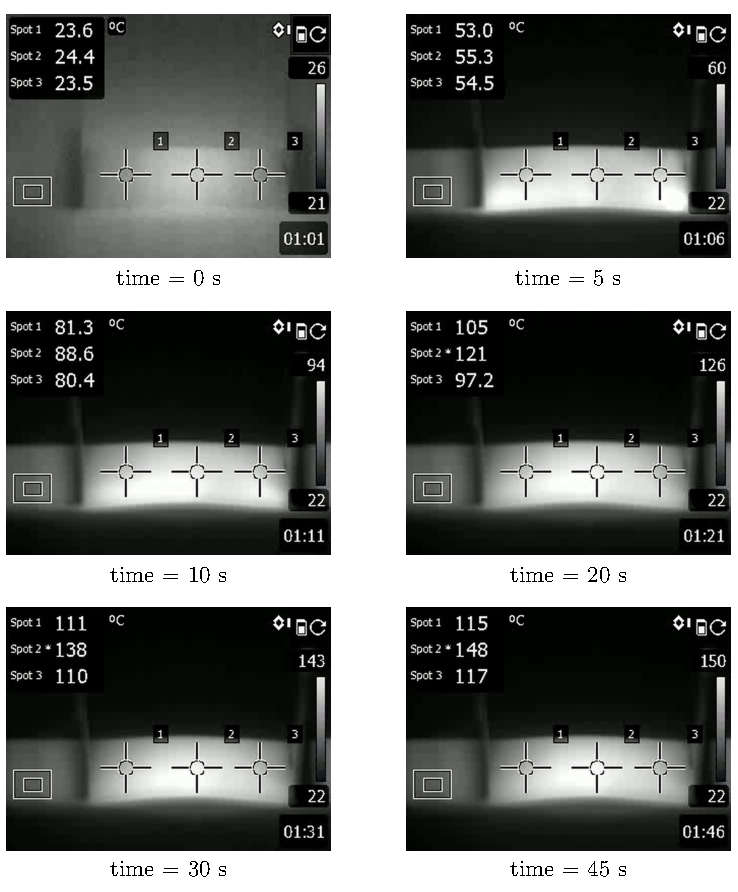
\includegraphics[width=125mm]{Fig3.pdf}
	\caption{Thermography of a heating element during the experimental validation under a DC electrical field of \SI{800}{\volt\per\metre} \cite{Brassard2018_figshare_article1}}
	\label{fig:results_lab}
\end{figure}

\begin{table}[htb]
	\centering
	\caption{Electrical results from the experimental validation, the current at \SI{30}{\volt} could not be measured due to melting of the heating element}
	\begin{tabular}{@{}lrrr@{}}
		\toprule
		Voltage 				& Electric							& Maximum  				& Current\\ 
		& field								& surface 				& \\ 
		& 										& temperature 			& \\
		{[}\si{\volt}{]} 	& {[}\si{\volt\per\metre}{]} 	& {[}\si{\celsius}{]}	& {[}\si{\ampere}{]}\\ \midrule
		10 						& 400									& 44 						& 0.10 \\
		15						& 600									& 97 						& 0.16 \\
		20 						& 800									& 155 						& 0.23 \\
		25 						& 1000									& 223 						& 0.32 \\
		30 						& 1200									& \textgreater 270 	& N/A \\ \bottomrule
	\end{tabular}
	
	\label{tab:results_lab}
\end{table}

\FloatBarrier
%%%%%%%%%%%%%%%%%%%%%%%%%%%%%%%%%%%%%%%%%%%%%%%%%%%%%%%%%%%%%%
\subsection{Welding Experiments}
%%%%%%%%%%%%%%%%%%%%%%%%%%%%%%%%%%%%%%%%%%%%%%%%%%%%%%%%%%%%%%

Small geometric variations of the nanocomposite heating elements (thickness and width) introduced variations of the electrical resistance. 
Because of this variation, operation under constant voltage conditions achieved poor reproducibility between initial welding tests and was not investigated further. 
Operation under constant power yielded significant improvements in the consistency of welding results, avoiding the effect introduced by the heating element electrical resistance variation. 

\subsubsection{Constant power welding}

Tests were carried out at a specific power of \SI{350}{\kW\per\square\metre} with a constant pressure of \SI{1}{\MPa} on the weld. 
Clamping distances of \SIlist{0;1;1.5}{\mm} and welding times of \SIlist{60;70;90;120}{\s} were investigated. 
Three samples were produced for each welding condition. 
The LSS along with the average fraction of welded areas are reported in Table \ref{tab:SLS_and_fractography_results}. 

\begin{table}[h]
	\centering
	\caption{LSS and fractography analysis reported as average values $\pm$ standard deviation \cite{Brassard2018_figshare_article1}}
	\begin{tabular}{@{}lllcccc@{}}
		\toprule
		Clamping distance & Values      &                 &                     \multicolumn{4}{c}{Time}                      \\
		{[}\si{\mm}{]}    &             &                 &                 \multicolumn{4}{c}{{[}\si{\s}{]}}                 \\
		                  &             &                 &       60       &       70       &       90       &      120       \\ \midrule
		0                 & LSS         & {[}\si{\MPa}{]} &                &                &                & \num{14.5(13)} \\
		                  & Welded area & {[}\%{]}        &                &                &                &  \num{85(2)}   \\
		1                 & LSS         & {[}\si{\MPa}{]} &                &                &                & \num{13.0(44)} \\
		                  & Welded area & {[}\%{]}        &                &                &                &  \num{83(7)}   \\
		1.5               & LSS         & {[}\si{\MPa}{]} & \num{16.4(78)} & \num{18.6(20)} & \num{15.5(38)} & \num{19.6(35)} \\
		                  & Welded area & {[}\%{]}        &  \num{57(20)}  &  \num{74(10)}  &  \num{87(1)}   &  \num{78(2)}   \\ \bottomrule
	\end{tabular}
	\label{tab:SLS_and_fractography_results}
\end{table}

\FloatBarrier
Average LSS from \SI{13}{\MPa} up to \SI{19.6}{\MPa} were obtained. 
Longer weld times allowed the nanocomposite to melt and bind with the adherents over a larger fraction of the welded zone. 
From the conditions tested, applying current for \SI{120}{\s} with a clamping distance of \SI{1.5}{\mm} yielded the best LSS results. 

Cohesive failure within the nanocomposite was the primary mode of failure observed for samples welded under constant power with UD composite adherents.
Some adhesive failure on the edges of the heating element was also observed. 
Samples welded for \SI{60}{\s} with a clamping distance of \SI{1.5}{\mm} presented a higher fraction of adhesive failure. 
The zone where cohesive failure is observed had thinner width at the centre of the weld (Fig. \ref{fig:fracture_surface}a). 
For welding times of \SI{90}{\s} and longer, the thinner middle section is absent from the results and only cohesive failure of the nanocomposite is present (Fig. \ref{fig:fracture_surface}b). 

\begin{figure}[h]
	\centering
	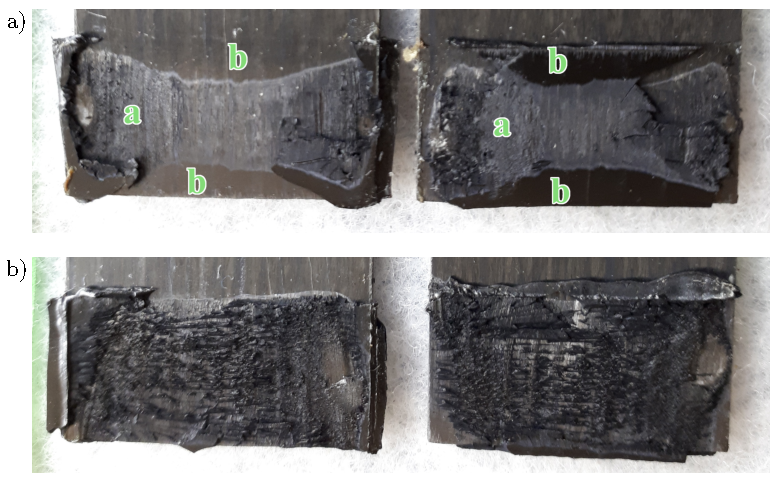
\includegraphics[width=132mm]{Fig4.pdf}
	\caption{Fracture surface of specimens welded at \SI{350}{\kW\per\square\metre} with \SI{1.5}{\mm} clamping distance a) Cohesive failure with a thinner section in the middle [a] and adhesive failure on the sides [b] in a sample welded for \SI{70}{\s}, b) Mostly cohesive failure in a sample welded for \SI{90}{\s} \cite{Brassard2018_figshare_article1}}
	\label{fig:fracture_surface}
\end{figure}

\FloatBarrier
Temperature monitoring during the welding process of a sample with a clamping distance of \SI{1.5}{\mm} showed temperature variations between the centre and the edge of the weld (Fig. \ref{fig:thermocouple}b).
For this specimen, the edge effect resulted in a \SI{10}{\celsius} higher temperature on the top surface at the edge of the adherent, compared to the center. 
This difference was caused by a clamping distance that was too large. 
Models will be required to evaluate if the gradients in the weld are larger or smaller than the gradient from the thermocouples located at the top of the adherents. 
Nonetheless, the temperature gradient between the center and the edges was not large enough to lead to observable thermal degradation in the fractography results, either on the edges (from a too large clamping distances) or at the centre of the weld (from a too small clamping distances). 
It was previously demonstrated that the clamping distance has an important effect on the heat transfer at the edge of the weld \cite{Talbot2013}. 

Although the LSS obtained with the nanocomposite heating element are lower than the best results reported in the literature for traditional resistance welding, successful welds were obtained and key optimization parameters were identified for future work. 
A better understanding and control of those parameters will allow the production of higher performance joints. 
The key parameters are : \begin{enumerate}
	\item the reduced toughness of the nanocomposite due to the addition of a high fraction of MWCNTs,
	\item the incomplete polymer melting in the welded zone due to edge effects and
	\item the thinner middle section in the welded zone leading to stress concentration at the edge. 
\end{enumerate}
Tensile tests on dogbones made from the nanocomposite showed that the addition of 10\% wt. fraction of MWCNTs caused a 40\% reduction of the tensile strength compared to virgin PEI. 
Plasticizers could be used to reduce the negative impact of MWCNTs but the composition of the nanocomposite will need to be balanced so as to still provide a sufficient electrical conductivity. 
Improving the control of the welding process (clamping distance, time and power density) will reduce the temperature gradients within the welded zone and provide a better wetting over the whole surface of the joint. 

\subsection{FTIR results}

When comparing the FTIR spectra of PEI nanocomposites before and after the welding process, no signs of degradation could be noted (see Supplementary Information). 
The characteristic peeks for \ch{CH3}, \ch{CH} and \ch{C=O} in PEI were left unchanged by the welding process. 

%%%%%%%%%%%%%%%%%%%%%%%%%%%%%%%%%%%%%%%%%%%%%%%%%%%%%%%%%%%%%%%%%
\section{Conclusion}
%%%%%%%%%%%%%%%%%%%%%%%%%%%%%%%%%%%%%%%%%%%%%%%%%%%%%%%%%%%%%%%%%

Through this work, we have demonstrated that a PEI/MWCNT-based nanocomposite heating element could be used for resistance welding of TPCs. 
An experimental validation using a PEI/MWCNT flat heating element subjected to a DC electric field showed uniform heating. 
Resistance welding using the PEI/MWCNT heating element in a custom-built welding jig joined CF/PEEK UD panels with LSS up to \SI{19.6}{\MPa}. 
Good bonding to the adherents is supported by the cohesive failure mode observed, and no important thermal degradation is measured by FTIR tests. 
Future work will focus on improving the temperature uniformity in the weld and improving the toughness of the nanocomposite heating element.

%%%%%%%%%%%%%%%%%%%%%%%%%%%%%%%%%%%%%%%%%%%%%%%%%%%%%%%%%%%%%%%%%
\section{Acknowledgements}
%%%%%%%%%%%%%%%%%%%%%%%%%%%%%%%%%%%%%%%%%%%%%%%%%%%%%%%%%%%%%%%%%

This work was supported by ArianeGroup and CREPEC. 
The authors also thank Prof. G.S. Patience for the use of the thermal imaging camera and Prof. D. Therriault for access to the microcompounder. 
             % Premier thème (Doctorat) ou "Détails de la Solution" (Maîtrise).
\Chapter{ARTICLE 2 : MODELLING RESISTANCE WELDING OF THERMOPLASTIC COMPOSITES WITH A NANOCOMPOSITE HEATING ELEMENT}\label{sec:Theme2}

\selectlanguage{french}
\section{Introduction}

Cet article présente les travaux de modélisation du soudage résistif de composites thermopastiques avec un élément chauffant nanocomposite. Ces travaux avaient pour but d'optimiser les performances mécaniques des joints et établir une fenêtre d'opération. La planification des travaux, la réalisation des expériences, l'analyse des résultats et la rédaction de cet article ont été réalisés par David Brassard. Martine Dubé et Jason R. Tavares ont supervisés l'ensemble des travaux et ont contribués à la révision de l'article. 

\textbf{Auteurs} : David Brassard, Martine Dubé et Jason R. Tavares

\textbf{Article soumis dans la revue} : Composites Part B: Engineering

\textbf{Date de soumission} : 7 octobre 2019

\textbf{Mots clés} : Resistance welding; Finite element analysis (FEA); Thermoplastic resin; \\ Joints/joining

\selectlanguage{english}

\section{Abstract}

Electrically conductive nanocomposite heating elements are being developed as a complement to traditional carbon fibre or stainless steel heating elements in resistance welding of thermoplastic composites. 
Here we present the development of a finite element model of the resistance welding process with these new heating elements, from which we establish a process window for high quality welded joints. 
The finite element model results were validated experimentally and a lap shear strength improvement of 28\% is reported relative to previously published results. 
Fractography analysis of the broken joints revealed a thin-layer cohesive failure mode due to the brittleness of the nanocomposite heating elements. 

%%%%%%%%%%%%%%%%%%%%%%%%%%%%%%%%%%%%%%%%%%%%%%%%%%%%%%%%%%%%%%%%%
\section{Introduction}
%%%%%%%%%%%%%%%%%%%%%%%%%%%%%%%%%%%%%%%%%%%%%%%%%%%%%%%%%%%%%%%%%

The use of thermoplastic composite (TPC) materials is rising \cite{Mathijsen2016} and these materials now find applications in wind turbine and aerospace industries \cite{Penumadu2019}. 
Their short processing cycle, improved impact resistance, end-of-life recyclability and chemical stability \cite{cogswell1992} make them good candidates for lightweight structural components compared to traditional thermoset resins. 
A major difference between thermosets and thermoplastics is the methods to join parts together: while adhesive bonding and mechanical assembly is the norm for thermoset composites, assemblies of TPCs are preferably produced by welding together individual components. 
This is achieved by localized heating of the weld zone through resistance, induction or ultrasonic welding. 
During resistance welding, the weld zone temperature increases via Joule heating of a resistive heating element (HE) located between the adherents \cite{Ageorges2001a,Stavrov2005a,Dube2007c,Shi2014,Brassard2019a,Eveno1988} (Fig. \ref{fig:2_Fig1}). 
This process offers good mechanical performance and short processing times of the order of minutes, and can be achieved with HE such as carbon fibre plies \cite{Eveno1988}, stainless steel (SS) meshes \cite{Stavrov2005a,Dube2007c,Shi2014} or, more recently, an electrically conductive nanocomposite polymer \cite{Brassard2019a}. 

\begin{figure}[ht]
	\center
	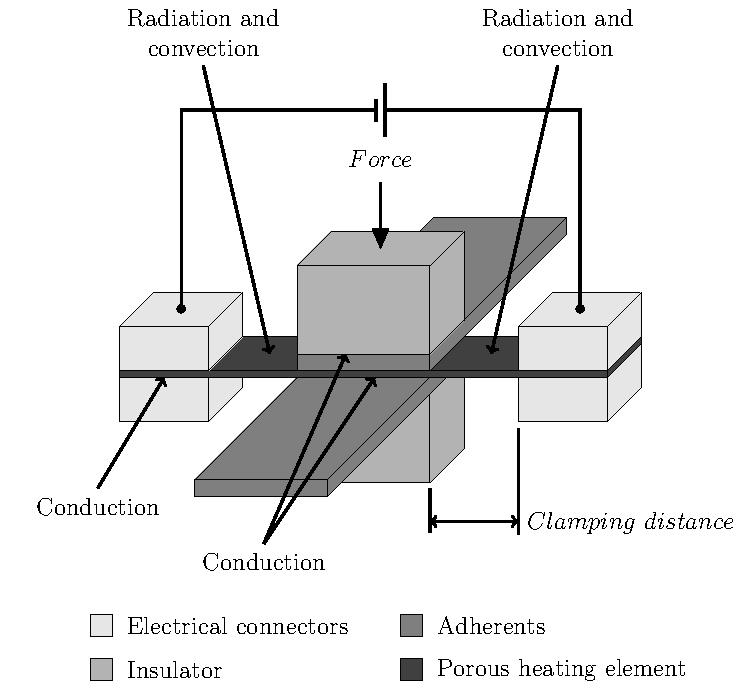
\includegraphics[scale=1]{2_Fig1}
	\caption{Schematic view of the resistance welding process highlighting local thermal transport mechanisms \cite{Brassard2019b}}
	\label{fig:2_Fig1}
\end{figure} 

It was recently shown that an electrically conductive nanocomposite polymer HE can successfully weld unidirectional (UD) carbon fibre reinforced PEEK (CF/PEEK) composite adherents \cite{Brassard2019a}. 
While this proof-of-concept illustrated how the new HE could complement SS meshes and carbon fibre HE, the effects of the welding parameters on the weld quality were not thoroughly explored. 
The development of a processing window is needed to assess the full capabilities of the nanocomposite HE. 

The main parameters controlling the resistance welding process are the power density (electrical power divided by the heating element area), duration, welding pressure, geometry of the components of the jig holding the adherents and the properties of the materials used as thermal insulators. 
Good control of the heating parameters is required to keep the heat-affected zone (HAZ) as close as possible to the bonding surfaces to avoid deconsolidation and fibre movements \cite{Stavrov2005a}. 
The power density and process duration affect the size and shape of the HAZ by controlling the rate and amount of energy dissipated within the weld, while pressure on the laminates prevents the formation of porosity from deconsolidation of the plies \cite{Shi2017}. 
For a given welding jig configuration, the clamping distance and the dimensions and nature of the electrodes dictate edge effects, which are caused by the sharp transition in the heat dissipation mechanism of the HE from conduction in the weld and adherents to radiation and potentially convection outside the weld as illustrated in Fig. \ref{fig:2_Fig1} \cite{Ageorges2001b}. 
Edge effects can have a strong impact on the temperature distribution within the weld. 
Inappropriate adjustment of the clamping distance may lead to incomplete welding or degradation at the edges \cite{Talbot2013}. 
Finally, the thermal properties and geometry of the insulators will have a strong impact on optimal processing parameters, making those parameters dependant on the design of the welding jig. 
Going from an experimental jig to a production setup requires careful considerations and a deep understanding of the welding process. 

A process window that compounds all these effects cannot be obtained solely through physical experiments, because key processing information is unavailable. 
Namely, the inability to install thermocouples within the weld without disturbing the process limits the ability to measure the temperature at the interface when using a nanocomposite HE. 
However, information gained through preliminary experiments can be used to help developing a finite element model of resistance welding with a nanocomposite HE, which will in turn guide subsequent exploration of the welding parameters. 

Therefore, this article presents the development and validation of a transient finite element model for resistance welding of thermoplastic composites with a nanocomposite HE. 
This model is subsequently used to predict good welding conditions and establish a processing window leading to improved mechanical performances. 

%%%%%%%%%%%%%%%%%%%%%%%%%%%%%%%%%%%%%%%%%%%%%%%%%%%%%%%%%%%%%%%%%
\section{Methodology}
%%%%%%%%%%%%%%%%%%%%%%%%%%%%%%%%%%%%%%%%%%%%%%%%%%%%%%%%%%%%%%%%%

%%%%%%%%%%%%%%%%%%%%%%%%%%%%%%%%%%%%%%%%%%%%%%%%%%%%%%%%%%%%%%
\subsection{Resistance welding finite element model}
%%%%%%%%%%%%%%%%%%%%%%%%%%%%%%%%%%%%%%%%%%%%%%%%%%%%%%%%%%%%%%

A transient finite element model of the resistance welding process is developed with the COMSOL Multiphysics\textregistered \ software. 
The model evaluates the effects of welding parameters on the temperature distribution and profile in the joint over time with the goal of establishing a processing window leading to good weld quality and mechanical performance based on these results. 
This model evaluates the electrical field in the electrodes and nanocomposite HE, Joule heating of the nanocomposite HE, heat transfer in the solids, heat dissipation through convection and radiation and thermal contact conductance between critical components. 
The geometry of the components is detailed in Fig. \ref{fig:2_Fig2}. 
The gaps identified in the geometry were \mbox{0.1\,mm}.

\begin{figure}[h!]
	\center
	\resizebox{0.9\textwidth}{!}{
	%\usetikzlibrary{3d}
\begin{tikzpicture}[scale=0.11]
\LARGE

%Overlap distance
\def \overlap{12.7}

%Clamping distance
\def \cdistance{1.5}

%Thermal discontinuities gap
\def \gap{0.75}

%Electrodes dimensions
\def \telectrode{0.5*25.4}
\def \helectrode{2*25.4}

%Dimensions des adhérent
\def \ladherent{4*25.4}
\def \tadherent{2.1}
\def \wadherent{25.4}

%Nanocomposite dimensions
\def \tnano{0.55}
\def \lnano{54.8}
\def \wnano{\overlap}

%Ceramic insulators
\def \tceramic{0.5*25.4}
\def \hceramic{25.4}

%Composite base plate
\def \tcompositeplate{25.4}
\def \lcompositeplate{10*25.4}
\def \wcompositeplate{6*25.4}

%Position et taille des annotations
\def \dia{4.25}
\def \detailscale{5}
\def \legend{12.7}
\def \distcotation{2.5}

%Colour palette for colourbliness
\definecolor{orange}{rgb}{0.902,0.624,0}
\definecolor{skyblue}{rgb}{0.337,0.7058,0.9137}
\definecolor{bluegreen}{rgb}{0,0.6196,0.4509}
\definecolor{yellow}{rgb}{0.9411,0.8941,0.2588}
\definecolor{blue}{rgb}{0,0.4471,0.6980}
\definecolor{vermillion}{rgb}{0.8353,0.3686,0}
\definecolor{purple}{rgb}{0.8,0.4745,0.6549}

%\def \colelectrode{orange}
%\def \colceramic{skyblue}l
%\def \coladherent{bluegreen}
%\def \colnano{yellow}
%\def \colbase{vermillion}

\def \colelectrode{black!25}
\def \colceramic{black!45}
\def \coladherent{black!68}
\def \colnano{black}
\def \colbase{black!5}

%GF composite base
\begin{scope}[,line join=round]
	\draw[black,fill=\colbase] (0,-\tadherent-\tceramic,0) -- ++(0,0,0.5*\wcompositeplate) -- ++(-0.5*\lcompositeplate,0,0) -- ++(0,0,-\wcompositeplate)  -- ++(\lcompositeplate,0,0)   -- ++(0,0,0.5*\wcompositeplate) -- cycle; %Top face
	\draw[black,fill=\colbase] (-0.5*\lcompositeplate,-\tadherent-\tceramic,0.5*\wcompositeplate) -- ++(0,-\tcompositeplate,0) -- ++(0.5*\lcompositeplate,0,0) -- ++(0,\tcompositeplate,0)  -- cycle; %Bottom left
	\draw[black,fill=\colbase] (0,-\tadherent-\tceramic,0.5*\wcompositeplate) -- ++(0,-\tcompositeplate,0) -- ++(0,0,-0.5*\wcompositeplate) -- ++(0,\tcompositeplate,0)  -- cycle; %Bottom middle left
	\draw[black,fill=\colbase] (0,-\tadherent-\tceramic,0) -- ++(0,-\tcompositeplate,0) -- ++(0.5*\lcompositeplate,0,0) -- ++(0,\tcompositeplate,0)  -- cycle; %Bottom middle right
	\draw[black,fill=\colbase] (0.5*\lcompositeplate,-\tadherent-\tceramic,0) -- ++(0,-\tcompositeplate,0) -- ++(0,0,-0.5*\wcompositeplate) -- ++(0,\tcompositeplate,0)  -- cycle; %Bottom right
\end{scope}

%Lower adherent
\begin{scope}[shift={(-0.5*\overlap,-\tadherent,0.5*\wadherent)},line join=round]
	\draw[black,fill=\coladherent] (0,0,0) -- ++(0.5*\overlap,0,0) --  ++(0,\tadherent,0)  -- ++(-0.5*\overlap,0,0)  -- cycle; % Front 1
	\draw[black,fill=\coladherent] (0.5*\overlap,0,-0.5*\wadherent) -- ++(\ladherent-0.5*\overlap,0,0) --  ++(0,\tadherent,0)  -- ++(-\ladherent+0.5*\overlap,0,0)  -- cycle; % Front 2
	\draw[black,fill=\coladherent] (0,\tadherent,0) -- ++(0.5*\overlap,0,0) -- ++(0,0,-0.5*\wadherent) --++ (\ladherent-0.5*\overlap,0,0) -- ++(0,0,-0.5*\wadherent) -- ++(-\ladherent,0,0)  -- cycle; % Top
	\draw[black,fill=\coladherent] (0.5*\overlap,0,0) -- ++(0,\tadherent,0) -- ++(0,0,-0.5*\wadherent) -- ++(0,-\tadherent,0)  -- cycle; % Side 1
	\draw[black,fill=\coladherent] (\ladherent,0,-0.5*\wadherent) -- ++(0,\tadherent,0) -- ++(0,0,-0.5*\wadherent) -- ++(0,-\tadherent,0)  -- cycle; % Side 2
\end{scope}

%Nanocomposite
\begin{scope}[shift={(-0.5*\overlap,0,0.5*\lnano)},line join=round]
	\draw[black,fill=\colnano] (0,0,0) -- ++(0.5*\overlap,0,0) --  ++(0,\tnano,0)  -- ++(-0.5*\overlap,0,0)  -- cycle; % Front 1
	\draw[black,fill=\colnano] (0.5*\overlap,0,-0.5*\lnano) -- ++(0.5*\overlap,0,0) --  ++(0,\tnano,0)  -- ++(-0.5*\overlap,0,0)  -- cycle; % Front 2
	\draw[black,fill=\colnano] (0,\tnano,0) -- ++(0.5*\overlap,0,0) -- ++(0,0,-0.5*\lnano) --++ (0.5*\overlap,0,0) -- ++(0,0,-0.5*\lnano) -- ++(-\overlap,0,0)  -- cycle; % Top
	\draw[black,fill=\colnano] (0.5*\overlap,0,0) -- ++(0,\tnano,0) -- ++(0,0,-0.5*\lnano) -- ++(0,-\tnano,0)  -- cycle; % Side 1
	\draw[black,fill=\colnano] (\overlap,0,-0.5*\lnano) -- ++(0,\tnano,0) -- ++(0,0,-0.5*\lnano) -- ++(0,-\tnano,0)  -- cycle; % Side 2
\end{scope}

%Back electrode
\begin{scope}[shift={(-0.5*\overlap,\tnano,-0.5*\lnano+\telectrode)},line join=round]
	\draw[black,fill=\colelectrode] (0,0,0) -- ++(\overlap,0,0) --  ++(0,\helectrode,0)  -- ++(-\overlap,0,0)  -- cycle; % Front
	\draw[black,fill=\colelectrode] (0,\helectrode,0) -- ++(\overlap,0,0) -- ++(0,0,-\telectrode) -- ++(-\overlap,0,0)  -- cycle; % Top
	\draw[black,fill=\colelectrode] (\overlap,0,0) -- ++(0,\helectrode,0) -- ++(0,0,-\telectrode) -- ++(0,-\helectrode,0)  -- cycle; % Side
\end{scope}

%Upper adherent
\begin{scope}[shift={(-\ladherent+0.5*\overlap,\tnano,0.5*\wadherent)},line join=round]
\draw[black,fill=\coladherent] (0,0,0) -- ++(\ladherent-0.5*\overlap,0,0) --  ++(0,\tadherent,0)  -- ++(-\ladherent+0.5*\overlap,0,0)  -- cycle; % Front 1
	\draw[black,fill=\coladherent] (\ladherent-0.5*\overlap,0,-0.5*\wadherent) -- ++(0.5*\overlap,0,0) --  ++(0,\tadherent,0)  -- ++(-0.5*\overlap,0,0)  -- cycle; % Front 2
	\draw[black,fill=\coladherent] (0,\tadherent,0) -- ++(\ladherent-0.5*\overlap,0,0) -- ++(0,0,-0.5*\wadherent) --++ (0.5*\overlap,0,0) -- ++(0,0,-0.5*\wadherent) -- ++(-\ladherent,0,0)  -- cycle; % Top
	\draw[black,fill=\coladherent] (\ladherent-0.5*\overlap,0,0) -- ++(0,\tadherent,0) -- ++(0,0,-0.5*\wadherent) -- ++(0,-\tadherent,0)  -- cycle; % Side 1
	\draw[black,fill=\coladherent] (\ladherent,0,-0.5*\wadherent) -- ++(0,\tadherent,0) -- ++(0,0,-0.5*\wadherent) -- ++(0,-\tadherent,0)  -- cycle; % Side 2
\end{scope}

%Upper ceramic 1
\begin{scope}[shift={(-\ladherent+0.5*\overlap,\tnano+\tadherent,0.5*\wadherent)},line join=round]
\draw[black,fill=\colceramic] (0,0,0) -- ++(\ladherent-0.5*\overlap,0,0) --  ++(0,\tceramic,0)  -- ++(-\ladherent+0.5*\overlap,0,0)  -- cycle; % Front 1
	\draw[black,fill=\colceramic] (\ladherent-0.5*\overlap,0,-0.5*\wadherent) -- ++(0.5*\overlap,0,0) --  ++(0,\tceramic,0)  -- ++(-0.5*\overlap,0,0)  -- cycle; % Front 2
	\draw[black,fill=\colceramic] (0,\tceramic,0) -- ++(\ladherent-0.5*\overlap,0,0) -- ++(0,0,-0.5*\wadherent) --++ (0.5*\overlap,0,0) -- ++(0,0,-0.5*\wadherent) -- ++(-\ladherent,0,0)  -- cycle; % Top
	\draw[black,fill=\colceramic] (\ladherent-0.5*\overlap,0,0) -- ++(0,\tceramic,0) -- ++(0,0,-0.5*\wadherent) -- ++(0,-\tceramic,0)  -- cycle; % Side 1
	\draw[black,fill=\colceramic] (\ladherent,0,-0.5*\wadherent) -- ++(0,\tceramic,0) -- ++(0,0,-0.5*\wadherent) -- ++(0,-\tceramic,0)  -- cycle; % Side 2
\end{scope}

%Lower ceramic
\begin{scope}[shift={(-\ladherent+0.5*\overlap,-\tadherent-\tceramic,0.5*\wadherent+\tceramic)},line join=round]
	\draw[black,fill=\colceramic] (0,0,0) -- ++(\ladherent-0.5*\overlap,0,0) --  ++(0,\tceramic+\tadherent,0)  -- ++(-0.5*\overlap,0,0)  -- ++(0,\hceramic-\tceramic-\tadherent,0)  -- ++(-\ladherent+\overlap,0,0) -- cycle; % Front 1
	\draw[black,fill=\colceramic] (\ladherent-0.5*\overlap,0,-0.5*\wadherent-\tceramic) -- ++(\ladherent-0.5*\overlap,0,0) --  ++(0,\tceramic,0)  -- ++(-\ladherent+0.5*\overlap,0,0)  -- cycle; % Front 2
	\draw[black,fill=\colceramic] (2*\ladherent-\overlap,\tceramic,-\wadherent-\tceramic-\gap) -- ++(-\overlap,0,0) --  ++(0,\tceramic,0)  -- ++(\overlap,0,0)  -- cycle; % Front 3
	\draw[black,fill=\colceramic] (0,\hceramic,0) -- ++(\ladherent-\overlap,0,0) -- ++(0,0,-\tceramic+\gap) --++ (-\ladherent+\overlap,0,0) -- ++(0,0,\tceramic-\gap)  -- cycle; % Top
	\draw[black,fill=\colceramic] (2*\ladherent-\overlap,\tceramic,-0.5*\wadherent-\tceramic) -- ++(-\overlap,0,0) -- ++(0,0,-0.5*\wadherent-\gap) --++ (\overlap,0,0) -- ++(0,0,0.5*\wadherent+\gap)  -- cycle; % Top 2
	\draw[black,fill=\colceramic] (\ladherent+\gap,\hceramic,-\tceramic-\gap-\wadherent) -- ++(\ladherent-\overlap-\gap,0,0) -- ++(0,0,-\tceramic,0) --++ (-\ladherent+\overlap+\gap,0,0)  -- cycle; % Top 3
	\draw[black,fill=\colceramic] (\ladherent-\overlap,\tceramic+\tadherent-\gap,-\tceramic+\cdistance) -- ++(0.5*\overlap,0,0) -- ++(0,0,-\cdistance) --++ (-0.5*\overlap,0,0)  -- cycle; % Top 4 (gap)
	\draw[black,fill=\colceramic] (\ladherent-0.5*\overlap,0,0) -- ++(0,\tceramic+\tadherent,0) -- ++(0,0,-\tceramic+\cdistance) -- ++(0,-\gap,0) -- ++(0,0,-\cdistance) -- ++(0,-\tadherent+\gap,0) -- ++(0,0,-0.5*\wadherent) -- ++(0,-\tceramic,0)  -- cycle; % Side 1
	\draw[black,fill=\colceramic] (2*\ladherent-\overlap,0,-0.5*\wadherent-\tceramic) -- ++(0,\tceramic,0) -- ++(0,0,-0.5*\wadherent-\gap) -- ++(0,\hceramic-\tceramic,0) -- ++(0,0,-\tceramic) -- ++(0,-\hceramic,0) -- cycle; % Side 2
\end{scope}

%Lower adherent redraw
\begin{scope}[shift={(-0.5*\overlap,-\tadherent,0.5*\wadherent)},line join=round]
	\draw[black,fill=\coladherent] (0.5*\overlap,0,-0.5*\wadherent) -- ++(\ladherent-0.5*\overlap,0,0) --  ++(0,\tadherent,0)  -- ++(-\ladherent+0.5*\overlap,0,0)  -- cycle; % Front 2
	\draw[black,fill=\coladherent] (\ladherent,0,-0.5*\wadherent) -- ++(0,\tadherent,0) -- ++(0,0,-0.5*\wadherent) -- ++(0,-\tadherent,0)  -- cycle; % Side 2
\end{scope}

%Nanocomposite redraw
\begin{scope}[shift={(-0.5*\overlap,0,0.5*\lnano)},line join=round]
	\draw[black,fill=\colnano] (0,0,0) -- ++(0.5*\overlap,0,0) --  ++(0,\tnano,0)  -- ++(-0.5*\overlap,0,0)  -- cycle; % Front 1
	\draw[black,fill=\colnano] (0.5*\overlap,0,0) -- ++(0,\tnano,0) -- ++(0,0,-0.5*\lnano) -- ++(0,-\tnano,0)  -- cycle; % Side 1
\end{scope}

%Upper ceramic 2
\begin{scope}[shift={(0.5*\overlap+\gap,0,-00)},line join=round]
	\draw[black,fill=\colceramic] (0,0,0) -- ++(\ladherent-\overlap-\gap,0,0) --  ++(0,\tceramic,0)  -- ++(-\ladherent+\overlap+\gap,0,0)  -- cycle; % Front
	\draw[black,fill=\colceramic] (0,\tceramic,0) -- ++(\ladherent-\overlap-\gap,0,0) -- ++(0,0,-\telectrode) -- ++(-\ladherent+\overlap+\gap,0,0)  -- cycle; % Top
	\draw[black,fill=\colceramic] (\ladherent-\overlap-\gap,0,0) -- ++(0,\tceramic,0) -- ++(0,0,-\telectrode) -- ++(0,-\tceramic,0)  -- cycle; % Side
\end{scope}

%Front electrode
\begin{scope}[shift={(-0.5*\overlap,\tnano,0.5*\lnano)},line join=round]
	\draw[black,fill=\colelectrode] (0,0,0) -- ++(0.5*\overlap,0,0) --  ++(0,\helectrode,0)  -- ++(-0.5*\overlap,0,0)  -- cycle; % Front
	\draw[black,fill=\colelectrode] (0,\helectrode,0) -- ++(0.5*\overlap,0,0) -- ++(0,0,-\telectrode) -- ++(-0.5*\overlap,0,0)  -- cycle; % Top
	\draw[black,fill=\colelectrode] (0.5*\overlap,0,0) -- ++(0,\helectrode,0) -- ++(0,0,-\telectrode) -- ++(0,-\helectrode,0)  -- cycle; % Side
\end{scope}

%Electrical circuit
\begin{scope}[shift={(0,0)},line join=round]
	\draw[ultra thick, black] (0,\helectrode+\tnano,0.5*\wadherent+0.5*\telectrode+\cdistance) -- ++(0,0.5*\helectrode,0) -- ++(0,0,-0.5*\wadherent-0.5*\telectrode-\cdistance+2) -- ++(0,5,0) -- ++(0,-10,0); 
	\draw[ultra thick, black] (0,\helectrode+\tnano,-0.5*\wadherent-0.5*\telectrode-\cdistance) -- ++(0,0.5*\helectrode,0) -- ++(0,0,0.5*\wadherent+0.5*\telectrode+\cdistance-2) -- ++(0,10,0) -- ++(0,-20,0); 
\end{scope}

%Scale
\begin{scope}[shift={(0,0)},line join=round]
	\draw[ultra thick, black, <->] (-0.5*\lcompositeplate,-\tnano-\tadherent-\tceramic-0.5*\tcompositeplate,0.5*\wcompositeplate) -- ++(0.5*\lcompositeplate,0,0) node[pos=.5, below] {75 mm}; 
	\draw[] ((-0.5*\lcompositeplate-10,-\tnano-\tadherent-\tceramic-\tcompositeplate-3,0.5*\wcompositeplate) node [below right] {\LARGE{\textbf{Gaps are not to scale}}} ;
\end{scope}

%Circle for detail A
\begin{scope}[shift={(-0.5*\overlap,0.5*\tnano,0.5*\lnano)}]
	\draw[very thick, black] (0,0,0) circle[radius=\dia] node[left=0.1*\dia] {\textbf{\LARGE{A}}};
\end{scope}

%Circle for detail B
\begin{scope}[shift={(0.5*\overlap+0.5*\gap,0.5*\tnano,0)}]
	\draw[very thick, black] (0,0,0) circle[radius=\dia] node[below=0.1*\dia] {\textbf{\LARGE{B}}};
\end{scope}

%Circle for detail C
\begin{scope}[canvas is zy plane at x=0]
	\draw[very thick, black] (0.5*\wadherent+0.5*\cdistance,0.5*\tnano) circle[radius=\dia] node[below=0.1*\dia] {\textbf{\LARGE{C}}};
\end{scope}

%Circle for detail D
\begin{scope}[canvas is zy plane at x=\ladherent-0.5*\overlap]
	\draw[very thick, black] (-0.5*\wadherent-0.5*\gap,-0.5*\tadherent) circle[radius=\dia] node[below=0.1*\dia] {\textbf{\LARGE{D}}};
\end{scope}

%Detail view A
\begin{scope}[,shift={(-5*25.4,2.5*25.4)}]
\begin{scope}[scale=\detailscale]
	\draw[very thick, black] (0,0) circle[radius=\dia];
	\draw[] (0,-\dia) node[below=0.1*\dia]{\LARGE{\textbf{Detail A}}};
	\begin{scope}
		\clip (0,0) circle[radius=\dia];
		%\draw[very thick, black,fill=\coladherent] (-\gap,+0.5*\tnano) -- ++(\gap,0) --  ++(0,\tadherent)  -- ++(-\gap,0)  -- cycle;
		\draw[very thick, black,fill=\colnano] (0,-0.5*\tnano) -- ++(0.5*\overlap,0) --  ++(0,\tnano)  -- ++(-0.5*\overlap,0)  -- cycle;
		\draw[very thick, black,fill=\colelectrode] (0,+0.5*\tnano) -- ++(0.5*\overlap,0) --  ++(0,\helectrode)  -- ++(-0.5*\overlap,0)  -- cycle;
		\draw[very thick, black,fill=\colceramic] (0-\gap,-0.5*\tnano) -- ++(0.5*\overlap,0) --  ++(0,-\tceramic)  -- ++(-\overlap,0)  -- ++(0,2*\tceramic) -- ++(0.5*\overlap,0) -- cycle;
		%\draw[very thick, black,fill=\colceramic] (0-\gap,0.5*\tnano+\tadherent) -- ++(\gap,0) --  ++(0,\tceramic)  -- ++(-\gap,0) -- cycle;
	\end{scope}
	\draw[very thick, black] (-\gap,\dia+0.25) -- ++ (0,\distcotation);
	\draw[very thick, black] (0,\dia+0.25) -- ++ (0,\distcotation);
	\draw [very thick, black, <->] (-\gap,\dia+0.25+0.5*\distcotation) -- ++ (\gap,0) node[right] {\LARGE Gap};
\end{scope}
\end{scope}

%Detail view B
\begin{scope}[,shift={(-2.25*25.4,2.5*25.4)}]
\begin{scope}[scale=\detailscale]
	\draw[very thick, black] (0,0) circle[radius=\dia];
	\draw[] (0,-\dia) node[below=0.1*\dia]{\LARGE{\textbf{Detail B}}};
	\begin{scope}
		\clip (0,0) circle[radius=\dia];
		\draw[very thick, black,fill=\colnano] (-\overlap-0.5*\gap,-0.5*\tnano) -- ++(\overlap,0) --  ++(0,\tnano)  -- ++(-\overlap,0)  -- cycle;
		\draw[very thick, black,fill=\coladherent] (-\overlap-0.5*\gap,-0.5*\tnano-\tadherent) -- ++(\wadherent,0) --  ++(0,\tadherent)  -- ++(-\wadherent,0)  -- cycle;
		\draw[very thick, black,fill=\coladherent] (-\overlap-0.5*\gap,0.5*\tnano) -- ++(\overlap,0) --  ++(0,\tadherent)  -- ++(-\overlap,0)  -- cycle;
		\draw[very thick, black,fill=\colceramic] (-\overlap,-0.5*\tnano-\tadherent) -- ++(2*\overlap,0) --  ++(0,-\tadherent) --  ++(-2*\overlap,0) -- cycle;
		\draw[very thick, black,fill=\colceramic] (-\overlap-0.5*\gap,0.5*\tnano+\tadherent) -- ++(\overlap,0) --  ++(0,\tadherent)  -- ++(-\overlap,0)  -- cycle;
		\draw[very thick, black,fill=\colceramic] (0.5*\gap,-0.5*\tnano) -- ++(\wadherent,0) --  ++(0,\tceramic)  -- ++(-\wadherent,0) -- cycle;
	\end{scope}
	\draw[very thick, black] (-0.5*\gap,\dia+0.25) -- ++ (0,\distcotation);
	\draw[very thick, black] (0.5*\gap,\dia+0.25) -- ++ (0,\distcotation);
	\draw [very thick, black, <->] (-0.5*\gap,\dia+0.25+0.5*\distcotation) -- ++ (\gap,0) node[right] {\LARGE Gap};
\end{scope}
\end{scope}

%Detail view C
\begin{scope}[,shift={(2*25.4,2.5*25.4)}]
\begin{scope}[scale=\detailscale]
	\draw[very thick, black] (0,0) circle[radius=\dia];
	\draw[] (0,-\dia) node[below=0.1*\dia]{\LARGE{\textbf{Detail C}}};
	\begin{scope}
		\clip (0,0) circle[radius=\dia];
		\draw[very thick, black,fill=\colnano] (-0.5*\cdistance-\telectrode,-0.5*\tnano) -- ++(\lnano,0) --  ++(0,\tnano)  -- ++(-\lnano,0)  -- cycle;
		\draw[very thick, black,fill=\coladherent] (\gap+0.5*\cdistance,-0.5*\tnano-\tadherent) -- ++(\wadherent,0) --  ++(0,\tadherent)  -- ++(-\wadherent,0)  -- cycle;
		\draw[very thick, black,fill=\coladherent] (\gap+0.5*\cdistance,0.5*\tnano) -- ++(\wadherent,0) --  ++(0,\tadherent)  -- ++(-\wadherent,0)  -- cycle;
		\draw[very thick, black,fill=\colelectrode] (-0.5*\cdistance-\telectrode,0.5*\tnano) -- ++(\telectrode,0) --  ++(0,\helectrode)  -- ++(-\telectrode,0)  -- cycle;
		\draw[very thick, black,fill=\colceramic] (-0.5*\cdistance-\telectrode,-0.5*\tnano) -- ++(\tceramic,0) --  ++(0,-\gap) --  ++(\cdistance,0) -- ++(0,-\tadherent+\gap)  -- ++(0.5*\wadherent,0) -- ++(0,-\tceramic) -- cycle;
		\draw[very thick, black,fill=\colceramic] (\gap+0.5*\cdistance,0.5*\tnano+\tadherent) -- ++(\wadherent,0) --  ++(0,\tceramic)  -- ++(-\wadherent,0) -- cycle;
	\end{scope}
	\draw[very thick, black] (0.5*\cdistance+\gap,\dia+0.25) -- ++ (0,1.5*\distcotation);
	\draw[very thick, black] (0.5*\cdistance,\dia+0.25) -- ++ (0,0.75*\distcotation);
	\draw[very thick, black] (-0.5*\cdistance,\dia+0.25) -- ++ (0,1.5*\distcotation);
	\draw [very thick, black, <->] (0.5*\cdistance,\dia+0.25+0.5*\distcotation) -- ++ (\gap,0) node[right] {\LARGE Gap};
	\draw [very thick, black, <->] (-0.5*\cdistance,\dia+0.25+\distcotation) -- ++ (\cdistance+\gap,0) node[right] {\LARGE Clamping distance};
	\draw [very thick, black] (\dia+0.25,-0.5*\tnano)-- ++ (\distcotation,0);
	\draw [very thick, black] (\dia+0.25,-0.5*\tnano-\gap)-- ++ (\distcotation,0);
	\draw [very thick, black, <->] (\dia+0.25+0.5*\distcotation,-0.5*\tnano-\gap) -- ++ (0,\gap) node[above] {\LARGE Gap};
\end{scope}
\end{scope}

%Detail view D
\begin{scope}[,shift={(5*25.4,2.5*25.4)}]
\begin{scope}[scale=\detailscale]
	\draw[very thick, black] (0,0) circle[radius=\dia];
	\draw[] (0,-\dia) node[below=0.1*\dia]{\LARGE{\textbf{Detail D}}};
	\begin{scope}
		\clip (0,0) circle[radius=\dia];
		\draw[very thick, black,fill=\coladherent] (-\wadherent-0.5*\gap,-0.5*\tadherent) -- ++(\wadherent,0) --  ++(0,\tadherent)  -- ++(-\wadherent,0)  -- cycle;
		\draw[very thick, black,fill=\colceramic] (-\overlap-0.5*\gap,0.5*\tadherent) -- ++(\overlap,0) --  ++(0,\tceramic)  -- ++(-\overlap,0)  -- cycle;
		\draw[very thick, black,fill=\colceramic] (-\wadherent,-0.5*\tadherent-\tceramic) -- ++(2*\wadherent+0.5*\gap,0) --  ++(0,2*\tceramic)  -- ++(-\wadherent,0) -- ++(0,-\tceramic)  -- ++(-\wadherent,0) -- cycle;
	\end{scope}
	\draw[very thick, black] (-0.5*\gap,\dia+0.25) -- ++ (0,\distcotation);
	\draw[very thick, black] (0.5*\gap,\dia+0.25) -- ++ (0,\distcotation);
	\draw [very thick, black, <->] (-0.5*\gap,\dia+0.25+0.5*\distcotation) -- ++ (\gap,0) node[right] {\LARGE Gap};
\end{scope}
\end{scope}

% %Origin Tikz
% \begin{scope}[shift={(25,-50,0)}]
% 	\draw[fill=black] (0,0,0,) circle (0.15);
% 	\draw [very thick, black, ->] (0,0,0) -- ++(0,0,25.4) node [below left]{\ \Huge Z};
% 	\draw [very thick, black, ->] (0,0,0) -- ++(25.4,0,0) node [right]{\ \Huge X};
% 	\draw [very thick, black, ->] (0,0,0) -- ++(0,25.4,0) node [above]{\ \Huge Y};
% \end{scope}

%%%%%%%%%%%%%%%%%%%%%%%%
% Redraw of the small isometric view
%%%%%%%%%%%%%%%%%%%%%%%%

\begin{scope}[shift={(-85,-125)},line join=round]
\begin{scope}[scale=0.75]
	
	%Lower adherent
	\begin{scope}[shift={(-0.5*\overlap,-\tadherent,0.5*\wadherent)},line join=round]
		\draw[black,fill=\coladherent] (0,0,0) -- ++(\ladherent,0,0) --  ++(0,\tadherent,0)  -- ++(-\ladherent,0,0)  -- cycle; % Front 1
		\draw[black,fill=\coladherent] (0,\tadherent,0) -- ++(\ladherent,0,0) -- ++(0,0,-\wadherent) -- ++(-\ladherent,0,0)  -- cycle; % Top
		\draw[black,fill=\coladherent] (\ladherent,0,0) -- ++(0,\tadherent,0) -- ++(0,0,-\wadherent) -- ++(0,-\tadherent,0)  -- cycle; % Side 1
	\end{scope}
	
	%Nanocomposite
	\begin{scope}[shift={(-0.5*\overlap,0,0.5*\lnano)},line join=round]
		\draw[black,fill=\colnano] (0,0,0) -- ++(\overlap,0,0) --  ++(0,\tnano,0)  -- ++(-\overlap,0,0)  -- cycle; % Front 1
		\draw[black,fill=\colnano] (0,\tnano,0) -- ++(\overlap,0,0) -- ++(0,0,-\lnano)  -- ++(-\overlap,0,0)  -- cycle; % Top
		\draw[black,fill=\colnano] (\overlap,0,0) -- ++(0,\tnano,0) -- ++(0,0,-\lnano) -- ++(0,-\tnano,0)  -- cycle; % Side 1
	\end{scope}
	
	%Back electrode
	\begin{scope}[shift={(-0.5*\overlap,\tnano,-0.5*\lnano+\telectrode)},line join=round]
		\draw[black,fill=\colelectrode] (0,0,0) -- ++(\overlap,0,0) --  ++(0,\helectrode,0)  -- ++(-\overlap,0,0)  -- cycle; % Front
		\draw[black,fill=\colelectrode] (0,\helectrode,0) -- ++(\overlap,0,0) -- ++(0,0,-\telectrode) -- ++(-\overlap,0,0)  -- cycle; % Top
		\draw[black,fill=\colelectrode] (\overlap,0,0) -- ++(0,\helectrode,0) -- ++(0,0,-\telectrode) -- ++(0,-\helectrode,0)  -- cycle; % Side
	\end{scope}
	
	%Upper adherent
	\begin{scope}[shift={(-\ladherent+0.5*\overlap,\tnano,0.5*\wadherent)},line join=round]
	\draw[black,fill=\coladherent] (0,0,0) -- ++(\ladherent,0,0) --  ++(0,\tadherent,0)  -- ++(-\ladherent,0,0)  -- cycle; % Front 1
		\draw[black,fill=\coladherent] (0,\tadherent,0) -- ++(\ladherent,0,0) -- ++(0,0,-\wadherent) -- ++(-\ladherent,0,0)  -- cycle; % Top
		\draw[black,fill=\coladherent] (\ladherent,0,0) -- ++(0,\tadherent,0) -- ++(0,0,-\wadherent) -- ++(0,-\tadherent,0)  -- cycle; % Side 1
	\end{scope}

	%Front electrode
	\begin{scope}[shift={(-0.5*\overlap,\tnano,0.5*\lnano)},line join=round]
		\draw[black,fill=\colelectrode] (0,0,0) -- ++(\overlap,0,0) --  ++(0,\helectrode,0)  -- ++(-\overlap,0,0)  -- cycle; % Front
		\draw[black,fill=\colelectrode] (0,\helectrode,0) -- ++(\overlap,0,0) -- ++(0,0,-\telectrode) -- ++(-\overlap,0,0)  -- cycle; % Top
		\draw[black,fill=\colelectrode] (\overlap,0,0) -- ++(0,\helectrode,0) -- ++(0,0,-\telectrode) -- ++(0,-\helectrode,0)  -- cycle; % Side
	\end{scope}

	\draw[] (0,-\tnano-\tadherent,0.5*\lnano) node [below] {\LARGE{\textbf{Adherents, nanocomposite and electrodes only}}} ;

\end{scope}
\end{scope}

%Origin COMSOL
\begin{scope}[shift={(-155,0,0)}]
	\draw[fill=black] (0,0,0,) circle (0.15);
	\draw [very thick, black, ->] (0,0,0) -- ++(0,0,25.4) node [below left]{\ \Huge X};
	\draw [very thick, black, ->] (0,0,0) -- ++(25.4,0,0) node [right]{\ \Huge Y};
	\draw [very thick, black, ->] (0,0,0) -- ++(0,25.4,0) node [above]{\ \Huge Z};
\end{scope}

%Legend
\begin{scope}[shift={(0.5*\legend,-\tceramic-\tadherent-\tcompositeplate-12)}]

	\begin{scope}[shift={(0,0)}]
	\draw [black, fill=\colbase] (0,0) rectangle ++(\legend,-\legend);
	\draw (1.5*\legend,-0.5*\legend) node[right]{\LARGE{\textbf{Glass fibre base plate}}} ;
	\end{scope}

	\begin{scope}[shift={(0,-1.5*\legend)}]
	\draw [black, fill=\colelectrode] (0,0) rectangle ++(\legend,-\legend);
	\draw (1.5*\legend,-0.5*\legend) node[right]{\LARGE{\textbf{Copper electrodes}}} ;
	\end{scope}

	\begin{scope}[shift={(0,-3*\legend)}]
	\draw [black, fill=\colceramic] (0,0) rectangle ++(\legend,-\legend);
	\draw (1.5*\legend,-0.5*\legend) node[right]{\LARGE{\textbf{Ceramic insulators}}} ;
	\end{scope}

	\begin{scope}[shift={(0,-4.5*\legend)}]
	\draw [black, fill=\coladherent] (0,0) rectangle ++(\legend,-\legend);
	\draw (1.5*\legend,-0.5*\legend) node[right]{\LARGE{\textbf{CF/PEEK adherents}}} ;
	\end{scope}

	\begin{scope}[shift={(0,-6*\legend)}]
	\draw [black, fill=\colnano] (0,0) rectangle ++(\legend,-\legend);
	\draw (1.5*\legend,-0.5*\legend) node[right]{\LARGE{\textbf{Nanocomposite HE}}} ;
	\end{scope}

\end{scope}
\end{tikzpicture}
}
	\caption{Three-quarter section view of the geometry of the model highlighting the components of the model and location of the 0.1 mm air gaps \cite{Brassard2019b}}
	\label{fig:2_Fig2}
\end{figure} 

\FloatBarrier
%%%%%%%%%%%%%%%%%%%%%%%%%%%%%%%%%%%%%%%%%%%%%%%%%%%%%%%%%%%%%%
\subsubsection{Electrical field evaluation}
%%%%%%%%%%%%%%%%%%%%%%%%%%%%%%%%%%%%%%%%%%%%%%%%%%%%%%%%%%%%%%

The model evaluates the electrical field in the nanocomposite HE and the electrodes. 
The resulting field is used to compute the Joule losses from current and electrical resistance. 
The constitutive rules for conservation of current and charges are imposed, with the application of the general equations \ref{eq:current_conservation_1} to \ref{eq:current_conservation_3} describing the electrical field within the nanocomposite HE and the copper electrodes. 
The equation of continuity (Eq. \ref{eq:current_conservation_1}) defines that the divergence ($\nabla$) of the current density ($\mathbf{J}$) is equal to the current source ($Q_j$) (both expressed in \mbox{A\,m$^{-2}$}). 
Ohm’s law (Eq. \ref{eq:current_conservation_2}) defines that the current density ($\mathbf{J}$) is equal to the sum of imposed external current density ($\mathbf{J_e}$ in \mbox{A\,m$^{-2}$}) and the product of the sum of the electrical conductivity ($\sigma$ in \mbox{S\,m$^{-1}$}) and the product of the permittivity of vacuum ($\varepsilon_0$ in \mbox{F\,m$^{-1}$}) and the relative permittivity ($\varepsilon_r$ a dimensionless value) as function of time with the electric field ($\mathbf{E}$ in \mbox{V\,m$^{-1}$}). 
Finally, Eq. \ref{eq:current_conservation_3} defines the electric field ($\mathbf{E}$ in \mbox{V\,m$^{-1}$}) as the negative of divergence ($\nabla$) of the electric potential ($V$ in V). 

\begin{equation}
\nabla \cdot \mathbf{J} = Q_j
\label{eq:current_conservation_1}
\end{equation}

\begin{equation}
\mathbf{J} = \left( \sigma + \varepsilon_0 \varepsilon_r \frac{\partial}{\partial t} \right) \mathbf{E} + \mathbf{J_e}
\label{eq:current_conservation_2}
\end{equation}

\begin{equation}
\mathbf{E} = - \nabla V
\label{eq:current_conservation_3}
\end{equation}

As in the laboratory experiment, a constant power input was applied to the top surface of an electrode as boundary condition. 
The top surface of the second electrode was set as a ground connection with an electrical tension of 0\,V. 
The other outer edges of the nanocomposite and electrodes were considered as electrical insulators and their boundary conditions were defined as per equation \ref{electrical_insulation} which defines that the current density perpendicular to the boundary is equal to 0. 

\begin{equation}
\mathbf{n} \cdot \mathbf{J} = 0
\label{electrical_insulation}
\end{equation}

%%%%%%%%%%%%%%%%%%%%%%%%%%%%%%%%%%%%%%%%%%%%%%%%%%%%%%%%%%%%%%
\subsubsection{Heat transfer within solids}
%%%%%%%%%%%%%%%%%%%%%%%%%%%%%%%%%%%%%%%%%%%%%%%%%%%%%%%%%%%%%%

An energy balance (Eq. \ref{eq:thermal_balance}) with Fourier’s law of heat conduction is calculated for all constituents of the model. 

\begin{equation}
Q_e= \rho C_p \frac{\partial T}{\partial t} + \nabla \cdot -k \nabla T
\label{eq:thermal_balance}
\end{equation}

The one-way coupling between the thermal and electrical components of the model is obtained through an electromagnetic heat source from resistive losses ($Q_e$).  
That heat source is defined (Eq. \ref{electromagnetic_heat_source_term}) as the product of the current density ($\mathbf{J}$ in \mbox{A\,m$^{-2}$}) and the electric field ($\mathbf{E}$ in \mbox{V\,m$^{-1}$}). 

\begin{equation}
Q_e =  \mathbf{J} \cdot \mathbf{E} 
\label{electromagnetic_heat_source_term}
\end{equation}

The boundary layer thickness was evaluated with the Boussinesq approximation to confirm on which surfaces convective cooling boundary conditions should be considered. 
For $Pr > 0.6 $, the thickness can be evaluated with Eq. \ref{eq:boundary_layer_thickness} with the Grashof number for a specific length ($Gr_L$) defined as in Eq. \ref{eq:grashof_number} \cite{Incropera2007}. 
To confirm the validity of this equation, the Prandtl number ($Pr$) was evaluated with Eq. \ref{eq:prandtl_number}. 
Based on the properties of air, the boundary layer thickness was evaluated to be at least \mbox{5\,mm} thick for a specific length of \mbox{12.7\,mm} that is representative of the height of the section enclosed between the sides of the welded joint and the electrodes. 

\begin{equation}
\delta = 5 L \left( \frac{Gr_L}{4} \right)^{-\sfrac{1}{4} }
\label{eq:boundary_layer_thickness}
\end{equation}

\begin{equation}
Gr_L = \frac{g \beta \left( T_s - T_{\infty} \right) L^3}{\nu^2}
\label{eq:grashof_number}
\end{equation}

\begin{equation}
Pr = \frac{C_p \mu}{k}
\label{eq:prandtl_number}
\end{equation}

Considering that the clamping distance (Fig. \ref{fig:2_Fig2}) is usually less than \mbox{2\,mm}, it is assumed that no convective cooling takes place in the gaps of the model and in the enclosed space between the sides of the composite and the electrodes. 
For the other outer surfaces of the model, natural convection described as in Eq. \ref{eq:natural_convection} is applied. 
The natural convection coefficient ($h_{conv}$) for vertical surfaces with $10^4 < Pr \ Gr < 10^9$ can be approximated with Eq. \ref{eq:convection_vertical_plate} at \mbox{20\,W\,m$^{-1}$\,K$^{-1}$} \cite{Incropera2007}.
This value is applied as a constant in the model for all outer surfaces. 

\begin{equation}
-\mathbf{n} \cdot \mathbf{q} = -h_{conv} \left( T_s -T_{\infty} \right)
\label{eq:natural_convection}
\end{equation}

\begin{equation}
h = \frac{0.59 \lambda_{air} \left(Pr \ Gr_L\right)^{0.25}}{L_c}
\label{eq:convection_vertical_plate}
\end{equation}

The surface temperature of the exposed sections of the nanocomposite is high enough that radiative cooling must be accounted for, as defined in Eq. \ref{eq:radiative_cooling}.
An emissivity of 1 was defined in the model as a first approximation. 

\begin{equation}
- \mathbf{n} \cdot \mathbf{q} = \varepsilon \sigma_{SB} \left( T_{\infty}^4 - T_s^4 \right) 
\label{eq:radiative_cooling}
\end{equation}

The surfaces within the gaps of the model are considered to be thermally isolated to simulate imperfect contact between the insulator blocks.

%%%%%%%%%%%%%%%%%%%%%%%%%%%%%%%%%%%%%%%%%%%%%%%%%%%%%%%%%%%%%%
\subsubsection{Thermal contact conductance}
%%%%%%%%%%%%%%%%%%%%%%%%%%%%%%%%%%%%%%%%%%%%%%%%%%%%%%%%%%%%%%

Imperfect thermal contact between components is simulated with a thermal contact resistance that is inserted between the composite adherents and the ceramic insulators in the sections directly above and under the welded zone. 
The Cooper-Mikic-Yovanivich correlation \cite{Cooper1969} (Eq. \ref{eq:conductance_coefficient} to \ref{eq:asperities_slope}) which is based on the surfaces roughness, the contact pressure and physical properties defines a thermal contact conductance coefficient ($h_c$). 
For the conductance of the interstitial gas ($h_g$), a value of \mbox{0.0262\,W\,m$^{-2}$\,K$^{-1}$} was used to simulate air \cite{rumble2019crc}. 
The total conductance coefficient ($h$) is then applied in the model as shown in Eq. \ref{eq:contact_conductance_surface1} and \ref{eq:contact_conductance_surface2}. 

\begin{equation}
h = h_c + h_g
\label{eq:conductance_coefficient}
\end{equation}

\begin{equation}
h_c = 1.25 \times k_{contact} \frac{m_{asp}}{\sigma_{asp}} \left( \frac{p}{H_c} \right)^{0.95}
\label{eq:cmy_correlation}
\end{equation}

\begin{equation}
\frac{1}{k_{contact}} = \frac{1}{2} \left( \frac{1}{k_1} + \frac{1}{k_2} \right)
\label{eq:contact_conductivity}
\end{equation}

\begin{equation}
\sigma_{asp} = \sqrt{\sigma_{asp,1}^2 + \sigma_{asp,2}^2}
\label{eq:asperities_average_height}
\end{equation}

\begin{equation}
m_{asp} = \sqrt{m_1^2 + m_2^2}
\label{eq:asperities_slope}
\end{equation}

\begin{equation}
-\mathbf{n_1} \cdot \left( -k_1 \nabla T_1 \right) = -h \left( T_2 -T_1 \right)
\label{eq:contact_conductance_surface1}
\end{equation}

\begin{equation}
-\mathbf{n_2} \cdot \left( -k_2 \nabla T_2 \right) = -h \left( T_1 -T_2 \right)
\label{eq:contact_conductance_surface2}
\end{equation}

%%%%%%%%%%%%%%%%%%%%%%%%%%%%%%%%%%%%%%%%%%%%%%%%%%%%%%%%%%%%%%
\subsection{Material}
%%%%%%%%%%%%%%%%%%%%%%%%%%%%%%%%%%%%%%%%%%%%%%%%%%%%%%%%%%%%%%

The matrix of the nanocomposite HE is composed of polyetherimide (PEI) (CAS 61128-46-9) pellets ordered from Sigma Aldrich. 
It has a melt index of 18\,g per 10\,min at 337\,$^{\circ}$C with a mass of 6.6\,kg and its molecular weight is $M_n$ of \mbox{15.0\,kg\,mol$^{-1}$} and $M_w$ of \mbox{21.6\,kg\,mol$^{-1}$}. 
To obtain a conductive nanocomposite, dry powdered \mbox{MWCNTs}, produced by combustion chemical vapour deposition (CCVD), purchased from Raymor Industries, were added to the PEI. 
They had outer diameters of 10 to 20\,nm, lengths ranging from 1 to \mbox{12\,$\mu$m} and purity of at least 99\%. 

The PEI pellets and 10\% weight fraction of MWCNTs were fed and mixed together in a twin-screw extruder at 340\,$^{\circ}$C. 
The filament was cut into pellets, mixed and compounded two more times to obtain a uniform batch. 
Flat nanocomposite heating elements were then produced by hot-pressing the resulting PEI/MWCNT pellets to a film with a thickness of \mbox{0.65\,mm}. 
\mbox{12.7\,mm} wide and \mbox{55\,mm} long HE were cut from this film. 

The TPC adherents were produced by compression moulding 16 plies of pre-impregnated CF/PEEK to form unidirectional (UD) laminates. 
The plies were heated to 390\,$^{\circ}$C under a pressure of 0.25\,MPa, in agreement with the supplier’s recommendations. 
The pressure was then increased to 1\,MPa for 30\,minutes and the laminates were finally cooled down to room temperature over approximately 60\,minutes while maintaining the pressure. 
The laminates were then cut to dimensions (25.4 x \mbox{101.6\,mm}), according to ASTM D5868 - 01(2014), with a water jet cutting machine. 
The adherents were \mbox{2.1\,mm} thick. 

\mbox{12.7\,mm} thick soft unfired alumina silicate ceramic sheets served as thermal insulators. 
Blocks were cut with an abrasive saw and sanded to final dimensions. 
The ceramic insulator blocks are installed on a \mbox{25\,mm} thick \mbox{300\,mm} by \mbox{600\,mm} GPO3 glass fibre composite plate. 
The electrodes were machined from a \mbox{12.7\,mm} thick sheet of UNS C14500 phosphorous tellurium copper. 

%%%%%%%%%%%%%%%%%%%%%%%%%%%%%%%%%%%%%%%%%%%%%%%%%%%%%%%%%%%%%%
\subsection{Material characterization}
%%%%%%%%%%%%%%%%%%%%%%%%%%%%%%%%%%%%%%%%%%%%%%%%%%%%%%%%%%%%%%

The properties of the copper electrodes were taken from COMSOL’s database and the properties of the GPO3 glass fibre plate were taken from the supplier’s information. 
For critical components, material properties were measured whenever possible. 
Tables summarizing all the material properties are presented in the Supplementary Information document. 

%%%%%%%%%%%%%%%%%%%%%%%%%%%%%%%%%%%%%%%%%%%%%%%%%%%%%%%%%%%%%%%%%
\subsubsection{Thermal and physical properties}
%%%%%%%%%%%%%%%%%%%%%%%%%%%%%%%%%%%%%%%%%%%%%%%%%%%%%%%%%%%%%%%%%

The thermal conductivity of the nanocomposite, the TPC adherents (parallel and perpendicular to the fibres) and the ceramic insulators were measured at 20\,$^{\circ}$C intervals between 40\,$^{\circ}$C and 200\,$^{\circ}$C with the modified transient plane source (MTPS) method (ASTM D7984 - 16) using a C-Therm TCi Thermal Conductivity Analyzer in an environmental chamber. 
Simplified series of linear approximation fitted over the measured thermal conductivity values were used in the model instead of the raw data to smooth out the signal. 
Constant values of 0.27 and \mbox{400\,W\,m$^{-1}$\,K$^{-1}$} were used respectively for GPO3 and copper. 

The specific heat ($C_p$) of the nanocomposite HE, the TPC adherents and the alumina silicate insulators were measured by modulated differential scanning calorimetry (MDSC) (ASTM E2716 - 09(2014)) with a TA Instruments Q2000. 
Measurements were obtained at 40\,$^{\circ}$C, at 10\,$^{\circ}$C below and above the glass transition and melting temperatures (when applicable) and at 400\,$^{\circ}$C. 
To account for the enthalpy of melting, an additional point was added for the TPC adherents at 343\,$^{\circ}$C ($T_m$). 
For the alumina silicate, a single measurement was taken at 97\,$^{\circ}$C. 
For the GPO3 and copper, constant values of 1260 and \mbox{385\,J\,kg$^{-1}$\,K$^{-1}$} were used, respectively. 

The density as a function of temperature of the CF/PEEK adherents was taken from the literature \cite{Talbot2013} while the density at room temperature for the nanocomposite was measured (ASTM D792 – 13) to be \mbox{1320\,kg\,m$^{-3}$}. 
The density of the alumina silicate ceramic was measured to be \mbox{2500\,kg\,m$^{-3}$} and a density of \mbox{1800\,kg\,m$^{-3}$} was taken from the supplier’s information for GPO3. 
COMSOL’s reported density of \mbox{8700\,kg\,m$^{-3}$} was used for the copper electrodes. 

%%%%%%%%%%%%%%%%%%%%%%%%%%%%%%%%%%%%%%%%%%%%%%%%%%%%%%%%%%%%%%%%%
\subsubsection{Electrical properties}
%%%%%%%%%%%%%%%%%%%%%%%%%%%%%%%%%%%%%%%%%%%%%%%%%%%%%%%%%%%%%%%%%

The electrical conductivity of the nanocomposite was previously measured by the four-point method to be \mbox{0.8\,S\,cm$^{-1}$} \cite{Brassard2019a}. 
Its relative permittivity is estimated with the law of mixtures to be 4.3 based on the relative permittivity published in SABIC’s documentation for ULTEM 1010 PEI and the reported value for MWCNTs \cite{Katsounaros2011}. 

%%%%%%%%%%%%%%%%%%%%%%%%%%%%%%%%%%%%%%%%%%%%%%%%%%%%%%%%%%%%%%%%%
\subsubsection{Surface properties}
%%%%%%%%%%%%%%%%%%%%%%%%%%%%%%%%%%%%%%%%%%%%%%%%%%%%%%%%%%%%%%%%%

The surface profile of TPC adherents was measured with a ContourGT 3D Optical Microscope from Brueker. 
Roughness ($\sigma_{asp}$) and average asperities slope ($m_{asp}$) were extracted from the profile with the software Gwyddion.

%%%%%%%%%%%%%%%%%%%%%%%%%%%%%%%%%%%%%%%%%%%%%%%%%%%%%%%%%%%%%%%%%
\subsubsection{Mechanical properties}
%%%%%%%%%%%%%%%%%%%%%%%%%%%%%%%%%%%%%%%%%%%%%%%%%%%%%%%%%%%%%%%%%

The tensile strength and elongation at break of the nanocomposite were measured from five specimens according to ASTM D638-14 with an Instron 3365 Universal Testing Systems and a \mbox{5\,kN} load cell. 
The LSS of each weld was evaluated with an MTS Alliance RF/200 testing machine as per ASTM D5868-01(2014) with the exception that samples had a nominal overlap length of \mbox{12.7\,mm} instead of \mbox{24.5\,mm}. 
SEM fractography analysis was performed on some specimens with a Hitachi TM3000. 

%%%%%%%%%%%%%%%%%%%%%%%%%%%%%%%%%%%%%%%%%%%%%%%%%%%%%%%%%%%%%%
\subsection{Welding experiments}
%%%%%%%%%%%%%%%%%%%%%%%%%%%%%%%%%%%%%%%%%%%%%%%%%%%%%%%%%%%%%%

The welding experiments were conducted with a custom computer-controlled resistance welding jig. 
The nanocomposite HE was located between the two adherents in the welding zone with an overlap of \mbox{12.7\,mm} and a width of \mbox{25.4\,mm}. 
The electrical connection to the nanocomposite HE was achieved by two square-ended copper electrodes. 
Alumina silicate ceramic insulator blocks surrounded the adherents. 
A pressure of \mbox{2.4\,MPa} was applied by the copper electrodes on the nanocomposite HE to minimize contact resistance and a pressure of 1.0 to \mbox{1.4\,MPa} was applied on top of the welding zone. 
The clamping distance for each electrode was carefully adjusted with gauges. 
The copper electrodes were connected to a \mbox{10\,kW} programmable DC power supply series XR from Magna-Power capable of providing up to \mbox{160\,V} and \mbox{60\,A}. 
The power supply was set up to operate at a constant power output during each test. 
The power for each test was calculated based on the power density and the area of the nanocomposite between the electrodes, accounting for the area within the clamping distance in addition to the area within the weld. 
The power density, the clamping distance, the pressure on the weld and the time during which power is applied were varied during the experiments. 
Four K type thermocouples were located between the top adherent and the alumina silicate ceramic insulator block above the welding zone, as shown in \mbox{Fig. \ref{fig:2_Fig3}}, to serve as reference points to compare with the model. 
Thermocouples could not be located inside the weld as they were subject to electrical interferences, even when protected by Kapton\textregistered \ tape, and they altered the heat transfer mechanism leading to premature degradation.  

\begin{figure}[ht]
	\center
	\resizebox{0.75\textwidth}{!}{
	\usetikzlibrary{arrows.meta,shapes,positioning,shadows,trees,decorations.pathmorphing}

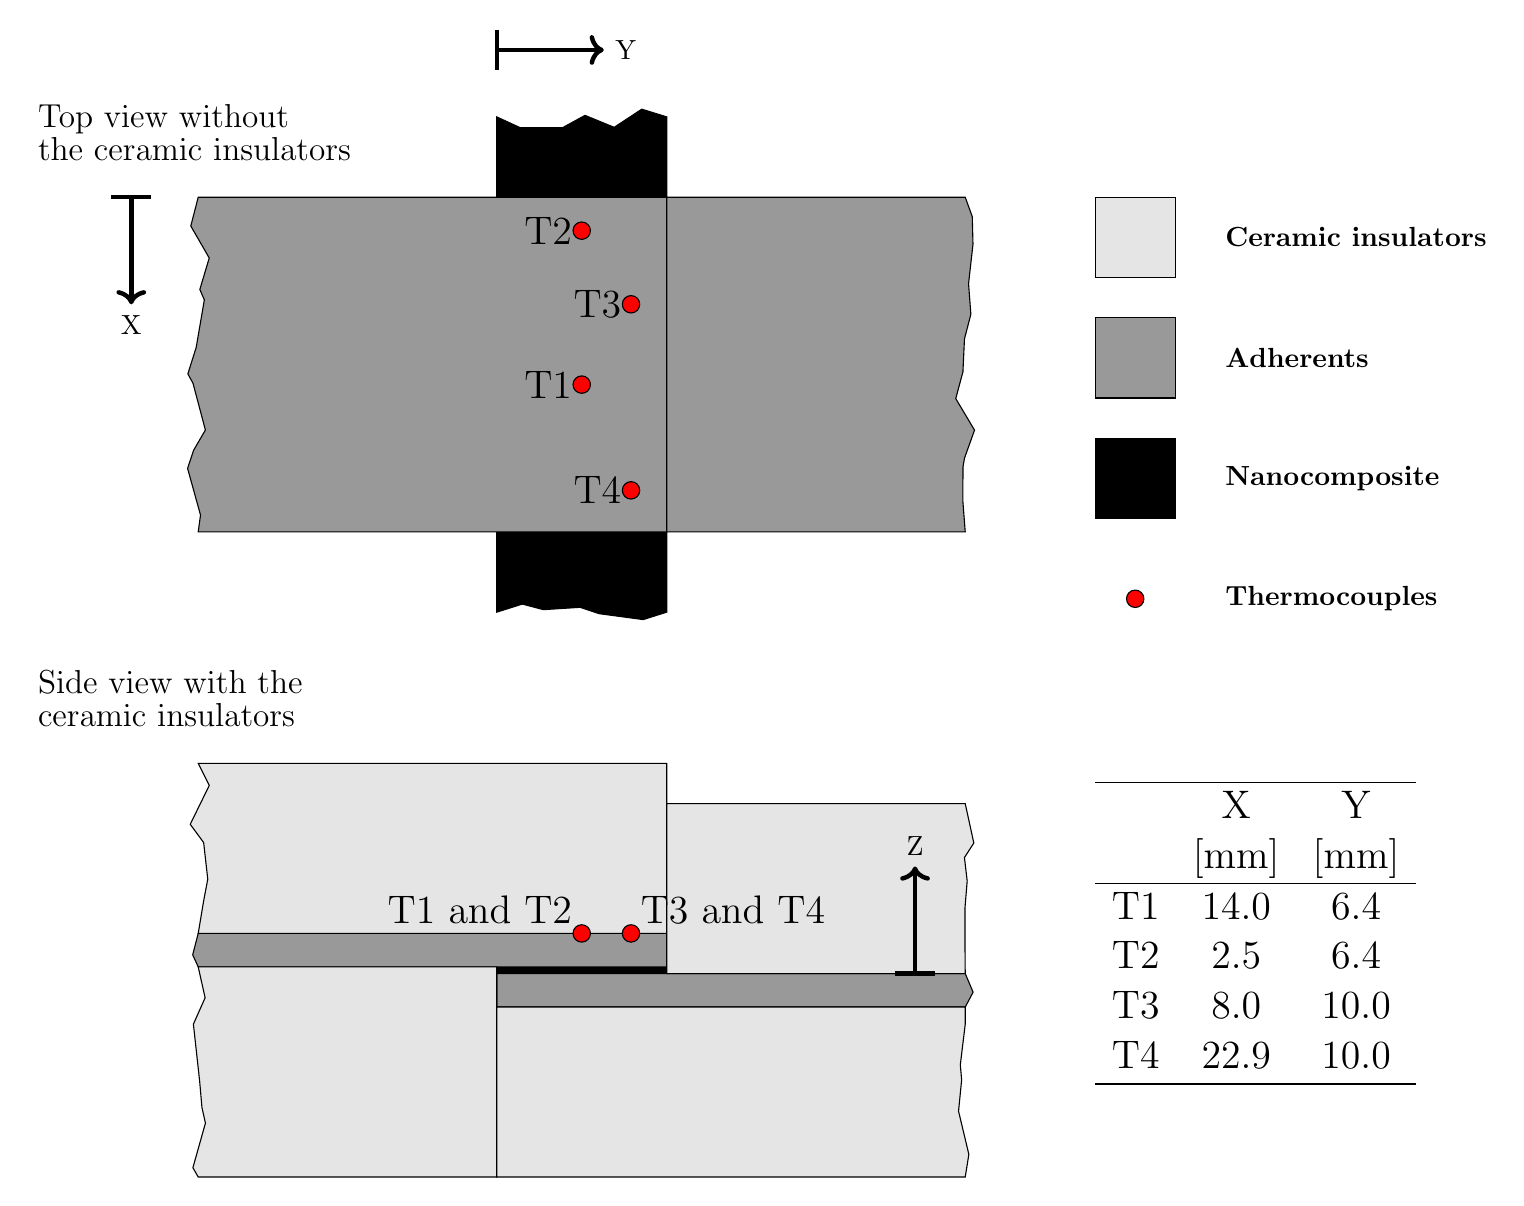
\begin{tikzpicture}[scale=0.17]

%Couleurs
\def \colceramique{black!10}
\def \colcomposite{black!40}

\def \legend{6}

%Définition des dimensions du joint soudé
\def \overlap{12.7}
\def \epceramique{12.7}
\def \epcomposite{2.5}
\def \epnanocomposite{0.5}
\def \longueur{35}
\def \gapfigure{33}
\def \largeursoudure{25}
\def \depassementsoudure{6}
\def \diacercle{0.65}

\def \gaptexte{2}

\def \llegende{8}
\def \distlegende{5}
\def \wlegendtail{3}

%%%Vue du dessus %%%
\draw (-\longueur,\gapfigure+\largeursoudure+\gaptexte) node [above right, align=left]{\large Top view without \\ \large the ceramic insulators};

%Élément chauffant
\draw[black,decoration={random steps, amplitude=4, segment length=10},fill=black] (0,\gapfigure-\depassementsoudure) decorate{-- ++(\overlap,0)} -- ++(0,2*\depassementsoudure+\largeursoudure) decorate{-- ++(-\overlap,0)} -- cycle;

%Adhérent
\draw[black,decoration={random steps, amplitude=4, segment length=10},fill=\colcomposite] 
(0,\gapfigure) -- ++(\longueur,0) decorate{-- ++(0,\largeursoudure)} -- ++(-\longueur,0) -- cycle;
\draw[black,decoration={random steps, amplitude=4, segment length=10},fill=\colcomposite] 
(\overlap,\gapfigure) -- ++(-\longueur,0) decorate{-- ++(0,\largeursoudure)} -- ++(\longueur,0) -- cycle;


%Position du thermocouple
\draw[fill=red] (0.5*\overlap,\largeursoudure+\gapfigure-14) circle (\diacercle) node [left]{\Large T1};
\draw[fill=red] (0.5*\overlap,\largeursoudure+\gapfigure-2.5) circle (\diacercle) node [left]{\Large T2};
\draw[fill=red] (0.79*\overlap,\largeursoudure+\gapfigure-8) circle (\diacercle) node [left]{\Large T3};
\draw[fill=red] (0.79*\overlap,\largeursoudure+\gapfigure-21.9) circle (\diacercle) node [left]{\Large T4};

%%% Vue du côté %%%
\draw (-\longueur,\epceramique+\epnanocomposite+\epcomposite+\gaptexte) node [above right, align=left]{\large Side view with the \\ \large ceramic insulators};

%Éléments chauffants
\draw[black,thick,fill=black] (0,0) -- ++(\overlap,0) -- ++(0,\epnanocomposite) -- ++(-\overlap,0) -- cycle;

%Adhérents
\draw[black,decoration={random steps, amplitude=4, segment length=6},fill=\colcomposite] 
(0,0) -- ++(\longueur,0) decorate{-- ++(0,-\epcomposite)} -- ++(-\longueur,0) -- cycle;
\draw[black,decoration={random steps, amplitude=4, segment length=6},fill=\colcomposite] 
(\overlap,\epnanocomposite) -- ++(-\longueur,0) decorate{-- ++(0,\epcomposite)} -- ++(\longueur,0) -- cycle;

%Céramiques
\draw[black,decoration={random steps, amplitude=4, segment length=10},fill=\colceramique] 
(0,\epnanocomposite) -- ++(-\longueur+\overlap,0) decorate{-- ++(0,-\epceramique-\epnanocomposite-\epcomposite)} -- ++(\longueur-\overlap,0) -- cycle;
\draw[black,decoration={random steps, amplitude=4, segment length=10},fill=\colceramique] 
(\overlap,\epcomposite+\epnanocomposite) -- ++(-\longueur,0) decorate{-- ++(0,\epceramique)} -- ++(\longueur,0) -- cycle;
\draw[black,decoration={random steps, amplitude=4, segment length=10},fill=\colceramique] 
(0,-\epcomposite) -- ++(\longueur,0) decorate{-- ++(0,-\epceramique)} -- ++(-\longueur,0) -- cycle;
\draw[black,decoration={random steps, amplitude=4, segment length=10},fill=\colceramique] 
(\overlap,0) -- ++(\longueur-\overlap,0) decorate{-- ++(0,\epceramique)} -- ++(-\longueur+\overlap,0) -- cycle;

%Position du thermocouple
\draw[fill=red] (0.5*\overlap,\epnanocomposite+\epcomposite) circle (\diacercle) node [above left]{\Large T1 and T2};
\draw[fill=red] (0.79*\overlap,\epnanocomposite+\epcomposite) circle (\diacercle) node [above right]{\Large T3 and T4};

% Système d'axe
\draw[ultra thick, black, ->] (0,\gapfigure+\depassementsoudure+\distlegende+\largeursoudure) -- ++(\llegende,0) node[ right] {Y}; 
\draw[ultra thick, black] (0,\gapfigure+\depassementsoudure+\distlegende+\largeursoudure+0.5*\wlegendtail) -- ++(0,-\wlegendtail); 

\draw[ultra thick, black, ->] (-\distlegende-\longueur+\overlap,\gapfigure+\largeursoudure) -- ++(0,-\llegende) node[below] {X}; 
\draw[ultra thick, black] (-\distlegende-\longueur+\overlap-0.5*\wlegendtail,\gapfigure+\largeursoudure) -- ++(\wlegendtail,0); 

\draw[ultra thick, black, ->] (\longueur-0.75*\distlegende,0) -- ++(0,\llegende) node[ above] {Z}; 
\draw[ultra thick, black] (\longueur-0.75*\distlegende-0.5*\wlegendtail,0) -- ++(\wlegendtail,0); 

%Legend
\begin{scope}[shift={(\overlap+\longueur-0.5*\legend,\gapfigure+\largeursoudure)}]
	\begin{scope}[shift={(0,0)}]
		\draw [black, fill=\colceramique] (0,0) rectangle ++(\legend,-\legend);
		\draw (1.5*\legend,-0.5*\legend) node[right]{{\textbf{Ceramic insulators}}} ;
	\end{scope}

	\begin{scope}[shift={(0,-1.5*\legend)}]
		\draw [black, fill=\colcomposite] (0,0) rectangle ++(\legend,-\legend);
		\draw (1.5*\legend,-0.5*\legend) node[right]{{\textbf{Adherents}}} ;
	\end{scope}

	\begin{scope}[shift={(0,-3*\legend)}]
		\draw [black, fill=black] (0,0) rectangle ++(\legend,-\legend);
		\draw (1.5*\legend,-0.5*\legend) node[right]{{\textbf{Nanocomposite}}} ;
	\end{scope}

	\begin{scope}[shift={(0,-4.5*\legend)}]
		\draw [fill=red] (0.5*\legend,-0.5*\legend) circle (\diacercle);
		\draw (1.5*\legend,-0.5*\legend) node[right]{{\textbf{Thermocouples}}} ;
	\end{scope}

\end{scope}

%Location of thermocouples
\begin{scope}[shift={(\overlap+\longueur+1.5*\legend,0.5*\legend)}]
	\node (thermocouple_location){ \Large
		\begin{tabular}{c c c}
			\hline
			   & X    & Y    \\
			   & [mm] & [mm] \\ \hline
			T1 & 14.0 & 6.4  \\
			T2 & 2.5  & 6.4  \\
			T3 & 8.0  & 10.0 \\
			T4 & 22.9 & 10.0 \\ \hline
		\end{tabular}
	};
\end{scope}



\end{tikzpicture}
}
	\caption{Location of thermocouples during welding experiments}
	\label{fig:2_Fig3}
\end{figure} 

\FloatBarrier
%%%%%%%%%%%%%%%%%%%%%%%%%%%%%%%%%%%%%%%%%%%%%%%%%%%%%%%%%%%%%%%%%
\section{Results and discussion}
%%%%%%%%%%%%%%%%%%%%%%%%%%%%%%%%%%%%%%%%%%%%%%%%%%%%%%%%%%%%%%%%%

%%%%%%%%%%%%%%%%%%%%%%%%%%%%%%%%%%%%%%%%%%%%%%%%%%%%%%%%%%%%%%
\subsection{Material characterization}
%%%%%%%%%%%%%%%%%%%%%%%%%%%%%%%%%%%%%%%%%%%%%%%%%%%%%%%%%%%%%%

The $C_p$ obtained by MDSC are presented at Table \ref{tab:T2_table1}. 
The thermal conductivity as a function of temperature for CF/PEEK, the PEI/MWCNT nanocomposite and the alumina silicate are reported in Table \ref{tab:T2_table2}. 
The asperities roughness $\sigma_{asp}$ and asperities average slopes $m_{asp}$ were measured respectively at \mbox{0.26\,$\mu$m} and 0.15. 
The microhardness was set at \mbox{0.1\,GPa} in the model. 

\begin{table}[ht]
	\centering
	\caption{Results for Specific heat measurements}
	\begin{tabular}{@{}cccc@{}}
		\toprule
		   Temperature    &           CF/PEEK            &          PEI/MWCNT           &       Alumina Silicate       \\
		{[}$^{\circ}$C{]} & {[}J\,kg$^{-1}$\,K$^{-1}${]} & {[}J\,kg$^{-1}$\,K$^{-1}${]} & {[}J\,kg$^{-1}$\,K$^{-1}${]} \\ \midrule
		       40         &             926              &             1059             &                              \\
		       97         &                              &                              &             975              \\
		       139        &             1265             &                              &                              \\
		       159        &             1359             &                              &                              \\
		       207        &                              &             1561             &                              \\
		       227        &                              &             1765             &                              \\
		       310        &             1809             &                              &                              \\
		       343        &             2400             &                              &                              \\
		       360        &             1792             &                              &                              \\
		       399        &             1790             &             1955             &                              \\ \bottomrule
	\end{tabular}
	\label{tab:T2_table1}
\end{table}

\begin{table}[ht]
	\centering
	\caption{Results for thermal conductivity measurement}
	\begin{tabular}{@{}ccccc@{}}
		\toprule
		   Temperature    &           CF/PEEK           &           CF/PEEK           &          PEI/MWCNT          &      Alumina Silicate       \\
		                  &          Parallel           &        Perpendicular        &                             &                             \\
		{[}$^{\circ}$C{]} & {[}W\,m$^{-1}$\,K$^{-1}${]} & {[}W\,m$^{-1}$\,K$^{-1}${]} & {[}W\,m$^{-1}$\,K$^{-1}${]} & {[}W\,m$^{-1}$\,K$^{-1}${]} \\ \midrule
		       20         &            2.25             &            0.55             &            0.41             &                             \\
		       40         &                             &                             &            0.43             &             5.7             \\
		       60         &                             &                             &            0.43             &                             \\
		       110        &                             &                             &            0.46             &                             \\
		       150        &                             &                             &            0.48             &                             \\
		       200        &            3.02             &            0.73             &                             &                             \\ \bottomrule
	\end{tabular}
	\label{tab:T2_table2}
\end{table}

\FloatBarrier
%%%%%%%%%%%%%%%%%%%%%%%%%%%%%%%%%%%%%%%%%%%%%%%%%%%%%%%%%%%%%%
\subsection{Modelling results}
%%%%%%%%%%%%%%%%%%%%%%%%%%%%%%%%%%%%%%%%%%%%%%%%%%%%%%%%%%%%%%

The model was first validated with experimental data. 
Four resistance welding experiments under different conditions served as references. 
The same welding conditions were reproduced by the model and the resulting validation curves are presented in \mbox{Fig. \ref{fig:2_Fig4}}. 
Initial modelling efforts neglected the electrical contact resistance between the electrodes and the nanocomposite and did not fit the observations. 
Upon further inspection, the contact electrical resistance was measured by subtracting the theoretical nanocomposite’s HE electrical resistance to the total resistance of the welding setup between both electrodes measured with a handheld multimeter. 
The electrical contact resistance accounts for approximately 50\% of the total electrical resistance of the setup. 
Reducing the power by 45\% provided a good agreement with the experiments allowing for the model to explore the general behaviour of the welding process. 

\begin{figure}[ht]
	\center
	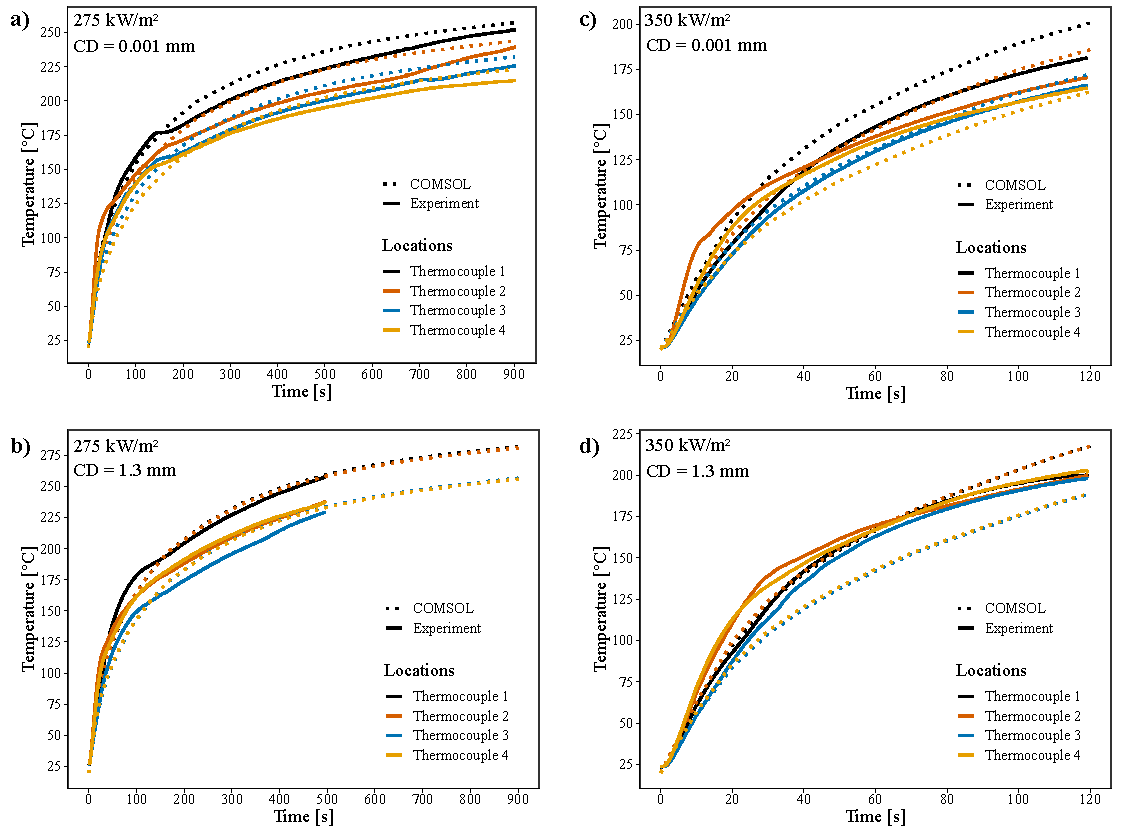
\includegraphics[width=0.95\textwidth]{2_Fig4}
	\caption{Validation curves for the model under various welding conditions with solid line representing experimental results, dotted lines for COMSOL results and colours assigned to each thermocouple locations \cite{Brassard2019b}}
	\label{fig:2_Fig4}
\end{figure} 

\FloatBarrier
As it was not possible to monitor the temperature directly at the weld interface without disturbing the thermal profile and affecting the results, the model offers us insight that could not be obtained from experiments. 
The temperature distribution along the length of the weld (\textit{x-axis}) varies based on the clamping distance and power density, as previously reported \cite{Talbot2013} (\mbox{Fig. \ref{fig:2_Fig5}}). 
It can be controlled with a variation of the clamping distance but the profile across the width of the weld (\textit{y-axis}) is mostly unaffected by the clamping distance. 
A cold edge (at y = \mbox{0\,mm} in \mbox{Fig. \ref{fig:2_Fig5}}) is always present at the top surface of the nanocomposite on the side where the adherent exits the weld due edge effects caused by the high axial thermal conductivity of the carbon fibres in the UD TPC adherents. 
On the bottom surface of the nanocomposite, the cold edge is located on the mirror side of the weld (at y = \mbox{12.7\,mm}) due to the adherent leaving the weld on the other side (details in bottom sections of \mbox{Fig. \ref{fig:2_Fig2}} and \mbox{Fig. \ref{fig:2_Fig3}}). 

\begin{figure}[ht]
	\center
	\includegraphics[width=\textwidth]{2_Fig5}
	\caption{Temperature distributions after 900 and 120 seconds for respective power densities of 275 and \SI{350}{\kilo\watt\per\square\metre} at the interface on top of the nanocomposite HE with clamping distances of 0.001, 1.3 and 2.0 mm \cite{Brassard2019b}}
	\label{fig:2_Fig5}
\end{figure} 

\FloatBarrier
Simulations were performed to observe the temperature uniformity along the length of the weld (\textit{x-axis}) to optimize the clamping distance and to evaluate the sensitivity of this parameter. 
The optimal clamping distance is the distance which minimizes the temperature difference between the centre of the weld and the maximum temperature at the edges. 
Polymer degradation at the edge begins when the clamping distance is too large. 
The clamping distances for both conditions vary almost linearly as a function of the power density over the experimental domain (\mbox{Fig. \ref{fig:2_Fig6}}). 
Additionally, an almost constant difference of \mbox{0.4\,mm} exists between the optimal clamping distance and the length causing thermal degradation at the edge. 
Thus, the dimensional tolerance for the location of the electrodes during the resistance welding with a nanocomposite HE process can be on the order of a few tenths of millimetres. 

\begin{figure}[ht]
	\center
	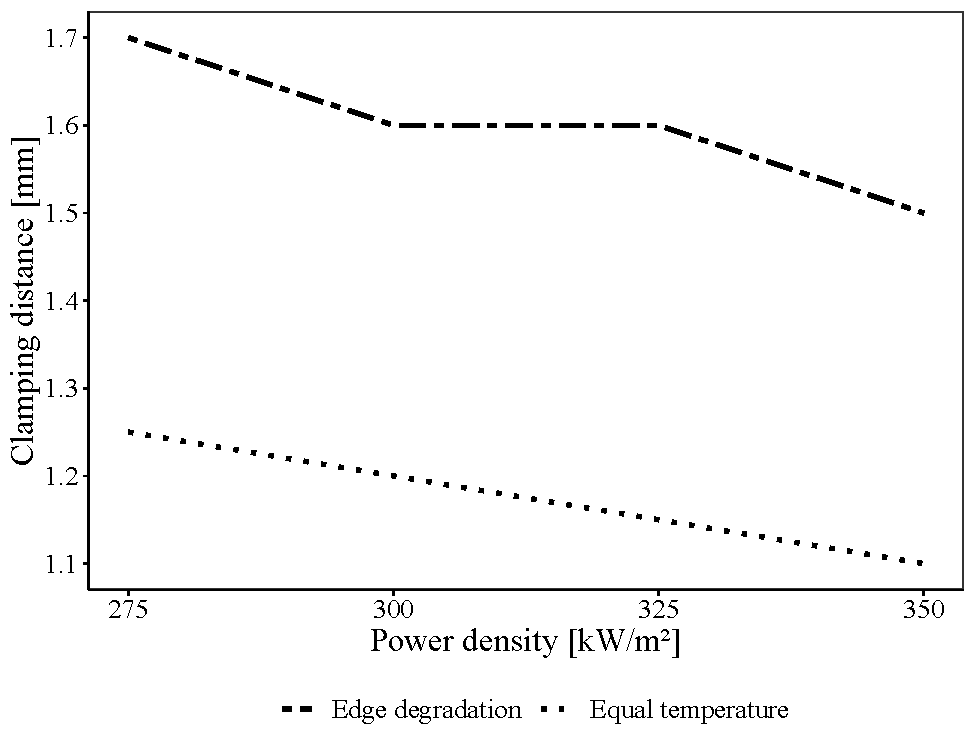
\includegraphics[scale=0.75]{2_Fig6}
	\caption{Sensitivity analysis for the clamping distance showing the clamping distances resulting in optimal temperature distribution and the beginning of edge degradation as a function of power density \cite{Brassard2019b}}
	\label{fig:2_Fig6}
\end{figure} 

It is now possible to expand the scope of the analysis. 
The resulting process window (\mbox{Fig. \ref{fig:2_Fig7}}) presents the time required for the hottest point at the interface to reach \mbox{370\,$^{\circ}$C}, \mbox{400\,$^{\circ}$C} and \mbox{440\,$^{\circ}$C}, \mbox{10\,$^{\circ}$C} below the degradation temperature of PEI \cite{Carroccio2000}. 
The temperature of the lower bound and the average temperature within the weld at that moment (approximately \mbox{390\,$^{\circ}$C}) are higher than the reported temperatures required to obtain reptation times compatible with the resistance welding process for PEI/PEEK interfaces \cite{Bastien1991}. 
On the other hand, the addition of a large fraction of MWCNT is limiting polymer chain mobility at lower temperatures \cite{Mu2009,Kabanemi2010} and a higher temperature or more time is required to achieve similar diffusion of the chains. 
Additional welding experiments were conducted based on the suggested processing window and previous results to validate the model’s results. 
The average single lap shear strength for all welded joints are presented in \mbox{Fig. \ref{fig:2_Fig7}}.  

\begin{figure}[ht]
	\center
	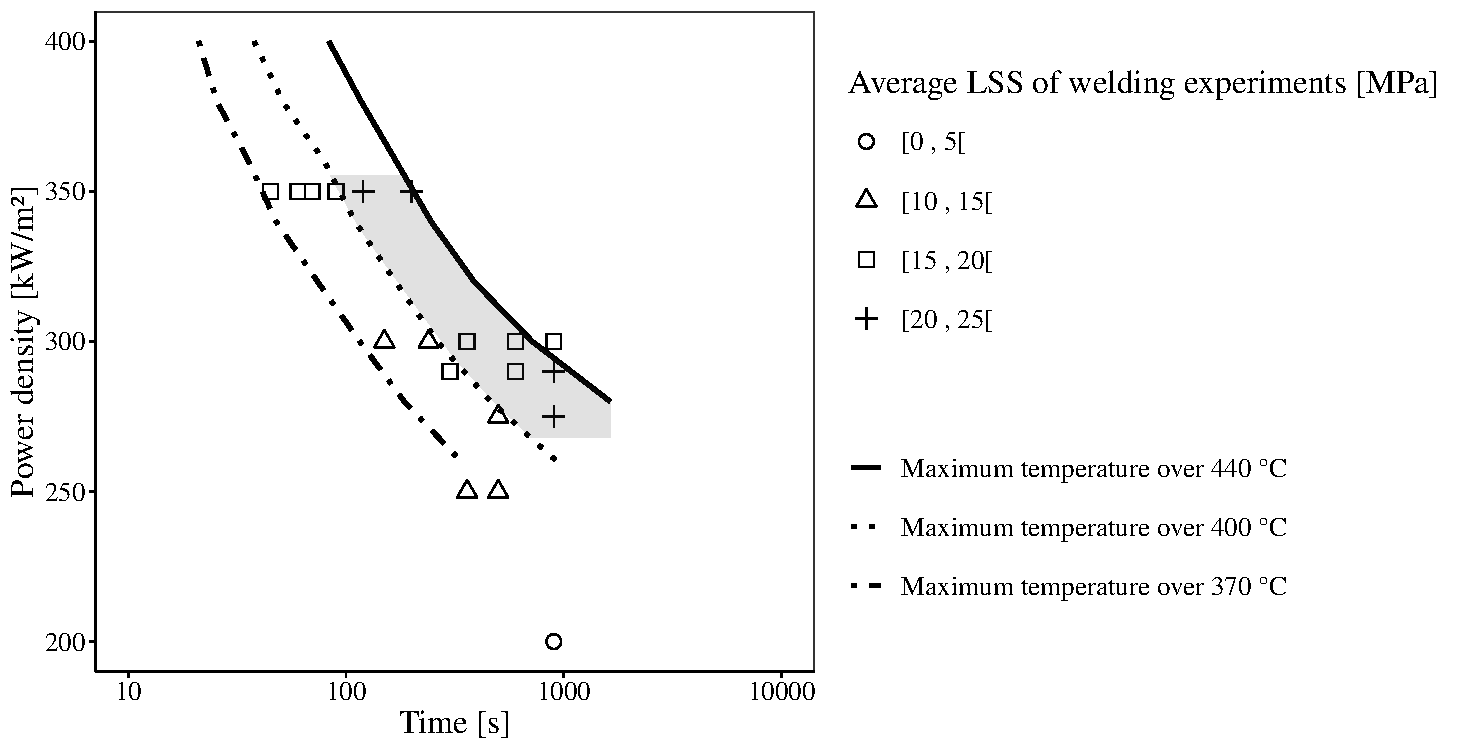
\includegraphics[width=\textwidth]{2_Fig7}
	\caption{Process window (grayed zone) based on the simulation results with optimal clamping distance, the lines represent the time to reach a local maximum temperatures of 370\,$^{\circ}$C, 400\,$^{\circ}$C and 440\,$^{\circ}$C on the top surface of the nanocomposite in the model while the markers presents the single lap shear results from all the welding experiments \cite{Brassard2019b}}
	\label{fig:2_Fig7}
\end{figure} 

\FloatBarrier
%%%%%%%%%%%%%%%%%%%%%%%%%%%%%%%%%%%%%%%%%%%%%%%%%%%%%%%%%%%%%%
\subsection{Welding experiments}
%%%%%%%%%%%%%%%%%%%%%%%%%%%%%%%%%%%%%%%%%%%%%%%%%%%%%%%%%%%%%%

Current leakage in the composite adherents can be a problem for resistance welding of carbon fibre laminates at high power and it currently limits resistance welding with a nanocomposite HE to unidirectional adherents. 
The model pointed toward the possibility to produce welds at lower power and longer times to reduce the voltage difference along the length of the nanocomposite HE to minimize the risk of current leakage. 
Successful welding tests were performed with power densities as low as \mbox{250\,kW\,m$^{-2}$} (resulting LSS $\sim$ \mbox{14\,MPa}). 
These additional tests, along with previous results are included in \mbox{Fig. \ref{fig:2_Fig7}} and in \mbox{Table \ref{tab:T2_table3} and \ref{tab:T2_table4}}. 
The highest average LSS (\mbox{24.9\,MPa}) was obtained at a power density of \mbox{350\,kW\,m$^{-2}$}, a clamping distance of \mbox{1.3\,mm}, a pressure of \mbox{1\,MPa} on the weld and a welding time of \mbox{120\,s}. 
This LSS corresponds to a 28\% improvement relative to previously published results, thanks to a better processing window predicted by the finite element model, with LSS ranging from 14.1 to \mbox{35.2\,MPa}. 
LSS results of joints welded using non-optimal sets of welding parameters are also presented in Table \ref{tab:T2_table3} and \ref{tab:T2_table4} \cite{Brassard2019b}. 
A welding experiment at \mbox{200\,kW\,m$^{-2}$} during \mbox{900\,s} did not result in a successful weld.  

\begin{table}[htb]
	\centering
	\caption{LSS tests results}
	\resizebox{0.98\textwidth}{!}{
		\begin{tabular}{@{}lll L{1.6cm} l C{1.1cm} C{1.1cm} C{1.1cm} C{1.1cm} C{1.1cm} C{1.1cm} C{1.1cm} @{}}
		\toprule
		Power              & Clamping & Pressure  & Values            &       &                                                         \multicolumn{7}{c}{Time}                                                          \\
		density            & distance &           &                   &       &                                                        \multicolumn{7}{c}{{[}s{]}}                                                        \\
		{[}kW\,m$^{-2}${]} & {[}mm{]} & {[}MPa{]} &                   &       & 45                & 60                & 70                & 90                & 120               & 150               & 200               \\ midrule
		300                & 1.2      & 1.0       & LSS \mbox{± S.D.} & [MPa] &                   &                   &                   &                   &                   & 14.9 \mbox{± 5.6} &                   \\
		                   &          &           & Samples           &       &                   &                   &                   &                   &                   & 3                 &                   \\
		350                & 0        & 1.0       & LSS \mbox{± S.D.} & [MPa] &                   &                   &                   &                   & 15.2 \mbox{± 1.7} &                   &                   \\
		                   &          &           & Samples           &       &                   &                   &                   &                   & 4                 &                   &                   \\
		                   & 1.0      & 1.0       & LSS \mbox{± S.D.} & [MPa] &                   &                   &                   &                   & 13.0 \mbox{± 4.4} &                   &                   \\
		                   &          &           & Samples           &       &                   &                   &                   &                   & 3                 &                   &                   \\
		                   & 1.1      & 1.0       & LSS \mbox{± S.D.} & [MPa] & 17.4 \mbox{± 3.6} &                   &                   &                   &                   &                   & 21.0 \mbox{± 5.6} \\
		                   &          &           & Samples           &       & 3                 &                   &                   &                   &                   &                   & 3                 \\
		                   & 1.3      & 1.0       & LSS \mbox{± S.D.} & [MPa] &                   &                   &                   &                   & 24.9 \mbox{± 9.7} &                   &                   \\
		                   &          &           & Samples           &       &                   &                   &                   &                   & 4                 &                   &                   \\
		                   & 1.5      & 1.0       & LSS \mbox{± S.D.} & [MPa] &                   & 16.4 \mbox{± 7.8} & 18.6 \mbox{± 2.0} & 15.5 \mbox{± 3.8} & 19.6 \mbox{± 3.5} &                   &                   \\
		                   &          &           & Samples           &       &                   & 3                 & 3                 & 3                 & 3                 &                   &                   \\ \bottomrule
		\end{tabular}}
	\label{tab:T2_table3}
\end{table}

\begin{table}[htb]
	\centering
	\caption{LSS tests results (continued)}
	\resizebox{0.98\textwidth}{!}{
		\begin{tabular}{@{}lll L{1.6cm} l C{1.1cm} C{1.1cm} C{1.1cm} C{1.1cm} C{1.1cm} C{1.1cm}@{}}
			\toprule
			Power              & Clamping & Pressure  & Values            &           &                                             \multicolumn{6}{c}{Time}                                               \\
			density            & distance &           &                   &           &                                             \multicolumn{6}{c}{{[}s{]}}                                              \\
			{[}kW\,m$^{-2}${]} & {[}mm{]} & {[}MPa{]} &                   &           & 240               & 300               & 360               & 500              & 600               & 900               \\ \midrule
			200                & 0        & 1.0       & LSS \mbox{± S.D.} & {[}MPa{]} &                   &                   &                   &                  &                   & 3.1 \mbox{± NA}   \\
			                   &          &           & Samples           &           &                   &                   &                   &                  &                   & 1                 \\
			250                & 0        & 1.0       & LSS \mbox{± S.D.} & {[}MPa{]} & 13.2 \mbox{± NA}  &                   & 14.1 \mbox{± NA}  &                  &                   &                   \\
			                   &          &           & Samples           &           & 1                 &                   & 1                 &                  &                   &                   \\
			275                & 0        & 1.0       & LSS \mbox{± S.D.} & {[}MPa{]} &                   &                   &                   &                  &                   & 20.0 \mbox{± 2.7} \\
			                   &          &           & Samples           &           &                   &                   &                   &                  &                   & 4                 \\
			                   & 1.3      & 1.0       & LSS \mbox{± S.D.} & {[}MPa{]} &                   &                   &                   & 24.3 \mbox{± NA} &                   &                   \\
			                   &          &           & Samples           &           &                   &                   &                   & 1                &                   &                   \\
			290                & 0        & 1.0       & LSS \mbox{± S.D.} & {[}MPa{]} &                   &                   &                   &                  &                   & 17.8 \mbox{± 2.2} \\
			                   &          &           & Samples           &           &                   &                   &                   &                  &                   & 4                 \\
			                   &          & 1.4       & LSS \mbox{± S.D.} & {[}MPa{]} &                   &                   &                   &                  &                   & 21.4 \mbox{± 2.7} \\
			                   &          &           & Samples           &           &                   &                   &                   &                  &                   & 2                 \\
			                   & 1.2      & 1.0       & LSS \mbox{± S.D.} & {[}MPa{]} &                   & 18.9 \mbox{± 7.0} &                   &                  & 17.7 \mbox{± 4.3} &                   \\
			                   &          &           & Samples           &           &                   & 3                 &                   &                  & 3                 &                   \\
			300                & 0        & 1.0       & LSS \mbox{± S.D.} & {[}MPa{]} & 13.8 \mbox{± 3.8} &                   & 17.7 \mbox{± 1.1} &                  &                   & 16.5 \mbox{± 0.7} \\
			                   &          &           & Samples           &           & 3                 &                   & 3                 &                  &                   & 3                 \\
			                   & 1.2      & 1.0       & LSS \mbox{± S.D.} & {[}MPa{]} &                   &                   &                   &                  & 19.4 \mbox{± 3.0} &                   \\
			                   &          &           & Samples           &           &                   &                   &                   &                  & 3                 &                   \\ \bottomrule
		\end{tabular}}
	\label{tab:T2_table4}
\end{table}

\FloatBarrier
%%%%%%%%%%%%%%%%%%%%%%%%%%%%%%%%%%%%%%%%%%%%%%%%%%%%%%%%%%%%%%
\subsection{Nanocomposite tensile strength}
%%%%%%%%%%%%%%%%%%%%%%%%%%%%%%%%%%%%%%%%%%%%%%%%%%%%%%%%%%%%%%

Due to the high loading of MWCNTs in the nanocomposite, it is expected that its ductility and tensile strength are impacted. 
Average tensile strength of 72.2 $\pm$ \mbox{19.4\,MPa} and elongation at break of 5.2 $\pm$ 1.7\% were obtained from tensile tests on nanocomposite samples. 
During these tests, all samples had brittle failure mode without a ductile plateau. 
This can be contrasted to virgin properties of ULTEM 1010 (tensile strength of 110 MPa and 60\% elongation) to show that the mechanical behaviour of the nanocomposite is severely affected by the 10\% wt. loading of MWCNTs, which was also noticeable during the handling of the HE. 
The variability in the performances of the nanocomposite is in line with the variability observed in the LSS tests. 

%%%%%%%%%%%%%%%%%%%%%%%%%%%%%%%%%%%%%%%%%%%%%%%%%%%%%%%%%%%%%%
\subsection{Fractography}
%%%%%%%%%%%%%%%%%%%%%%%%%%%%%%%%%%%%%%%%%%%%%%%%%%%%%%%%%%%%%%

Direct imaging of the fractured surfaces (\mbox{Fig. \ref{fig:2_Fig8}}) provided some insight on the failure modes of the welded joints. 
First, signs of unstable crack propagation due to the brittleness of the nanocomposite are clearly visible. 
Evenly spaced cracks in the matrix residues are visible on one face (\mbox{Fig. \ref{fig:2_Fig8}}a) and evenly spaced ridges are visible in the mirror matching face (\mbox{Fig. \ref{fig:2_Fig8}}b). 
A close look at those ridges (\mbox{Fig. \ref{fig:2_Fig8}}c) shows polymer well bonded to the composite substrate. 
Second, broken fibres can be seen embedded on top of nanocomposite residues still attached to opposing faces (\mbox{Fig. \ref{fig:2_Fig8}}d). 
Both of these observations are signs that the bonding between the nanocomposite and the composite adherents is not the weakest link. 
Signs of thermal degradation could be observed in \mbox{Fig. \ref{fig:2_Fig8}}e serving as an example of porosities left by vaporized polymer. 
Carbon fibres with no polymer attached to them or degraded polymer residues can be seen at other locations. 
Finally, when thermal degradation and unstable cracks combine in the same zone, a different failure mode can be observed where cracks form between adjacent porosities and through the nanocomposite (\mbox{Fig. \ref{fig:2_Fig8}}f).

\begin{figure}[htb]
	\center
	\includegraphics[width=0.98\textwidth]{2_Fig8}
	\caption{SEM fractography of welded specimens showing : a) unstable crack propagation causing evenly spaced cracks in the nanocomposite, b) and c) ridges left on the opposing surface when cracks forms, d) fibre adherence to the nanocomposite HE, e) signs of localized thermal degradation, f) unstable crack propagation combined with thermal degradation \cite{Brassard2019b}}
	\label{fig:2_Fig8}
\end{figure} 

The SEM observations, reduced tensile strength and low elongation at break of the nanocomposite combine to infer that the current limiting factor for resistance welding of thermoplastic composites with a nanocomposite HE is the nature of the nanocomposite itself. 
In traditional resistance welding, a compliant resin rich layer is present between the adherents and can dissipate energy through plastic deformation. 
With the current brittle nanocomposite, as soon as cracking occurs, cracks will propagate in an unstable fashion through the interface. 
Improvements to the process could come either by combining the brittle nanocomposite with an underlying compliant layer of material to produce a flexible joint or by modifying the composition of the nanocomposite to increase its ductility while maintaining its electrical conductivity. 

\FloatBarrier
%%%%%%%%%%%%%%%%%%%%%%%%%%%%%%%%%%%%%%%%%%%%%%%%%%%%%%%%%%%%%%%%%
\section{Conclusion}
%%%%%%%%%%%%%%%%%%%%%%%%%%%%%%%%%%%%%%%%%%%%%%%%%%%%%%%%%%%%%%%%%

This work presented the development of a finite element model for the resistance welding of thermoplastic composites, using a nanocomposite heating element. 
The model allowed to establish a processing window leading to an improvement of up to 28\% in the LSS of welded joints. 
Furthermore, the model and new experiments presented here increased our knowledge of the phenomena at play when welding using these newly developed HE. 
The model demonstrated the possibility to produce welds at lower power densities and this was validated experimentally. 
Finally, mechanical testing and fractography analysis of the nanocomposite HE highlighted its brittle nature which is currently the limiting factor in the mechanical strength of the welded joints. 
Future work will aim at producing a conductive nanocomposite with a higher ductility than the current solution or to bond the nanocomposite to a compliant intermediary layer. 

%%%%%%%%%%%%%%%%%%%%%%%%%%%%%%%%%%%%%%%%%%%%%%%%%%%%%%%%%%%%%%%%%
\section{Acknowledgements}
%%%%%%%%%%%%%%%%%%%%%%%%%%%%%%%%%%%%%%%%%%%%%%%%%%%%%%%%%%%%%%%%%

This work was supported by ArianeGroup and CREPEC. 
The authors would also like to thank Vincent Rohart for his time and help for the SEM imaging and Prof. Philippe Pasquier for the thermal conductivity measurements. 

%%%%%%%%%%%%%%%%%%%%%%%%%%%%%%%%%%%%%%%%%%%%%%%%%%%%%%%%%%%%%%%%%
\section{Supplementary Information}
%%%%%%%%%%%%%%%%%%%%%%%%%%%%%%%%%%%%%%%%%%%%%%%%%%%%%%%%%%%%%%%%%

This section presents a summary of all the materials properties used in the model. 

The relative permittivity for the PEI/MWCNT nanocomposite was calculated with the law of mixture from the reported value of 3.15 for SABIC’s PEI grade ULTEM 1010 and a relative permittivity of 15 for MWCNTs \cite{Katsounaros2011}. 

% Please add the following required packages to your document preamble:
% \usepackage{booktabs}
\begin{table}[ht]
	\centering
	\caption{List of all specific heat used in the model}
	\resizebox{\textwidth}{!}{
		\begin{tabular}{@{}cccccc@{}}
			\toprule
			Temperature & CF/PEEK    & PEI/MWCNT  & Alumina Silicate & Copper     & GPO3       \\
			{[}$^{\circ}$C{]} & {[}J\,kg$^{-1}$\,K$^{-1}${]} & {[}J\,kg$^{-1}$\,K$^{-1}${]} & {[}J\,kg$^{-1}$\,K$^{-1}${]}  & {[}J\,kg$^{-1}$\,K$^{-1}${]} & {[}J\,kg$^{-1}$\,K$^{-1}${]} \\ \midrule
			
			Constant    &            &            &                  & 385        & 1260       \\
			40          & 926        & 1059       &                  &            &            \\
			97          &            &            & 975              &            &            \\
			139         & 1265       &            &                  &            &            \\
			159         & 1359       &            &                  &            &            \\
			207         &            & 1561       &                  &            &            \\
			227         &            & 1765       &                  &            &            \\
			310         & 1809       &            &                  &            &            \\
			343         & 2400       &            &                  &            &            \\
			360         & 1792       &            &                  &            &            \\
			399         & 1790       & 1955       &                  &            &            \\ \midrule
			Source      & Measured   & Measured   & Measured         & COMSOL     & Suppliers  \\ \bottomrule
	\end{tabular} }
	\label{tab:SI2_table1}
\end{table}

\begin{table}[ht]
	\centering
	\caption{List of all thermal conductivity used in the model}
	\resizebox{\textwidth}{!}{%
		\begin{tabular}{@{}ccccccc@{}}
			\toprule
			Temperature & CF/PEEK   & CF/PEEK       & PEI/MWCNT & Alumina   & Copper    & GPO3      \\
			& Parallel  & Perpendicular &           & Silicate  &           &           \\
			{[}$^{\circ}$C{]} & {[}W\,m$^{-1}$\,K$^{-1}${]} & {[}W\,m$^{-1}$\,K$^{-1}${]} & {[}W\,m$^{-1}$\,K$^{-1}${]} & {[}W\,m$^{-1}$\,K$^{-1}${]} & {[}W\,m$^{-1}$\,K$^{-1}${]} & {[}W\,m$^{-1}$\,K$^{-1}${]} \\ \midrule
			Constant    &           &               &           & 5.7       & 400       & 0.27      \\
			20          & 2.25      & 0.55          & 0.41      &           &           &           \\
			40          &           &               & 0.30      &           &           &           \\
			60          &           &               & 0.43      &           &           &           \\
			110         &           &               & 0.46      &           &           &           \\
			150         &           &               & 0.48      &           &           &           \\
			200         & 3.02      & 0.73          &           &           &           &           \\ \midrule
			Source      & Measured  & Measured      & Measured  & Measured  & COMSOL    & Suppliers \\ \bottomrule
		\end{tabular}%
	}
	\label{tab:SI2_table2}
\end{table}

% Please add the following required packages to your document preamble:
% \usepackage{booktabs}
% \usepackage{graphicx}
\begin{table}[ht]
	\centering
	\caption{List of all densities used in the model}
	\resizebox{\textwidth}{!}{%
		\begin{tabular}{@{}llllll@{}}
			\toprule
			Temperature       & CF/PEEK            & PEI/MWCNT          & Alumina Silicate   & Copper             & GPO3               \\
			{[}$^{\circ}$C{]} & {[}kg\,m$^{-3}${]} & {[}kg\,m$^{-3}${]} & {[}kg\,m$^{-3}${]} & {[}kg\,m$^{-3}${]} & {[}kg\,m$^{-3}${]} \\ \midrule
			Constant          &                    & 1320               & 2500               & 8700               & 1800               \\
			0                 & 1601               &                    &                    &                    &                    \\
			50                & 1598               &                    &                    &                    &                    \\
			100               & 1593               &                    &                    &                    &                    \\
			150               & 1586               &                    &                    &                    &                    \\
			200               & 1575               &                    &                    &                    &                    \\
			250               & 1563               &                    &                    &                    &                    \\
			300               & 1551               &                    &                    &                    &                    \\
			350               & 1537               &                    &                    &                    &                    \\
			400               & 1524               &                    &                    &                    &                    \\ \midrule
			Source            & \cite{Talbot2013}  & Measured           & Measured           & COMSOL             & Suppliers          \\ \bottomrule
		\end{tabular}%
	}
	\label{tab:SI2_table3}
\end{table}

\begin{table}[ht]
	\centering
	\caption{List of electrical properties for the model}
	\begin{tabular}{@{}lccccc@{}}
		\toprule
		&                   & \multicolumn{2}{c}{PEI/MWCNT} & \multicolumn{2}{c}{Copper}  \\ \midrule
		Electrical conductivity & {[}S\,m$^{-1}${]} & 80         & Measured         & $5.998 \times 10^7$ & COMSOL \\
		Relative permittivity   & {[} \ {]}         & 4.3        & Calculated       & 1                  & COMSOL \\ \bottomrule
	\end{tabular}%
	\label{tab:SI2_table4}
\end{table}

\FloatBarrier             % Second thème (Doctorat) ou "Résultats théoriques et expérimentaux" (Maîtrise).
\selectlanguage{french}
\Chapter{SOUDAGE D'UNE JONCTION FLEXIBLE}\label{sec:Theme3}

Ce chapitre présente les travaux menés afin de produire une jonction flexible rencontrant les requis du cahier des charges d'ArianeGroup. 
La planification des travaux, la réalisation des expériences et l'analyse des résultats ont été menées par David Brassard sous la supervision de Jason R. Tavares et Martine Dubé. 
Adrien Métafiot, durant son doctorat, a effectué la sélection des deux premiers élastomères ainsi que leur caractérisation thermique. 

\section{Étendue du problème}

Les deux précédents chapitres de cette thèse se concentraient sur la réalisation d'une soudure entre un élément chauffant nanocomposite et un composite à matrice thermoplastique \mbox{(Fig. \ref{fig:scema_double_jonction})}. 
Cette partie du joint soudé constitue uniquement la moitié du joint structurel qui vise à être produit dans le cadre de ce projet. 
Pour terminer le joint, une seconde soudure, cette fois entre l'élément chauffant nanocomposite et un élastomère thermoplastique, doit être produite. 
Une fois la jonction obtenue, il est nécessaire d'en évaluer les performances afin de les comparer aux valeurs du cahier des charges d'ArianeGroup. 

\begin{figure}[h]
	\centering
	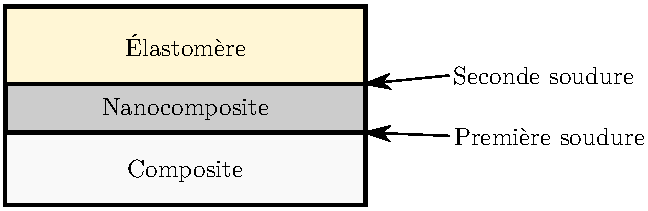
\includegraphics[scale=1]{jonction_multi_materiau.pdf}
	\caption{Schéma de la soudure multimatériaux présentant les deux soudures}
	\label{fig:scema_double_jonction}
\end{figure}

Aucun exemple d'un tel type de soudure similaire n'a pu être répertorié lors de la revue de la littérature. 
Ainsi, en raison de la nature exploratoire de cette portion du projet, les travaux de caractérisation sont réalisés avec une approche progressive et méthodique. 

\section{Méthodologie}

La première caractéristique à valider avant de penser au soudage est la stabilité thermique de l'élastomère. 
Il est nécessaire de vérifier que ce dernier pourra résister aux températures rencontrées lors du soudage sans se dégrader. 
Par la suite, des essais de caractérisation mécanique viennent valider les propriétés mécaniques de l'élastomère.
Ce dernier devant en effet rencontrer les requis du cahier des charges. 
En parallèle à la caractérisation mécanique, des essais progressifs de soudage sont mis en œuvre pour valider la possibilité de souder le matériau choisi. 

\subsection{Matériaux}

L'élastomères retenus était un copolymère multibloc (Fig. \ref{fig:polymere_multi_bloc}) de PEI et de polysiloxane  produit par SABIC sous le nom commercial ULTEM STM1500 avec des segments successifs de longueur variables  \cite{mark2013,Holden2002}. 
Il est à noter que la nature exacte de la structure du PEI-siloxane est matière à caution puisqu'un autre chercheur présente la structure comme un simple copolymère alterné (Fig. \ref{fig:polymere_alternee}) \cite{Hatui2015}. 
Toujours selon ce dernier auteur, le PEI-siloxane serait miscible avec le PEI. 

Les éléments chauffants ainsi que les adhérents en composite ont la même composition et ont été produits selon la même méthode que dans les chapitres \ref{sec:Theme1} et \ref{sec:Theme2}. 

\subsection{Caractérisation de la stabilité thermique des élastomères et du nanocomposite}

Des analyses thermogravimétriques (TGA) de l'élastomère ont été réalisées avec un appareil TA Instruments Q500. 
Tel que présenté dans la norme ASTM E2550 - 17, les échantillons ont été soumis à une rampe de \SI[locale=FR]{10}{\celsius\per\minute} jusqu'à une température de \SI[locale=FR]{800}{\celsius} sous une atmosphère régulière. 

Une seconde méthode plus sensible a été employée pour évaluer la stabilité thermique de l'élastomère. 
Les essais de TGA permet de détecter la présence de dégradation lorsque la masse de l'échantillon change. 
Cependant, lorsque la dégradation se produit par une modification de la structure du polymère, par scission de chaînes ou par réaction entre celles-ci, une mesure de la masse peut être insensible à ce changement. 
Ainsi, une mesure indirecte de la viscosité durant un brassage à haute température a pu être réalisée pour certains matériaux en mesurant l'évolution temporelle du couple lors de la production d'un mélange en condition isotherme à l'aide d'un mélangeur interne Haake PolyLab OS. 
Cette mesure ne pourra pas mesurer le degré de dégradation de l'élastomère mais elle permettra d'identifier la présence et l'évolution d'un mécanisme de dégradation. 
Une méthode permettant de quantifier la dégradation serait de mesurer l'évolution de la masse moléculaire ($M_n$ et $M_w$) du polymère avant le mélange et à divers moments du mélange. 

\subsection{Caractérisation mécanique des élastomères}

Les propriétés mécaniques des élastomères sont validées à l'aide d'essais de traction. 
Les essais de traction ont été effectués avec un échantillon de type V selon la norme ASTM~D638-14. 
Une plaque de \SI[locale=FR]{3.2}{\milli\metre} d'épaisseur a été produite par compression à chaud de granules. 
Les échantillons ont ensuite été découpés à l'aide d'un poinçon et d'une presse. 

\subsection{Essais de soudage}

Les essais de soudage ont été réalisés en étape afin de maximiser la possibilité d'obtenir une diffusion des chaînes de polymère. 
Les premiers essais de soudage ont été réalisés sous vide dans une étuve chauffante (Fig. \ref{fig:schema_soudure_etuve}). 
Lors de ce test, un empilement d'échantillons de composite, de nanocomposite et d'élastomère est positionné dans l'étuve. 
Des poids sont ensuite ajoutés pour simuler la pression exercée lors du soudage. 
En raison de la taille de l'étuve et de l'échantillon ainsi que des poids disponibles il était impossible de maintenir en équilibre suffisamment de poids pour obtenir la même pression que dans le montage de soudage. 
L'échantillon était installé dans l'étuve avant le début du chauffage jusqu'à la température désirée. 

\begin{figure}[h]
	\centering
	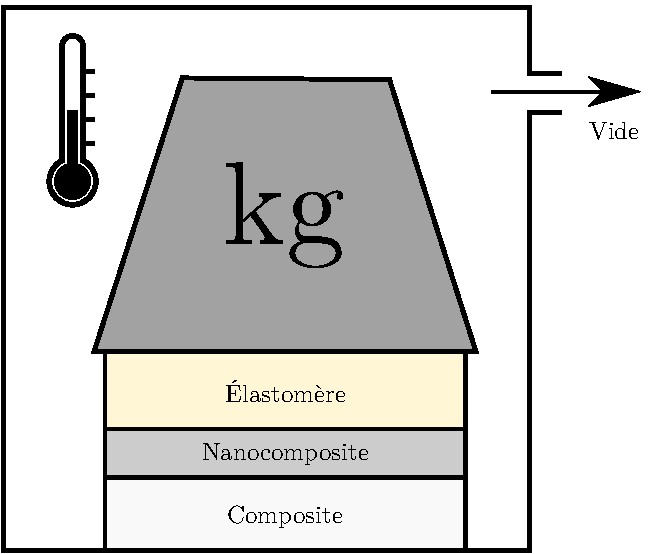
\includegraphics[scale=0.6]{schema_soudure_etuve.pdf}
	\caption{Schéma du procédé de soudage dans une étuve}
	\label{fig:schema_soudure_etuve}
\end{figure}

La seconde méthode utilisée était un soudage dans une presse chauffante manuelle (Fig. \ref{fig:schema_soudure_presse}). 
Durant ce test, un empilement symétrique en sandwich avec deux échantillons de composite et de nanocomposite ainsi qu'un échantillon d'élastomère au centre était positionné entre deux plaques métalliques. 
La presse était préchauffée à la température désirée avant d'insérer l'empilement. 
Lorsque les plateaux de la presse atteignent à la température de consigne, une pression est ensuite appliquée sur l'empilement pour le consolider. 
Après 10 minutes, le chauffage de la presse est arrêté et un ventilateur est utilisé pour accélérer le refroidissement du montage. 
Les échantillons sont retirés de la presse une fois qu'ils sont refroidis. 

\begin{figure}[h]
	\centering
	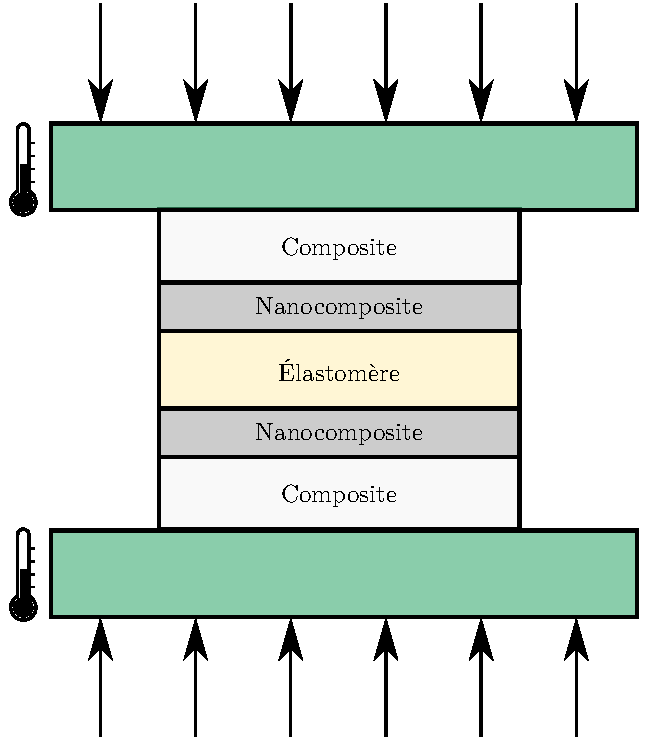
\includegraphics[scale=0.6]{schema_soudure_presse.pdf}
	\caption{Schéma du procédé de soudage à la presse chauffante}
	\label{fig:schema_soudure_presse}
\end{figure}

Suite aux premiers résultats, la possibilité de souder l'élastomère a ensuite été évalué à l'aide du montage de soudage. 
Dans ce dernier, une couche d'élastomère est déposée sur un élément chauffant nanocomposite reposant sur un adhérent de composite. 
L'empilement était déposé sur une céramique isolante avant qu'un autre morceau de céramique ne soit positionné au-dessus de la soudure. 
Les vérins étaient ensuite abaissés pour appliquer une pression sur la zone soudée ainsi que sur les électrodes en contact avec le nanocomposite. 
La quantité de courant et le voltage appliqués durant les essais de soudage ont été contrôlés afin de maintenir une puissance électrique surfacique constante tout au long de chaque test. 

Deux modes de soudures distincts ont été évalués (Fig. \ref{fig:schema_processus_soudure_resistance}). 
\begin{enumerate}
	\item Les soudures des deux côtés de l'élément chauffant nanocomposite, soit la soudure entre le composite et le nanocomposite ainsi que la soudure entre l'élastomère et le nanocomposite ont été réalisés en une seule étape. 
	Ces essais visaient à produire une soudure multimatériaux complète en une seule étape. 
	\item Les soudures ont été réalisées en deux étapes. 
	Une première soudure est réalisée entre le composite et le nanocomposite. 
	Une seconde soudure entre le nanocomposite et l'élastomère est ensuite réalisée en appliquant, de nouveau, un courant électrique dans le nanocomposite déjà soudé au composite. 
	Ce second mode de soudage avait pour but d'employer des conditions d'opération différentes pour chaque combinaison de matériau. 
\end{enumerate}

\begin{figure}[h]
	\centering
	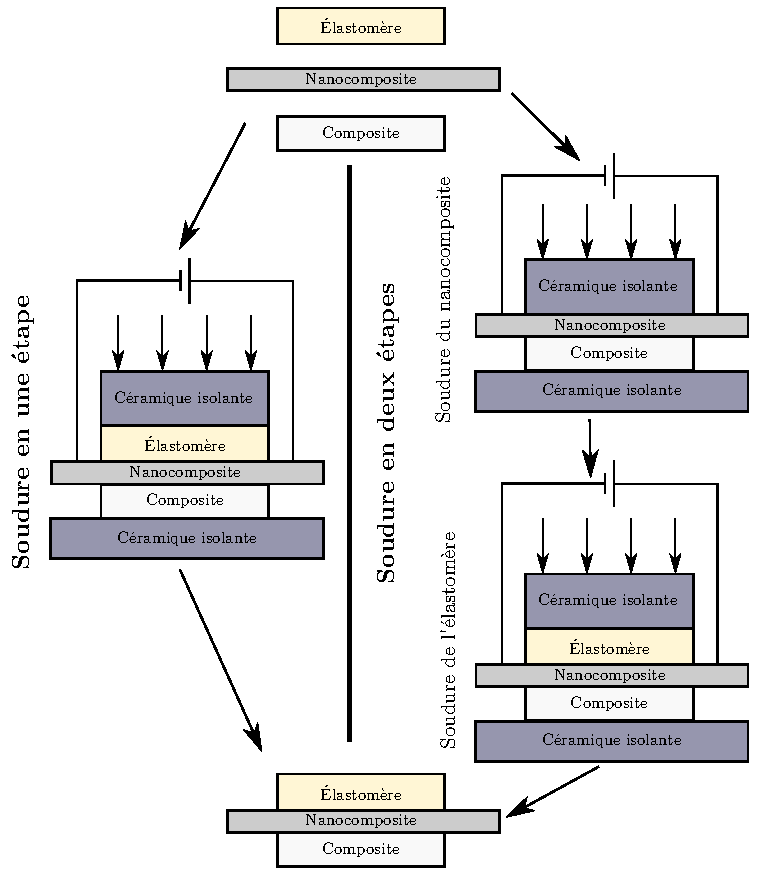
\includegraphics[scale=1]{schema_processus_soudure_resistance.pdf}
	\caption{Schéma du procédé de soudage par résistance montrant les processus en une étape et en deux étapes}
	\label{fig:schema_processus_soudure_resistance}
\end{figure}

Lors du soudage des échantillons pour les essais de caractérisation mécanique, l'élément chauffant nanocomposite est positionné en retrait du bout de l'adhérent d'une distance d'environ 1 à \SI[locale=FR]{2}{\milli\metre}. 
L'élastomère est également positionné de façon à obtenir un retrait de 1 à \SI[locale=FR]{2}{\milli\metre} avec le bout de l'échantillon. 

\subsection{Caractérisation mécanique des joints soudés}

La résistance des soudures a été évaluée selon leur géométrie. 
Les essais dans l'étuve ou sous presse n'avaient pas une géométrie propice à des essais de caractérisation mécanique. 
Dans ces cas particuliers, la soudure était évaluée par pelage manuel du joint. 
Si nécessaire, des outils étaient utilisés pour tenter de décoller les faciès en contact. 
Après la séparation des faciès, une observation visuelle des joints, parfois suivie d'une observation au microscope optique, permet de juger de la qualité du joint. 

\begin{figure}[h]
	\centering
	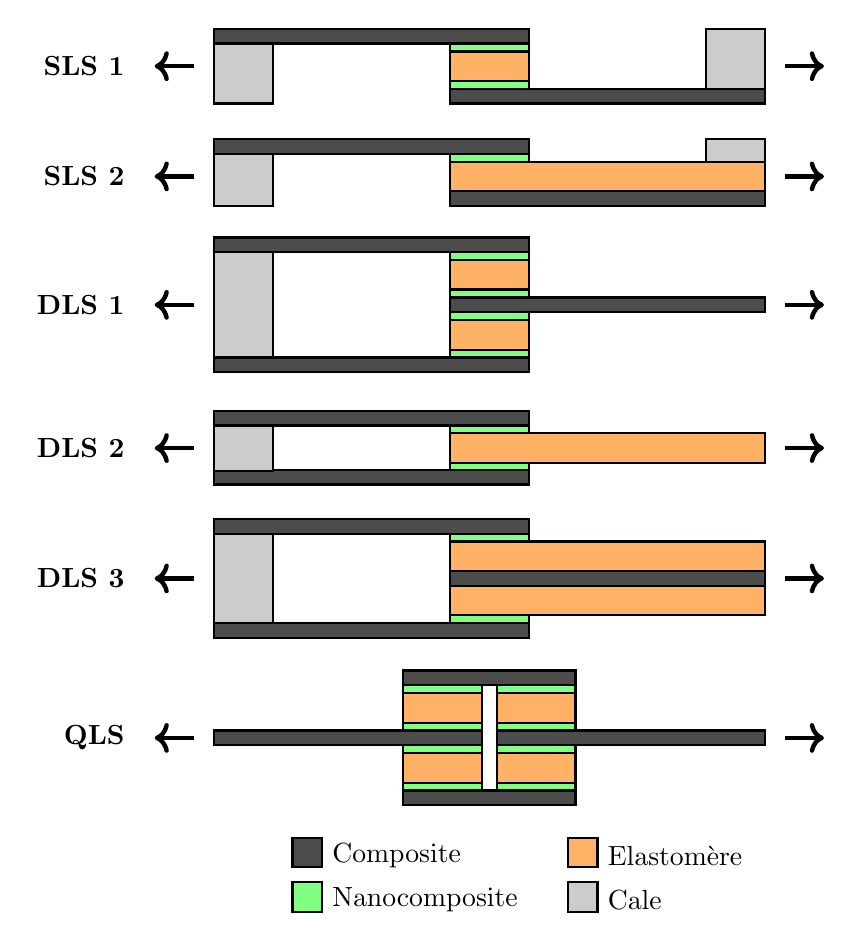
\begin{tikzpicture}[scale=0.5, thick]

%Dimensons générales
\def \overlap{2}
\def \espacevert{1}

%Dimensions composite
\def \lcomp{8}
\def \tcomp{0.375}

%Épaisseur de l'élément résistif
\def \tele{0.2}

%Épaisseur de l'élastomère
\def \tela{0.75}

%Dimensions de la calle
\def \lcalle{1.5}

%Position et taille des annotations
\def \lforce{1}
\def \gapforce{0.5}
\def \gaptexte{0.375}
\def \legende{0.75}
\def \gapscie{0.375}
\def \midgap{0.375}

%Couleurs
\def \colcomp{black!70}
\def \colele{green!50}
\def \colelas{orange!60}
\def \colcalle{black!20}


%\begin{scope}[shift={(0,21)}]
%	%Plaques
%	\draw[black,fill=\colcomp] (0,0) -- ++(0,\tcomp) -- ++(\lcomp,0) -- ++(0,-\tcomp) -- cycle; %Single shear haut
%	\draw[black,fill=\colcomp] (\lcomp-\overlap,-\tele-\tcomp) -- ++(0,\tcomp) -- ++(\lcomp,0) -- ++(0,-\tcomp) -- cycle; %Single shear bas
%	
%	%Éléments chauffants
%	\draw[black,fill=\colele] (\lcomp-\overlap,-\tele) -- ++(0,\tele) -- ++(\overlap,0) -- ++(0,-\tele) -- cycle; %Single shear
%	
%	%Calles
%	\draw[black,fill=\colcalle] (0,0) -- ++(0,-\tele-\tcomp) -- ++(\lcalle,0) -- ++(0,\tele+\tcomp) -- cycle; % calle 1
%	\draw[black,fill=\colcalle] (2*\lcomp-\overlap-\lcalle,\tcomp) -- ++(0,-\tele-\tcomp) -- ++(\lcalle,0) -- ++(0,\tele+\tcomp) -- cycle; % calle 2
%	
%	%Lignes de force
%	\begin{scope}[ultra thick]
%	\draw [->] (-\gapforce,-.5*\tele) -- ++(-\lforce,0);
%	\draw [->] (2*\lcomp-\overlap+\gapforce,-.5*\tele) -- ++(\lforce,0);
%	\end{scope}
%	
%	%Identification de l'éprouvette
%	\draw (-\lforce-2*\gapforce,-.5*\tele) node[left]{\textbf{SLS}};
%\end{scope}

\begin{scope}[shift={(0,18.8)}]
	%Plaques
	\draw[black,fill=\colcomp] (0,0) -- ++(0,\tcomp) -- ++(\lcomp,0) -- ++(0,-\tcomp) -- cycle; %single shear haut 1
	\draw[black,fill=\colcomp] (\lcomp-\overlap,-2*\tele-\tcomp-\tela) -- ++(0,\tcomp) -- ++(\lcomp,0) -- ++(0,-\tcomp) -- cycle; %single shear bas 2
	
	%Éléments chauffants
	\draw[black,fill=\colele] (\lcomp-\overlap,-\tele) -- ++(0,\tele) -- ++(\overlap,0) -- ++(0,-\tele) -- cycle; %single shear haut 2
	\draw[black,fill=\colele] (\lcomp-\overlap,-2*\tele-\tela) -- ++(0,\tele) -- ++(\overlap,0) -- ++(0,-\tele) -- cycle; %single shear bas 2
	
	%Élastomère
	\draw[black,fill=\colelas] (\lcomp-\overlap,-\tela-\tele) -- ++(0,\tela) -- ++(\overlap,0) -- ++(0,-\tela) -- cycle; % elastomère 2

	%Calles
	\draw[black,fill=\colcalle] (0,0) -- ++(0,-2*\tele-\tcomp-\tela) -- ++(\lcalle,0) -- ++(0,2*\tele+\tcomp+\tela) -- cycle; % calle 1
	\draw[black,fill=\colcalle] (2*\lcomp-\overlap-\lcalle,\tcomp) -- ++(0,-2*\tele-\tcomp-\tela) -- ++(\lcalle,0) -- ++(0,2*\tele+\tcomp+\tela) -- cycle; % calle 2
	
	%Lignes de force
	\begin{scope}[ultra thick]
	\draw [->] (-\gapforce,-\tele-0.5*\tela) -- ++(-\lforce,0);
	\draw [->] (2*\lcomp-\overlap+\gapforce,-\tele-0.5*\tela) -- ++(\lforce,0);
	\end{scope}
	
	%Identification de l'éprouvette
	\draw (-\lforce-2*\gapforce,-\tele-0.5*\tela) node[left]{\textbf{SLS 1}};
\end{scope}

\begin{scope}[shift={(0,16)}] 
	%Plaques
	\draw[black,fill=\colcomp] (0,0) -- ++(0,\tcomp) -- ++(\lcomp,0) -- ++(0,-\tcomp) -- cycle; %single shear haut 1
	\draw[black,fill=\colcomp] (\lcomp-\overlap,-\tele-\tcomp-\tela) -- ++(0,\tcomp) -- ++(\lcomp,0) -- ++(0,-\tcomp) -- cycle; %single shear bas 2
	
	%Éléments chauffants
	\draw[black,fill=\colele] (\lcomp-\overlap,-\tele) -- ++(0,\tele) -- ++(\overlap,0) -- ++(0,-\tele) -- cycle; %single shear haut 2

	%Élastomère
	\draw[black,fill=\colelas] (\lcomp-\overlap,-\tela-\tele) -- ++(0,\tela) -- ++(\lcomp,0) -- ++(0,-\tela) -- cycle; % elastomère 2

	%Calles
	\draw[black,fill=\colcalle] (0,0) -- ++(0,-\tele-\tcomp-\tela) -- ++(\lcalle,0) -- ++(0,\tele+\tcomp+\tela) -- cycle; % calle 1
	\draw[black,fill=\colcalle] (2*\lcomp-\overlap-\lcalle,\tcomp) -- ++(0,-\tele-\tcomp) -- ++(\lcalle,0) -- ++(0,\tele+\tcomp) -- cycle; % calle 2
	
	%Lignes de force
	\begin{scope}[ultra thick]
	\draw [->] (-\gapforce,-\tele-0.5*\tela) -- ++(-\lforce,0);
	\draw [->] (2*\lcomp-\overlap+\gapforce,-\tele-0.5*\tela) -- ++(\lforce,0);
	\end{scope}
	
	%Identification de l'éprouvette
	\draw (-\lforce-2*\gapforce,-\tele-0.5*\tela) node[left]{\textbf{SLS 2}};
\end{scope}


\begin{scope}[shift={(0,13.5)}]
	%Plaques
	\draw[black,fill=\colcomp] (0,0) -- ++(0,\tcomp) -- ++(\lcomp,0) -- ++(0,-\tcomp) -- cycle; %dual shear haut
	\draw[black,fill=\colcomp] (\lcomp-\overlap,-2*\tele-\tcomp-\tela) -- ++(0,\tcomp) -- ++(\lcomp,0) -- ++(0,-\tcomp) -- cycle; %dual shear milieu
	\draw[black,fill=\colcomp] (0,-2*\tcomp-4*\tele-2*\tela) -- ++(0,\tcomp) -- ++(\lcomp,0) -- ++(0,-\tcomp) -- cycle; %dual shear bas
	
	%Éléments chauffants
	\draw[black,fill=\colele] (\lcomp-\overlap,-\tele) -- ++(0,\tele) -- ++(\overlap,0) -- ++(0,-\tele) -- cycle; %dual shear haut 1
	\draw[black,fill=\colele] (\lcomp-\overlap,-2*\tele-\tela) -- ++(0,\tele) -- ++(\overlap,0) -- ++(0,-\tele) -- cycle; %dual shear haut 2
	\draw[black,fill=\colele] (\lcomp-\overlap,-3*\tele-\tela-\tcomp) -- ++(0,\tele) -- ++(\overlap,0) -- ++(0,-\tele) -- cycle; %dual shear bas 1
	\draw[black,fill=\colele] (\lcomp-\overlap,-4*\tele-2*\tela-\tcomp) -- ++(0,\tele) -- ++(\overlap,0) -- ++(0,-\tele) -- cycle; %dual shear bas 2
	
	%Élastomère
	\draw[black,fill=\colelas] (\lcomp-\overlap,-\tela-\tele) -- ++(0,\tela) -- ++(\overlap,0) -- ++(0,-\tela) -- cycle; % elastomère haut
	\draw[black,fill=\colelas] (\lcomp-\overlap,-2*\tela-3*\tele-\tcomp) -- ++(0,\tela) -- ++(\overlap,0) -- ++(0,-\tela) -- cycle; % elastomère bas
	
	%Calle
	\draw[black,fill=\colcalle] (0,0) -- ++(0,-4*\tele-2*\tela-\tcomp) -- ++(\lcalle,0) -- ++(0,4*\tele+2*\tela+\tcomp) -- cycle; % calle
	
	%Lignes de force
	\begin{scope}[ultra thick]
	\draw [->] (-\gapforce,-2*\tele-\tela-0.5*\tcomp) -- ++(-\lforce,0);
	\draw [->] (2*\lcomp-\overlap+\gapforce,-2*\tele-\tela-0.5*\tcomp) -- ++(\lforce,0);
	\end{scope}
	
	%Identification de l'éprouvette
	\draw (-\lforce-2*\gapforce,-2*\tele-\tela-0.5*\tcomp) node[left]{\textbf{DLS 1}};
\end{scope}


\begin{scope}[shift={(0,9.1)}] 
	%Plaques
	\draw[black,fill=\colcomp] (0,0) -- ++(0,\tcomp) -- ++(\lcomp,0) -- ++(0,-\tcomp) -- cycle; %dual shear haut
	\draw[black,fill=\colcomp] (0,-2*\tcomp-\tela) -- ++(0,\tcomp) -- ++(\lcomp,0) -- ++(0,-\tcomp) -- cycle; %dual shear bas
	
	%Éléments chauffants
	\draw[black,fill=\colele] (\lcomp-\overlap,-\tele) -- ++(0,\tele) -- ++(\overlap,0) -- ++(0,-\tele) -- cycle; %dual shear haut 1
	\draw[black,fill=\colele] (\lcomp-\overlap,-\tela-\tcomp) -- ++(0,\tele) -- ++(\overlap,0) -- ++(0,-\tele) -- cycle; %dual shear bas 2
	
	%Élastomère
	\draw[black,fill=\colelas] (\lcomp-\overlap,-\tela-\tele) -- ++(0,\tela) -- ++(\lcomp,0) -- ++(0,-\tela) -- cycle; % elastomère haut
	
	%Calle
	\draw[black,fill=\colcalle] (0,0) -- ++(0,-2*\tele-\tela) -- ++(\lcalle,0) -- ++(0,2*\tele+\tela) -- cycle; % calle
	
	%Lignes de force
	\begin{scope}[ultra thick]
	\draw [->] (-\gapforce,-\tele-0.5*\tela) -- ++(-\lforce,0);
	\draw [->] (2*\lcomp-\overlap+\gapforce,-\tele-0.5*\tela) -- ++(\lforce,0);
	\end{scope}
	
	%Identification de l'éprouvette
	\draw (-\lforce-2*\gapforce,-\tele-0.5*\tela) node[left]{\textbf{DLS 2}};
\end{scope}


\begin{scope}[shift={(0,6.35)}] 
	%Plaques
	\draw[black,fill=\colcomp] (0,0) -- ++(0,\tcomp) -- ++(\lcomp,0) -- ++(0,-\tcomp) -- cycle; %dual shear haut
	\draw[black,fill=\colcomp] (\lcomp-\overlap,-\tele-\tcomp-\tela) -- ++(0,\tcomp) -- ++(\lcomp,0) -- ++(0,-\tcomp) -- cycle; %dual shear milieu
	\draw[black,fill=\colcomp] (0,-2*\tcomp-2*\tele-2*\tela) -- ++(0,\tcomp) -- ++(\lcomp,0) -- ++(0,-\tcomp) -- cycle; %dual shear bas
	
	%Éléments chauffants
	\draw[black,fill=\colele] (\lcomp-\overlap,-\tele) -- ++(0,\tele) -- ++(\overlap,0) -- ++(0,-\tele) -- cycle; %dual shear haut 1
	\draw[black,fill=\colele] (\lcomp-\overlap,-2*\tele-2*\tela-\tcomp) -- ++(0,\tele) -- ++(\overlap,0) -- ++(0,-\tele) -- cycle; %dual shear bas 2
	
	%Élastomère
	\draw[black,fill=\colelas] (\lcomp-\overlap,-\tela-\tele) -- ++(0,\tela) -- ++(\lcomp,0) -- ++(0,-\tela) -- cycle; % elastomère haut
	\draw[black,fill=\colelas] (\lcomp-\overlap,-2*\tela-1*\tele-\tcomp) -- ++(0,\tela) -- ++(\lcomp,0) -- ++(0,-\tela) -- cycle; % elastomère bas
	
	%Calle
	\draw[black,fill=\colcalle] (0,0) -- ++(0,-2*\tele-2*\tela-\tcomp) -- ++(\lcalle,0) -- ++(0,2*\tele+2*\tela+\tcomp) -- cycle; % calle
	
	%Lignes de force
	\begin{scope}[ultra thick]
	\draw [->] (-\gapforce,-\tele-\tela-0.5*\tcomp) -- ++(-\lforce,0);
	\draw [->] (2*\lcomp-\overlap+\gapforce,-\tele-\tela-0.5*\tcomp) -- ++(\lforce,0);
	\end{scope}
	
	%Identification de l'éprouvette
	\draw (-\lforce-2*\gapforce,-\tele-\tela-0.5*\tcomp) node[left]{\textbf{DLS 3}};
\end{scope}


\begin{scope}[shift={(0,2.5)}]
	%Plaques
	\draw[black,fill=\colcomp] (\lcomp-1.5*\overlap-0.5*\midgap,0) -- ++(0,\tcomp) -- ++(2*\overlap+\midgap,0) -- ++(0,-\tcomp) -- cycle; %quad shear haut
	\draw[black,fill=\colcomp] (0,-2*\tele-\tcomp-\tela) -- ++(0,\tcomp) -- ++(\lcomp-0.5*\overlap-0.5*\midgap,0) -- ++(0,-\tcomp) -- cycle; %quad shear milieu 1
	\draw[black,fill=\colcomp] (\lcomp-0.5*\overlap+0.5*\midgap,-2*\tele-\tcomp-\tela) -- ++(0,\tcomp) -- ++(\lcomp-0.5*\overlap-0.5*\midgap,0) -- ++(0,-\tcomp) -- cycle; %quad shear milieu 2
	\draw[black,fill=\colcomp] (\lcomp-1.5*\overlap-0.5*\midgap,-2*\tcomp-4*\tele-2*\tela) -- ++(0,\tcomp) -- ++(2*\overlap+\midgap,0) -- ++(0,-\tcomp) -- cycle; %quad shear bas
	
	%Éléments chauffants 
	
	%gauche
	\draw[black,fill=\colele] (\lcomp-1.5*\overlap-0.5*\midgap,-\tele) -- ++(0,\tele) -- ++(\overlap,0) -- ++(0,-\tele) -- cycle; %quad shear haut 1
	\draw[black,fill=\colele] (\lcomp-1.5*\overlap-0.5*\midgap,-2*\tele-\tela) -- ++(0,\tele) -- ++(\overlap,0) -- ++(0,-\tele) -- cycle; %quad shear haut 2
	\draw[black,fill=\colele] (\lcomp-1.5*\overlap-0.5*\midgap,-3*\tele-\tela-\tcomp) -- ++(0,\tele) -- ++(\overlap,0) -- ++(0,-\tele) -- cycle; %quad shear bas 1
	\draw[black,fill=\colele] (\lcomp-1.5*\overlap-0.5*\midgap,-4*\tele-2*\tela-\tcomp) -- ++(0,\tele) -- ++(\overlap,0) -- ++(0,-\tele) -- cycle; %quad shear bas 2
	
	%droite
	\draw[black,fill=\colele] (\lcomp-0.5*\overlap+0.5*\midgap,-\tele) -- ++(0,\tele) -- ++(\overlap,0) -- ++(0,-\tele) -- cycle; %quad shear haut 1
	\draw[black,fill=\colele] (\lcomp-0.5*\overlap+0.5*\midgap,-2*\tele-\tela) -- ++(0,\tele) -- ++(\overlap,0) -- ++(0,-\tele) -- cycle; %quad shear haut 2
	\draw[black,fill=\colele] (\lcomp-0.5*\overlap+0.5*\midgap,-3*\tele-\tela-\tcomp) -- ++(0,\tele) -- ++(\overlap,0) -- ++(0,-\tele) -- cycle; %quad shear bas 1
	\draw[black,fill=\colele] (\lcomp-0.5*\overlap+0.5*\midgap,-4*\tele-2*\tela-\tcomp) -- ++(0,\tele) -- ++(\overlap,0) -- ++(0,-\tele) -- cycle; %quad shear bas 2
	
	%Élastomère
	
	%gauche
	\draw[black,fill=\colelas] (\lcomp-1.5*\overlap-0.5*\midgap,-\tela-\tele) -- ++(0,\tela) -- ++(\overlap,0) -- ++(0,-\tela) -- cycle; % elastomère haut 1
	\draw[black,fill=\colelas] (\lcomp-1.5*\overlap-0.5*\midgap,-2*\tela-3*\tele-\tcomp) -- ++(0,\tela) -- ++(\overlap,0) -- ++(0,-\tela) -- cycle; % elastomère bas 1
	
	%droite
	\draw[black,fill=\colelas] (\lcomp-0.5*\overlap+0.5*\midgap,-\tela-\tele) -- ++(0,\tela) -- ++(\overlap,0) -- ++(0,-\tela) -- cycle; % elastomère haut 1
	\draw[black,fill=\colelas] (\lcomp-0.5*\overlap+0.5*\midgap,-2*\tela-3*\tele-\tcomp) -- ++(0,\tela) -- ++(\overlap,0) -- ++(0,-\tela) -- cycle; % elastomère bas 1
	
	%Lignes de force
	\begin{scope}[ultra thick]
	\draw [->] (-\gapforce,-2*\tele-\tela-0.5*\tcomp) -- ++(-\lforce,0);
	\draw [->] (2*\lcomp-\overlap+\gapforce,-2*\tele-\tela-0.5*\tcomp) -- ++(\lforce,0);
	\end{scope}
	
	%Identification de l'éprouvette
	\draw (-\lforce-2*\gapforce,-2*\tele-\tela-0.5*\tcomp) node[left]{\textbf{QLS}};
\end{scope}

\begin{scope}[shift={(2,0)}]
	%Legende
	\draw [black, fill=\colcomp] (0,-\espacevert-1.5*\legende) rectangle ++(\legende,\legende);
	\draw (\legende,-\espacevert-\legende-.075) node[right]{Composite};

	\draw [black, fill=\colele] (0,-\espacevert-3*\legende) rectangle ++(\legende,\legende);
	\draw (\legende,-\espacevert-2.5*\legende-.075) node[right]{Nanocomposite};

	\draw [black, fill=\colelas] (7,-\espacevert-1.5*\legende) rectangle ++(\legende,\legende);
	\draw (7+\legende,-\espacevert-\legende-.075) node[right]{Elastomère};

	\draw [black, fill=\colcalle] (7,-\espacevert-3*\legende) rectangle ++(\legende,\legende);
	\draw (7+\legende,-\espacevert-2.5*\legende-.075) node[right]{Cale};

\end{scope}

\end{tikzpicture}

	\caption{Géométries en simple cisaillement (SLS), en double cisaillement (DLS) et en quadruple cisaillement (QLS) évaluées pour les essais de caractérisation mécaniques de la jonction flexible}
	\label{fig:geometrie_echantillons}
\end{figure}

Pour de déterminer la géométrie optimale des échantillons afin d'évaluer la résistance des joints soudés avec le montage de soudage par résistance, des modèles par éléments finis ont été développés. 
Plusieurs géométries d'échantillons comprenant des joints en simple cisaillement (SLS), des joints en double cisaillement (DLS) et des joints en quadruple cisaillement (QLS) ont été évaluées (Fig. \ref{fig:geometrie_echantillons}). 
Avant de procéder à la modélisation, une analyse des capacités de production a déterminé que les joints évalués devraient autant que possible n'avoir qu'une seule soudure. 
Également, la solution retenu devait limiter la déformation en rotation du joint causée par l'épaisseur de l'élastomère. 

Il a été jugé que les géométries DSL 1 et QLS n'étaient pas des solutions désirables en raison du nombre de soudures à réaliser. 
De plus, la solution SLS 1, nécessitant 2 soudures et causant une déformation en rotation du joint, ne présentait aucun avantage par rapport à la solution SLS 2 qui ne nécessite qu'une seule soudure. 

Des modèles par éléments finis ont été établis pour les solutions SLS 2, DLS 2 et DLS 3 dans le logiciel COMSOL Mul\-ti\-phy\-sics\-\textregistered . 
Dans ces modèles, basés sur les propriétés des matériaux, une force était appliquée de façon à simuler un essai mécanique en simple ou en double cisaillement avec des échantillons fixés dans les mors d'une machine de traction. 
L'extrémité d'un des adhérents était fixée et l'extrémité de l'autre était soumise à un chargement dans l'axe de l'échantillon sans possibilité de se déplacer ou de se déformer dans une autre direction. 

L'analyse des résultats pour la solution DSL 2, avec une couche d'élastomère servant d'adhérent, a démontré que la fabrication de cet échantillon nécessiterait un adhérent élastomère avec une épaisseur d'au moins \SI[locale=FR]{15}{\milli\metre} afin d'obtenir une rupture dans le joint plutôt qu'une rupture en tension de l'adhérent. 
Cette analyse ne prend pas en compte l'effet local des mâchoires. 
Une rupture pourrait se produire dans cette zone. 
Le tout est sans compter la difficulté de produire un échantillon sans défauts de \SI[locale=FR]{15}{\milli\metre} d'épaisseur. 
Basé sur ces résultats, la géométrie d'échantillon DSL 2 a été mise de côté.

\begin{figure}[h]
	\centering
	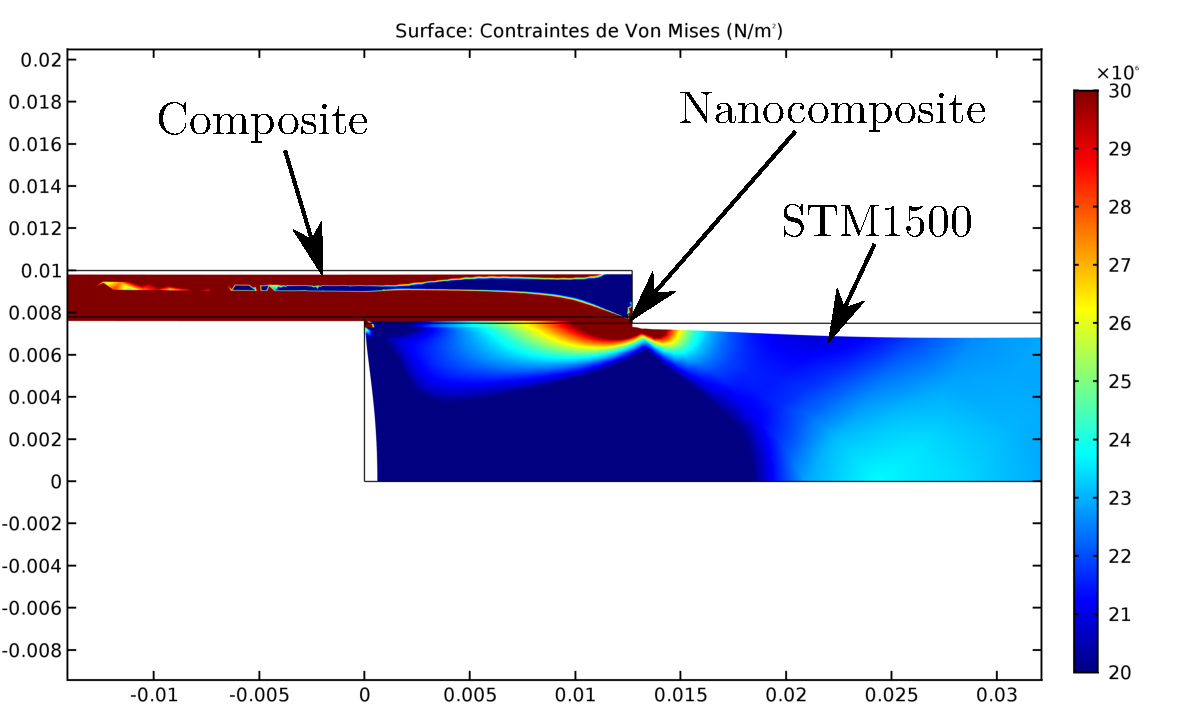
\includegraphics[width=0.6\textwidth]{DLS_Comp-TPE.pdf}
	\caption{Déformations et champ de contrainte pour un échantillon DLS 2 avec une couche d'élastomère de \SI[locale=FR]{15}{\milli\metre} d'épaisseur, un plan de symétrie au milieu de l'élastomère est employé pour simplifier le modèle}
	\label{fig:DLS_comp_TPE}
\end{figure}

\begin{figure}[h!]
	\centering
	\subfigure[]
	{\label{fig:DLS_metal_1mm} 								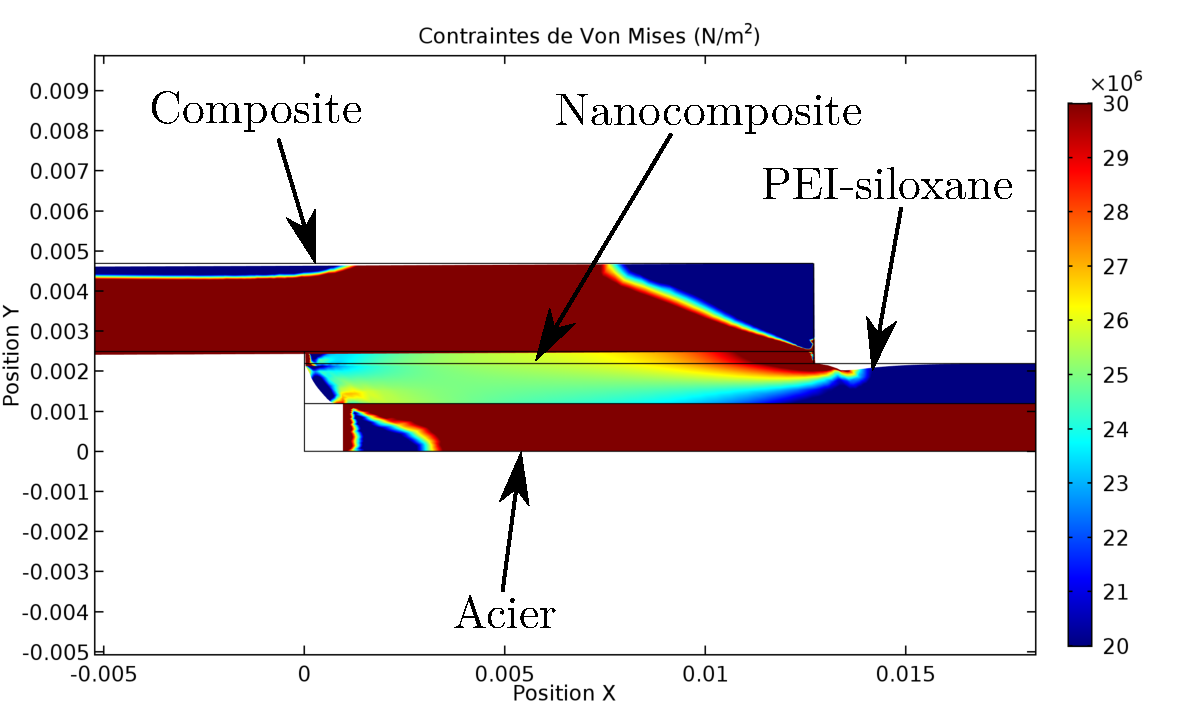
\includegraphics[width=0.6\textwidth]{DLS_Comp-TPE(metal)_1mm.pdf}
	} \\
	\subfigure[]
	{\label{fig:DLS_metal_2mm}
		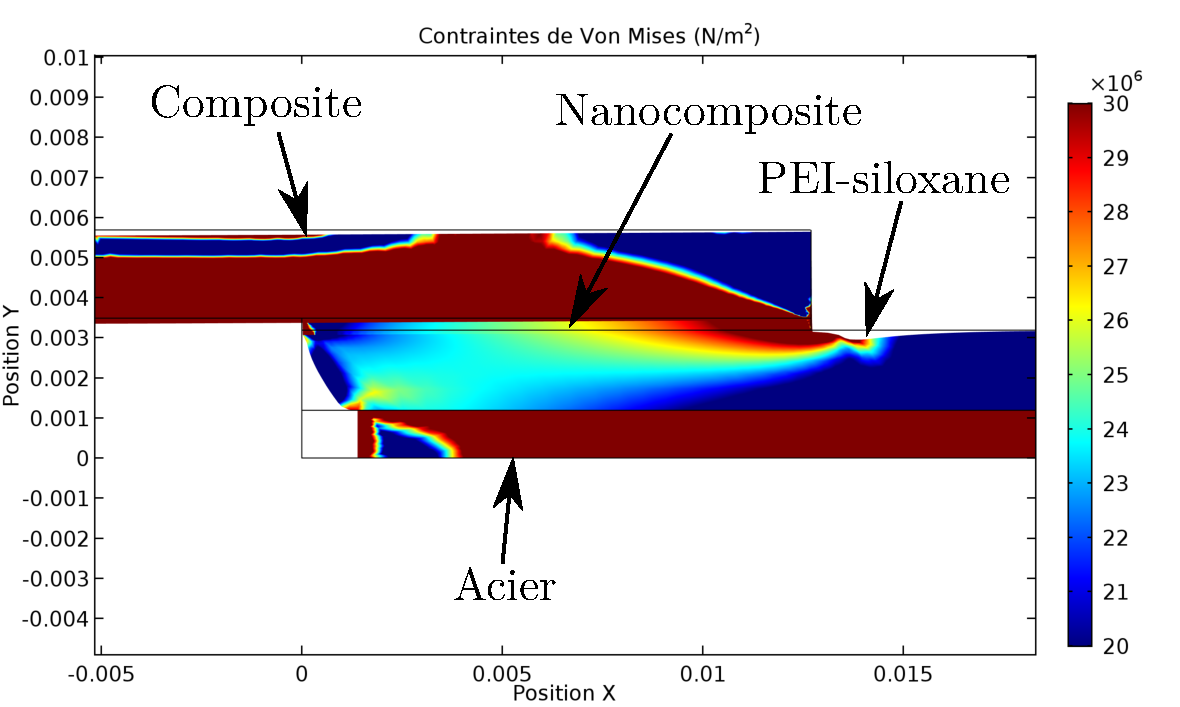
\includegraphics[width=0.6\textwidth]{DLS_Comp-TPE(metal)_2mm.pdf}
	} \\
	\subfigure[]
	{\label{fig:DLS_metal_5mm}
		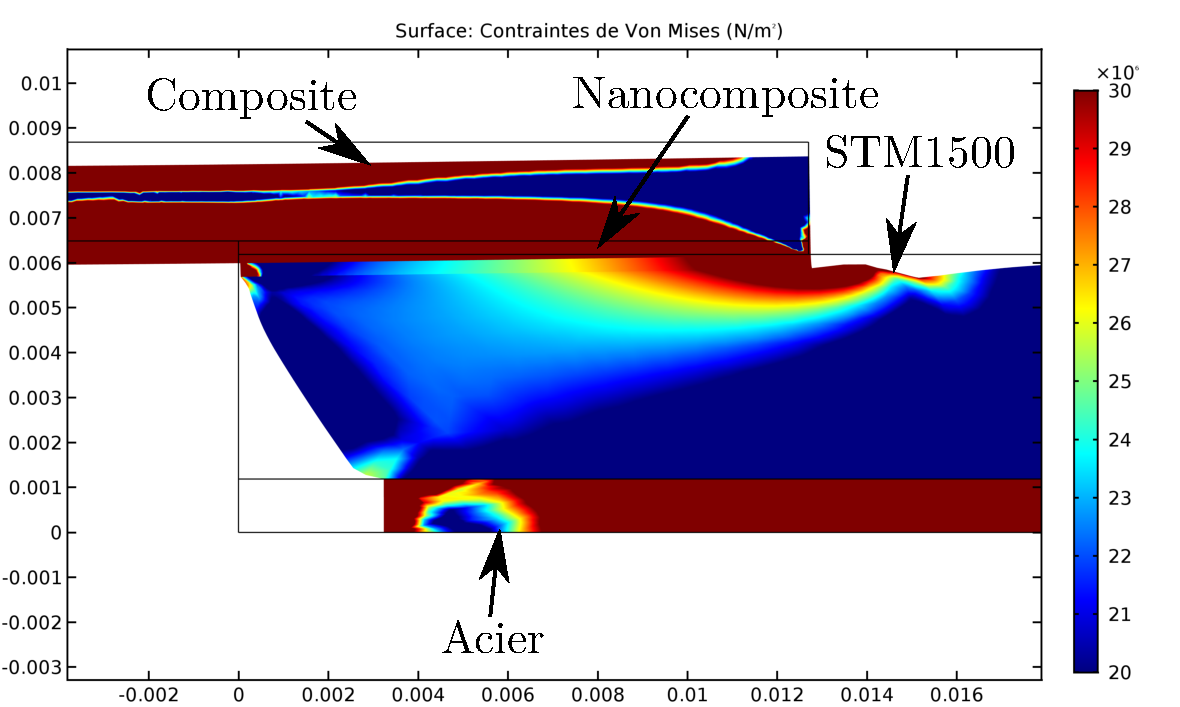
\includegraphics[width=0.6\textwidth]{DLS_Comp-TPE(metal)_5mm.pdf}
	}
	\caption{Analyse de l'effet de l'épaisseur de l'élastomère sur le champ de contrainte dans les échantillons DLS 3, avec un substrat en acier, un plan de symétrie au milieu du substrat en acier est employé pour simplifier le modèle. Champs de contrainte pour des épaisseurs d'élastomère de a) \SI{1}{\milli\metre}, b) \SI{2}{\milli\metre} et c) \SI{5}{\milli\metre}}
	\label{fig:DLS_metal}
\end{figure}

Les prochains modèles ont étudiés la géométrie DSL 3 où des couches d'élastomère sont collées sur un substrat en composite ou en acier (Fig. \ref{fig:DLS_metal}). 
Cette géométrie avait pour but de limiter le transfert de charge au travers de l'élastomère. 
Le principal élément évalué avec ces simulations est l'effet de l'épaisseur de l'élastomère sur le champ de contrainte. 
Il est important d'éviter les effets de bord causés par le substrat rigide lorsqu'une couche d'élastomère trop mince est utilisée. 
On peut voir qu'une épaisseur d'élastomère de \SI[locale=FR]{1}{\milli\metre} (Fig. \ref{fig:DLS_metal_1mm}) produit un champ de contrainte qui est fortement affecté par la présence d'un substrat en acier. 
Lorsque l'épaisseur de l'élastomère est augmenté à 2 et \SI[locale=FR]{5}{\milli\metre} (Fig. \ref{fig:DLS_metal_2mm} et \ref{fig:DLS_metal_5mm}), le champ de contrainte est de moins en moins affecté par l'influence du substrat. 
Une épaisseur supérieure à \SI[locale=FR]{2}{\milli\metre} sera suffisante pour minimiser l'effet du substrat en acier sur la jonction soudée. 

\begin{figure}[h]
	\centering
	\subfigure[]
	{\label{fig:SLS_metal_1mm} 								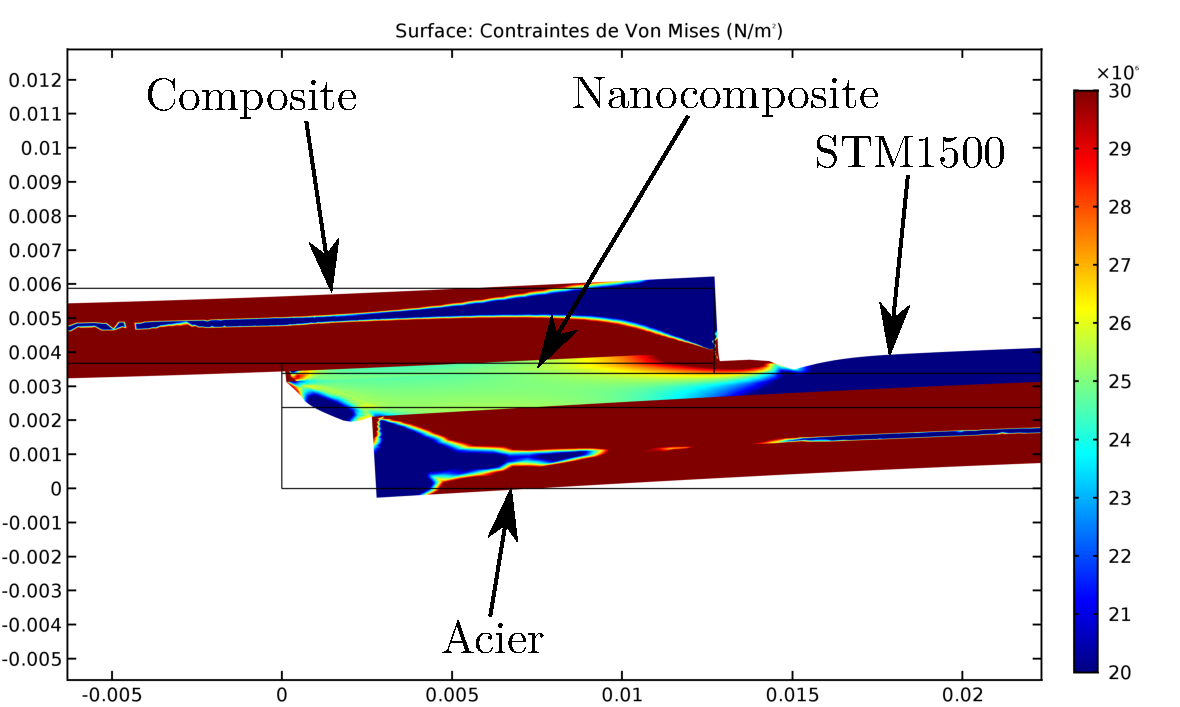
\includegraphics[width=0.6\textwidth]{SLS_Comp-TPE(metal)_1mm.pdf}
	}\qquad
	\subfigure[]
	{\label{fig:SLS_metal_2mm}
		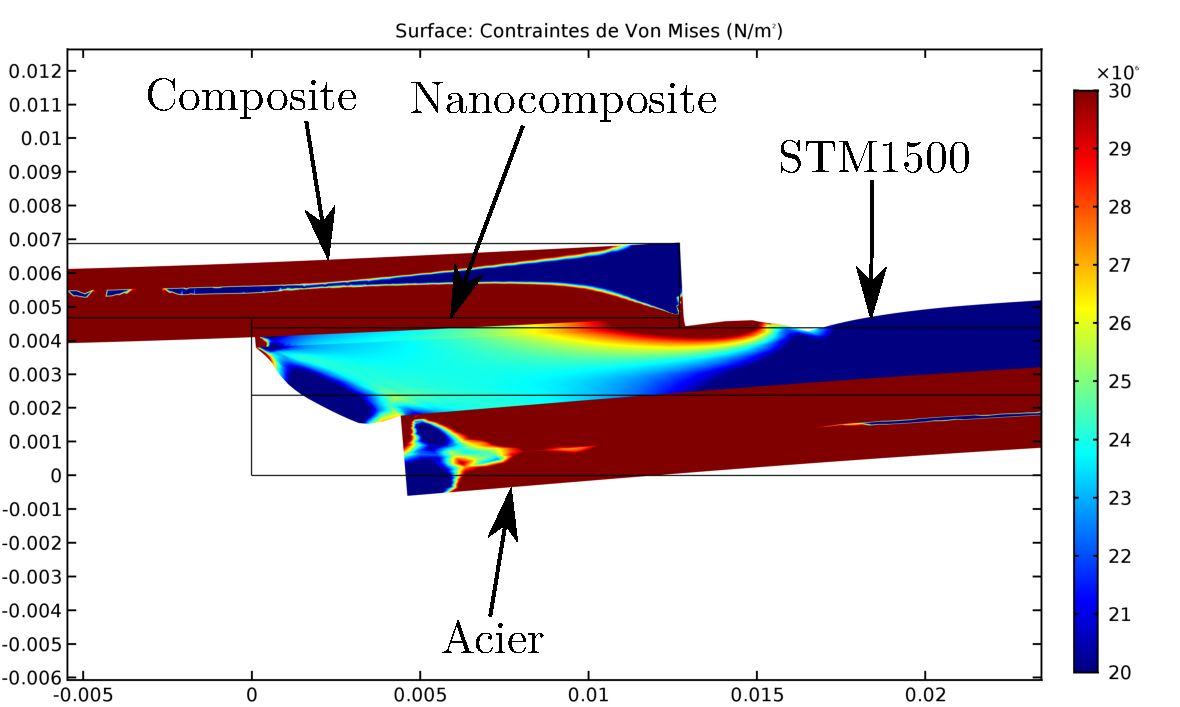
\includegraphics[width=0.6\textwidth]{SLS_Comp-TPE(metal)_2mm.pdf}
	} 
	\subfigure[]
	{\label{fig:SLS_metal_5mm}
		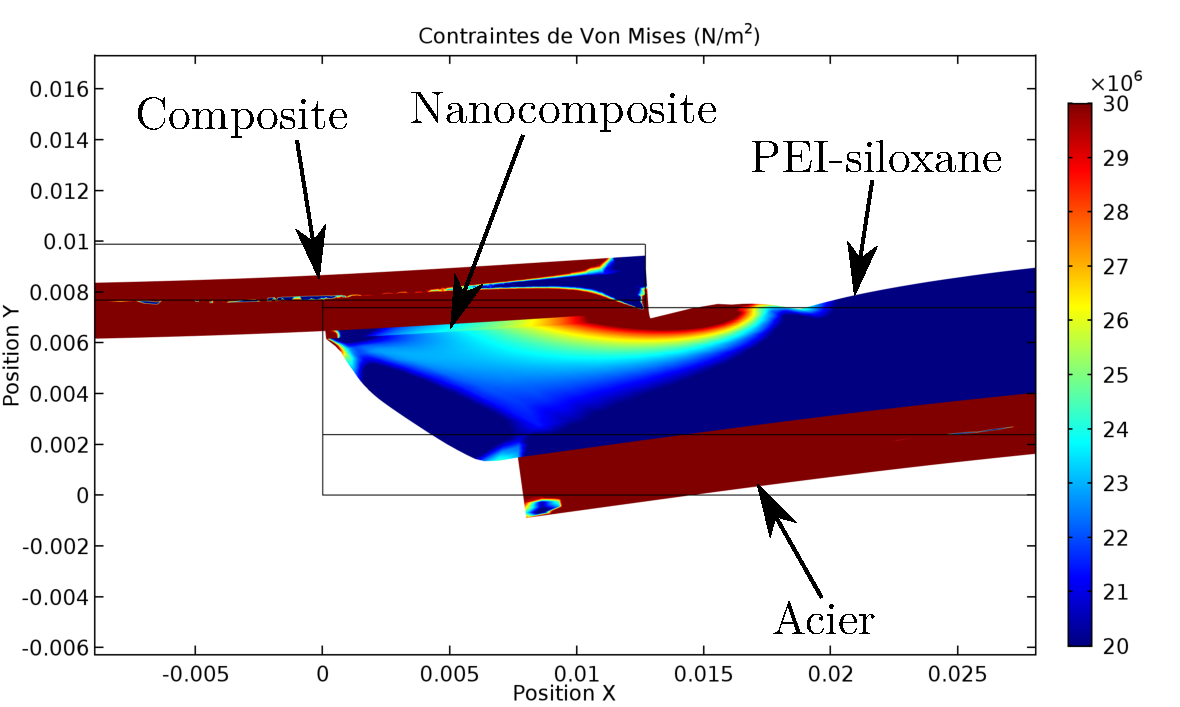
\includegraphics[width=0.6\textwidth]{SLS_Comp-TPE(metal)_5mm.pdf}
	} 
	\caption{Analyse de la rotation et du champ de contrainte dans les échantillons SLS 2, avec un substrat en acier. Champs de contrainte pour des épaisseurs d'élastomère de a) \SI{1}{\milli\metre}, b) \SI{2}{\milli\metre} et c) \SI{5}{\milli\metre}}
	\label{fig:SLS_metal}
\end{figure}

Afin d'évaluer la possibilité d'utiliser une géométrie plus simple à produire pour les échantillons, des modèles par éléments finis ont été développés pour analyser la rotation du joint et le champ de contrainte dans l'élastomère pour la géométrie SLS 2 (Fig. \ref{fig:SLS_metal}). 
Un autre but de ce modèle était de déterminer l'épaisseur requise pour le substrat en acier afin de minimiser les déformations hors du plan.  
Le premier constat lors de l'analyse des résultats est que l'épaisseur de l'élastomère a le même impact sur le champ de contrainte. 
L'évaluation de l'épaisseur nécessaire pour obtenir un champ de contrainte non affecté par le substrat en acier précédemment effectuée pour la géométrie DLS 3 reste donc valide pour cette géométrie, lorsque le substrat en acier possède une rigidité suffisante pour minimiser la rotation du joint. 
Un deuxième constat est qu'une plaque d'acier de \SI[locale=FR]{2.4}{\milli\metre} d'épaisseur permet de minimiser la rotation du joint. 

Au vues de ces analyses, il a été décidé que la performance des joints produits avec le montage de soudage par résistance serait évaluée à l'aide d'un chargement en simple cisaillement entre deux adhérents selon la géométrie SLS 2. 
En raison des moules disponibles, une couche d'élastomère de \SI[locale=FR]{3.18}{\milli\metre} sera utilisée avec un substrat en acier de \SI[locale=FR]{2.4}{\milli\metre}. 
Les adhérents d'élastomère a été collé aux substrats d'acier à l'aide d'une colle époxyde structurelle. 
Des talons ont été installés aux deux extrémités pour faciliter le montage de l'échantillon dans la machine de traction. 
Les essais de caractérisation mécanique ont été réalisés avec une machine Landmark de MTS qui possède une cellule de charge de \SI[locale=FR]{100}{\kilo\newton}. 

\FloatBarrier
\section{Résultats et analyse}

\subsection{Stabilité thermique du nanocomposite}

En parallèle des essais de caractérisation thermique de l'élastomère, la stabilité thermique du nanocomposite a été validée. 
Cette dernière étant en quelque sorte la limite opérationnelle du procédé de soudage, les élastomères ne devraient jamais être exposés à des températures aussi élevées. 
Comme prévu, le PEI du nanocomposite a démontré des signes de dégradation lorsque la température a dépassé \SI[locale=FR]{450}{\celsius} (Fig. \ref{fig:TGA_nanocomposite}). 

\begin{figure}[htb]
	\centering
	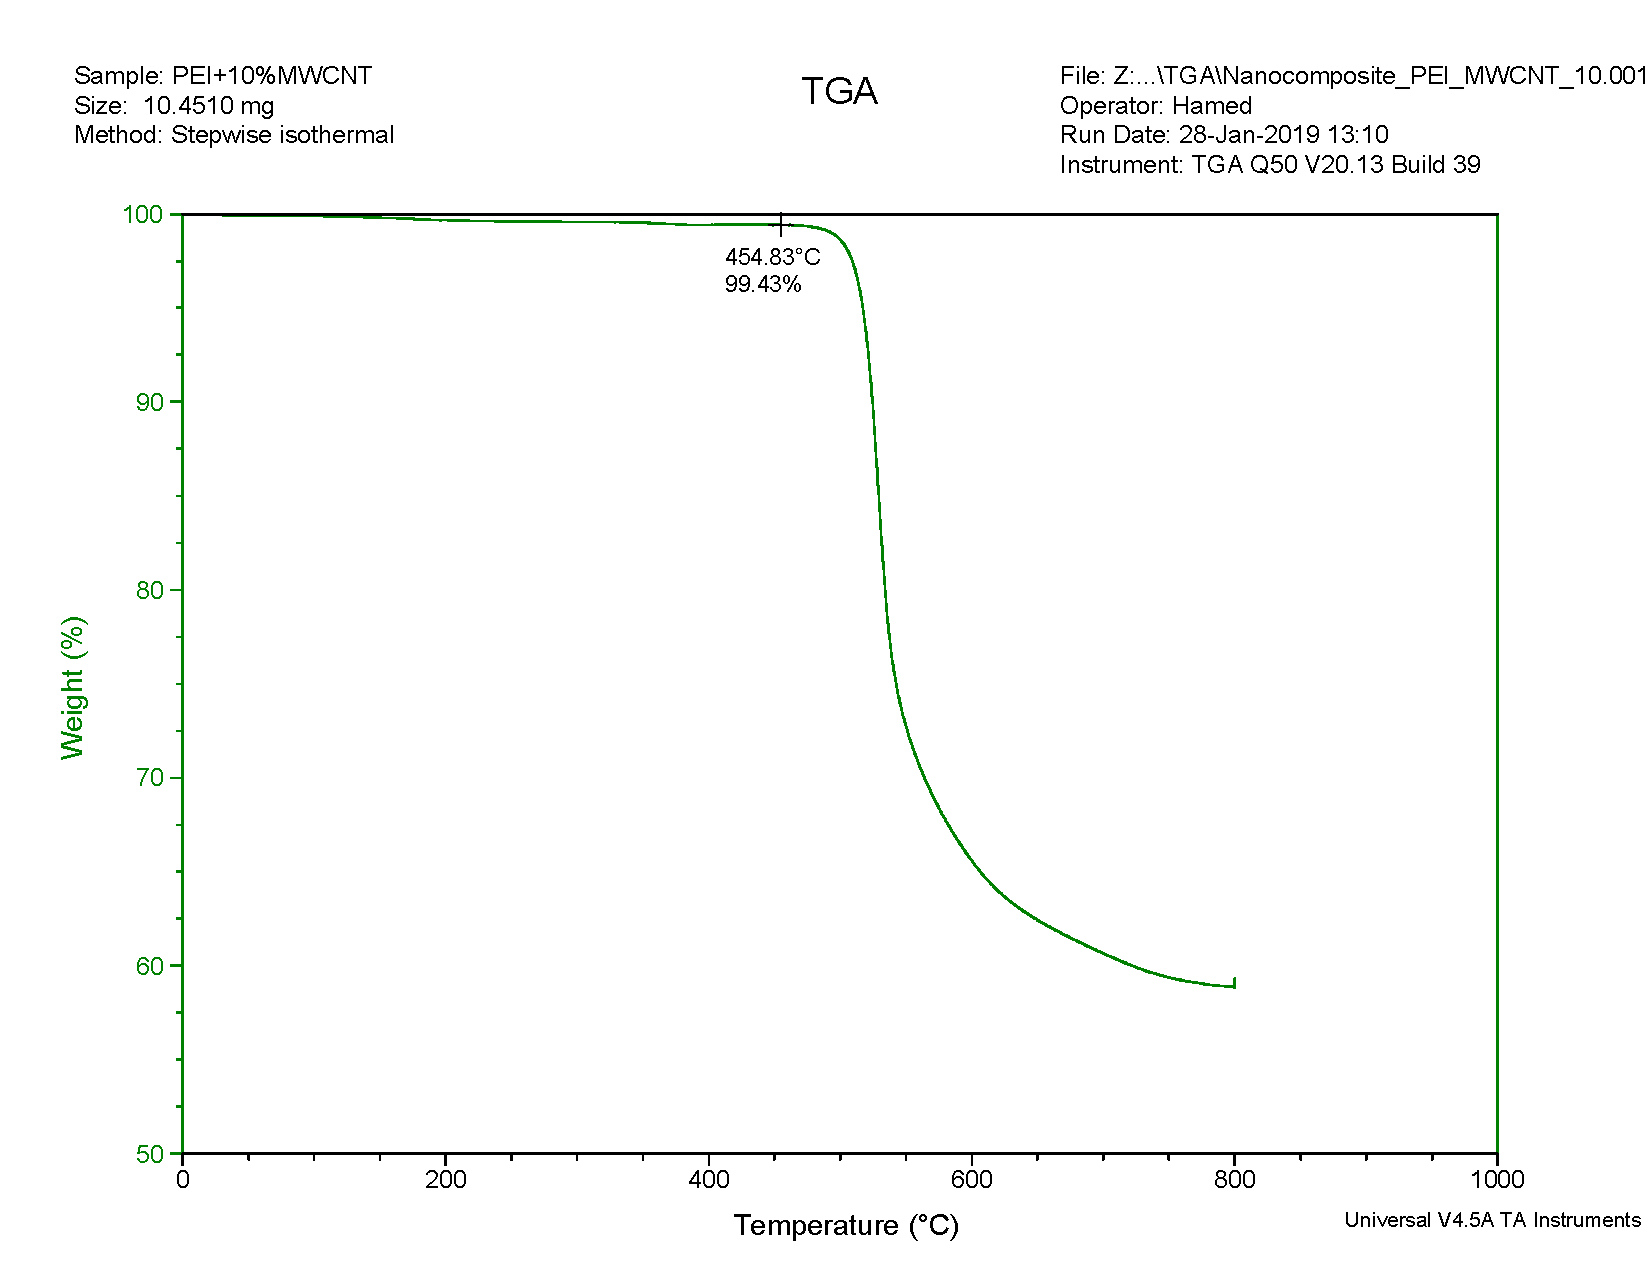
\includegraphics[width=0.95\textwidth]{TGA_nanocomposite.pdf}
	\caption{Résultats en TGA dans l'air pour le nanocomposite}
	\label{fig:TGA_nanocomposite}
\end{figure}

\FloatBarrier
\subsection{Stabilité thermique de l'élastomère}

La stabilité thermique du PEI-siloxane a été évaluée. 
L'élastomère a conservé au moins 99,5\% de sa masse jusqu'à la température de \SI[locale=FR]{360}{\celsius} sous une atmosphère standard (Fig. \ref{fig:TGA_STM1500}). 
La stabilité thermique de cet élastomère est supérieure aux deux autres élastomères étudiés et est suffisamment élevée pour la réalisation d'essais de soudage. 

\begin{figure}[h]
	\centering
	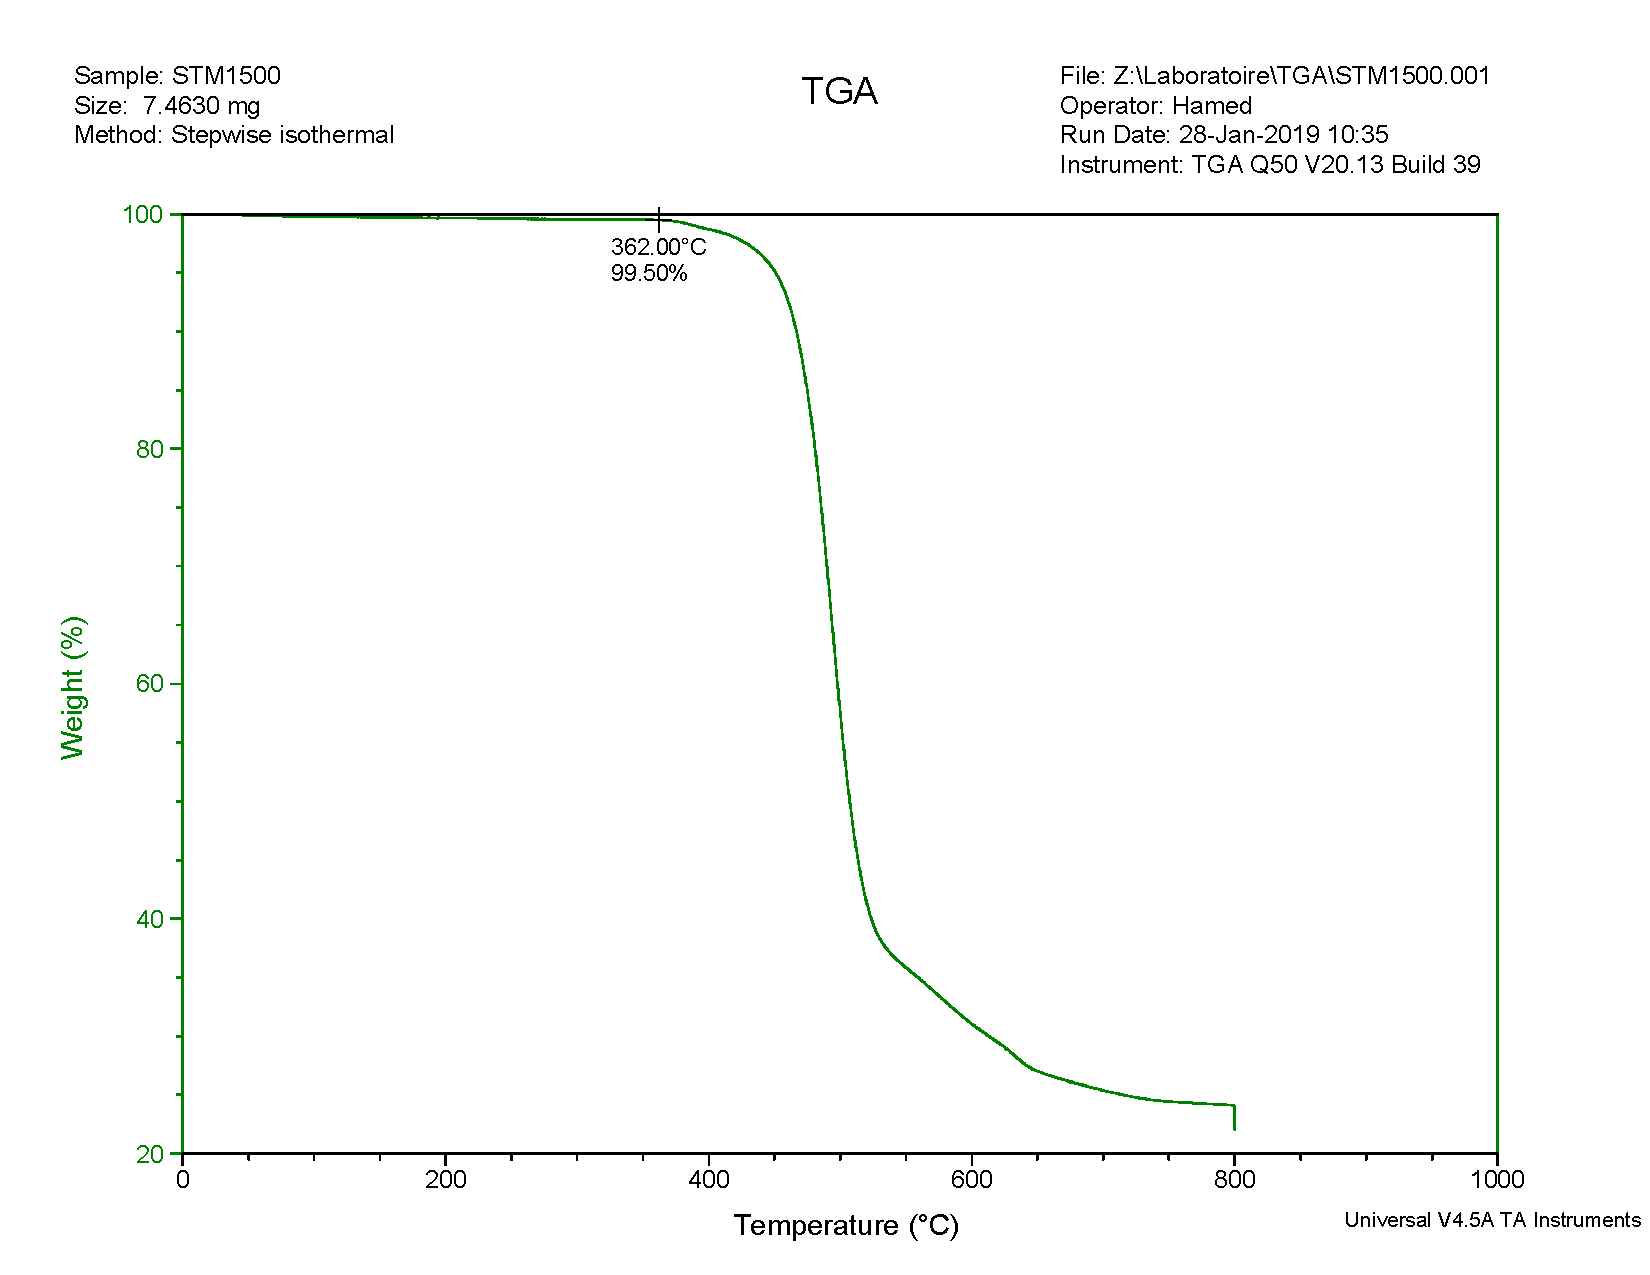
\includegraphics[width=0.95\textwidth]{TGA_STM1500.pdf}
	\caption{Résultats en TGA dans l'air pour le PEI-siloxane}
	\label{fig:TGA_STM1500}
\end{figure}

\FloatBarrier
\subsection{Caractérisation mécanique de l'élastomère}

Les échantillons de PEI-siloxane ont atteint une contrainte à la rupture de \SI[locale=FR]{29}{\mega\pascal} avec une déformation de 250\% (Fig. \ref{fig:STM1500_tension}). 

\begin{figure}[h]
	\centering
	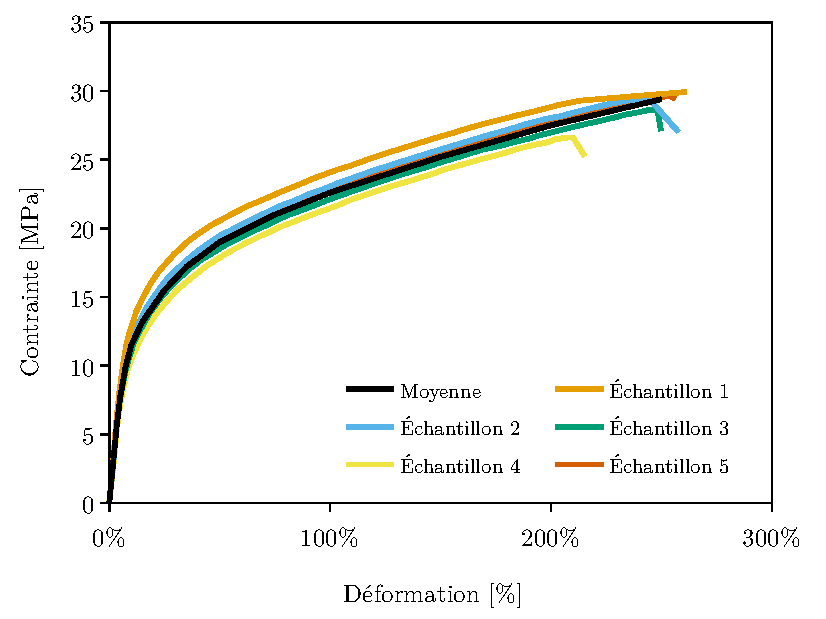
\includegraphics[width=0.7\textwidth]{STM1500_tension.pdf}
	\caption{Résultats des essais de traction pour le PEI-siloxane}
	\label{fig:STM1500_tension}
\end{figure}

\FloatBarrier
\subsection{Essais de soudage isotherme}
 
Les essais de soudage pour le PEI-siloxane ont débuté avec un essai dans une étuve sous vide. 
Un échantillon (Fig. \ref{fig:etuve_STM1500}) y a été inséré et chauffé jusqu'à \SI[locale=FR]{280}{\celsius} pendant 24 heures. 
À la sortie de l'étuve, l'échantillon était totalement plat (Fig. \ref{fig:etuve_STM1500_flat}), mais après avoir séparé le nanocomposite du composite, une portion de l'élastomère ne pouvait être retirée (Fig. \ref{fig:etuve_STM1500_adhesion}). 
En raison de la faible distance de diffusion des chaînes de polymère, même lors d'un soudage réussi, il a été impossible de confirmer au microscope optique ou même par analyse atomique au microscope électronique à balayage la diffusion des chaînes au travers de l'interface. 
Il est également possible de remarquer que durant cet essai, la couleur de l'élastomère a changé, avec une transition de sa teinte vers le brun.  
Ce dernier signe démontre un début de dégradation thermique de l'élastomère lors d'une exposition prolongée à des températures élevées. 
Il est important de vérifier qu'un procédé plus court ne produira pas de dégradation de l'élastomère. 
La prochaine étape de cette validation pour le PEI-siloxane était de produire une soudure dans une presse chauffante. 
À la fin de cet essai, encore une fois, en raison de la pression élevée, l'élastomère a presque totalement quitté la zone à souder (Fig. \ref{fig:welds_STM1500_presse}), mais après séparation des composants un film d'élastomère est resté fortement adhéré au nanocomposite (Fig. \ref{fig:welds_STm1500_presse_adhesion}). 
Cette fois par contre, le procédé, d'une durée d'approximativement \SI[locale=FR]{15}{\minute} en incluant le temps de refroidissement, a été assez rapide pour ne pas altérer de la couleur de l'élastomère. 

\begin{figure}[h]
	\centering
	\subfigure[]
	{\label{fig:weldstack_STm1500} 								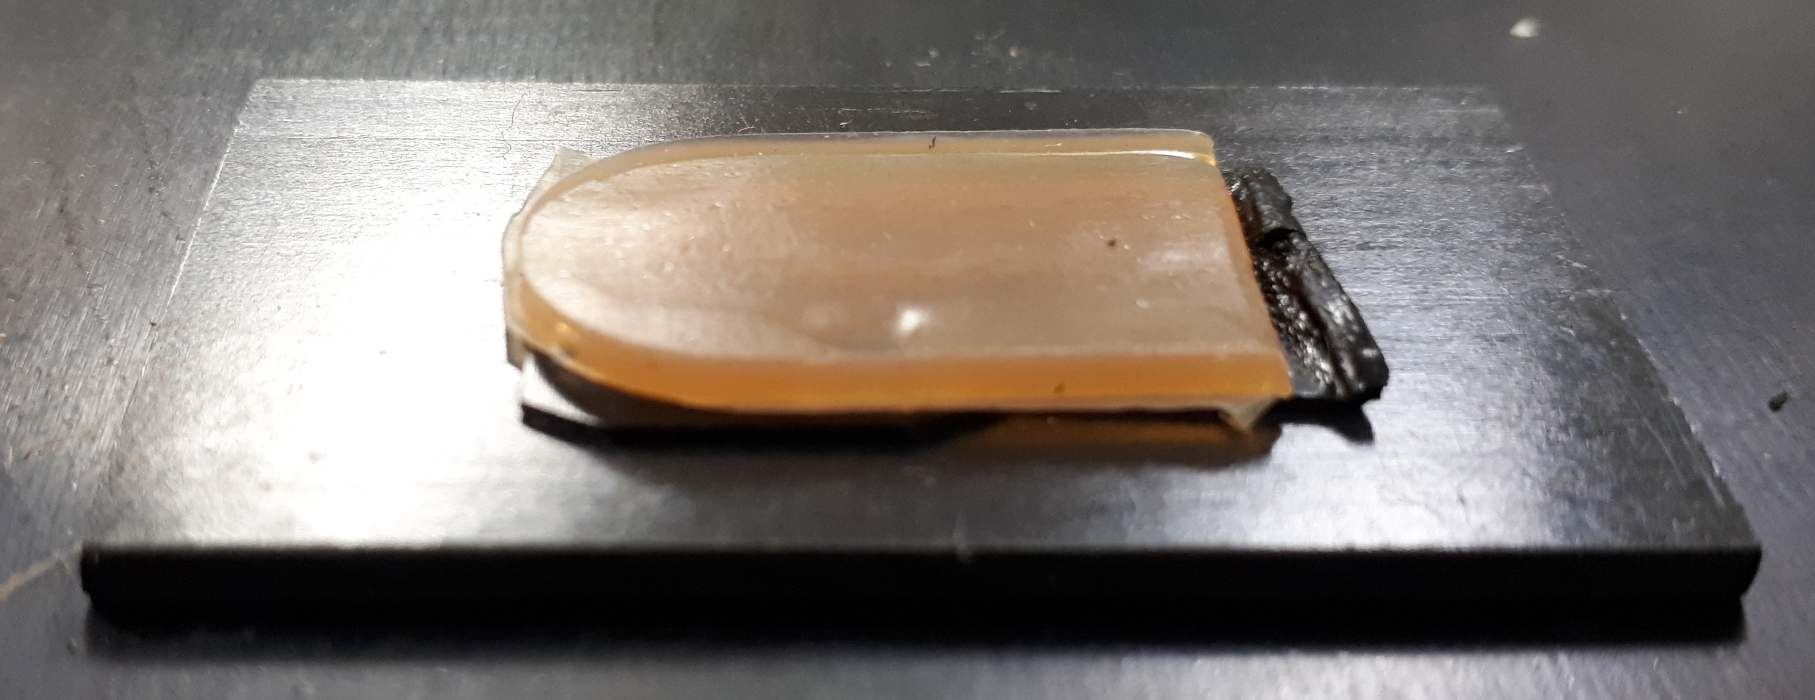
\includegraphics[height=3.6cm]{20181002_121017_crop_resize.jpg}	
	} \
	\subfigure[]
	{\label{fig:etuve_STM1500_flat} 								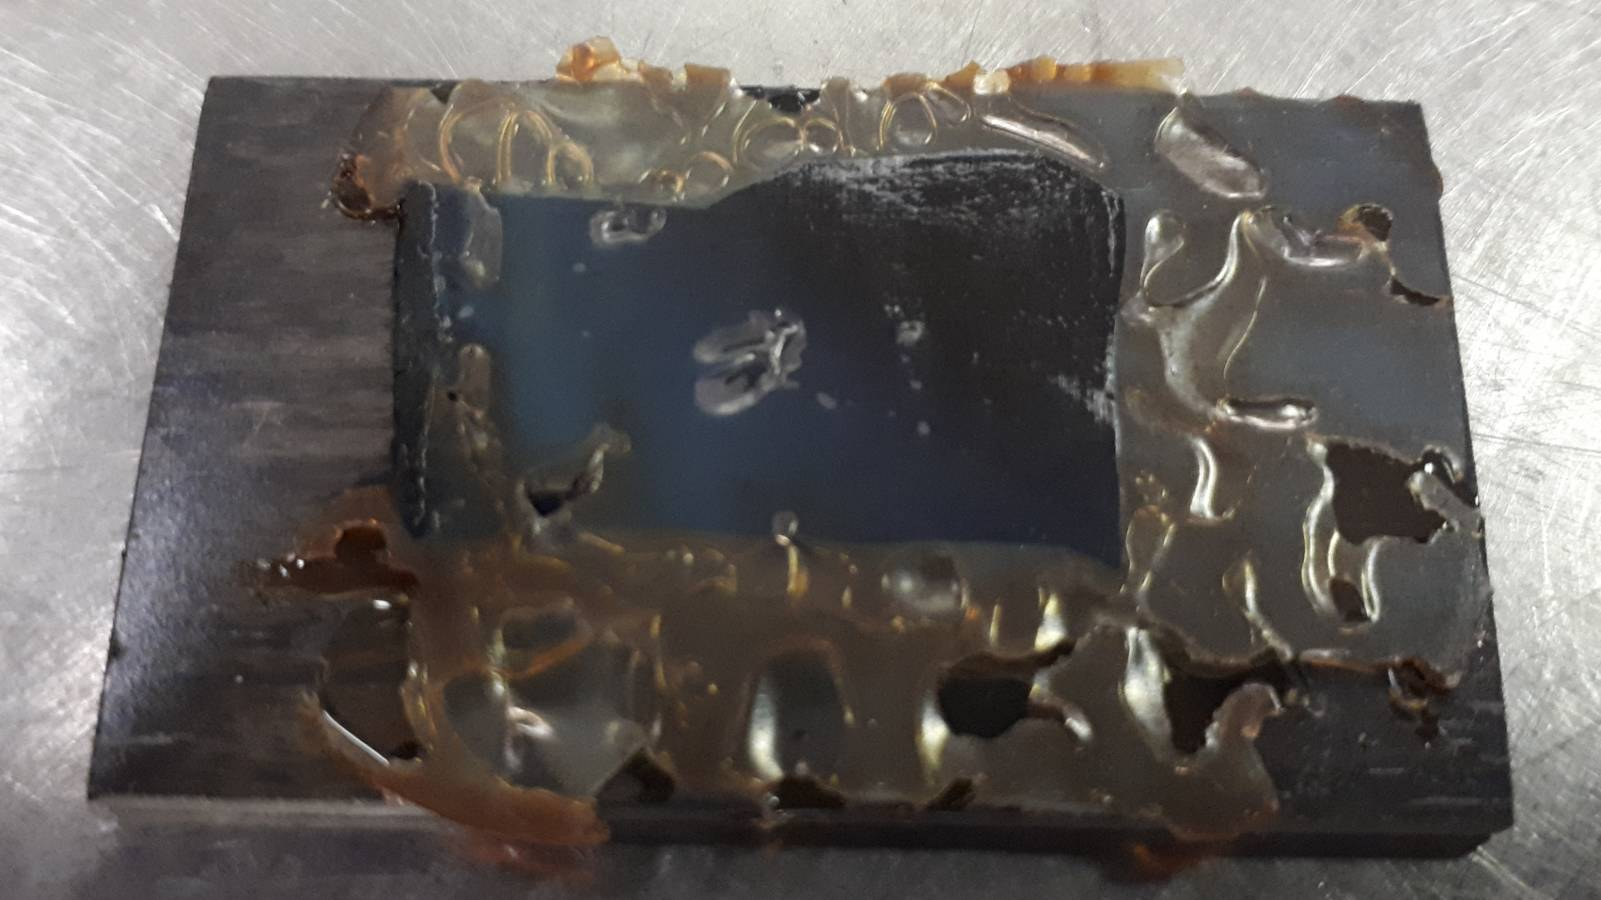
\includegraphics[height=3.6cm]{20181003_100733_crop_resize.jpg}
	} \
	\subfigure[]
	{\label{fig:etuve_STM1500_adhesion}
		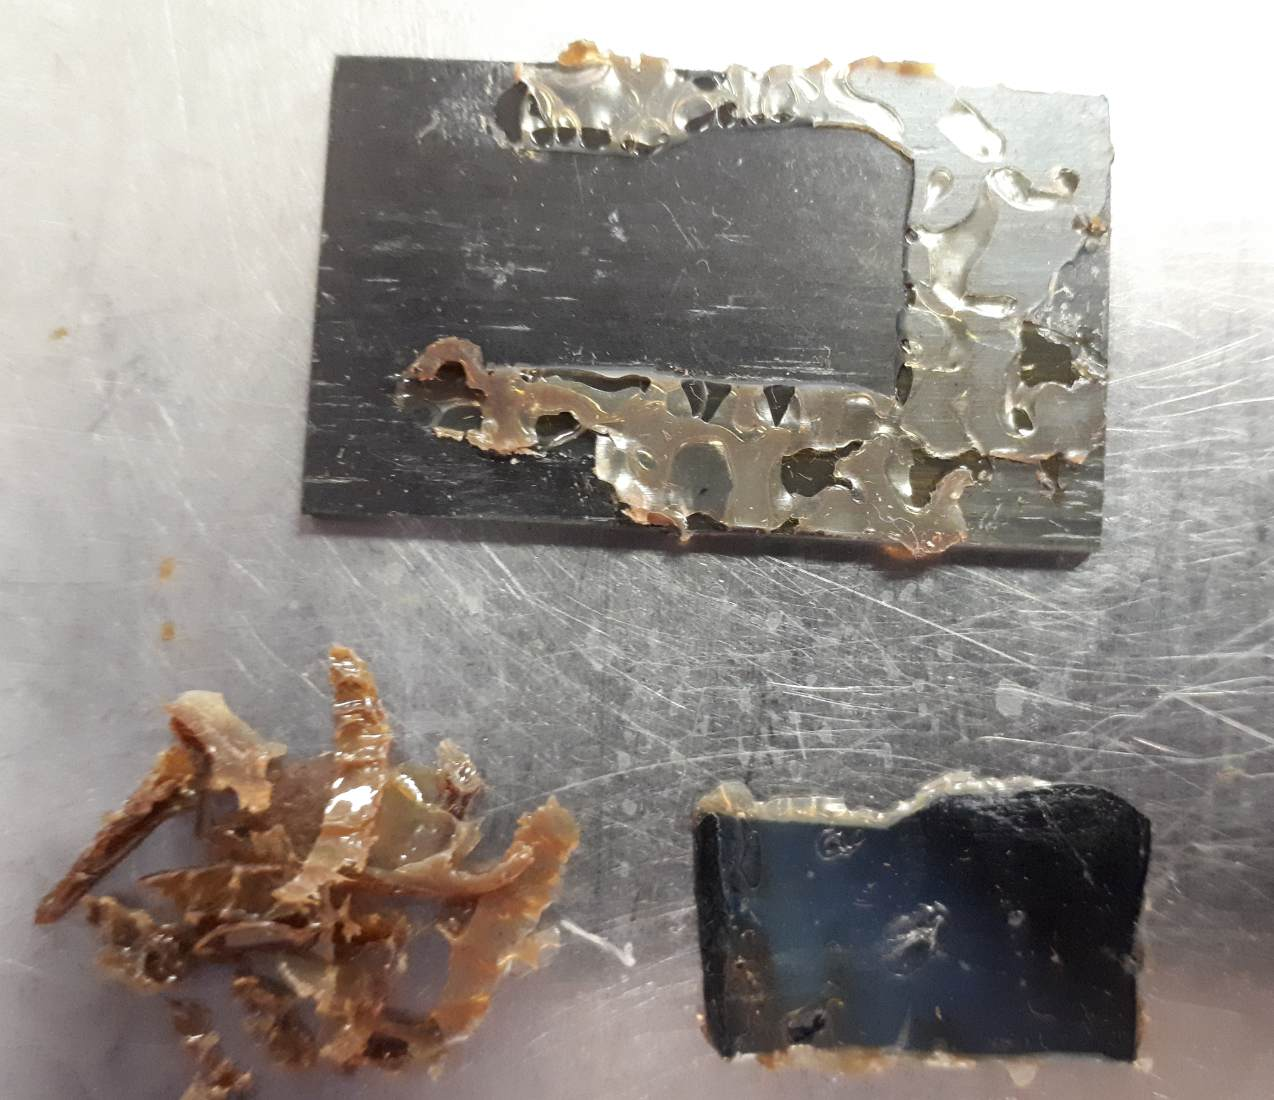
\includegraphics[height=3.6cm]{20181003_102113_crop_resize.jpg}
	}
	\caption{Essai de soudage dans une étuve sous vide à \SI{280}{\celsius} pour l'élastomère PEI-siloxane présentant a) la préparation de l'échantillons, b) l'échantillon à la sortie de l'étuve et c) l'adhésion de l'élastomère sur le nanocomposite}
	\label{fig:etuve_STM1500}

	\centering
	\subfigure[]
	{\label{fig:welds_STM1500_presse} 								
		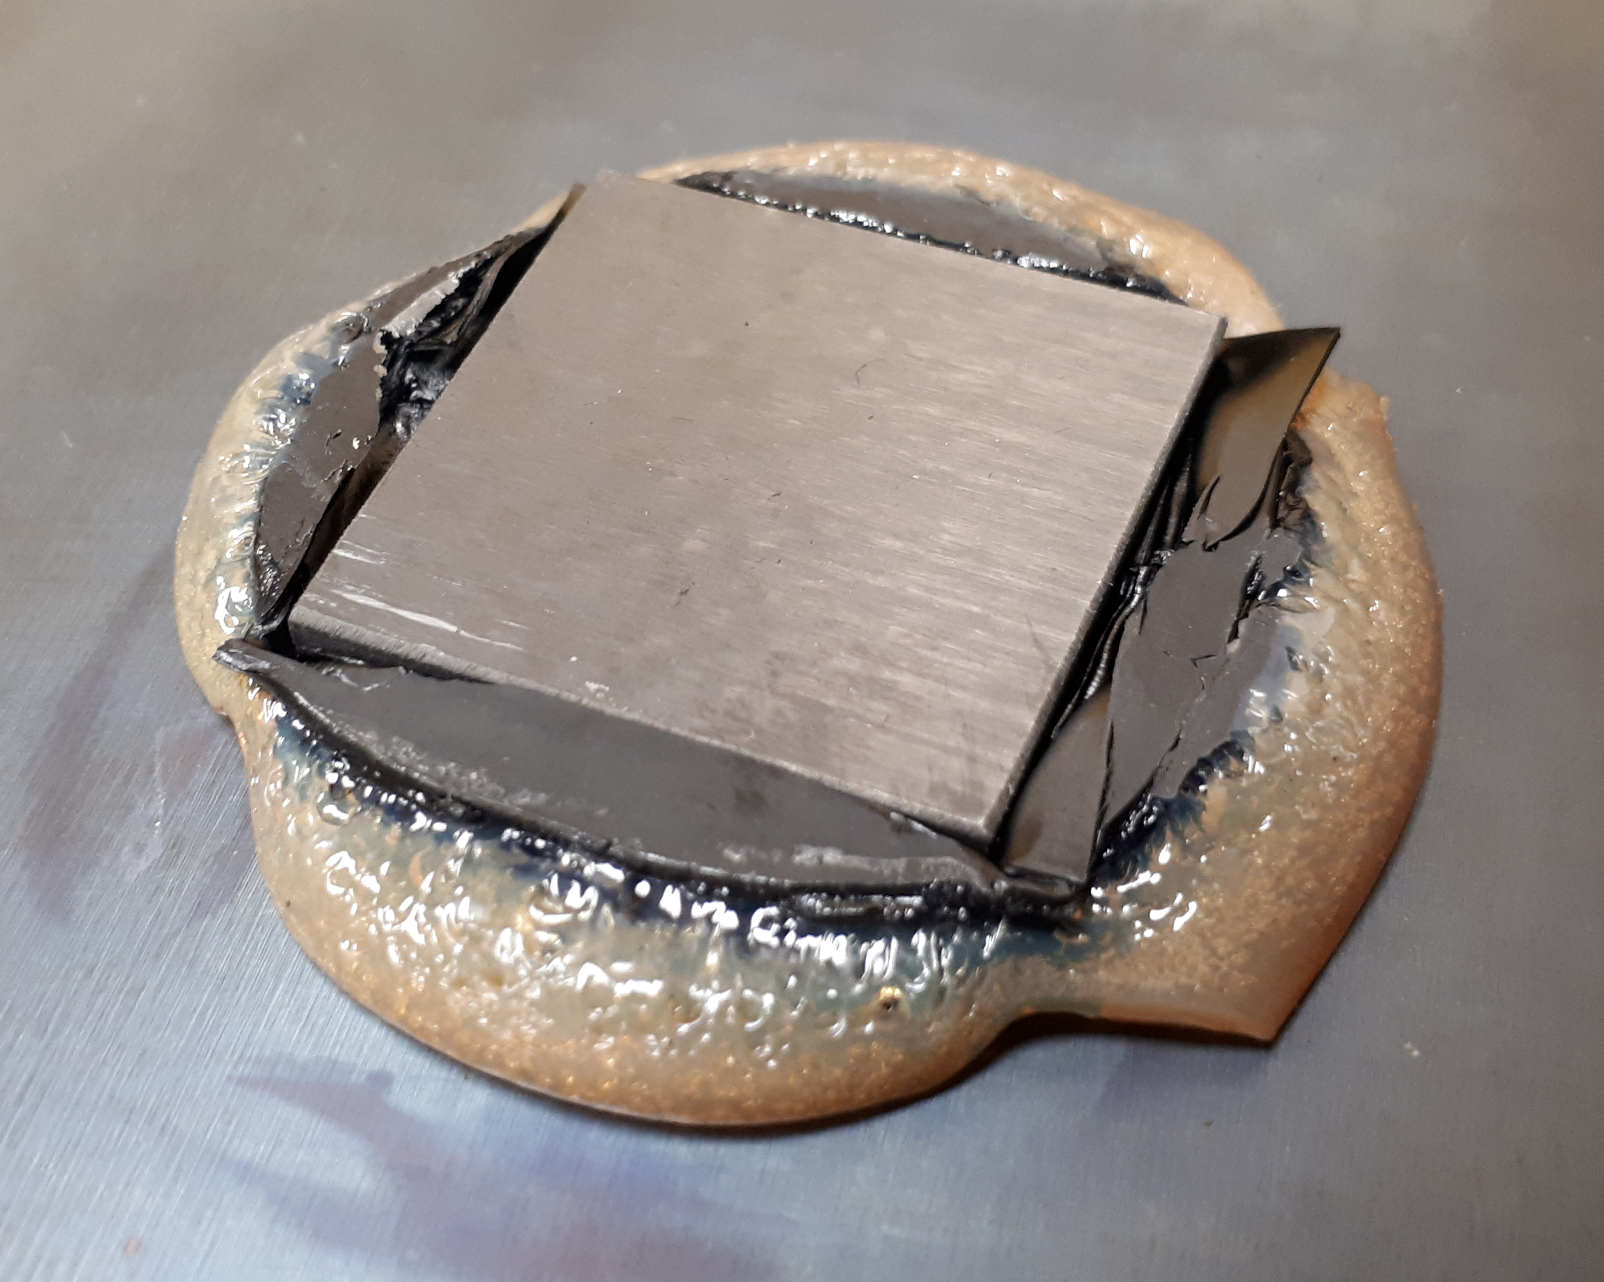
\includegraphics[height=4.5cm]{20181108_100951_crop_resize.jpg}
	} \qquad
	\subfigure[]
	{\label{fig:welds_STm1500_presse_adhesion} 								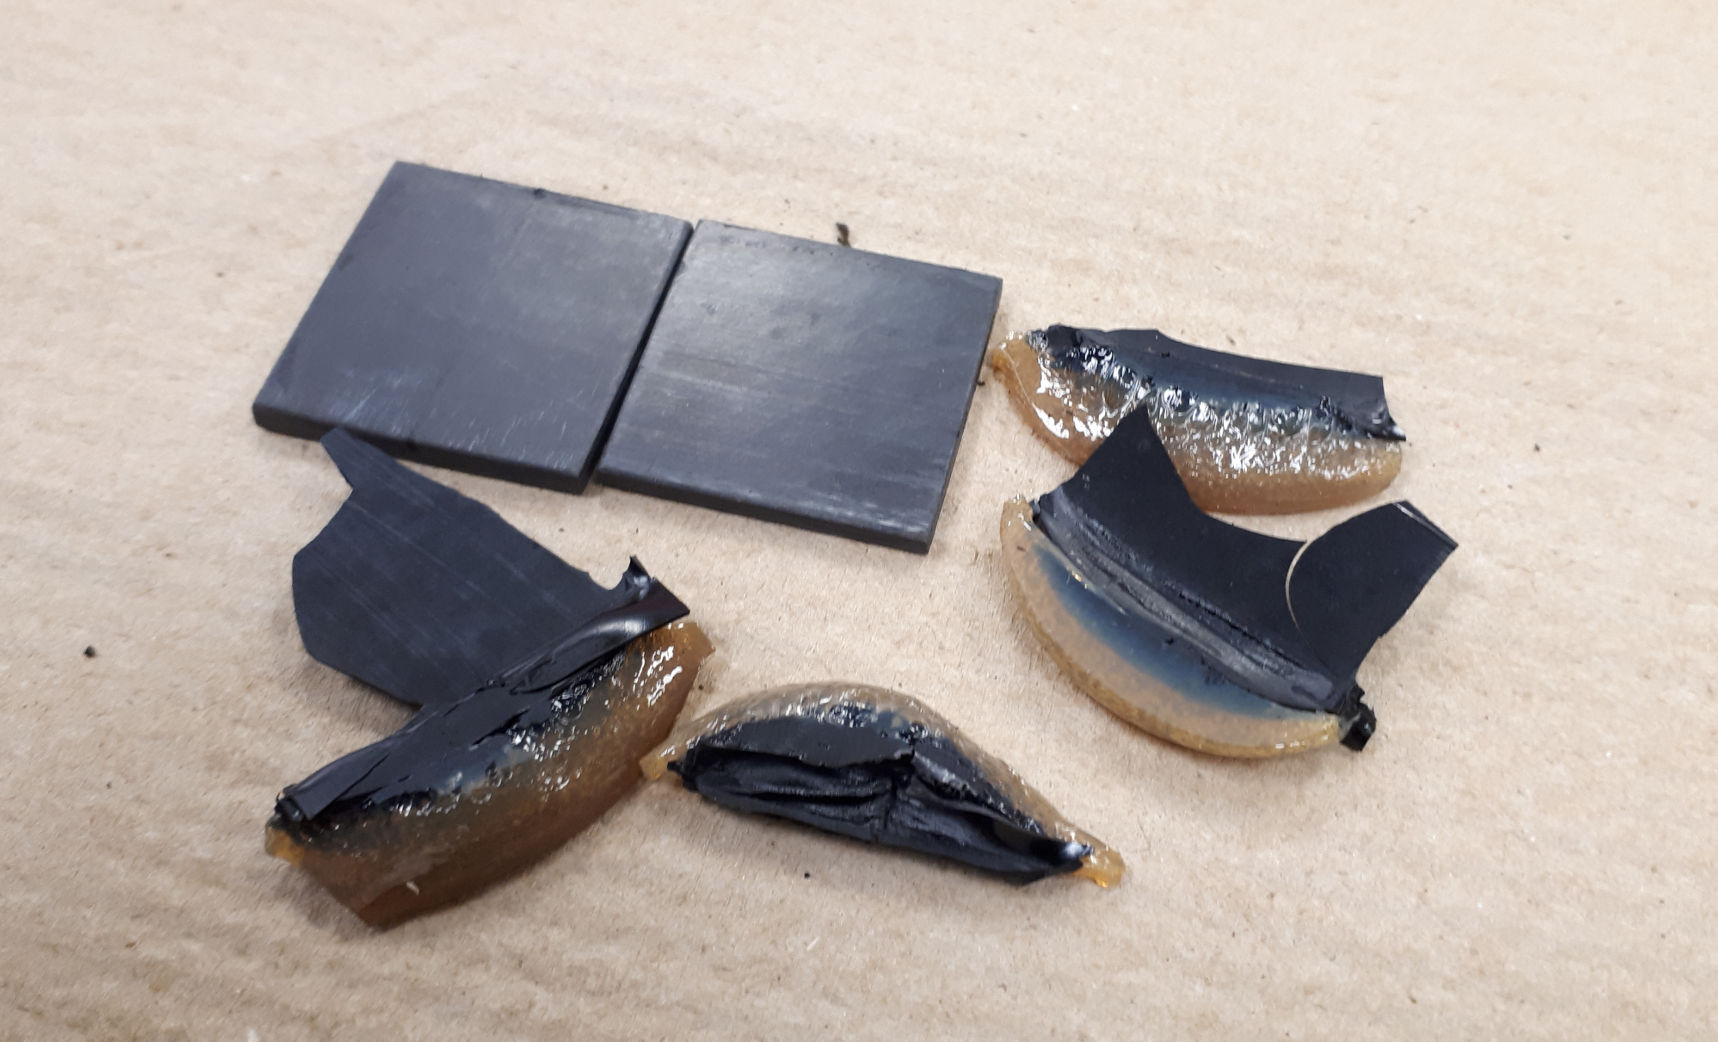
\includegraphics[height=4.5cm]{20181108_101250_resize_crop.jpg}
	}
	\caption{Essai de soudage à la presse à \SI{280}{\celsius} pour l'élastomère PEI-siloxane présentant a) l'échantillon à la sortie de la presse et b) l'adhésion de l'élastomère sur le nanocomposite}
	\label{fig:presse_STM1500}
\end{figure}

Un point intéressant à noter est que malgré l'adhésion visible entre l'élastomère et le nanocomposite, le soudage entre le composite et le nanocomposite n'arrive pas à se produire aux températures employées lors des essais à l'étuve ou dans la presse. 
Ce comportement peut être lié à la quantité de charges dans le nanocomposite qui en viennent à affecter la mobilité des chaînes de polymère. 
Ce même comportement avait été dénoté dans le chapitre \ref{sec:Theme2} et causait une augmentation de la température nécessaire pour le soudage. 
Cet indice porte à croire que les températures d'opération pour les deux types de soudage ne seront pas nécessairement compatibles. 

\FloatBarrier

\subsection{Évaluation de la vitesse de dégradation thermique du PEI-siloxane}

Afin de déterminer un temps maximal pour le soudage, il est nécessaire d'évaluer plus précisément la vitesse de dégradation thermique du PEI-siloxane. 
Un mélange composé de PEI et 10\% d'élastomère a été produit. 
Lors de ce test, le PEI a été mélangé avec une vitesse de rotation de 150 RPM jusqu'à ce que la température du mélange se stabilise à \SI[locale=FR]{350}{\celsius}. 
Les granules de PEI-siloxane ont alors été ajoutées et le couple du rotor a été enregistré en continu pendant 40 minutes (Fig. \ref{fig:STM1500_thermo_Haake_couple}). 
On peut voir qu'après une fonte rapide, le couple remonte progressivement pour atteindre un plateau avec une légère pente aux alentours de \SI[locale=FR]{600}{\second} (10 minutes). 
Ce plateau se poursuit pendant 15 minutes jusqu'à approximativement \SI[locale=FR]{1500}{\second} (25 minutes) avant que la viscosité ne commence à augmenter de plus en plus rapidement. 
L'élastomère recueilli après cet essai présentait des signes flagrants de dégradation thermique (Fig. \ref{fig:STM1500_thermo_Haake_degradation}). 
Ces résultats permettent de confirmer que la stabilité thermique du PEI-siloxane est suffisante pour réaliser des soudures à condition que la température soit gardée sous contrôle. 

\begin{figure}[h]	
	\centering
	\subfigure[]
	{\label{fig:STM1500_thermo_Haake_couple} 								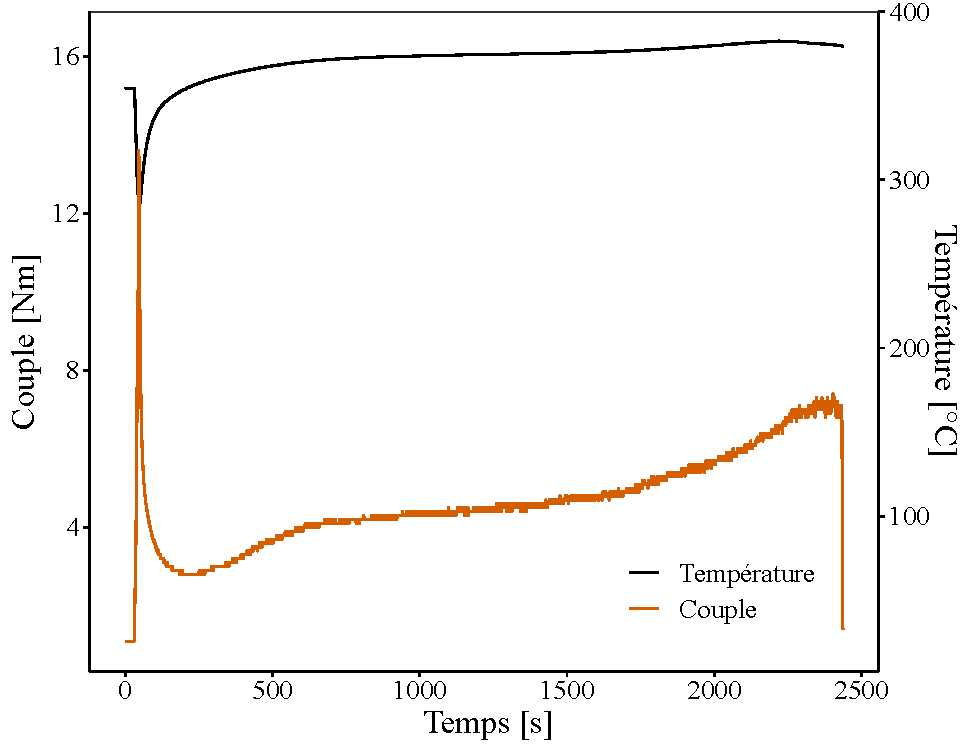
\includegraphics[height=7cm]{thermo_haake_STM1500.pdf}
	} \qquad
	\subfigure[]
	{\label{fig:STM1500_thermo_Haake_degradation}
		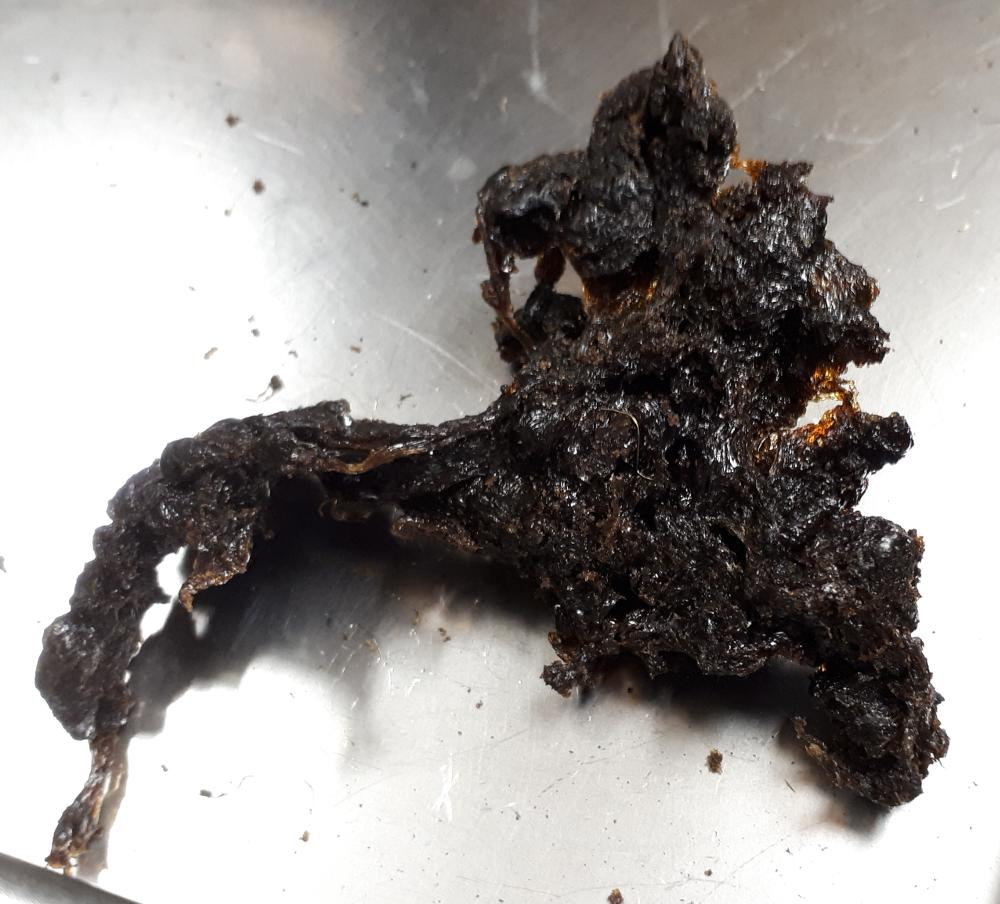
\includegraphics[height=5.cm]{20190822_110329_crop_resize.jpg}
	} \\
	\caption{Évaluation de la stabilité thermique du PEI-siloxane à l'aide d'un mélangeur interne présentant a) l'évolution du couple pendant le mélange et b) l'état de dégradation de l'élastomère après 40 minutes}
	\label{fig:STM1500_thermo_Haake}
\end{figure}

Une analyse des mécanismes de dégradation serait nécessaire pour expliquer les raisons menant à la variation de couple lors de cet essai. 
Il n'a pas été possible de trouver de telles analyses dans la littérature pour le PEI-siloxane. 
Par contre, en ce qui concerne le siloxane, la dégradation de ce polymère produit des groupe cycliques de siloxane qui réduisent l'élasticité \cite{Heinemann2004}. 
Ce mécanisme pourrait expliquer une partie du comportement observé.  

\FloatBarrier

\subsection{Essais de soudage par résistance}

Un premier essai a été réalisé dans le montage de soudage par résistance à l'aide de petits échantillons d'élastomère et de composite ainsi qu'un élément chauffant nanocomposite. 
L'échantillon a été installé dans le montage de soudage (Fig. \ref{fig:STM1500_soudure_montage}) et un essai de soudage a été réalisé avec une puissance surfacique de \SI[locale=FR]{260}{\kilo\watt\per\square\metre} pendant \SI[locale=FR]{60}{\second}. 
Une jonction a été obtenue en une seule étape lors de cet essai. 
Les tentatives pour séparer l'élastomère ont, encore une fois, permis de séparer le nanocomposite du composite, mais sans permettre de séparer l'élastomère du nanocomposite. 
En raison de l'absence de soudure entre les adhérents composites et les éléments chauffants nanocomposites, la méthode de soudure en une étape a été abandonnée.
Les essais subséquents ont utilisé un mode de soudure en deux étapes où l'élément chauffant était préalablement soudé sur un adhérent composite. 

\FloatBarrier
\begin{figure}[h]
	\centering
	\subfigure[]
	{\label{fig:STM1500_soudure_montage} 								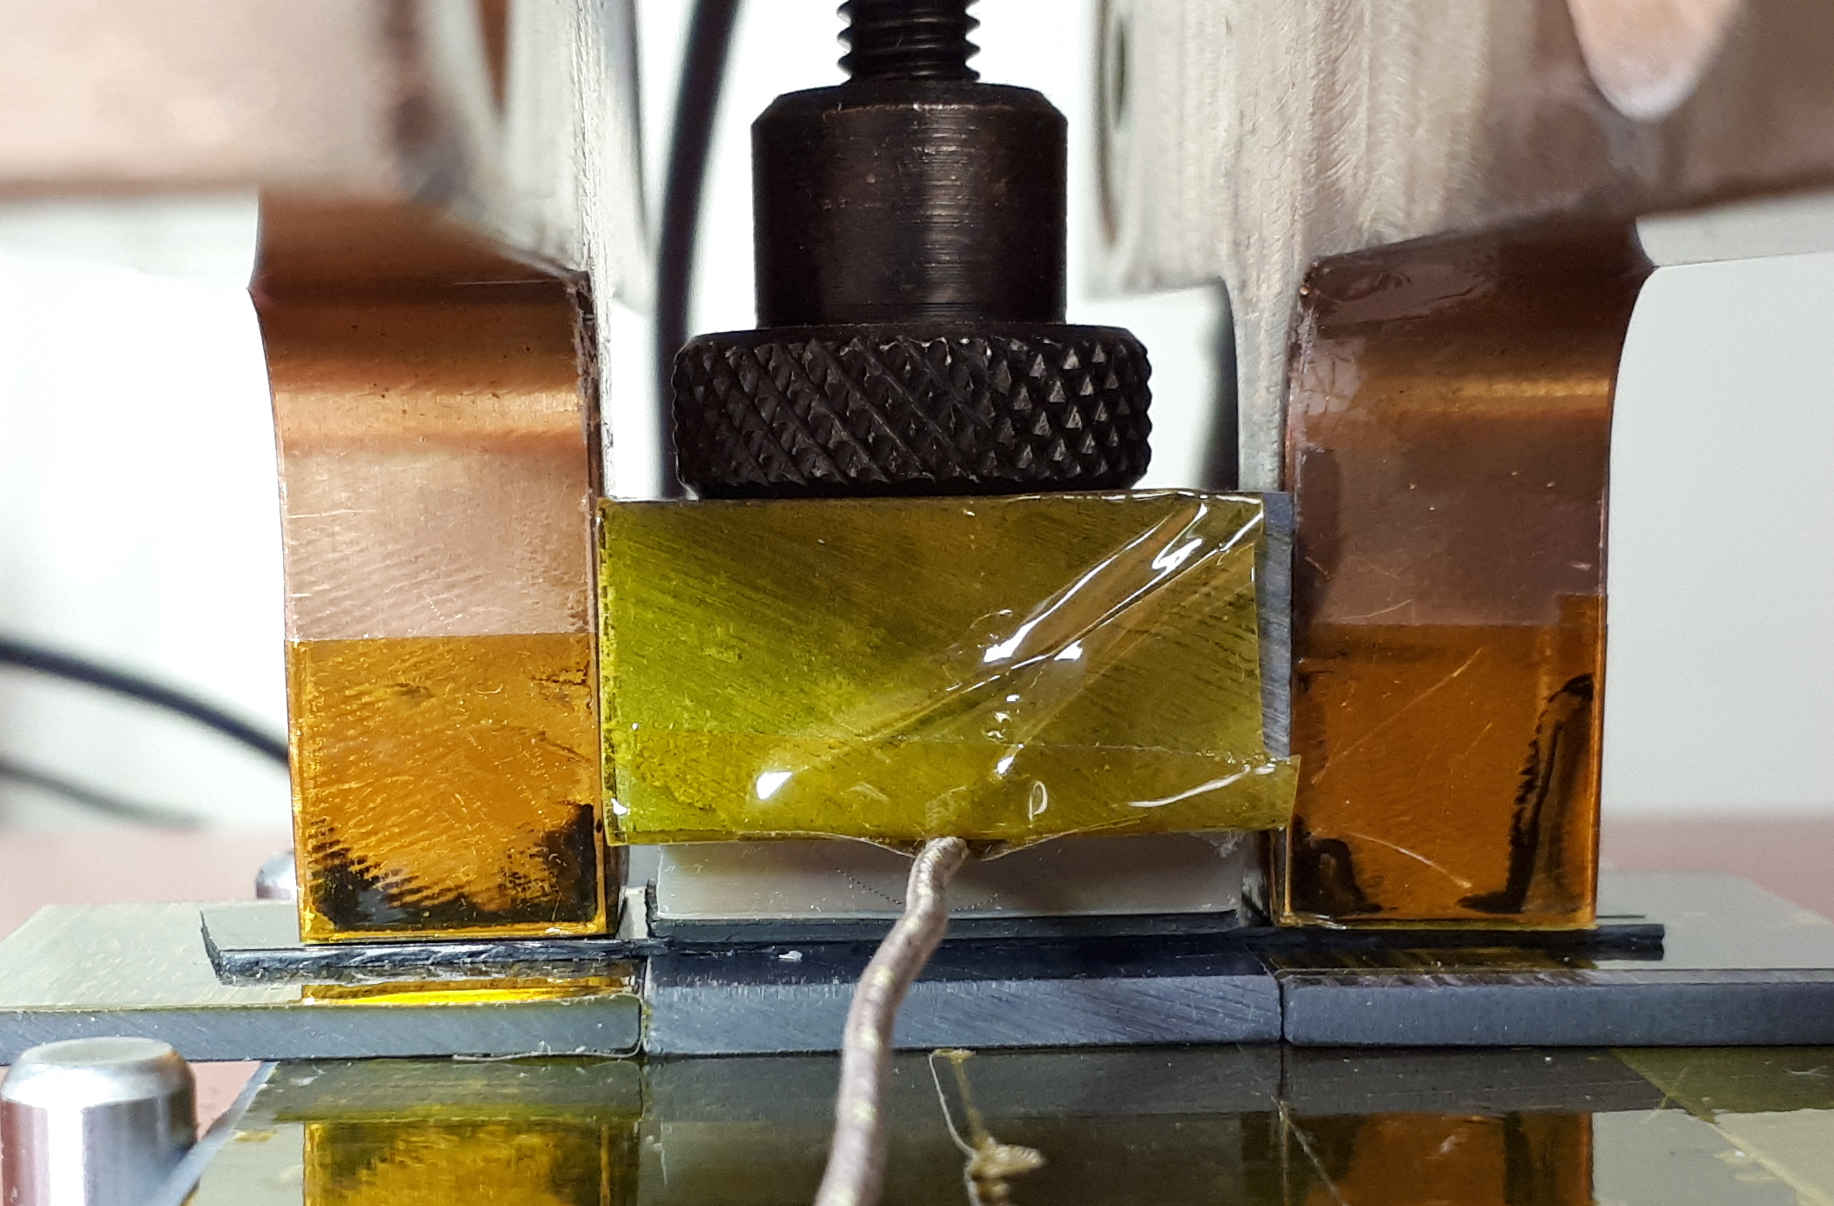
\includegraphics[height=4.25cm]{20181109_111133_crop_resize.jpg}
	} \qquad
	\subfigure[]
	{\label{fig:STM1500_soudure_resultat}
		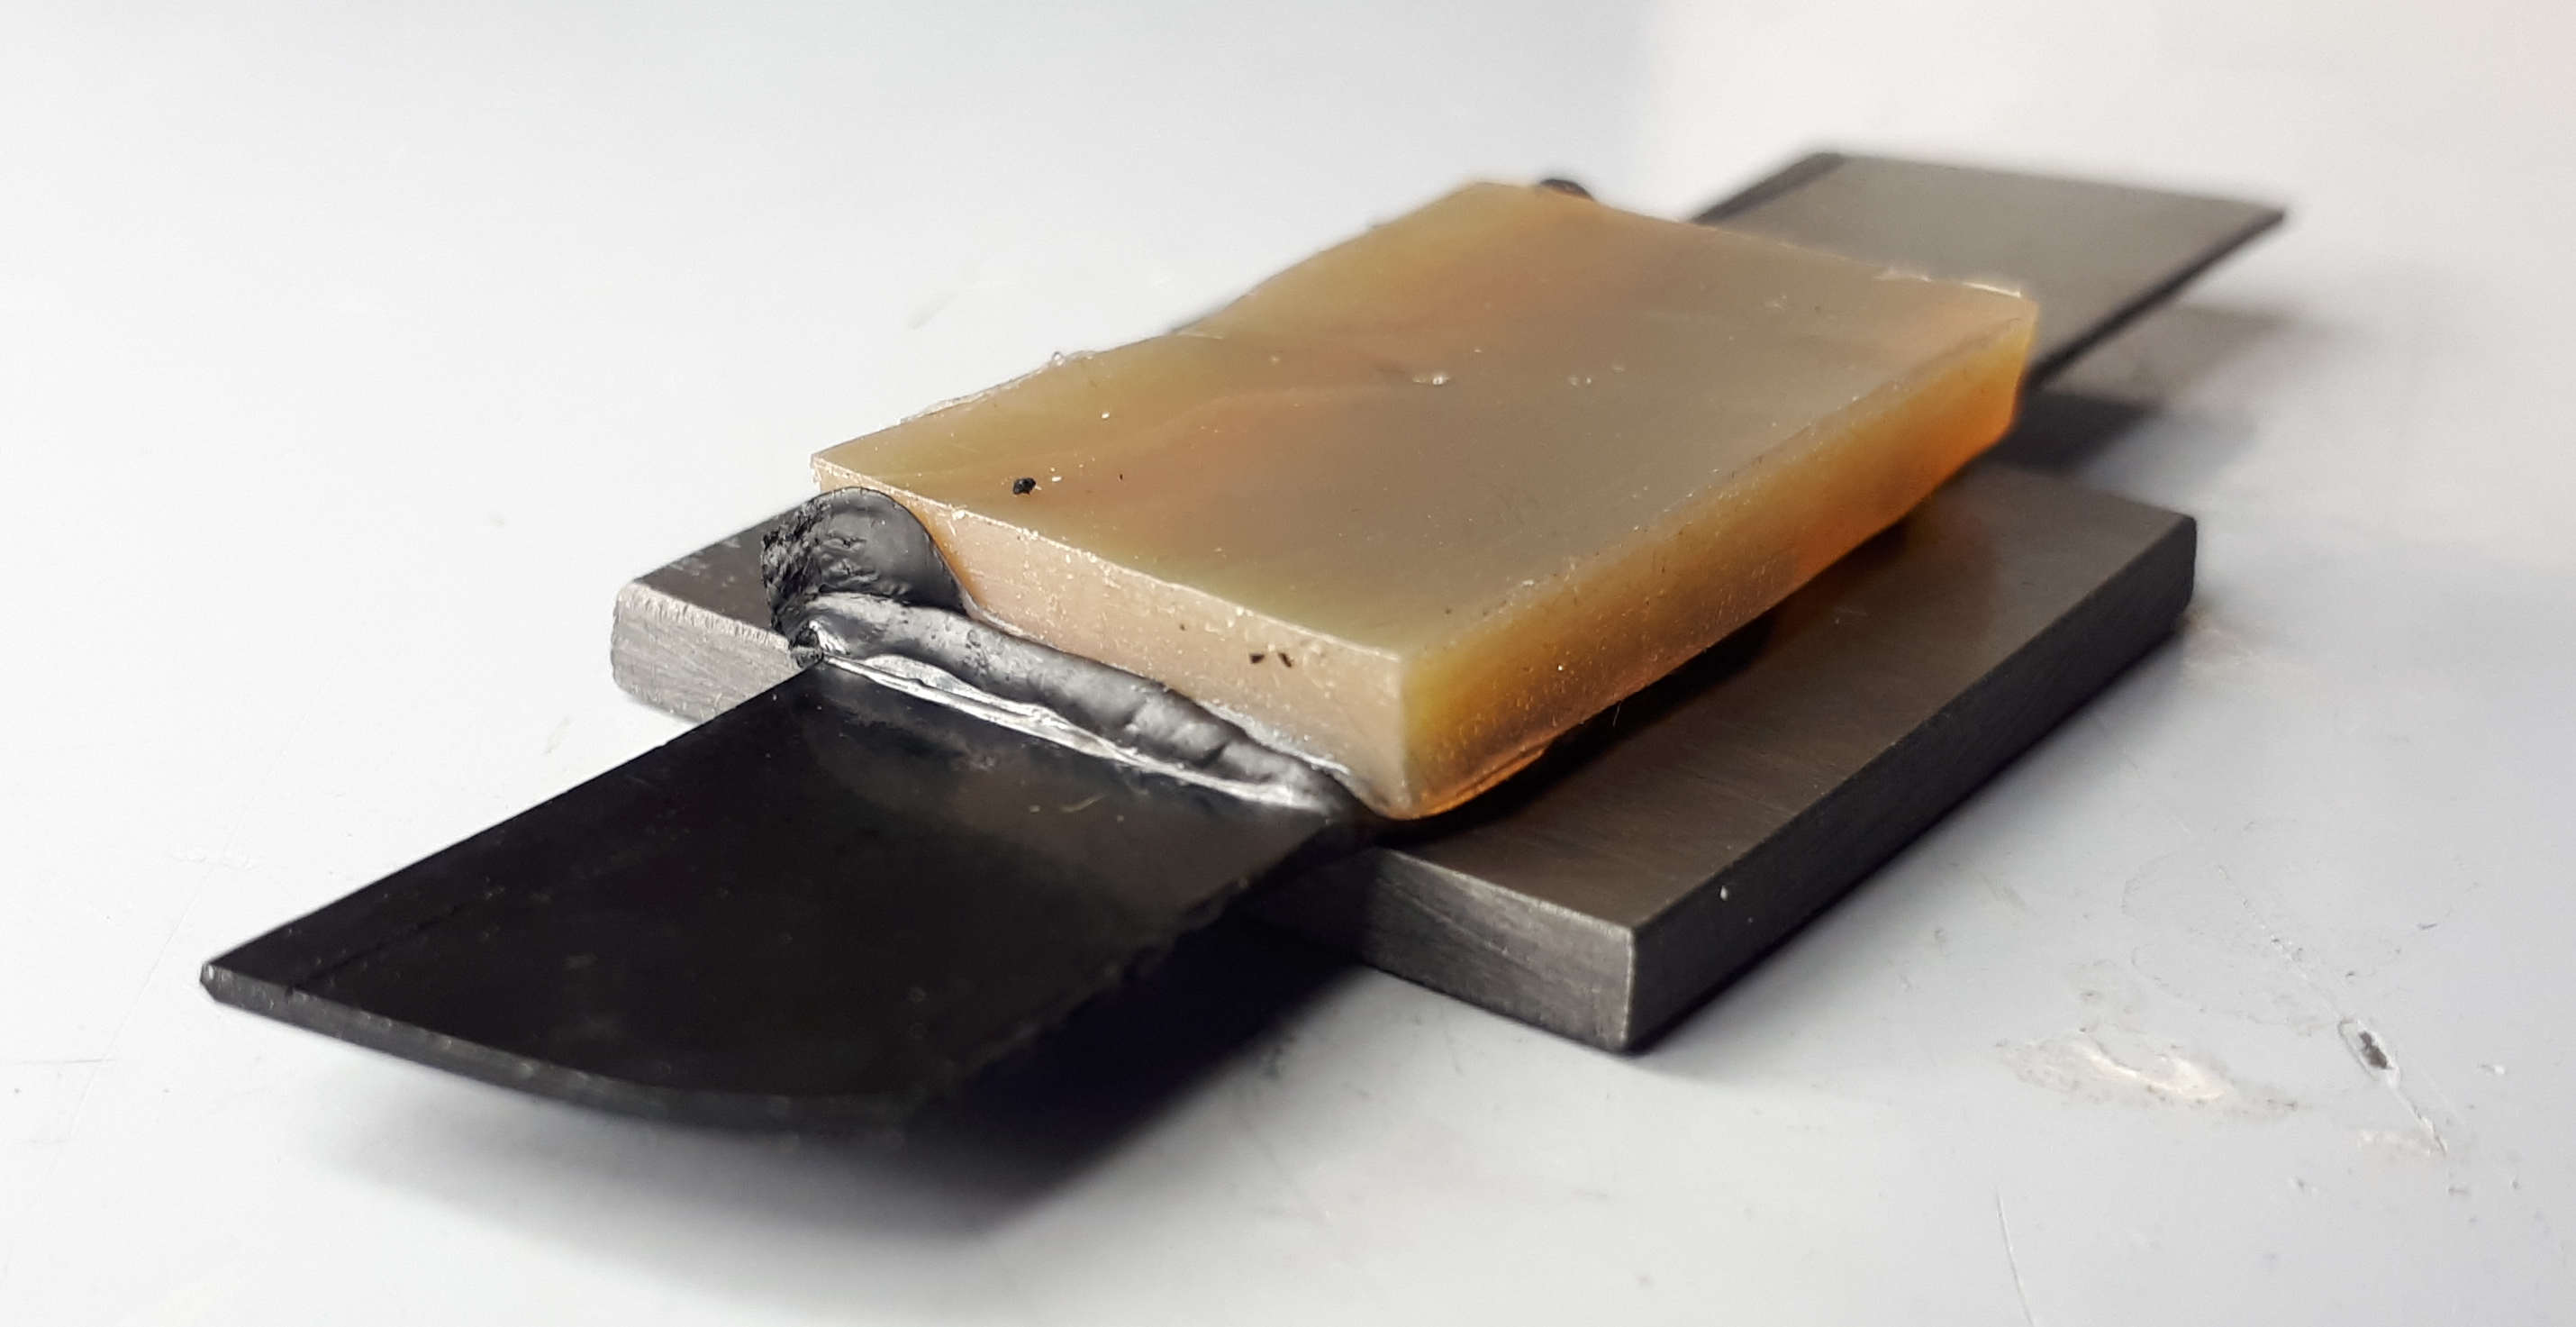
\includegraphics[height=4.25cm]{20181109_113850_crop.jpg}
	}
	\caption{Essai de soudage d'un échantillon avec l'élastomère PEI-siloxane avec a) l'échantillon positionné dans le montage de soudage et b) le résultat de l'essai de soudage}
	\label{fig:STM1500_soudure}
\end{figure}
\FloatBarrier

Une série de soudures exploratoires ont été réalisées afin de cerner une fenêtre d'opération. 
Lors des essais initiaux, des thermocouples étaient installés pour mesurer l'élévation de température sur la face opposée de l'élastomère. 
Les essais étaient arrêtés si la température s'élevait rapidement au-dessus des températures pouvant causer une dégradation rapide de l'élastomère ou un fluage prononcé de l'élastomère en dehors de la zone soudée. 
Les deux premiers essais à 260 et \SI[locale=FR]{220}{\kilo\watt\per\square\metre} ont dû être arrêtés après seulement \SI[locale=FR]{60}{\second} en raison de dégagements de fumée (Fig. \ref{fig:MM_260_60} et \ref{fig:MM_220_60}). 
Dans les deux cas, l'élastomère a pu être facilement arraché de la jonction après la soudure et on pouvait voir des signes de dégradation de l'élastomère et du nanocomposite. 
Il était alors nécessaire de considérer alors deux options, souder à plus faible puissance pendant un temps prolongé ou souder brièvement à haute puissance. 
Le troisième essai a été réalisé à une plus faible puissance de \SI[locale=FR]{180}{\kilo\watt\per\square\metre} pendant \SI[locale=FR]{180}{\second} (Fig. \ref{fig:MM_180_180}). 
L'essai a été arrêté lorsque la face supérieure a atteint la température de \SI[locale=FR]{120}{\celsius}. 
Pour cet échantillon, il a été possible de séparer aisément l'élastomère du nanocomposite et aucun signe de diffusion n'a été noté. 
Finalement pour l'approche avec un temps court et une puissance élevée, un échantillon a été produit avec une puissance surfacique de \SI[locale=FR]{300}{\kilo\watt\per\square\metre} et un temps de \SI[locale=FR]{45}{\second}. 
La rupture de l'élastomère pour cet essai s'est produite dans l'adhérent et une portion de l'élastomère est resté adhéré. 
Cette dernière condition de test a été répétée avec des adhérents sur des substrats métalliques. 
Les essais subséquents ont également utilisé des conditions similaires. 

\FloatBarrier
\begin{figure}[h]
	\centering
	\subfigure[]
	{\label{fig:MM_260_60} 								
		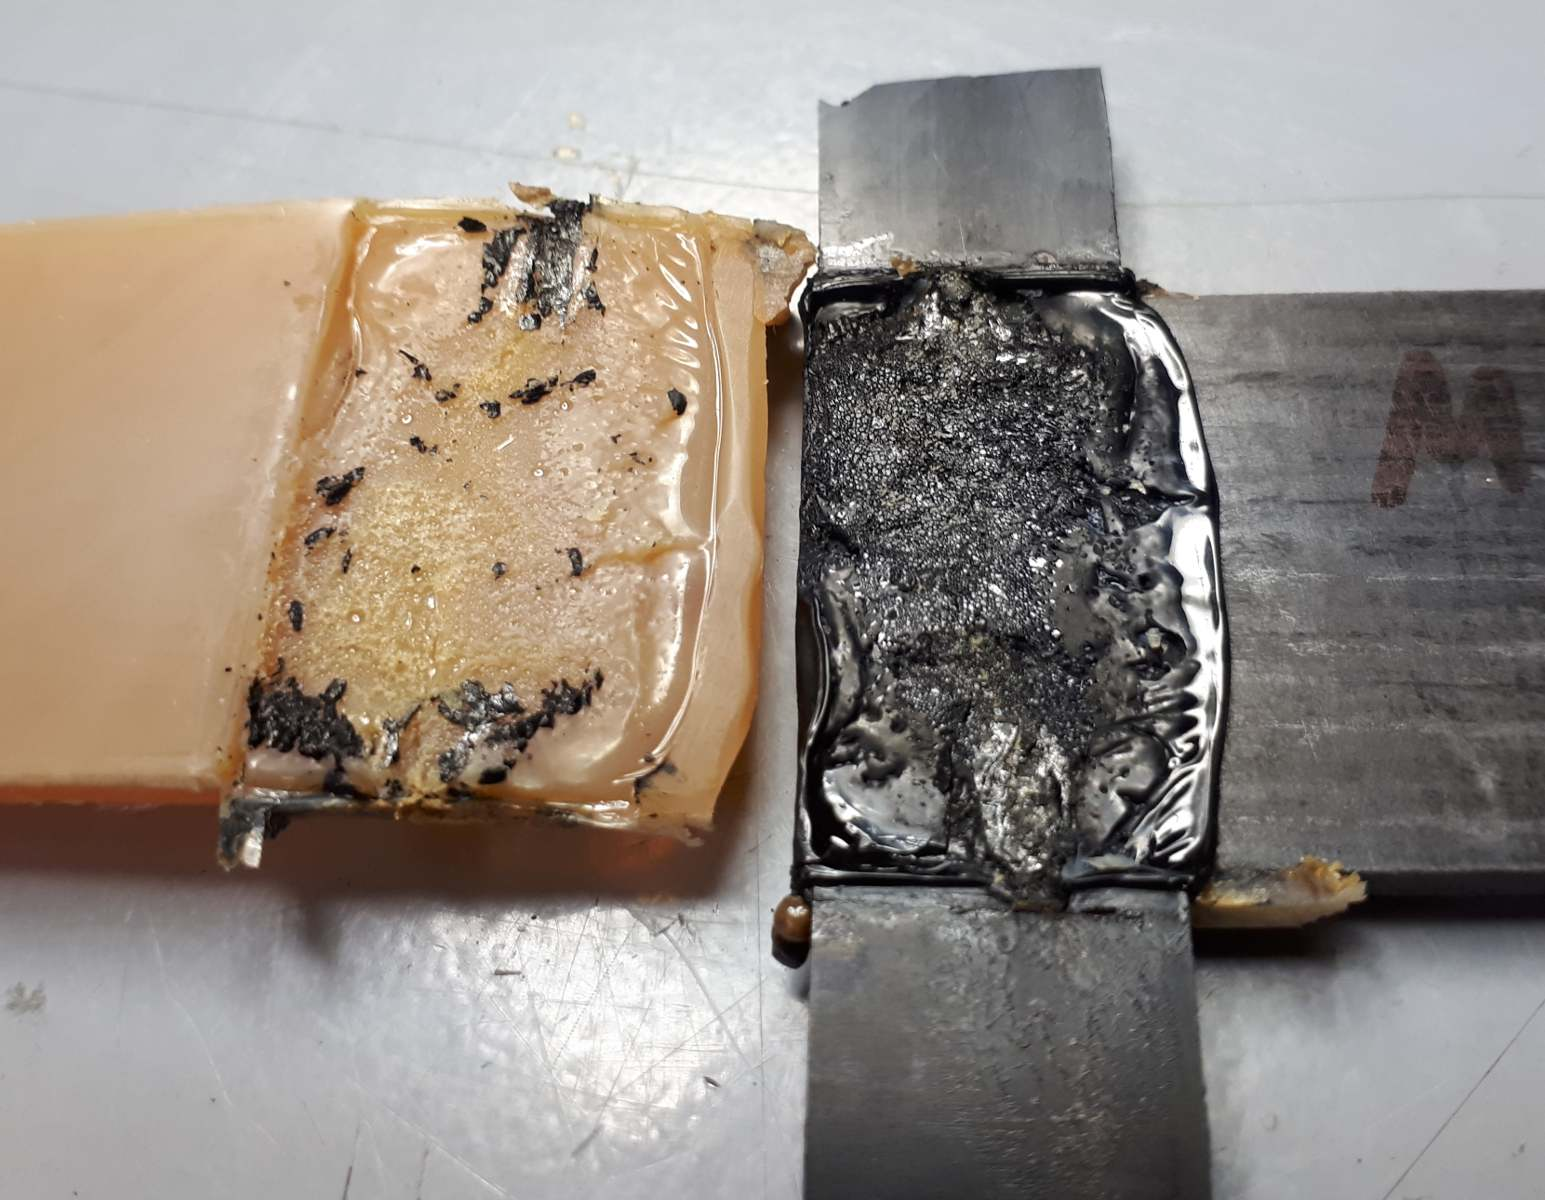
\includegraphics[height=5.5cm]{MM_260_60_crop_resize.jpg}
	} \qquad
	\subfigure[]
	{\label{fig:MM_220_60}
		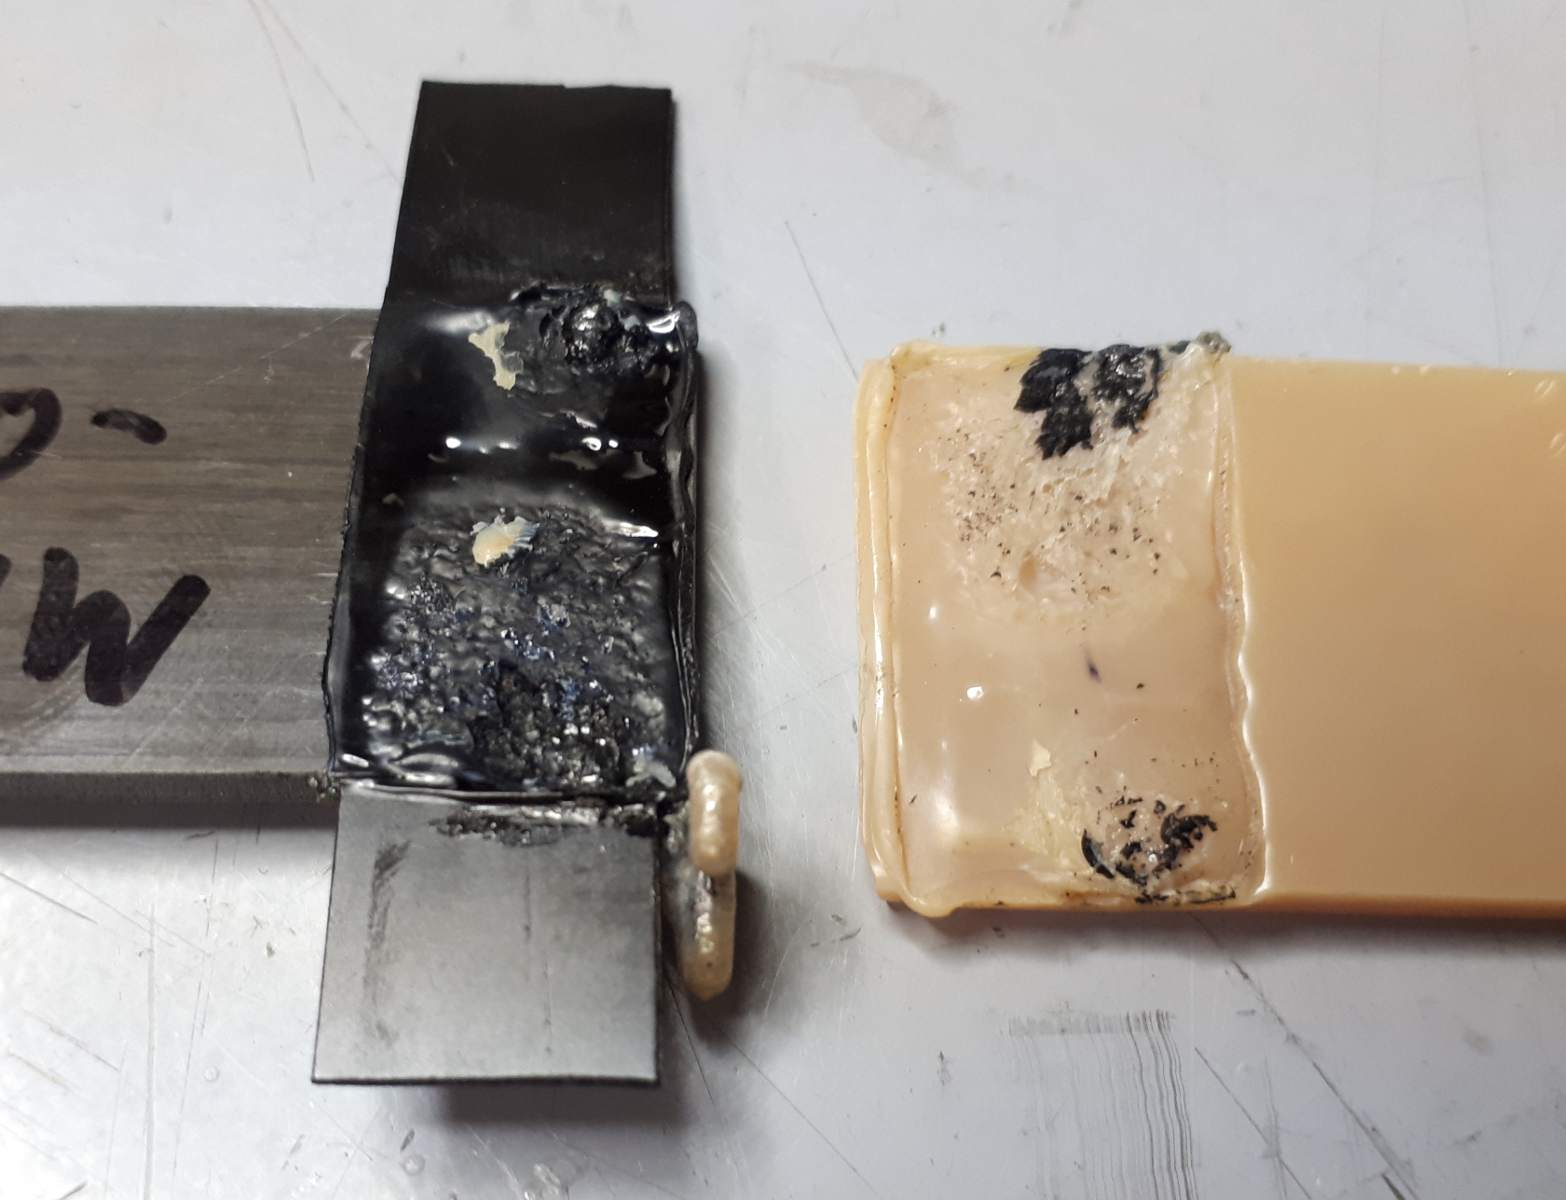
\includegraphics[height=5.5cm]{MM_220_60_crop_resize.jpg}
	} \\
	
	\subfigure[]
	{\label{fig:MM_180_180} 		
		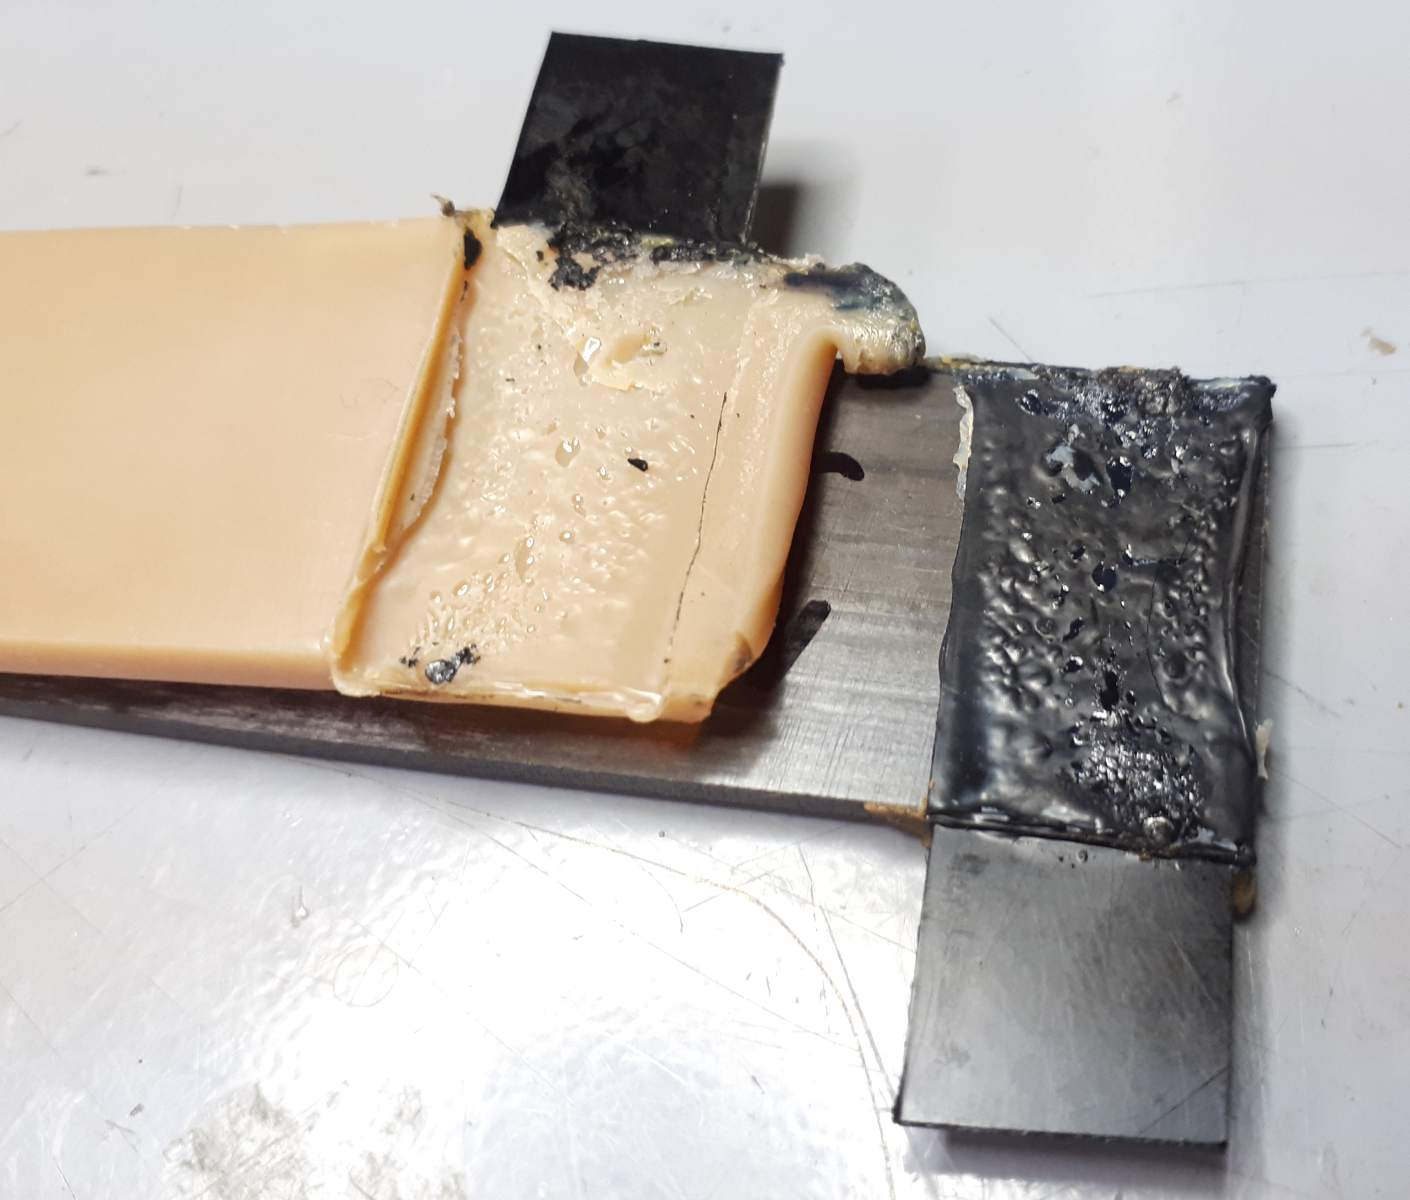
\includegraphics[height=5.5cm]{MM_180_180_crop_resize.jpg}
	} \qquad
	\subfigure[]
	{\label{fig:MM_300_45}
		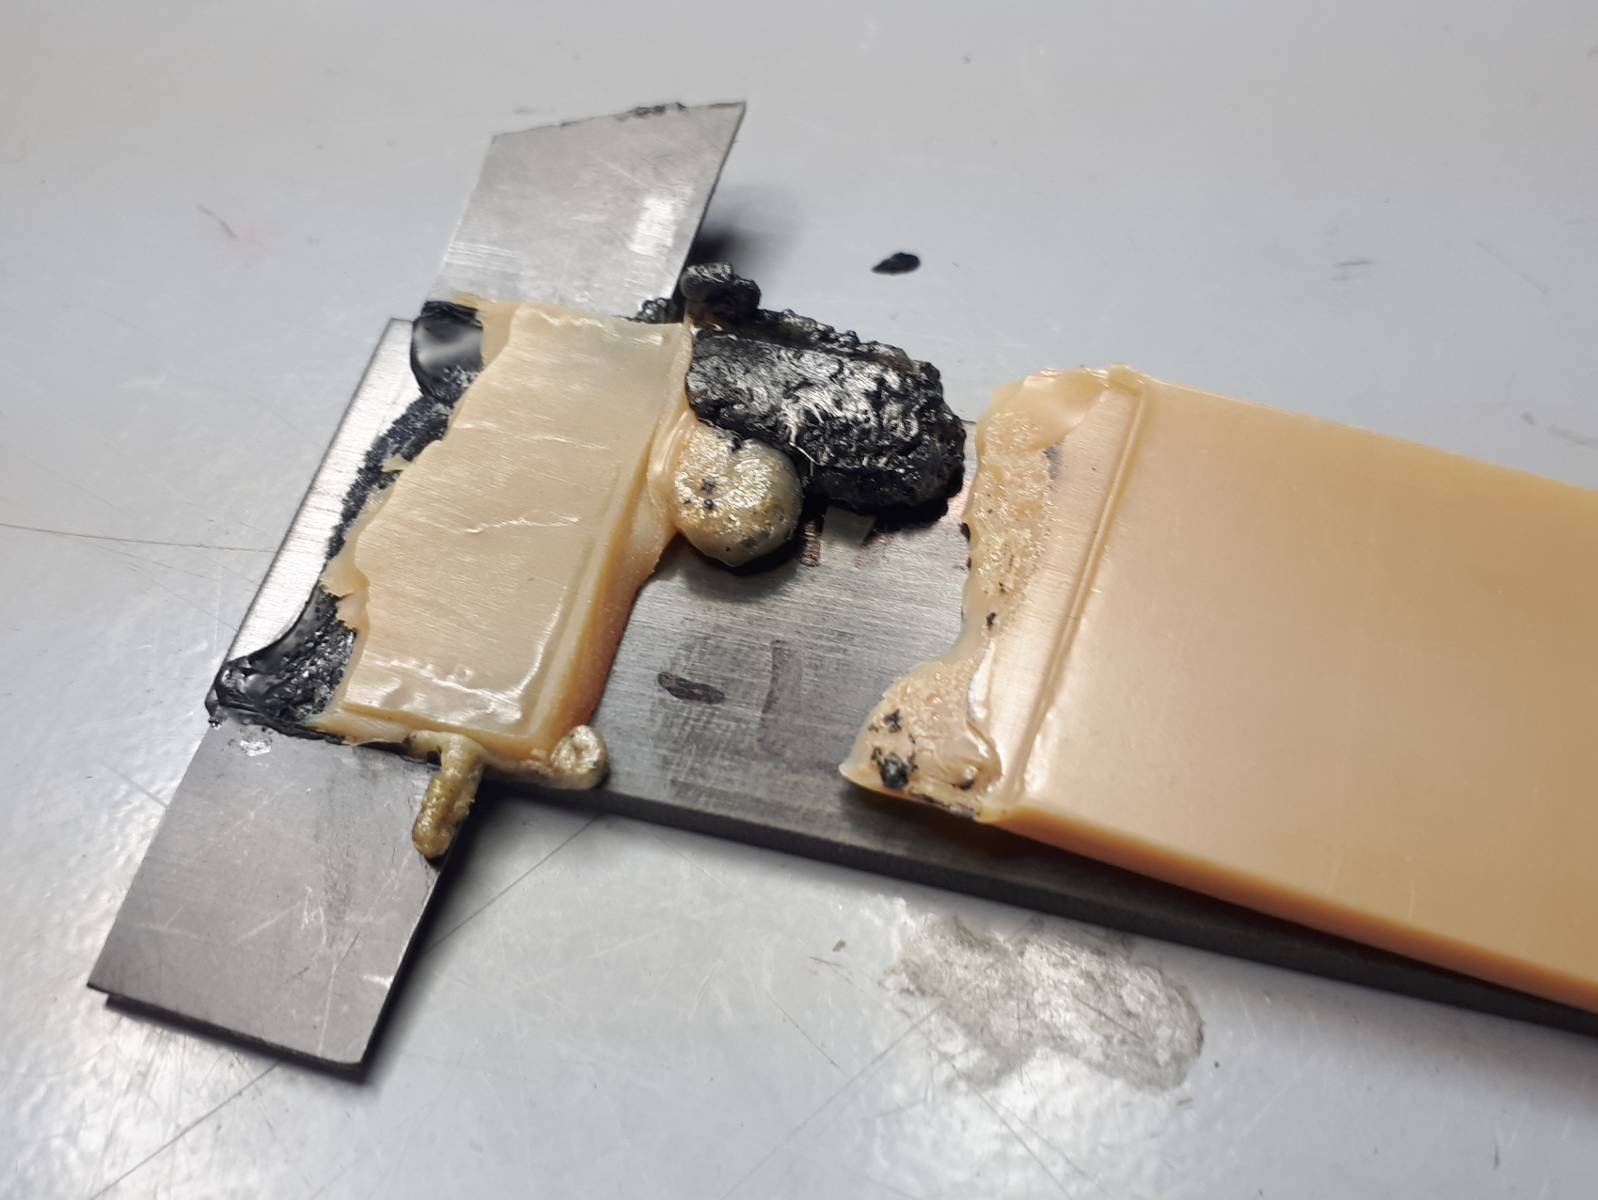
\includegraphics[height=5.5cm]{MM_300_45_crop_resize.jpg}
	} 
	\caption{Résultats des essais de soudage multimatériaux initiaux avec des paramètres de soudage a) \SI{260}{\kilo\watt\per\square\metre} pendant \SI{60}{\second}, b) \SI{220}{\kilo\watt\per\square\metre} pendant \SI{60}{\second}, c) \SI{180}{\kilo\watt\per\square\metre} pendant \SI{180}{\second} et d) \SI{300}{\kilo\watt\per\square\metre} pendant \SI{45}{\second}}
	\label{fig:MM_essais_initiaux}
\end{figure}
\FloatBarrier

La résistance des soudures obtenues a pu être évaluée par essais de simple cisaillement (Tab.~\ref{tab:LSS_multi_materiau}). 
Des temps de soudage de 35 et \SI[locale=FR]{45}{\second} ainsi que des puissances entre 220 et \SI[locale=FR]{300}{\kilo\watt\per\square\metre} ont été utilisés et permettaient d'obtenir des soudures. 
La pression sur la soudure a été réduite après les deux premières conditions de test en raison de la quantité de polymère ayant flué. 
Dans tous les cas, sauf pour la soudure réalisée avec une puissance de \SI[locale=FR]{220}{\kilo\watt\per\square\metre}, une fumée blanche a été dégagée durant le soudage. 

\begin{table}[h]
	\centering
	\caption{Essais de caractérisation mécanique de soudures multimatériaux}
	\begin{tabular}{@{}cccC{1in}c@{}}
		\toprule
		              Puissance                &       Temps        &        Pression         & Nombre d'échantillons &    LSS (Écart-type)     \\
		{[}\si{\kilo\watt\per\square\metre}{]} & {[}\si{\second}{]} & {[}\si{\mega\pascal}{]} &                       & {[}\si{\mega\pascal}{]} \\ \midrule
		                 300                   &         45         &            1            &           1           &       8,2 (S.O.)        \\
		                 300                   &         35         &            1            &           1           &       5,7 (S.O.)        \\
		                 300                   &         45         &           0,4           &           5           &        6,3 (1,0)        \\
		                 280                   &         45         &           0,4           &           2           &        4,2 (0,1)        \\
		                 260                   &         45         &           0,4           &           2           &        4,6 (0,8)        \\
		                 240                   &         45         &           0,4           &           2           &        2,6 (0,7)        \\
		                 220                   &         45         &           0,4           &           2           &        2,0 (0,2)        \\ \bottomrule
	\end{tabular}
	\label{tab:LSS_multi_materiau}
\end{table}

\begin{figure}[h]
	\centering
	\includegraphics[width=0.5\textwidth]{20190618_145038_crop_resize.jpg}
	\caption{Faciès de rupture après un essai mécanique d'une soudure multimatériau}
	\label{fig:facies_multi_materiau}
\end{figure}

Une analyse des faciès de rupture des échantillons (Fig. \ref{fig:facies_multi_materiau}) permet de voir que des conditions de soudage sous-optimales entraînent la dégradation thermique du nanocomposite. 
Sur cette figure, on peut observer une section centrale fortement dégradée ainsi que des résidus adhérés à l'élastomère. 
Une observation au microscope optique a également révélé la formation de bulles et porosités dans l'élastomère. 

La seconde série de tests employant des puissances réduites avait pour but de déterminer une puissance propice à générer une soudure, mais qui ne mènerait pas à une dégradation thermique de l'élastomère. 
L'observation des faciès obtenus lors de cette série de tests a permis de récolter un grand nombre d'informations. 
La demi-soudure entre l'élément chauffant nanocomposite et le composite a généralement été le point faible des soudures. 
Celle-ci doit en effet atteindre un état pleinement soudé après la réalisation des deux joints, mais sans atteindre la dégradation thermique. 
Il sera nécessaire d'optimiser les paramètres de la première soudure en fonction de la puissance qui sera appliquée lors de la deuxième soudure. 
Pour les joints produits avec des puissances de 260 et \SI[locale=FR]{280}{\kilo\watt\per\square\metre}, la rupture s'est produite dans le nanocomposite, du côté du composite. 
Pour ces puissances, la seconde étape de soudage a permis de compléter partiellement la première soudure. 
Pour les essais avec des puissances de 220 et \SI[locale=FR]{240}{\kilo\watt\per\square\metre}, la seconde étape de soudure n'a pas permis de compléter le premier joint alors les ruptures se sont produites entre le nanocomposite et le composite. 
Du côté de l'élastomère, à partir de \SI[locale=FR]{220}{\kilo\watt\per\square\metre}, il y a formation d'un nombre croissant de porosités en fonction de la puissance appliquée. 
À partir de \SI[locale=FR]{240}{\kilo\watt\per\square\metre} des résidus d'élastomères ont été laissés sur le nanocomposite. 
Ces résidus semblent se former lorsque la quantité de porosité à proximité de la surface de l'élastomère permet la formation d'une pellicule selon le mécanisme présenté à la figure \ref{fig:bulles_elastomere}. 
La présence de ces résidus adhérés au nanocomposite semblent indiquer la possibilité d'obtenir une soudure entre les matériaux. 

\begin{figure}[h]
	\centering
	\includegraphics[scale=1]{bulles_elastomee.pdf}
	\caption{Mécanisme de rupture de l'élastomère après une soudure multimatériau}
	\label{fig:bulles_elastomere}
\end{figure}

Afin d'éliminer tout problème pouvant avoir pour cause le nanocomposite, une soudure avec un élément chauffant en acier inoxydable a été produite. 
Pour cette soudure, une couche de PEI vierge a été laminée en surface des adhérents composites.
Un élément chauffant en grillage d'acier inoxydable a été inséré entre les adhérents de composite et d'élastomère. 
Un essai initial a été réalisé avec un thermocouple pour valider la température à l'interface. 
Avec une puissance de \SI[locale=FR]{220}{\kilo\watt\per\square\metre} la température atteint \SI[locale=FR]{320}{\celsius} après \SI[locale=FR]{45}{\second} et \SI[locale=FR]{360}{\celsius} après \SI[locale=FR]{65}{\second}. 
Les résistances mécaniques de deux échantillons, soudés avec des puissances de 200 et \SI[locale=FR]{220}{\kilo\watt\per\square\metre} pendant \SI[locale=FR]{45}{\second}, ont été évaluées respectivement à 5,6 et \SI[locale=FR]{6,9}{\mega\pascal}. 
Une observation au microscope a permis d'observer un grand nombre de porosités dans le faciès de rupture. 
Encore une fois, les porosités à l'interface cette fois combinées à la présence du grillage d'acier inoxydable ont causé une rupture cohésive de l'élastomère au niveau de l'élément chauffant. 
Outre la présence de porosité, le résidu d'élastomère semble bien adhérer au composite.  

\begin{figure}[h]
	\centering
	\subfigure[]
	{\label{fig:STM1500_facies1_soudure_SS}
		\includegraphics[height=4.25cm]{20190918_112850_crop_resize.jpg}
	} \qquad
	\subfigure[]
	{\label{fig:STM1500_facies2_soudure_SS}
		\includegraphics[height=4.25cm]{20190918_112859_crop_resize.jpg}
	}
	\caption{Faciès de rupture suite aux essais mécaniques pour l'échantillon soudé avec un élément chauffant en acier inoxydable et une puissance de \SI{220}{\kilo\watt\per\square\metre} pendant \SI{45}{\second} présentant a) le côté de l'élastomère et b) le côté du composite}
	\label{fig:STM1500_facies_soudure_SS}
\end{figure}

\FloatBarrier
\subsection{Vérification de la miscibilité du PEI-siloxane}

Un mélange de PEI avec 10\% massique de PEI-siloxane a été produit avec un mélangeur interne. 
Lors de ce mélange, le PEI a été initialement mélangé pendant 10 minutes à \SI[locale=FR]{340}{\celsius} avant d'ajouter l'élastomère et poursuivre le mélange pendant 3 minutes. 
Le mélange obtenu a été observé au microscope électronique à balayage afin d'observer la présence ou l'absence de compatibilité et de diffusion entre les phases. 
Les images obtenues (Fig. \ref{fig:SEM_mix_STM1500_PEI}) indiquent que 3 minutes n'ont pas été suffisantes pour obtenir un mélange uniforme puisqu'on dénote deux phases distinctes. 
Cependant, les structures de la section indiquée ont la même morphologie que les structures obtenues lors d'un mélange complet \cite{Hatui2015}. 
L'absence de ségrégation complète ou de fissure entre les phases supporte l'idée que 10\% de PEI-siloxane soit miscibile dans une matrice de PEI. 
Des essais supplémentaires seront cependant nécessaires pour démontrer hors de tout doute cette miscibilité puisqu'une simple observation au microscope électronique à balayage ne permet pas d'obtenir des observations à une échelle suffisante pour confirmer le phénomène. 

\begin{figure}[h]
	\centering
	\includegraphics[width=0.7\textwidth]{PEI_STM1500_09(x800).pdf}
	\caption{Observation au microscope électronique à balayage d'un mélange composé de PEI et de 10\% massique de PEI-siloxane}
	\label{fig:SEM_mix_STM1500_PEI}
\end{figure}

\FloatBarrier
\section{Conclusion}

Au vu des résultats obtenus, on peut confirmer que le PEI-siloxane présente le potentiel pour obtenir une jonction soudée. 
Cet élastomère est miscible dans le PEI jusqu'à une fraction massique supérieure à 10\%. 
Il offre également de bonnes propriétés mécaniques et une excellente stabilité thermique. 
Cependant, jusqu'à présent, il n'a pas été possible de trouver des conditions propices à l'obtention d'une bonne soudure avec une bonne diffusion des chaînes de polymères. 
Cet élastomère forme rapidement des porosités lorsqu'il est chauffé et ces dernières empêchent la formation d'une jonction solide. 
Le taux d'humidité dans l'élastomère et le PEI composant le nanocomposite n'ayant pas été pris en compte pour les soudages, il serait approprié d'au moins répéter les essais en laboratoire avec des adhérents et des éléments chauffants ayant été séchés à l'étuve. 
Une partie des porosités rencontrées dans les soudures entre adhérents composites pourrait d'ailleurs être expliquées de cette façon. 
Une autre approche qui pourrait être envisagée, à défaut d'une soudure, est de texturer l'élément chauffant pour améliorer le blocage mécanique entre les phases. 
Un autre point noté durant ces essais est que les cycles thermiques à haute température répétés pour le nanocomposite causent une dégradation de ses propriétés. 
Encore une fois, en raison de la quantité de nanotubes de carbone dans le nanocomposite, la diffusion des chaînes de polymères est ralentie et nécessite des températures élevées qui sont propices à la dégradation des polymères. 
Cet effet était visible dans la fenêtre d'opération pour le soudage d'adhérents composites et il a de nouveau un impact pour la production de soudures multimatériaux. 
Les travaux afin d'obtenir un soudage multimatériaux n'ont pas permis, pour l'instant, d'aboutir à une solution rencontrant les requis techniques d'ArianeGroup.              % Troisième thème (Doctorat) ou effacez ce fichier si vous êtes à la Maîtrise.
\selectlanguage{french}
\Chapter{DISCUSSION GÉNÉRALE}\label{sec:Discussion}

\section{Autres travaux}

Les articles présentés dans le cadre de cette thèse ne constituent qu'une portion de l'ensemble des travaux réalisés. 
Ce chapitre présente une partie de ces travaux supplémentaires. 

\subsection{Conception du montage de soudage par résistance}

Afin de pouvoir réaliser des essais de soudage, il a été nécessaire de concevoir et de fabriquer un système de soudage par résistance. 
La conception du montage a nécessité de définir la géométrie du montage, le choix de la source, le système d'acquisition de données et l'interface de contrôle. 
Le montage de soudage a été conçu itérativement.
Au total, 3 versions ont été développées avant d'obtenir la configuration finale. 
Le système produit vise à être polyvalent et pourra servir à de nombreux projets de recherche. 

À la suite des essais de soudage initiaux, la flexibilité du système de soudage a d'ailleurs été requise pour régler des problèmes de répétabilité. 
En raison de variations dans les dimensions des éléments chauffants et d'un mode de contrôle en voltage constant, la puissance dissipée dans les joints variait énormément d'un essai à l'autre. 
Développer le mode de contrôle en puissance constante a permis de stabiliser la quantité d'énergie dissipée dans le joint et d'obtenir des résultats répétables. 
Désormais, même lors d'essais de soudage avec des éléments chauffants en acier inoxydable, la variation de résistance causée par l'augmentation de température ne vient plus affecter la quantité d'énergie dissipée lors de l'utilisation du mode de contrôle en puissance constante. 

Le montage de soudage est contrôlé à l'aide d'une interface graphique permettant de configurer tous les paramètres du procédé et d'enregistrer de façon synchrone les conditions d'opération (températures, forces, voltage, courant, etc. ). 

\FloatBarrier
\subsection{Résistance de contact des électrodes}

Dès le début des essais de soudage, des modèles simplifiés étaient développés en parallèle. 
En raison de divergences entre les mesures de température et les valeurs prévues lors des premiers essais, l'effet de la pression des électrodes contre le nanocomposite sur la résistance de contact a été évalué (Fig. \ref{fig:resistance_contact}). 
Une amélioration de la méthode de mesure de la résistance de contact, en isolant sur le plan électrique la section mesurée, a d'ailleurs été un élément clé pour l'élaboration du modèle présenté au chapitre \ref{sec:Theme2}. 

\begin{figure}[h]
	\centering
	\includegraphics[width=0.75\textwidth]{contact_resistance.pdf}
	\caption{Effet de la pression sur la résistance de contact entre les électrodes de cuivre et le nanocomposite}
	\label{fig:resistance_contact}
\end{figure}

\FloatBarrier
\subsection{Analyse des porosités dans les joints}

Pour évaluer l'effet de la pression durant le soudage et pour assurer des joints de qualité satisfaisante, des micrographies ont été prises afin d'identifier la présence de porosités (Fig. \ref{fig:micro_analyse_porosite}). 
Les échantillons pour ces observations sont produits à partir de tranches présentant le centre et le bord de la soudure. 

\begin{figure}[h!]
	\centering
	\subfigure[]
	{\label{fig:micro_joint_sans_porosite} 								\includegraphics[width=0.45\textwidth]{0_6MPa_Milieu_01_bw.jpg}
	} \qquad
	\subfigure[]
	{\label{fig:micro_joint_avec_porosite}
		\includegraphics[width=0.45\textwidth]{1_4MPa_Milieu_02_bw_anotate.jpg}
	}
	\caption{Micrographies d'échantillons soudés ayant servi à l'analyse des porosités dans les joints présentant a) l'absence de porosités et b) la présence de porosités}
	\label{fig:micro_analyse_porosite}
\end{figure}

\FloatBarrier
\section{Synthèse des travaux}

%Les objectifs poursuivis dans le cadre de cette thèse se déclinaient comme suit : 
%
%\begin{enumerate}
%	\item Concevoir un élément chauffant nanocomposite conducteur en tenant compte des propriétés électriques et thermiques nécessaires au procédé de soudage par résistance. 
%	\item Développer un procédé de soudage par résistance avec un élément chauffant nanocomposite entre deux adhérents en composite à matrice thermoplastique. 
%	\item Établir une fenêtre d'opération pour le soudage par résistance avec un élément chauffant nanocomposite entre deux adhérents en composite à matrice thermoplastique. 
%	\item Développer un procédé de soudage par résistance avec un élément chauffant nanocomposite entre un adhérent en composite à matrice thermoplastique et un adhérent en élastomère thermoplastique. 
%\end{enumerate}

En premier lieu, un nanocomposite conducteur a été conçu et caractérisé. 
Pour ce faire, plusieurs compositions de nanocomposites ont été produites et évaluées. 
La composition démontrant les meilleures caractéristiques a été produite en plus grande quantité et utilisée pour démontrer la possibilité de l'utiliser comme élément chauffant. 
La preuve de concept du procédé de soudage utilisant ce nanocomposite a permis de valider le concept d'un élément chauffant nanocomposite. 

En second lieu, un modèle par éléments finis a été développé afin d'établir les limites de la fenêtre d'opération du procédé de soudage. 
Des essais de soudage supplémentaires en laboratoire sont venus confirmer la fenêtre identifiée. 
Grâce à un meilleur contrôle du procédé, il a été possible d'améliorer les performances mécaniques des joints. 

Finalement, la production de jonctions soudées flexibles à l'aide du procédé de soudage résistif a été explorée et quelques avancées ont été obtenues. 
Cette exploration a mené à la sélection du PEI-siloxane commercial ULTEM STM1500 qui est compatible avec le PEI. 
Cependant, les travaux de cette thèse n'ont pas permis de trouver des paramètres opérationnels permettant d'obtenir un soudage multimatériaux rencontrant les requis techniques d'ArianeGroup. 
Certaines pistes supplémentaires ont été identifiées telles que le taux d'humidité dans le nanocomposite et l'élastomère ainsi que la possibilité de texturer le nanocomposite. 

Les objectifs 1 à 3, présentés à la section \ref{sec:objectifs}, ont été couverts et atteints par les articles présentés aux chapitres \ref{sec:Theme1} et \ref{sec:Theme2}. 
Le premier article \cite{Brassard2019a} a été publié en février 2019 dans la revue \textit{Composites Part B: Engineering} après révision par les pairs. 
Cet article a déjà été reconnu et cité par d'autres chercheurs travaillant au développement de nouveaux éléments chauffants pour le soudage des composites à matrice thermoplastique \cite{Russello2019,Su2020,Bhudolia2020,Bhudolia2020a}. 
Le second article a été soumis au journal \textit{Composites Part B: Engineering} en octobre 2019 et est en attente de révision par les pairs. 
En ce qui concerne l'objectif 4, ce dernier fait l'objet du chapitre \ref{sec:Theme3}. 
\selectlanguage{french}
\Chapter{CONCLUSION ET RECOMMANDATIONS}\label{sec:Contributions}

\section{Contributions originales}

La recherche de nouveaux éléments chauffants a permis au soudage résistif de passer initialement d'éléments chauffants en fibres de carbone vers des éléments chauffants en acier inoxydable. 
Il est donc naturel dans ce domaine de poursuivre les recherches pour développer de nouvelles solutions. 
Dans sa forme actuelle, l'élément chauffant présenté dans le cadre de cette thèse n'est pas un substitut direct pour un grillage en acier inoxydable, mais plutôt un complément. 
Il présente des limitations tout en bénéficiant d'avantages distincts.
Au niveau des propriétés mécaniques, avec un nanocomposite contenant 10\% massique de nanotubes de carbone, les essais en laboratoire ont permis d'obtenir une résistance en cisaillement maximale moyenne de \SI{24.9}{\mega\pascal}. 
De plus, les résultats des essais de cisaillement, pour l'ensemble des points se situant dans la fenêtre d'opération, se retrouvent tous à l'intérieur de la plage d'intervalle de confiance à 95\%. 
Les variations visibles des moyennes présentées (Fig.~\ref{fig:2_Fig7}) proviennent donc simplement de fluctuations normales et aucun ensemble de paramètres en particulier ne se détache du lot. 
Ces résultats restent également inférieurs aux résistances pouvant être obtenues avec un élément chauffant en acier inoxydable qui peuvent atteindre jusqu'à \SI{50}{\mega\pascal}. 
Toutefois, cette recherche ouvre la porte vers une nouvelle classe d'éléments chauffants qui s'intègrent totalement dans la pièce obtenue. 
Ces travaux pourront servir de base à des recherches visant à raffiner cette première itération. 
De plus, comme pour les matériaux composites, les éléments chauffants nanocomposites peuvent être adaptés à l'application spécifique où ils seront employés. 
Ils pourraient, par exemple, être intégrés à des composants afin de servir d'éléments chauffants pour le dégivrage. 
Également, leur conductivité électrique pourrait être utilisée dans les systèmes de protection contre la foudre des aéronefs en composite, et ce, en assurant une continuité électrique entre les composants assemblés. 
Les échantillons en nanocomposite présentent encore un énorme potentiel pour la recherche et son application. 

Dans le cadre de la revue de la littérature concernant le soudage par résistance, le contrôle de la source avec une puissance constante n'a jamais été présenté avant cette thèse.  
Ce mode d'opération permet un meilleur contrôle de la puissance dissipée dans le joint et permet d'éliminer l'effet de la variation de résistance de l'élément chauffant, que l'on rencontre même avec les éléments chauffants en acier inoxydable. 
Même si le développement de ce mode d'opération devenait nécessaire pour les éléments chauffants nanocomposites de ce projet, il a néanmoins permis d'améliorer le contrôle du procédé de soudage lors de la production de joints avec un élément chauffant en acier inoxydable, selon les observations d'un collègue travaillant avec ce type d'élément chauffant. 

Finalement, même si le soudage multimatériaux existe dans le cas de liaisons entre des composites thermoplastiques et des composites thermodurcissables \cite{FernandezVillegas2015,Lionetto2018a} ou encore pour des liaisons entre des composites thermoplastiques et des métaux \cite{Weidmann2018,Kruger2004,Balle2009,Goushegir2016}, aucun cas documenté n'existe pour le soudage d'une jonction flexible. 
La preuve de la nécessité de ce type de jonction provient de la problématique initiale de cette thèse.
Notre partenaire, ArianeGroup, recherche un type de jonction qui n'existe tout simplement pas encore sur le marché et ces travaux de recherche ont eu pour but de répondre à ce besoin. 
Les adhésifs peuvent remplir une partie de leurs requis à court terme, mais les problèmes de sensibilité aux contaminants et le manque de robustesse de ces jonctions force le développement de nouvelles solutions. 
Bien qu'aucune soudure rencontrant les requis du cahier des charges n'ait été produite pour le moment, poser les bases théoriques constitue déjà une contribution originale dans l'optique de développer éventuellement une solution appliquée à leurs besoins. 
De plus, les travaux présentés ont permis de sélectionner le copolymère multiblocs PEI-siloxane comme candidat potentiel pour obtenir des soudures. 

\section{Limites et recommandations}

Les solutions développées dans le cadre de cette thèse ne sont pas sans failles. 
Bien identifier leurs limites permet de cerner des pistes d'amélioration et de formuler des projets de recherche subséquents. 

Tout d'abord, au vu d'éléments complémentaires trouvés tout au long du projet, il a été établi que l'utilisation de la méthode FTIR présentée en annexe du premier article (voir Annexe \ref{sec:Annexe_B}) n'était pas la bonne façon de déterminer la présence ou l'absence de dégradation. 
Le spectre présenté (Fig.~\ref{fig:FTIR_spectra}) est de piètre qualité et ne fournit aucune information utile quant à l'état de dégradation du nanocomposite. 
La figure est cependant conservée dans cette thèse, puisqu'elle fait partie des documents complémentaires publiés avec l'article. 
Afin de valider l'absence de dégradation du PEI qui entrainerait une réduction de ses propriétés mécaniques, il serait approprié de réaliser des mesures de la masse moléculaire du PEI après le procédé de soudage. 

Également, lors des essais de soudage, les conditions hygrothermiques des matériaux n'ont pas été considérées malgré l'importance qu'elles peuvent avoir. 
Les porosités observées aux interfaces ainsi que dans l'élastomère peuvent provenir de l'absence de contrôle de ce paramètre clé. 
Ce facteur aurait dû être pris en compte et devra certainement être considéré lors des développements futurs. 

Un élément ayant été intégré tardivement au projet est l'enrichissement des surfaces à souder avec des films de PEI. 
L'absence des films de PEI a fait en sorte que les températures nécessaires au soudage n'étaient plus dans la plage suggérée pour un procédé de soudage avec un film de polymère amorphe, en plus de nécessiter la fusion complète du PEEK. 
Les prochains essais de soudages devraient donc intégrer des films de PEI en surface afin de réduire les températures nécessaires.  

Dans un même ordre d'idée, l'incapacité d'obtenir une mesure directe de la température est une limite rencontrée durant ce projet. 
Il aurait été très utile de pouvoir mesurer le champ de température à l'interface entre le nanocomposite et les adhérents afin de mieux comprendre les processus de dégradation et d'interdiffusion. 
Une suite de ce projet devrait tenter de développer une méthode permettant cette mesure. 

Une grande limitation du soudage à l'aide d'un élément chauffant nanocomposite, dans sa forme actuelle, réside dans son incapacité à produire des soudures avec des laminés autres qu'unidirectionnels. 
La plus faible conductivité électrique du nanocomposite par rapport à celle des éléments chauffants en acier inoxydable rend les éléments chauffants plus susceptibles aux fuites de courant au travers du laminé quand des fibres de carbone sont alignées dans le même sens que le courant. 
Lors du soudage, les voltages appliqués sont approximativement douze fois plus élevés que lorsqu'un élément chauffant en acier inoxydable est employé. 
En optimisant la nature du nanocomposite ou en augmentant le nombre de nanotubes de carbone, il serait possible d'obtenir des conductivités plus élevées qui réduiraient ce phénomène. 
Afin de résoudre ce problème, quelques pistes de solutions peuvent être envisagées. 

\begin{itemize}
	\item Développer un traitement de fonctionnalisation des nanotubes qui permettra de réduire la résistance de contact et ainsi obtenir une plus grande conductivité.  
	\item Considérer l'emploi de plusieurs types de nanoparticules pour tirer profit de l'effet de synergie et obtenir des conductivités électriques plus élevées. 
	\item Ajouter des couches de PEI vierge de chaque côté du nanocomposite, moulées avec l'élément chauffant ou en tant que films intercalés, afin d'agir comme isolant et d'aider à réduire les risques de fuites de courant. 
\end{itemize}

Cependant, un équilibre doit être conservé en ce qui concerne la composition du nanocomposite. 
Une grande quantité de nanotubes dans le nanocomposite limite la mobilité des chaines de polymères. 
Ceci entraine des difficultés lors de la mise en forme du nanocomposite, mais plus particulièrement lors du soudage.
En raison de la faible mobilité des chaines, il est nécessaire de chauffer le joint à des températures plus élevées. 
Ce niveau de chauffe cause des problèmes de dégradation thermique du nanocomposite. 
La faible mobilité des chaines de polymères en raison de la quantité de nanotubes peut également expliquer une partie des problèmes rencontrés lors des essais de soudage multimatériaux. 
Ce facteur pousse vers des nanocomposites avec une fraction massique plus faible de nanotubes de carbone. 
En ce sens: 

\begin{itemize}
	\item Des traitements de fonctionnalisation des nanotubes pourraient permettre non seulement d'augmenter la conductivité du composite, mais également d'utiliser un plus petit nombre de nanotubes afin de limiter leur effet sur la mobilité des chaines de polymères. 
	\item L'emploi de plusieurs types de nanoparticules pour tirer profit de l'effet de synergie afin de réduire les quantités totales de nanoparticules nécessaires pourrait être considéré. 
	\item Il faudrait déterminer plus précisément l'effet des charges sur le temps de reptation des chaines de polymères et l'impact que cela entraine sur les conditions de soudure. 
	Cet effet devrait être pris en compte lors de l'optimisation de la composition de l'élément chauffant. 
	\item Afin de limiter les contraintes thermiques imposées au nanocomposite, il faudrait explorer la possibilité de surmouler les éléments chauffants ou de les intégrer durant la fabrication des composants. 
	Il pourrait être nécessaire d'insérer des couches isolantes entre le composite et l'élément chauffant. 
	En plus d'agir comme isolant, si ces couches étaient des films de PEI vierge, elles pourraient fournir, à l'interface du joint soudé, un milieu exempt de nanocharges avec une plus grande mobilité des chaines de polymères que dans le nanocomposite lui-même. 
	\item Après avoir modifié la composition de l'élément chauffant, il faudrait évaluer l'effet  des modifications sur la fenêtre de procédé. 
	Augmenter la mobilité des chaines pourrait permettre d'élargir la fenêtre d'opération et éviter d'opérer à proximité des conditions menant à la dégradation du nanocomposite. 
\end{itemize}

Une autre limite en ce qui a trait au soudage réside dans la faible résilience mécanique du nanocomposite. 
En raison de la quantité de nanotubes, le nanocomposite présente un comportement purement élastique sans plateau plastique lors d'essais de traction. 
Des ruptures fragiles ont pu être observées non seulement lors des essais mécaniques avec le nanocomposite, mais également lors de l'analyse des faciès de rupture des joints soudés. 
Une augmentation de la résilience du nanocomposite pourrait être obtenue en réduisant le chargement en nanotubes de carbone. 
En ce sens: 

\begin{itemize}
	\item Il faudrait quantifier l'effet de l'ajout de nanoparticules sur la ductilité des nanocomposites et trouver une composition permettant un compromis entre les requis de conductivité électrique et la résilience. 
\end{itemize}

Un PEI avec une faible masse moléculaire a été sélectionné pour la fabrication du nanocomposite. 
Ce PEI avait l'avantage de réduire le temps nécessaire à la reptation des chaines, mais en offrant des propriétés mécaniques réduites. 
Afin d'augmenter la résistance mécanique du nanocomposite, il serait intéressant d'évaluer la possibilité d'utiliser du PEI à chaines longues ou, encore, un mélange de PEI avec diverses longueurs de chaines. 

Les travaux actuels n'ont pas permis d'arriver à des conclusions quant au niveau d'interdiffusion des chaines de polymères ni à la compatibilité entre l'élastomère et la matrice du nanocomposite. 
Un prochain projet devra aborder ces enjeux. 
Tout d'abord, une analyse formelle de la compatibilité à l'aide de la théorie de Flory-Huggins permettra de confirmer la possibilité d'obtenir un mélange des polymères. 
Après cela, un travail approfondi devra mesurer l'évolution de l'interdiffusion dans les interfaces soudées en caractérisant la diffusion de la matrice du nanocomposite et des adhérents, et de l'élastomère. 
Ces travaux pourront servir de fondation afin d'améliorer le procédé de soudage. 

Finalement, la conception initiale du nanocomposite avait comme seul critère la conductivité électrique. 
Cette cible peut être atteinte de plusieurs façons. 
La solution actuelle, atteignant la cible de conductivité électrique, présente fort probablement un haut niveau d'agglomération des nanotubes de carbone. 
Ces agglomérats empêchent de tirer pleinement profit des propriétés des nanotubes de carbone. 
Une prochaine boucle d'optimisation du nanocomposite devrait prendre en compte l'état de dispersion des charges conductrices. 

Comme on peut le constater, la nature du nanocomposite est un sujet dont devraient traiter les prochaines recherches à propos du soudage avec un élément chauffant nanocomposite. 
La composition actuelle a permis de démontrer le procédé, mais considérer uniquement la conductivité électrique lors du choix de composition n'est pas suffisant pour obtenir un bon élément chauffant.
Effectuer des boucles itératives quant à la nature et à la composition du nanocomposite permettrait d'optimiser les matériaux pour le procédé de soudage par résistance. 

En ce qui concerne le soudage multimatériaux, les jonctions obtenues n'ont pas rencontré les requis du cahier des charges. 
Il y a cependant quelques pistes de recherches qui nécessiteraient d'être poussées plus loin. 

\begin{itemize}
	\item Les conditions de soudage évaluées utilisaient des puissances relativement élevées et des temps de soudages très courts. 
	Il serait approprié d'explorer des temps de soudage plus long avec des puissances plus faibles afin de réduire les contraintes thermiques sur l'élastomère. 
	\item Il faudrait sécher les adhérents et les éléments chauffants pour éliminer l'effet de l'humidité absorbée. 
	Il est déjà documenté que la présence d'humidité dissoute dans un composite peut mener à l'apparition de porosités dans un joint soudé par résistance \cite{Shi2014}. 
	\item Finalement, une soudure n'est pas l'unique façon d'obtenir une jonction entre des composants. 
	L'utilisation d'une surface texturée augmentant la rugosité peut permettre d'obtenir un blocage mécanique entre les phases pour certains types de chargement. 
	Ces joints n'atteindront pas les performances de jonctions soudées, mais ils pourraient rencontrer les requis pour certaines applications. 
\end{itemize}

Le développement initial d'un élément chauffant nanocomposite s'inscrit dans le continuum de la recherche pour le soudage résistif des matériaux composites. 
Ce projet n'est pas une finalité, mais un tremplin vers le développement de nouvelles solutions. 		% Description des contributions du projet de recherche, analyse critique des résultats et conclusion
% \selectlanguage{french}
\Chapter{CONTRIBUTIONS ET CONCLUSION}\label{sec:Contributions}

\section{Synthèse des travaux}

Les objectifs poursuivis dans le cadre de cette thèse se déclinaient comme suit : 

\begin{enumerate}
	\item Développer un nanocomposite conducteur pouvant servir d'élément chauffant dans un procédé de soudage par résistance. 
	\item Produire une soudure par résistance entre des adhérents en composites thermoplastiques. 
	\item Établir une méthode de soudage par résistance pour la production d'une jonction flexible intégrant un élastomère thermoplastique entre des adhérents en composites thermoplastiques. 
\end{enumerate}

Les travaux de cette thèse atteignent en partie ces objectifs. 
En premier lieu, un nanocomposite conducteur a été développé et caractérisé. 
Pour ce faire, plusieurs compositions de nanocomposite ont été produites et évaluées. 
La composition démontrant les meilleures caractéristiques a été produite en plus grande quantité et utilisée pour démontrer la possibilité de l'utiliser comme élément chauffant. 
En second lieu, le processus de soudage a été modélisé à l'aide d'un modèle par éléments finis afin d'établir une fenêtre de procédé. 
Des essais de soudage supplémentaires sont venus renforcer notre contrôle du procédé et ont permis de valider la fenêtre proposée. 
Finalement, la production de jonctions soudées flexibles à l'aide du procédé de soudage résistif a été explorée. 
Cette exploration a mené à la sélection du ULTEM STM1500 qui est compatible avec le PEI. 
Ces travaux n'ont cependant pas permis de déterminer des paramètres permettant d'obtenir un soudage multi matériau. 

Les objectifs 1 et 2 ont été couverts et atteints par les articles présentés aux chapitres \ref{sec:Theme1} et \ref{sec:Theme2}. 
Le premier article \cite{Brassard2019a} a été publié en février 2019 dans la revue \textit{Composites Part B: Engineering} après révision par les pairs. 
Cet article a déjà été reconnu et cité par d'autres chercheurs travaillant au développement de nouveaux éléments chauffants pour le soudage des composites à matrice thermoplastique \cite{Russello2019}. 
Le second article a été soumis au journal \textit{Composites Part B: Engineering} en octobre 2019 et est en attente de révision par les pairs après avoir été accepté par l'éditeur. 
En ce qui concerne l'objectif 3, ce dernier fait l'objet du chapitre \ref{sec:Theme3}. 
Certains travaux toujours en cours pourraient venir permettre de le compléter afin de préparer un troisième article.

\section{Contributions originales}

La recherche de nouveaux éléments chauffants a permis au soudage résistif de passer initialement d'éléments chauffants en fibre de carbone vers des éléments chauffants en acier inoxydable. 
Il est naturel dans ce domaine de poursuivre les recherches de nouvelles solutions \cite{Russello2019}. 
Dans sa forme actuelle, l'élément chauffant présenté dans le cadre de cette thèse n'est pas un substitut direct pour un grillage en acier inoxydable. 
Il présente des limitations.
Cependant il ouvre la porte vers une nouvelle classe d'éléments chauffants qui s'intègrent totalement dans la pièce obtenue. 
Ces travaux pourront servir de base à des recherches visant à raffiner cette première itération. 
De plus, comme pour les matériaux composites, les éléments chauffants nanocomposites peuvent être adaptés à l'application spécifique où ils seront employés. 
Un potentiel encore inexploré s'offre à eux. 

Dans un second temps, même si le soudage multi matériaux existe dans le cas de composites thermoplastiques et de composites thermodurcissables \cite{FernandezVillegas2015,Lionetto2018a} ou encore de composites thermoplastiques et de métaux \cite{Weidmann2018,Kruger2004,Balle2009,Goushegir2016}, aucun cas documenté n'existe pour le soudage d'une jonction flexible. 
Ce type de soudure n'a tout simplement jamais été réalisé. 
La preuve de la nécessité de ce type de jonction provient de la justification initiale de ce doctorat.
Notre partenaire, ArianeGroup, recherche un type de jonction qui n'existe tout simplement pas encore sur le marché et ces travaux de recherche ont eu pour but de répondre à ce besoin. 
Bien qu'aucune soudure rencontrant les requis du cahier des charges n'ait été produite, poser les bases afin de répondre éventuellement à ce besoin constitue déjà, en elle seule, une contribution originale. 

%%
%%  LIMITATIONS
%%
\section{Limitations et pistes d'amélioration}

Les solutions développées dans le cadre de ce doctorat ne sont pas sans failles. 
Bien identifier leurs limites permet de cerner des pistes d'amélioration et de formuler des projets de recherche subséquents. 

Une grande limitation du soudage à l'aide d'un élément chauffant nanocomposite, dans sa forme actuelle, réside dans son incapacité à produire des soudures avec des laminés autres qu'unidirectionnels. 
La plus faible conductivité électrique du nanocomposite par rapport aux éléments chauffants en acier inoxydable les rend plus susceptibles aux fuites de courant au travers du laminé quand des fibres de carbone sont alignées dans le même sens que le courant. 
Lors du soudage, les voltages appliqués sont approximativement douze fois plus élevés lorsqu'un élément chauffant nanocomposite est employé. 
En optimisant la nature du nanocomposite ou en augmentant le nombre de nanotubes de carbone, il serait possible d'obtenir des conductivités plus élevées qui réduiraient ce phénomène. 

Cependant, une balance doit être conservée en ce qui concerne la composition du nanocomposite, une grande quantité de nanotubes dans le nanocomposite limite la mobilité des chaînes de polymère. 
Ceci entraîne des difficultés lors de la mise en forme du nanocomposite, mais plus particulièrement lors du soudage.
En raison de la faible mobilité des chaînes, il est nécessaire de chauffer le joint à des températures plus élevées. 
Ce niveau de chauffe cause des problèmes de dégradation thermique du nanocomposite. 
Même pour les soudures réussies, on peut remarquer un début de dégradation thermique lors de l'observation des faciès de rupture. 
La faible mobilité des chaînes de polymère en raison de la quantité de nanotubes peut également expliquer une partie des problèmes rencontrée lors des essais de soudage multi matériaux. 
Ce facteur pousse vers des nanocomposites avec une fraction massique plus faible de nanotubes de carbone. 

Une autre limite en ce qui a trait au soudage réside dans la faible résilience mécanique du nanocomposite. 
En raison de la quantité de nanotubes, le nanocomposite présente un comportement purement élastique sans plateau plastique lors d'essais de traction. 
Des ruptures fragiles ont pu être observées non seulement lors des essais mécaniques avec le nanocomposite, mais également lors de l'analyse des faciès de rupture des joints soudés. 
Une augmentation de la résilience du nanocomposite pourrait également être obtenue en réduisant le chargement en nanotubes de carbone. 

Comme on peut le voir, la nature du nanocomposite sera le sujet que devraient traiter les prochaines recherches à propos du soudage avec un élément chauffant nanocomposite. 
La composition actuelle a permis de démontrer le procédé, mais considérer uniquement la conductivité électrique lors du choix de composition n'est pas suffisant pour obtenir un bon élément chauffant.

\section{Recherches futures}

Afin de répondre aux défis mentionnés dans la précédente section, plusieurs pistes de recherche sont possibles.  
La conductivité électrique, la résilience et la mobilité des chaînes de polymères devront être considérées pour la prochaine génération d'élément chauffant. 
Les améliorations requises nécessiteront des travaux sur plusieurs plans : 

\begin{itemize}
	\item Développer un traitement de fonctionnalisation des nanotubes qui permettra de réduire la résistance de contact et ainsi obtenir une plus grande conductivité avec un plus petit nombre de nanotubes. 
	\item Quantifier l'effet de l'ajout de nanoparticules sur la ductilité des nanocomposites et trouver une composition permettant d'équilibrer les requis de conductivité électrique avec les requis de résilience. 
	\item Déterminer plus précisément l'effet des charges sur le temps de reptation des chaînes de polymères et l'impact que cela entraîne sur les conditions de soudure. Cet effet devra également être pris en compte pour établir la composition de l'élément chauffant. 
	\item Afin de limiter les contraintes thermiques imposées au nanocomposite, il faudrait explorer la possibilité de surmouler les éléments chauffants ou de les intégrer durant la fabrication des composants. Il est possible qu'il soit nécessaire d'insérer des couches isolantes entre le composite et l'élément chauffant. 
	\item Après avoir modifié la composition de l'élément chauffant, il faudra évaluer l'effet  des modifications sur la fenêtre de procédé. Augmenter la mobilité des chaînes pourrait permettre d'élargir la fenêtre d'opération et éviter d'opérer à proximité des conditions menant à la dégradation du nanocomposite. 
	\item Dans le contexte du soudage multi matériaux, les soudages obtenus ont été produits avec des puissances relativement élevées et des temps de soudages très courts. Peut-être serait-il également approprié d'explorer des temps de soudage plus long avec des puissances plus faibles. 
	\item Bien entendu, un nanocomposite conducteur n'est peut-être pas la solution finale dans cette exploration pour découvrir de nouveaux éléments chauffants. La découverte de nouvelles alternatives doit être encouragée. 
	\item Finalement, une soudure n'est pas l'unique façon d'obtenir une jonction entre des composants. L'utilisation d'une surface texturée augmentant la rugosité peut permettre d'obtenir un blocage mécanique entre les phases pour certains types de chargement. Ces joints n'atteindront pas les performances de jonctions soudées, mais ils peuvent rencontrer les requis pour certaines applications. 
\end{itemize}

Le développement initial d'un élément chauffant nanocomposite s'inscrit dans le continuum de la recherche pour le soudage résistif des matériaux composites. 
Ce projet n'est pas une finalité, mais un tremplin vers le développement de nouvelles solutions.          % Conclusion.
%\backmatter
\ifthenelse{\equal{\Langue}{english}}{
%	\renewcommand\bibname{REFERENCES}
%	\bibliography{Bibliographie}
%	\bibliographystyle{IEEEtran}			% Bibliography style. 
}{
	\renewcommand\bibname{RÉFÉRENCES}
	\bibliography{Bibliographie}
	%\bibliographystyle{IEEEtran-francais}    % Style de la bibliographie. 
	\bibliographystyle{unsrtnat}
	%\bibliographystyle{plain}
}
%
\ifthenelse{\equal{\AnnexesPresentes}{O}}{
	\appendix%
	\newcommand{\Annexe}[1]{\annexe{#1}\setcounter{figure}{0}\setcounter{table}{0}\setcounter{footnote}{0}}%
	%%
%%  Annexes
%%
%%  Note: Ne pas modifier la ligne ci-dessous. / Do not modify the following line.
\ifthenelse{\equal{\Langue}{english}}{
	\addcontentsline{toc}{compteur}{APPENDICES}
}{
	\addcontentsline{toc}{compteur}{ANNEXES}
}
%%
%%
%%  Toutes les annexes doivent être inclues dans ce document
%%  les unes à la suite des autres.
%%  All annexes must be included in this document one after the other.
\Annexe{Matériaux élastomères alternatifs}
\label{sec:Annexe_A}

En plus des essais présentés concernant le PEI-siloxane, des élastomères SIS et SEBS ont été initialement évalués pour ce projet. 
Ces matériaux ont été sélectionnés par Adrien Métafiot durant une partie de son doctorat à l'université McGill. 

\section{Matériaux}

Les deux élastomères initialement évalués étaient : 
\begin{inparaenum}[]
	\item un copolymère triblocs polystyrène-b-polyisoprène-b-polystyrène (SIS) possédant une fraction molaire de styrène de 22\% (Sigma-Aldrich \#432415) et 
	\item un copolymère triblocs linéaire polystyrène-b-poly(éthylène-butylène)-b-polystyrène (SEBS) produit par Kraton\textregistered \ sous le numéro de désignation A1536 H. 
\end{inparaenum}
Les copolymères triblocs possèdent une structure générale où un segment est inséré au milieu de deux segments possédant une composition différente au segment central (Fig.~\ref{fig:polymere_tri_bloc}). 

\section{Caractérisation de la stabilité thermique des élastomères}

Des analyses thermogravimétriques (TGA) de l'élastomère ont été réalisées par Adrien Métafiot avec un appareil TA Instruments Q50. 
Deux types d'analyses ont été réalisés. 
Dans un premier temps, comme présenté dans la norme ASTM E2550 - 17, les échantillons ont été soumis à une rampe de \SI[locale=FR]{10}{\celsius\per\minute} jusqu'à une température de \SI[locale=FR]{575}{\celsius} sous une atmosphère régulière et sous une atmosphère d'azote. 
Par la suite, certains échantillons ont également été testés en condition isotherme autant avec une atmosphère d'air qu'avec une atmosphère d'azote pour évaluer la stabilité thermique dans le temps de l'élastomère. 
Ce second type d'analyse ne fait pas l'objet d'une norme standardisée de l'ASTM. 

\section{Stabilité thermique des élastomères}

Les mesures de thermogravimétrie réalisées par Adrien Métafiot à McGill ont permis d'observer le comportement thermique des élastomères SIS et SEBS. 
Dans un premier temps, un élastomère copolymère SIS commercial a été évalué. 
Les essais de caractérisation thermique (Fig.~\ref{fig:TGA_SIS}) ont rapidement indiqué que ce matériau ne rencontrerait pas les requis techniques. 
Même après un traitement d'hydrogénation, ses performances mécaniques restaient insuffisantes. 
À son état vierge, le SIS commercial s'est dégradé rapidement au-dessus d'une température de \SI[locale=FR]{320}{\celsius} (Fig.~\ref{fig:TGA_SIS_vierge}) tandis qu'après le traitement d'hydrogénation, l'élastomère a conservé 99,5\% de sa masse jusqu'à une température de \SI[locale=FR]{325}{\celsius} (Fig.~\ref{fig:TGA_SYS_hydrogenated}) et présentait ensuite un début de dégradation.  
Ce matériau a été rejeté avant d'atteindre le stade des essais de soudage. 

\begin{figure}[h]
	\centering
	\subfigure[]
	{\label{fig:TGA_SIS_vierge} 								\includegraphics[width=0.75\textwidth]{TGA_Commercial_SIS_22p100_N2.pdf}
	}\\
	\subfigure[]
	{\label{fig:TGA_SYS_hydrogenated}
		\includegraphics[width=0.75\textwidth]{TGA_Commercial_SIS_22p100_Hydrogenated_N2.pdf}
	}
	\caption{Résultats en TGA sous une atmosphère d'azote pour l'élastomère SIS commercial avec 22\% de styrène: a) SIS vierge, b)~SIS ayant subi un traitement d'hydrogénation (résultats obtenus pas Adrien Métafiot)}
	\label{fig:TGA_SIS}
\end{figure}

Par la suite, le copolymère linéaire triblocs SEBS a été évalué. 
Les essais sous atmosphère standard (Fig.~\ref{fig:TGA_rampe_SEBS_air}) ont démontré une dégradation rapide au-dessus de \SI[locale=FR]{270}{\celsius}. 
Cependant, puisque l'élastomère du joint n'était pas exposé directement à l'atmosphère durant le soudage, des essais sous atmosphère d'azote ont également été réalisés. 
Dans ces conditions, le SEBS a démontré une meilleure stabilité thermique que le SIS (Fig.~\ref{fig:TGA_rampe_SEBS_N2}) avec des signes de dégradation observables seulement au-dessus de \SI[locale=FR]{340}{\celsius}. 

\begin{figure}[h]
	\centering
	\subfigure[]
	{\label{fig:TGA_rampe_SEBS_air} 								
		\includegraphics[width=0.75\textwidth]{TGA_SEBS_1536H_Air.pdf}
	}\\
	\subfigure[]
	{\label{fig:TGA_rampe_SEBS_N2}
		\includegraphics[width=0.75\textwidth]{TGA_SEBS_1536H_N2.pdf}
	}
	\caption{Résultats en TGA pour l'élastomère SEBS dans une atmosphère: a) d'air, b)~d'azote (résultats obtenus pas Adrien Métafiot)}
	\label{fig:TGA_rampe_SEBS}
\end{figure}

Il a été décidé de pousser plus loin l'analyse thermique de cet élastomère avec des essais de TGA isotherme. 
Les essais en isotherme sont beaucoup plus demandants que les essais standards avec une rampe de température. 
Cette méthode de test permet de valider hors de tout doute la stabilité thermique d'un polymère. 
Lorsque le test est réalisé avec une atmosphère standard (Fig.~\ref{fig:TGA_iso_SEBS_air}), on observe une bonne stabilité thermique à \SI[locale=FR]{200}{\celsius} (Fig.~\ref{fig:TGA_iso_SEBS_air_200}), mais on observe une dégradation thermique lente quand on répète l'essai à \SI[locale=FR]{230}{\celsius} (Fig.~\ref{fig:TGA_iso_SEBS_air_230}). 
Quand cet essai est plutôt réalisé sous une atmosphère d'azote (Fig.~\ref{fig:TGA_iso_SEBS_N2}), on observe des températures de dégradation légèrement plus élevées. 
Le SEBS est stable lorsqu'il est soumis à une température de \SI[locale=FR]{275}{\celsius} (Fig.~\ref{fig:TGA_iso_SEBS_N2_275}), mais il commence à se dégrader lorsqu'il est soumis à une température de \SI[locale=FR]{290}{\celsius} (Fig.~\ref{fig:TGA_iso_SEBS_N2_290}). 

\begin{figure}[h]
	\centering
	\subfigure[]
	{\label{fig:TGA_iso_SEBS_air_200} 								\includegraphics[width=0.75\textwidth]{TGA_SEBS_1536H_Air_Isotherm_200.pdf}
	}\\
	\subfigure[]
	{\label{fig:TGA_iso_SEBS_air_230}
		\includegraphics[width=0.75\textwidth]{TGA_SEBS_1536H_Air_Isotherm_230.pdf}
	}
	\caption{Résultats en TGA isotherme pour l'élastomère SEBS dans l'air à: a) \SI{200}{\celsius}, b)~\SI{230}{\celsius} (résultats obtenus pas Adrien Métafiot)}
	\label{fig:TGA_iso_SEBS_air}
\end{figure}

\begin{figure}[h]
	\centering
	\subfigure[]
	{\label{fig:TGA_iso_SEBS_N2_275} 								\includegraphics[width=0.75\textwidth]{TGA_SEBS_1536H_N2_Isotherm_275.pdf}
	}\\
	\subfigure[]
	{\label{fig:TGA_iso_SEBS_N2_290}
		\includegraphics[width=0.75\textwidth]{TGA_SEBS_1536H_N2_Isotherm_290.pdf}
	}
	\caption{Résultats en TGA isotherme pour l'élastomère SEBS sous une atmosphère d'azote à: a) \SI{275}{\celsius}, b)~\SI{290}{\celsius} (résultats obtenus pas Adrien Métafiot)}
	\label{fig:TGA_iso_SEBS_N2}
\end{figure}

\section{Essais de soudage isotherme}

Dans le cadre de cette thèse, l stabilité thermique de l'élastomère SEBS a été jugée suffisamment bonne pour tenter de réaliser des jonctions soudées. 
Les premiers essais de soudage ont été réalisés dans une étuve sous vide en isotherme afin d'éviter de dégrader l'élastomère et de donner aux chaines de polymères une longue période pour leur permettre de migrer au travers de l'interface. 
Lors du premier test, l'échantillon (Fig.~\ref{fig:weldstack_SEBS}) dans l'étuve a été chauffé jusqu'à une température de \SI[locale=FR]{260}{\celsius}, pendant 24 heures. 
Les résultats obtenus démontrent le manque de tenue en température de l'élastomère et qu'un temps de soudage trop élevé lui permet de fluer en dehors de la zone à souder (Fig.~\ref{fig:etuve_SEBS_flat}). 
De plus, dans la zone où l'élastomère était encore en contact avec le nanocomposite, il était facile de le peler (Fig.~\ref{fig:etuve_SEBS_pelage}). 
Ce test n'a pas été jugé totalement concluant, puisqu'en raison du fluage de l'élastomère la pression sur ce dernier n'était pas uniforme durant le test. 
La faible pression pourrait avoir nui au processus de diffusion des chaines. 

\begin{figure}[h!]
	\centering
	\subfigure[]
	{\label{fig:weldstack_SEBS} 								\includegraphics[height=4.2cm]{20171215_091800_crop_resize.jpg}
	} \
	\subfigure[]
	{\label{fig:etuve_SEBS_flat} 								\includegraphics[height=4.2cm]{20180117_153151_crop_resize.jpg}
	} \
	\subfigure[]
	{\label{fig:etuve_SEBS_pelage}
		\includegraphics[height=3.5cm]{20180117_154300_crop_resize.jpg}
	}
	\caption{Essai de soudage dans une étuve sous vide à \SI{260}{\celsius} pour l'élastomère SEBS présentant: a) la préparation de l'échantillon, b) l'échantillon à la sortie de l'étuve et c) le pelage de l'élastomère}
	\label{fig:etuve_SEBS}
\end{figure}

\begin{figure}[h]
	\centering
	\subfigure[]
	{\label{fig:welds_SEBS_presse} 								
		\includegraphics[height=6.cm]{20180124_142710_crop_resize.jpg}
	} \qquad
	\subfigure[]
	{\label{fig:welds_SEBS_presse_pelage} 								\includegraphics[height=6.cm]{20180124_142724_crop_resize.jpg}
	}
	\caption{Essai de soudage à la presse à \SI{260}{\celsius} pour l'élastomère SEBS présentant: a)~l'échantillon à la sortie de la presse et b) le pelage de l'élastomère}
	\label{fig:presse_SEBS}
\end{figure}

\FloatBarrier
À la suite des premiers résultats à l'étuve, il a été décidé de réaliser un essai de soudage à la presse chauffante avec l'élastomère SEBS. 
Cet essai avait pour but de tenter un temps de soudage plus court, mais avec une pression de contact plus élevée. 
Cependant, la force minimale que la presse a pu appliquer durant ce test a causé une pression de \SI[locale=FR]{5}{\mega\pascal} qui a entrainé le fluage de l'élastomère (Fig.~\ref{fig:welds_SEBS_presse}). 
L'élastomère a pu être facilement séparé du nanocomposite (Fig.~\ref{fig:welds_SEBS_presse_pelage}). 
En raison de l'ensemble des résultats obtenus pour le SEBS, les essais pour cette famille de polymère se sont conclus à ce point. 

%%%%%%%%%%%%%%%%%%%%%%%%%%%%%%%%%%%%%%%%%%%%%%%%%%%%%%%%%%%%%%%%%%
\Annexe{Informations complémentaires au chapitre 4}
%%%%%%%%%%%%%%%%%%%%%%%%%%%%%%%%%%%%%%%%%%%%%%%%%%%%%%%%%%%%%%%%%%
\label{sec:Annexe_B}

Le texte de cette annexe a été publié en accompagnement du premier article. 
Les modèles par éléments finis ont été développés afin de valider les mécanismes de génération de chaleur dans le nanocomposite. 

\selectlanguage{english}
%%%%%%%%%%%%%%%%%%%%%%%%%%%%%%%%%%%%%%%%%%%%%%%%%%%%%%%%%%%%%%%%%
\section{Supplementary Information}
%%%%%%%%%%%%%%%%%%%%%%%%%%%%%%%%%%%%%%%%%%%%%%%%%%%%%%%%%%%%%%%%%

%%%%%%%%%%%%%%%%%%%%%%%%%%%%%%%%%%%%%%%%%%%%%%%%%%%%%%%%%%%%%%
\subsection{Continuum Micromechanic Simulations}
%%%%%%%%%%%%%%%%%%%%%%%%%%%%%%%%%%%%%%%%%%%%%%%%%%%%%%%%%%%%%%

In the early phase of the nanocomposite heating elements development, finite element models were developed using COMSOL Mul\-ti\-phy\-sics\-\textregistered \ to verify that the polymer would not undergo thermal degradation and to evaluate the contribution of the three main heating mechanisms inside the nanocomposite heating element (i.e. Joule heating of MWCNTs, from the concentration of charges at the contact points between MWCNTs and of the matrix between MWCNTs).  
A set of three continuum micromechanic models presenting different contact topologies were used to assess the relative contribution of each heating mechanism to the global heating phenomena within a conductive nanocomposite. 
Representative elementary volumes (REV) in which the MWCNTs represented 1\% of the total mass were used in these models (Fig.~\ref{fig:geometry}). 

\begin{figure}[htb]
	\centering
	\includegraphics[width=150mm]{Fig1s.pdf}
	\caption{Geometries of the representative elementary volume composed of MWCNT (dark region) and the insulating matrix (white region) a) Quarter view of the revolved 2D axisymmetric FEM simulating the Joule heating within a MWCNT, b) Geometry of the second FEM evaluating the effect of charge concentration at contact point, c) Geometry of the third FEM simulating Joule heating within the polymer matrix \cite{Brassard2018_figshare_article1}}
	\label{fig:geometry}
\end{figure}

\FloatBarrier

In the first model, a single MWCNT (Fig.~\ref{fig:geometry}a dark zone), surrounded by PEI (Fig.~\ref{fig:geometry}a white zone) was represented using axisymmetric boundary conditions. 
The top and bottom surfaces of the MWCNT acted as voltage source and ground, respectively, with the current flowing through the MWCNT. 
The diameter of the MWCNT was set to \SI{12}{\nano\metre} in agreement with the data obtained from our supplier. 
This model assumed heat generation through Joule effect inside the MWCNT and heat transfer by conduction occurring radially from the MWCNT to the polymer.

In the second model, the flow of the current has to cross through direct contact between adjacent nanotubes. 
The REV (Fig.~\ref{fig:geometry}b) includes three MWCNTs (dark region) that form a percolated electrical path within the polymer matrix. 
The current from the voltage source must transfer through two contact point interfaces to reach the ground on the other side of the conductive network. 
The highlighted plane shows the area of interest for temperature monitoring. 
Joule heating from within the MWCNTs was also present in this model. 

In the third model, the current was forced to flow through a polymer gap, of variable length, between two adjacent MWCNTs (Fig.~\ref{fig:geometry}c). 

In each simulation, a constant DC electric field was applied for \SI{5}{\second} and the resulting temperature field was recorded. 
The value of the electric field was adjusted so as to reach similar temperatures after \SI{5}{\second} in all three models. 
A volumetric electromagnetic heat source was used to simulate Joule heating. 
Conductive heat transfer within solids (Fourier's law) is considered and the current is conserved within the REV (conservation law). 
Electrical insulation and symmetric thermal boundary conditions were set for the edges of the polymer matrix that were not in contact with the MWCNT. 
Symmetric thermal boundary conditions were defined at both ends of the MWCNT. 
These boundary conditions were selected to simulate a REV far from the outer surfaces of the nanocomposite heating element. 
Under these conditions, heat was generated within the three models but had no way to exit, causing the temperature to increase as energy kept accumulating.

The physical properties of PEI were used for the polymer matrix alongside physical properties for MWCNT taken from the literature (Tab. \ref{tab:material_properties}). 

\begin{table}[h]
	\center
	\caption{Material properties, unless noted, the properties for PEI are taken from SABIC's technical documentation}
	\resizebox{\textwidth}{!}{
		\begin{tabular}{@{}lllrlrl@{}}
			\toprule
			Property                &                   &                                         &         PEI &                     &       MWCNT &                           \\ \midrule
			Density                 & $\rho$            & [\si{\kilo\gram\per\cubic\metre}]       &        1270 &                     &        2000 & \cite{Lehman2011}         \\
			Specific heat           & $C_p$             & [\si{\joule\per\kilo\gram\per\celsius}] &        1248 & \cite{Ageorges2001} &         600 & \cite{Mizel99}            \\
			Thermal conductivity    & $k$               & [\si{\watt\per\metre\per\celsius}]      &        0.22 &                     &        3000 & \cite{Mizel99,Berber2000} \\
			Electrical conductivity & $\sigma$          & [\si{\siemens\per\metre}]               & \num{1e-15} &                     & \num{8.3e5} & \cite{Ebbesen1996}        \\
			Relative permittivity   & $\upvarepsilon_r$ & [ \hspace{0.5em} ]                      &        3.15 &                     &        12.5 & \cite{Katsounaros2011}    \\ \bottomrule
	\end{tabular}}
	\label{tab:material_properties}
\end{table}

%%%%%%%%%%%%%%%%%%%%%%%%%%%%%%%%%%%%%%%%%%%%%%%%%%%%%%%%%%%%%%
\FloatBarrier
\subsection{Simulations Results}
%%%%%%%%%%%%%%%%%%%%%%%%%%%%%%%%%%%%%%%%%%%%%%%%%%%%%%%%%%%%%%

As expected, simulations from the first FEM show resistive heat generated only within the MWCNT (Fig.~\ref{fig:results_axysymmetric}b). 
Current went through the conductive MWCNT and thermal conduction caused the heating of the polymer. 
A homogeneous temperature of \SI{200}{\celsius} is obtained for this simulation after \SI{5}{\second} under an electric field of \SI{100}{\volt\per\metre}. 

\begin{figure}[h!]
	\centering
	\subfigure[]
	{\label{fig:results_axysymmetric_a} 								\includegraphics[width=0.45\textwidth]{resultats_comsol_axisymetrique_temp.pdf}
	} \qquad
	\subfigure[]
	{\label{fig:results_axysymmetric_b}
		\includegraphics[width=0.45\textwidth]{resultats_comsol_axisymetrique_puissance.pdf}
	}
	\caption{Results of the FEM evaluating the heat generation within the MWCNT. The uniform temperature field is due to the short time constant for thermal diffusion in the model (see section \ref{sec:timeconstant}). a) uniform temperature field, b) heat generation field \cite{Brassard2018_figshare_article1}}
	\label{fig:results_axysymmetric}
\end{figure}

For the second FEM, the primary heat source was located at the contact point between the MWCNTs (Fig.~\ref{fig:results_3D}b). 
Contribution from Joule heating within the MWCNTs was also present in the model with a power density 4 orders of magnitude lower. 
A uniform temperature profile is seen in MWCNTs, which is due to their high thermal conductivity. 
A uniform temperature of \SI{181}{\celsius} is obtained for this simulation after \SI{5}{\second} under an electric field of \SI{100}{\volt\per\metre}. 

\begin{figure}[h!]
	\centering
	\subfigure[]
	{\label{fig:results_3D_a} 								\includegraphics[width=0.45\textwidth]{resultats_comsol_3D_temp.pdf}
	} \qquad
	\subfigure[]
	{\label{fig:results_3D_b}
		\includegraphics[width=0.45\textwidth]{resultats_comsol_3D_puissance_log.pdf}
	}
	\caption{Results of the FEM evaluating the effect of charge concentration and contact resistance. The uniform temperature field is due to the short time constant for thermal diffusion in the model (see section \ref{sec:timeconstant}) \cite{Brassard2018_figshare_article1}}
	\label{fig:results_3D}
\end{figure}
\FloatBarrier

In the third FEM, heat generation occurred almost exclusively in the polymer matrix (Fig.~\ref{fig:result_gap}a and \ref{fig:result_gap}b). 
Heat is generated in the bulk of the polymer and a uniform temperature profile is obtained in the model (Fig.~\ref{fig:result_gap}c and \ref{fig:result_gap}d). 

The third model demonstrates that the electric field required to reach a temperature similar to that of the first two models increases sharply when a small gap is introduced in the conductive network (Fig.~\ref{fig:result_gap}). 
A gap of \SI{0.1}{\nano\metre}, between adjacent MWCNTs, required a field of \SI{9e9}{\volt\per\metre} to produce a temperature of \SI{185}{\celsius} (Fig.~\ref{fig:result_gap}c). 
When the gap was increased to \SI{8}{\nano\metre} a field of \SI{5e10}{\volt\per\metre} was necessary to reach a similar temperature (Fig.~\ref{fig:result_gap}d). 
These electrical field intensities are superior to the dielectric strength of PEI (\SI{3.3e7}{\volt\per\metre}) and the current went through the bulk of the polymer matrix. 
That seven order of magnitude increase in the electrical field, when a gap is introduced, confirms that the third heating mode is unlikely in practical applications. 
A connected network of MWCNTs provides pathways of lower resistance for the electrons to flow. 
A sharp increase in the resistance is indicative of a perturbation in the percolated network. 

\begin{figure}[h!]
	\centering
	\subfigure[]
	{\label{fig:result_gap_a} 								\includegraphics[width=0.46\textwidth]{resultats_0,1nm_comsol_2D_puissance.pdf}
	} 
	\subfigure[]
	{\label{fig:result_gap_b}
		\includegraphics[width=0.46\textwidth]{resultats_8nm_comsol_2D_puissance.pdf}
	} \\
	\subfigure[]
	{\label{fig:result_gap_c} 								\includegraphics[width=0.46\textwidth]{resultats_0,1nm_comsol_2D_temp.pdf}
	} 
	\subfigure[]
	{\label{fig:result_gap_d}
		\includegraphics[width=0.46\textwidth]{resultats_8nm_comsol_2D_temp.pdf}
	}
	\caption{Effect of the gap length on the heat generation (a,b) and temperature fields (c,d) in the case of heat generation within the polymer. The uniform temperature fields are due to the short time constant for thermal diffusion in the model (see section \ref{sec:timeconstant}).  a) \SI{0.1}{\nano\metre} gap, \SI{9e9}{\volt\per\metre}, b) \SI{8}{\nano\metre} gap, \SI{5e10}{\volt\per\metre}, c) \SI{0.1}{\nano\metre} gap, \SI{9e9}{\volt\per\metre}, d) \SI{8}{\nano\metre} gap, \SI{5e10}{\volt\per\metre} \cite{Brassard2018_figshare_article1}}
	\label{fig:result_gap}
\end{figure}

From these results, we observe that conduction (and thus heat dissipation) within MWCNTs and through their contact points is the main driver for heat generation within a nanocomposite heating element. 
The uniform temperature fields observed at the constituent level lead to the conclusion that under normal operating conditions, local thermal degradation should not occur within the nanocomposite during the welding process. 

%%%%%%%%%%%%%%%%%%%%%%%%%%%%%%%%%%%%%%%%%%%%%%%%%%%%%%%%%%%%%%
\FloatBarrier
\subsection{Timescale analysis}
%%%%%%%%%%%%%%%%%%%%%%%%%%%%%%%%%%%%%%%%%%%%%%%%%%%%%%%%%%%%%%
\label{sec:timeconstant}

A comparative numerical analysis of the timescales for thermal diffusion, providing an explanation for the uniform temperature fields observed in the models, is presented in this section. 
Although PEI has poor thermal conductivity, uniform temperature fields with temperature variations not exceeding \SI{1e-5}{\celsius} are observed in the models. 
A comparative numerical analysis of the timescales for thermal diffusion, can explain this behaviour. 
This timescale is evaluated using the time constant for thermal diffusion ($t_D$) : 

\begin{equation}
t_D = \frac{L^2}{\alpha}
\label{equa:time_constant}
\end{equation}

\begin{figure}[htb]
	\center
	\captionsetup{width=35mm}
	%\resizebox{35mm}{!}{%\\
	\includegraphics[scale=1]{arrangement_carre}
	%\tikzsetnextfilename{arrangement_carre}
	%\input{Tikz/arrangement_carre.tex}
	%}
	\caption{Square packing micromechanic model \cite{Brassard2018_figshare_article1}}
	\label{fig:square_packing}
\end{figure}

Assuming a uniform square packing of evenly distributed particles (Fig.~\ref{fig:square_packing}) of known diameter ($d$) and variable volume fractions ($v_f$), it is possible to evaluate the average half distance ($L$) between particles :

\begin{equation}
L = \sqrt{\frac{\pi \ d^2}{16 \ v_f}}
\label{equa:L_average}
\end{equation}

The thermal diffusivity ($\alpha$) is defined as a function of thermal conductivity ($k$), density ($\rho$) and specific heat ($C_p$) : 

\begin{equation}
\alpha = \frac{k}{\rho \ C_p}
\label{equa:thermal_diffusivity}
\end{equation}

\begin{table}[htb]
	\centering
	\caption{Timescale for heat conduction}
	\begin{tabular}{@{}p{2.8cm}p{3.0cm}p{2.2cm}p{3.2cm}@{}}
		\toprule
		Weight fraction of MWCNTs & Volume fraction of MWCNTs & Average half distance & \textbf{Time constant}     \\
		$w_f$                     & $v_f$                     & L                     & $\mathbf{t_D}$             \\
		{[}\%{]}                  & {[}\%{]	}                 & {[}nm{]}              & \textbf{{[}s{]}}           \\ \midrule
		1                         & 0.65                      & 65.8                  & $\mathbf{3\times 10^{-8}}$ \\
		5                         & 3.31                      & 29.2                  & $\mathbf{6\times 10^{-9}}$ \\
		10                        & 6.74                      & 20.5                  & $\mathbf{3\times 10^{-9}}$ \\
		16                        & 11.02                     & 16.0                  & $\mathbf{2\times 10^{-9}}$ \\ \bottomrule
	\end{tabular}
	\label{tab:results_timescale}
\end{table}

Since the thermal conductivity of MWCNTs is very high compared to the polymer, only the properties of the matrix were considered in this timescale analysis. 
Table \ref{tab:results_timescale} presents the time constants calculated for thermal diffusion within the polymer matrix. 
The time constants varied from $3 \times 10^{-8}$ to \SI{2e-9}{\second} for $v_f$ varying from 1\% to 16\%. 
Considering that the simulations looked at Joule heating on a scale closer to the second, the short timescales for thermal diffusion explain the constant temperature fields. 

%%%%%%%%%%%%%%%%%%%%%%%%%%%%%%%%%%%%%%%%%%%%%%%%%%%%%%%%%%%%%%
\subsection{FTIR results}
%%%%%%%%%%%%%%%%%%%%%%%%%%%%%%%%%%%%%%%%%%%%%%%%%%%%%%%%%%%%%%

We collected FTIR spectra from a virgin PEI pellet, a nanocomposite PEI/MWCNT pellet, a nanocomposite film and two spectra from a fracture surface of a welded zone. 
The resulting absorbances spectra were calculated. 
The appearance of characteristic peaks, their position and width remained the same between the different spectra. 

\begin{figure}[h!]
	\center
	\includegraphics[width=0.8\textwidth]{FTIR_spectra.pdf}
	\caption{Raw FTIR spectra \cite{Brassard2018_figshare_article1}}
	\label{fig:FTIR_spectra}
\end{figure}

\selectlanguage{french}
%%%%%%%%%%%%%%%%%%%%%%%%%%%%%%%%%%%%%%%%%%%%%%%%%%%%%%%%%%%%%%%%%%
\Annexe{Informations complémentaires au chapitre 5}
%%%%%%%%%%%%%%%%%%%%%%%%%%%%%%%%%%%%%%%%%%%%%%%%%%%%%%%%%%%%%%%%%%

Cette annexe a été soumise en accompagnement du second article. 

\selectlanguage{english}
%%%%%%%%%%%%%%%%%%%%%%%%%%%%%%%%%%%%%%%%%%%%%%%%%%%%%%%%%%%%%%%%%
\section{Supplementary Information}
%%%%%%%%%%%%%%%%%%%%%%%%%%%%%%%%%%%%%%%%%%%%%%%%%%%%%%%%%%%%%%%%%

This section presents a summary of all the materials properties used in the model. 

The relative permittivity for the PEI/MWCNT nanocomposite was calculated with the law of mixture from the reported value of 3.15 for SABIC’s PEI grade ULTEM 1010 and a relative permittivity of 15 for MWCNTs \cite{Katsounaros2011}. 

% Please add the following required packages to your document preamble:
% \usepackage{booktabs}
\begin{table}[ht]
	\centering
	\caption{List of all specific heat used in the model}
	\resizebox{\textwidth}{!}{
		\begin{tabular}{@{}cccccc@{}}
			\toprule
			Temperature & CF/PEEK    & PEI/MWCNT  & Alumina Silicate & Copper     & GPO3       \\
			{[}$^{\circ}$C{]} & {[}J\,kg$^{-1}$\,K$^{-1}${]} & {[}J\,kg$^{-1}$\,K$^{-1}${]} & {[}J\,kg$^{-1}$\,K$^{-1}${]}  & {[}J\,kg$^{-1}$\,K$^{-1}${]} & {[}J\,kg$^{-1}$\,K$^{-1}${]} \\ \midrule
			
			Constant    &            &            &                  & 385        & 1260       \\
			40          & 926        & 1059       &                  &            &            \\
			97          &            &            & 975              &            &            \\
			139         & 1265       &            &                  &            &            \\
			159         & 1359       &            &                  &            &            \\
			207         &            & 1561       &                  &            &            \\
			227         &            & 1765       &                  &            &            \\
			310         & 1809       &            &                  &            &            \\
			343         & 2400       &            &                  &            &            \\
			360         & 1792       &            &                  &            &            \\
			399         & 1790       & 1955       &                  &            &            \\ \midrule
			Source      & Measured   & Measured   & Measured         & COMSOL     & Suppliers  \\ \bottomrule
	\end{tabular} }
	\label{tab:SI2_table1}
\end{table}

\begin{table}[ht]
	\centering
	\caption{List of all thermal conductivity used in the model}
	\resizebox{\textwidth}{!}{%
		\begin{tabular}{@{}ccccccc@{}}
			\toprule
			Temperature & CF/PEEK   & CF/PEEK       & PEI/MWCNT & Alumina   & Copper    & GPO3      \\
			& Parallel  & Perpendicular &           & Silicate  &           &           \\
			{[}$^{\circ}$C{]} & {[}W\,m$^{-1}$\,K$^{-1}${]} & {[}W\,m$^{-1}$\,K$^{-1}${]} & {[}W\,m$^{-1}$\,K$^{-1}${]} & {[}W\,m$^{-1}$\,K$^{-1}${]} & {[}W\,m$^{-1}$\,K$^{-1}${]} & {[}W\,m$^{-1}$\,K$^{-1}${]} \\ \midrule
			Constant    &           &               &           & 5.7       & 400       & 0.27      \\
			20          & 2.25      & 0.55          & 0.41      &           &           &           \\
			40          &           &               & 0.30      &           &           &           \\
			60          &           &               & 0.43      &           &           &           \\
			110         &           &               & 0.46      &           &           &           \\
			150         &           &               & 0.48      &           &           &           \\
			200         & 3.02      & 0.73          &           &           &           &           \\ \midrule
			Source      & Measured  & Measured      & Measured  & Measured  & COMSOL    & Suppliers \\ \bottomrule
		\end{tabular}%
	}
	\label{tab:SI2_table2}
\end{table}

% Please add the following required packages to your document preamble:
% \usepackage{booktabs}
% \usepackage{graphicx}
\begin{table}[ht]
	\centering
	\caption{List of all densities used in the model}
	\resizebox{\textwidth}{!}{%
		\begin{tabular}{@{}llllll@{}}
			\toprule
			Temperature       & CF/PEEK            & PEI/MWCNT          & Alumina Silicate   & Copper             & GPO3               \\
			{[}$^{\circ}$C{]} & {[}kg\,m$^{-3}${]} & {[}kg\,m$^{-3}${]} & {[}kg\,m$^{-3}${]} & {[}kg\,m$^{-3}${]} & {[}kg\,m$^{-3}${]} \\ \midrule
			Constant          &                    & 1320               & 2500               & 8700               & 1800               \\
			0                 & 1601               &                    &                    &                    &                    \\
			50                & 1598               &                    &                    &                    &                    \\
			100               & 1593               &                    &                    &                    &                    \\
			150               & 1586               &                    &                    &                    &                    \\
			200               & 1575               &                    &                    &                    &                    \\
			250               & 1563               &                    &                    &                    &                    \\
			300               & 1551               &                    &                    &                    &                    \\
			350               & 1537               &                    &                    &                    &                    \\
			400               & 1524               &                    &                    &                    &                    \\ \midrule
			Source            & \cite{Talbot2013}  & Measured           & Measured           & COMSOL             & Suppliers          \\ \bottomrule
		\end{tabular}%
	}
	\label{tab:SI2_table3}
\end{table}

\begin{table}[ht]
	\centering
	\caption{List of electrical properties for the model}
	\begin{tabular}{@{}lccccc@{}}
		\toprule
		&                   & \multicolumn{2}{c}{PEI/MWCNT} & \multicolumn{2}{c}{Copper}  \\ \midrule
		Electrical conductivity & {[}S\,m$^{-1}${]} & 80         & Measured         & $5.998 \times 10^7$ & COMSOL \\
		Relative permittivity   & {[} \ {]}         & 4.3        & Calculated       & 1                  & COMSOL \\ \bottomrule
	\end{tabular}%
	\label{tab:SI2_table4}
\end{table}

\FloatBarrier}
{}
\end{document}
